% Шаблон Юрия Максимова
% Лекции Зубова, конспект лекций и билеты Павла Останина

\documentclass[12pt]{article}
\usepackage{graphicx}
%\pagestyle{empty}
\usepackage[T2A]{fontenc}
\usepackage[utf8]{inputenc}
\usepackage[english,russian]{babel}
%\usepackage{cmap}
\usepackage{amsthm}
\usepackage{amscd}
\usepackage{amsmath}
\usepackage{wasysym}
\usepackage{wrapfig}
\usepackage{datetime}
\usepackage{cancel}
\usepackage{mathtools}
\usepackage{units}
\usepackage{fancyhdr}
\usepackage{forloop}
\usepackage{amssymb}
\usepackage{url}
\usepackage{comment}
\usepackage[colorlinks = true, urlcolor = blue]{hyperref}
\usepackage{xcolor}
\usepackage[inline]{enumitem}
\usepackage{wrapfig}
\usepackage{cmll}
\usepackage{varwidth}
%s\pagenumbering{arabic}
% Pogodin theorem definitions
% \

% \newtheorem*{theorem}{Теорема}
% \newtheorem*{lemma}{Лемма}
% \newtheorem*{remark}{Замечание}
% %\newtheorem*{proof}{Доказательство} %уже есть
% \newtheorem*{statement}{Утверждение}
% \newtheorem*{definition}{Определение}
% \newtheorem*{example}{Пример}

% Ivanychev theorem definitions
\theoremstyle{plain}
\newtheorem{theorem}{Теорема}[section]
\newtheorem{lemma}[theorem]{Лемма}
\newtheorem{statement}[theorem]{Утверждение}
\newtheorem*{conseq}{Следствие}
\newtheorem{offtop}{Offtop}[section]

\theoremstyle{definition}
\newtheorem{definition}{Определение}[section]
\newtheorem{example}{Пример}[section]

\theoremstyle{remark}
\newtheorem*{remark}{Замечание}

\renewcommand{\thesection}{\arabic{section}}
%\renewcommand{\headrulewidth}{0.4pt}
%\renewcommand{\footrulewidth}{0.4pt}

%\pagestyle{empty}
%

\renewcommand{\baselinestretch}{1.0}
\renewcommand\normalsize{\sloppypar}

\setlength{\topmargin}{-0.5in}
\setlength{\textheight}{9.1in}
\setlength{\oddsidemargin}{-0.3in}
\setlength{\evensidemargin}{-0.3in}
\setlength{\textwidth}{7in}
\setlength{\parindent}{0ex}
\setlength{\parskip}{1ex}

\newcounter{problemset}
% \newcounter{example}
%\newcounter{totalpages}
%Here you should set the total number of pages
%\setcounter{totalpages}{1}

% Defines
\def \bR {\mathbb{R}} % Красивое R для действ. чисел
\def \subd {\partial }
\def \vec {\boldsymbol}

\newcommand{\while}[2]{\left. #1\right|_{#2}}
\newcommand{\brs}[1]{\left(#1\right)}
\newcommand{\sbrs}[1]{\left[#1\right]}
\newcommand{\fbrs}[1]{\left\{#1\right\}}
\newcommand{\rbrs}[1]{\left\langle #1 \right\rangle}

\newcommand{\brbr}[1]{\bigl(#1\bigr)}
\newcommand{\erbr}[1]{\biggl(#1\biggr)}
\newcommand{\bfbr}[1]{\bigl[#1\bigr]}
\newcommand{\efbr}[1]{\biggl[#1\biggr]}


\newcommand{\R}{\mathbb{R}}
\newcommand{\Q}{\mathbb{Q}}
\renewcommand{\C}{\mathbb{C}}
\newcommand{\N}{\mathbb{N}}
\newcommand{\Z}{\mathbb{Z}}
\renewcommand{\phi}{\varphi}
\renewcommand{\epsilon}{\varepsilon}
\newcommand{\sign}{\mathrm{sign}\;}

\newcommand{\Equiv}{\Leftrightarrow}
\newcommand{\To}{\Rightarrow}

\newcommand{\eps}{\varepsilon}
\let \oldcmdforall \forall
\renewcommand{\forall}{\;\oldcmdforall\:}
\let \oldcmdexists \exists
\renewcommand{\exists}{\;\oldcmdexists\:}
\renewcommand{\leq}{\leqslant}
\renewcommand{\geq}{\geqslant}

% \abs and \norm
\DeclarePairedDelimiter\abs{\lvert}{\rvert}%
\DeclarePairedDelimiter\norm{\lVert}{\rVert}%
\makeatletter
\let\oldabs\abs
\def\abs{\@ifstar{\oldabs}{\oldabs*}}
%
\let\oldnorm\norm
\def\norm{\@ifstar{\oldnorm}{\oldnorm*}}
\makeatother
% derivatives
\renewcommand{\d}[2]{\frac{d #1}{d #2}}
\newcommand{\nd}[3]{\frac{d^{#3} #1}{d #2^{#3}}}
\newcommand{\dd}[2]{\nd{#1}{#2}{2}}

\newcommand{\pd}[2]{\frac{\partial #1}{\partial #2}}
\newcommand{\spd}[3]{\frac{\subd^2 #1}{\subd #2\subd #3}}
\newcommand{\npd}[3]{\frac{\partial^{#3} #1}{\partial #2^{#3}}}
\newcommand{\pdd}[2]{\npd{#1}{#2}{2}}

% Позволяет писать \item'ы в строчку
% Пример:
% \begin{itemize}
% 	\item bla \inlineitem bla \inlineitem bla
%		== здесь перешли на новую строку ==
%	\item bla \inlineitem bla \inlineitem bla
% \end{itemize}
\makeatletter
\newcommand{\inlineitem}[1][]{%
\ifnum\enit@type=\tw@
    {\descriptionlabel{#1}}
  \hspace{\labelsep}%
\else
  \ifnum\enit@type=\z@
       \refstepcounter{\@listctr}\fi
    \quad\@itemlabel\hspace{\labelsep}%
\fi}

\makeatletter
\AddEnumerateCounter{\asbuk}{\russian@alph}{щ}
\makeatother

\usepackage{tikz}
\usetikzlibrary{patterns}

\title{Уравнения математической физики}
\date{\today \currenttime}
\author{Программа билетов к экзамену. Поток В.И. Зубова}

\usepackage{natbib}
\usepackage{graphicx}

\begin{document}


\maketitle

\emph{Конспект подготовлен на основе лекций В.И. Зубова и подготовленных билетов Павла Останина и Михаила Христиченко. Делали:} \\
\ \\
\ \\
\ \\
\ \\
\begin{minipage}{0.1\textwidth}
\end{minipage}
\begin{minipage}{1\textwidth}
\centering
    \begin{varwidth}{\textwidth}
      \begin{itemize}
          \item Иванычев Сергей, 376 группа
          \item Погодин Роман, 374 группа
          \item Нагайко Иван, 372 группа
          \item Рязанов Андрей, 374 группа
          \item Федоряка Дмитрий, 374 группа
          \item Багно Богдан, 376 группа
          \item Изутин Никита, 378 группа
          \item Ермолова Марина, 373 группа
          \item Хасянов Расул, 371 группа
          \item Михальченко Егор, 371 группа
          \item Шлёнский Владислав, 374 группа
          \item Цветкова Ольга, 374 группа
          \item Молибог Игорь, 374 группа
          \item Чигринский Виктор, 374 группа
          \item Леонтьев Семён, 377 группа
          \item Кильянов Александр, 372 группа \item Тернов Лёха, 228 группа
    \end{itemize}
  \end{varwidth}
\end{minipage}
\begin{minipage}{0.1\textwidth}
\end{minipage}
\newpage
\tableofcontents


%\input{biblio.tex}

\newpage
\documentclass[../main.tex]{subfiles}
\begin{document}

\section[Приведение уравнений 2 порядка к каноническому виду]{
  Приведение к каноническому виду в точке дифференциальных уравнений в частных производных (ДУЧП) 
  2 порядка в $\R^n$ с линейной старшей частью. 
  Классификация уравнений. 
  Приведение уравнений 2 порядка к каноническому виду на плоскости.}

% Затехал: К.А.А., 372
\imaginarySubsection{Приведение к каноническому виду в точке из \texorpdfstring{$\R^n$}{R\textasciicircum n}}

Пусть $\Omega \subset \R^{n}.$
ДУЧП 2 порядка с линейной старшей частью:
$$
\sum_{i,j=1}^n a_{ij}(x) \spd{u}{x_i}{x_j}
+ F(x,u,\nabla u) = 0    ; \qquad
u(x)      \in C^2(\Omega); \quad
a_{ij}(x) \in  C(\Omega)
$$
Считаем $a_{ij}(x) = a_{ji}(x)$, что не сужает класса, 
т.к. $u_{{x_i}{x_j}} = u_{{x_j}{x_i}}$.
Хотим сделать замену так, чтобы все смешанные частные производные обратились в 0. 
В точке это сделать можно.

Возьмём преобразование 
\[y = y(x) = 
\begin{cases} 
  y_1 = y_1(x_1, \dots, x_n) \\ 
  \dots                      \\ 
  y_n = y_n(x_1, \dots, x_n)
\end{cases} 
\in C^2(U(x^0)), \quad 
y^0 = y(x^0);    \quad 
U(x^0) \rightarrow V(y^0) 
\] 
(диффеоморфизм класса $C^2$ окрестности $U(x^0)$ на $V(y^0)$)

Будем предполагать $\exists$ обратного: $x = x(y)$.
% У диффеоморфизма вроде обратное преобразование $exists$ по определению...
Наша функция: $u = u(x_1 \dots x_n)$. 

Введём $\hat{u}(y) \coloneqq u[x(y)] \in C^2(V(y^0))$.
Производные: 
$$
\pd{u}{x_i} 
= \sum_{k=1}^n       \pd{\hat{u}}{y_k}        \pd{y_k}{x_i};
\qquad
\spd{u}{x_i}{x_j} 
= \sum_{k,l=1}^n     \spd{\hat{u}}{y_k}{y_l}  \pd{y_k}{x_i}      \pd{y_l}{x_j}
+ \underbrace{
  \sum_{k=1}^n       \pd{\hat{u}}{y_k}        \spd{y_k}{x_i}{x_j}
  }
  _{  \text{уйдёт в }  \hat{F}(y,\hat{u},\nabla_y\hat{u})  }
$$
Подставляем: 
$$\sum_{i,j=1}^n     a_{ij}(x(y))  
  \sum_{k,l=1}^n     \spd{\hat{u}}{y_k}{y_l}  \pd{y_k}{x_i}      \pd{y_l}{x_j} 
+ \hat{F}(y,\hat{u},\nabla_y \hat{u}) 
= 0 $$
$$\sum_{k,l=1}^n  \left[
      \sum_{i,j=1}^n a_{ij}(x(y))              \pd{y_k}{x_i}       \pd{y_l}{x_j}
  \right] 
  \spd{\hat{u}}{y_k}{y_l}  +  \hat{F}(y,\hat{u},\nabla_y\hat{u})
= 0,$$
$$\hat{a}_{kl}(y) \coloneqq 
  \sum_{i,j=1}^n     a_{ij}(x(y))              \pd{y_k}{x_i}        \pd{y_l}{x_j}
$$

Введём матрицы: 
$A(x^0)      = \norm!{ a_{ij}(x^0) }_{i,j=1}^n;   \qquad 
\hat{A}(y^0) = \norm!{ \hat{a}_{ij}(y^0) }_{i,j=1}^n.$

$J(x^0)      = \norm*{ \pd{y_i}{x_j}(x^0) }_{i,j=1}^n$
 -- в малой $U(x^0)$ задаёт преобразование $\hat{A}(y^0) = J(x^0) A(x^0) J(x^0)^\Transp$ 

$ A = A^\Transp 
\Rightarrow 
\hat{A} = \hat{A}^\Transp$. 
Вопрос в выборе $J$ такого, что $\hat{A}$ диагональна.

Пусть в $\R^n$ заданы элемент $h$ и квадратичная форма $\Phi(h).$

Введём 2 базиса: $
\begin{array}{c} 
  (e_1  \dots  e_n) \\
  (e'_1 \dots e'_n)
\end{array}$
%
В них $h \sim 
\begin{array}{c} 
  \xi  = (\xi_1  \dots \xi_n )^\Transp  \\
  \eta = (\eta_1 \dots \eta_n)^\Transp
\end{array}; \quad
% 
\Phi \sim 
\begin{array}{c} 
  \norm{c_{ij}}    \\
  \norm{\hat{c}_{ij}}
\end{array}; \quad
% 
\Phi(h) = 
\begin{array}{c}
  \xi ^\Transp    C    \xi   \\
  \eta^\transp \hat{C} \eta
\end{array}$

Пусть $\xi = S\eta$. 
Тогда $\Phi(h) = \eta^\transp S^\Transp C S \eta 
               = \eta^\transp    \hat{C}    \eta 
  \ \rightarrow\ \hat{C} = S^\Transp C S.$

Существует такой базис, что

$\hat{C} = \operatorname{diag}(
  \underbrace{+1, +1 \dots +1}_{p\text{ штук}}, 
  \underbrace{-1, -1 \dots -1}_{q\text{ штук}}, 
  0, 0 \dots 0)$

$\Phi(h) 
= \eta^2_1     + \dots + \eta^2_p 
- \eta^2_{p+1} - \dots - \eta^2_{p+q}$

В равенстве $\hat{A}(y^0) = J(x^0) A(x^0) J(x^0)^\Transp$ 
нужно взять $J(x^0) = S^\Transp$

Такие преобразования существуют, их много. 
Например, $y = y^0 + J(x^0)(x-x^0)$

В этих переменных уравнение принимает вид:
$$
  \pdd{\hat{u}}{y_1}     + \dots + \pdd{\hat{u}}{y_p}
- \pdd{\hat{u}}{y_{p+1}} - \dots - \pdd{\hat{u}}{y_{p+q}} 
+ \hat{F}(y,\hat{u},\nabla_y\hat{u}) 
= 0.$$

\Subsection{Классификация уравнений}
\begin{enumerate}
  \item \textit{Эллиптический тип}: $p = n$ или $q = n$
  \item \textit{Ультрагиперболический тип}: $p+q = n$
  \item \textit{Гиперболический тип}: $p = 1,\ q = n-1$
  \item \textit{Ультрапараболический тип}: $p + q < n$
  \item \textit{Параболический тип}: $q = 0,\ p = n-1$
\end{enumerate}

\begin{remark}
$\hat{A}(y^0) = J(x^0)A(x^0)J(x^0)^\Transp 
\ \Rightarrow\ 
\sign\det\brk!{ \hat{A}(y^0) } = \sign\det\brk!{ A(x^0) }$ 
\end{remark}

В случае $n = 2$ тип уравнения в точке определяется по знаку определителя:
\begin{enumerate}

  \item \textit{Эллиптический: } $\hat{A}(y^0) = \begin{pmatrix}
    \pm1 & 0 \\ 0 & \pm1
    \end{pmatrix} \rightarrow \abs!{\hat{A}(y^0)} = 1$

  \item \textit{Гиперболический:} $\hat{A}(y^0) = \begin{pmatrix}
    1 & 0 \\ 0 & -1
    \end{pmatrix} \rightarrow \abs!{\hat{A}(y^0)} = -1$

  \item \textit{Параболический:}\; $\abs!{\hat{A}(y^0)} = 0$.
  
\end{enumerate}


\Subsection[Приведение к каноническому виду 
  в области из \texorpdfstring{$\R^2$}{R\textasciicircum 2}]
{Приведение уравнения 2 порядка к каноническому виду на плоскости}

Рассмотрим в $\R^2$ уравнение 
$a(x,y)u_{xx} + 2b(x,y)u_{xy} + c(x,y)u_{yy} + F(x,y,u,\nabla u) = 0$

Для определения в точке используем $d = 
\left|
  \begin{array}{cc}
    a & b \\
    b & c  
  \end{array} 
\right| $

Введём преобразование 
$ (x,y) \mapsto (\xi, \eta),\;\ 
\begin{cases}
  \xi  = \xi(x, y) \\
  \eta = \eta(x, y)
\end{cases}$%
--- \ диффеоморфизм класса $C^2$.

В новых координатах \ 
$\hat{a}(\xi,\eta) \hat{u}_{\xi\xi}   +
2\hat{b}(\xi,\eta) \hat{u}_{\xi\eta}  +
 \hat{c}(\xi,\eta) \hat{u}_{\eta\eta} +
\hat{F}(\xi,\eta,\hat{u},\nabla_{\xi\eta}\hat{u}) = 0$
%
$$\hat{A}(\xi, \eta) = 
\begin{pmatrix}
  \hat{a} & \hat{b} \\
  \hat{b} & \hat{c}
\end{pmatrix}; 
%
\quad A = 
\begin{pmatrix}
  a & b \\
  b & c
\end{pmatrix};
%
\quad \hat{A} = JAJ^\Transp;
\quad J = 
\begin{pmatrix}
  \xi_x  & \xi_y \\
  \eta_x & \eta_y
\end{pmatrix}$$


\Subsubsection{Гиперболический случай}

Выбираем $(x^0, y^0) \in \Omega$, 
пусть $d(x^0, y^0) = ac - b^2 < 0$. 
В силу непрерывности есть $U_\eps(x^0, y^0)$, где $d < 0$.

Во всех точках этой окрестности тип -- гиперболический.

\begin{definition}
\textit{Второй канонический тип:} 
$\hat{u}_{\xi\eta} + \hat{F}(\xi,\eta,\hat{u},\nabla\hat{u}) = 0$, 
то есть $\hat{a} \equiv \hat{c} \equiv 0$.
\end{definition}

Введём переменную $w$, которая обозначает либо $\xi$, либо $\eta$.

Запишем \textit{характеристическое уравнение:}
$$
a(x,y)w_x^2 + 2b(x,y) w_x w_y + c(x,y)w_y^2 = 0, 
$$
(При  $w = \xi$ это выражение равно $\hat{a}_{11}$, 
а при $w = \eta$ оно равно $\hat{a}_{22}$)

От решений хотим $\nabla w \neq 0$, 
так как если $\nabla \eta = 0$ или $\nabla \xi = 0$, 
то $\det(J) = 0$.
%
\begin{enumerate}[label=\asbuk*),ref=\asbuk*]

\item Пусть $a(x^0, y^0) \neq 0$,
для $c(x^0, y^0) \neq 0$ рассуждения такие же.

В окрестности, где $a(x,y) \neq 0$, делим:
$$
w_x^2 + \frac{2b}{a} w_x w_y + \frac{c}{a}w_y^2 
= \brk2{ w_x + \dfrac{b}{a}w_y }^2 - \frac{b^2-ac}{a} w_y 
= \brk2{ w_x + \lambda_{+}(x, y)w_y } \cdot 
  \brk2{ w_x + \lambda_{-}w_y } = 0,
$$
где введены обозначения 
$\lambda_\pm = \frac{1}{a} \brk!{b \pm \sqrt{b^2 - ac}}$;
верно, что $\lambda_- \neq \lambda_+
\Forall (x, y) \in U_{\eps}(x^0, y^0)$, 
так как $d = ac - b^2 < 0$.

Достаточно занулить одну из скобок: $\ w_x + \lambda_\pm w_y = 0.$

Подобные уравнения 1 порядка решаются при помощи первых интегралов:
$$
a_1(x,y) w_x + a_2(x,y) w_y = 0 
\quad\Leftrightarrow\quad
w(x,y) \text{ --- ПИ системы: }
\begin{cases}
  \frac{dx}{dt} = a_1 \\
  \frac{dy}{dt} = a_2
\end{cases}
\Leftrightarrow\quad
\frac{dx}{a_1} = dt = \frac{dy}{a_2}
$$
В нашем случае 
$\frac{dx}{1} = \frac{dy}{\lambda_\pm} 
\ \Leftrightarrow\ 
dy - \lambda_\pm dx = 0 $
--- первые интегралы этого уравнения дают решение исходного уравнения характеристик.
Если $a,b,c \in C^2$, то $\lambda_\pm$ и первые интегралы также принадлежат $C^2$.

Покажем невырожденность:
\begin{equation*}
  \begin{cases}
    \xi_x  + \lambda_{+} \xi_y  = 0, \\
    \eta_x + \lambda_{-} \eta_y = 0.
  \end{cases}
\end{equation*}
%
\begin{multline*}
\abs!{J(x^0,y^0)} = \det
\begin{pmatrix}
  \xi_x  & \xi_y \\
  \eta_x & \eta_y 
\end{pmatrix}     = \det
\begin{pmatrix}
  -\lambda_{+} \xi_y & \xi_y \\
  -\lambda_{-}\eta_y & \eta_y
\end{pmatrix}
%
= \overbrace{
    (\lambda_{-} - \lambda_{+})
  }^{\substack{
    \neq 0\;\text{\tiny в силу} \\ 
    \text{\tiny гиперболичности}}
  }
  \cdot \; \xi_y \eta_y \neq 0 \\
%
(\text{если } \xi_{y} = 0, \text{ то } \xi_x = 0 
\ \Rightarrow\; \nabla \xi = 0)
\end{multline*}

Итак, $(x,y) \mapsto (\xi,\eta)$ -- диффеоморфизм класса $C^2$.
Он зануляет $\hat{a}$ и $\hat{c}$.
Получается уравнение во второй канонической форме.

\begin{remark} 
От II канонической форме к I:
$$
\begin{cases}
  \alpha = \xi + \eta, \\
  \beta  = \xi - \eta
\end{cases} 
\Rightarrow
\hat{u}(\xi, \eta) = \tilde{u}(
    \underbrace{\xi + \eta}_{\alpha},
    \underbrace{\xi - \eta}_{\beta}
  ),\; 
\hat{u}_{\xi} = \tilde{u}_{\alpha} + \tilde{u}_{\beta},\; 
u_{\xi \eta}  = \tilde{u}_{\alpha \alpha} - \tilde{u}_{\beta \beta}
$$
Тогда наше уравнение: 
$$
\tilde{u}_{\alpha \alpha} - \tilde{u}_{\beta \beta} 
+ \tilde{F}(\alpha, \beta, \tilde{u}, \nabla_{\alpha \beta}\tilde{u}) 
= 0
\text{ --- I каноническая форма}
$$
\end{remark}

\item Если $a(x, y) \equiv c(x, y) \equiv 0 
\Forall (x, y) \in U(x^0, y^0)$, 
то $b \neq 0$, иначе уравнение в нуле функции $b$ -- не второго порядка.

То есть уравнение уже имеет II каноническую форму, преобразование в I -- выше.

\item Если $a \not\equiv 0$ или $c \not\equiv 0$,
но $a(x^0, y^0) = c(x^0, y^0) = 0$,
то аналогично $b(x^0, y^0) \neq 0$. \\
%
Заменим $\xi = x + y,\ \eta = x - y$ и получим:
\begin{align*}
  \hat{a}(\xi^0, \eta^0) &= +2b(x^0, y^0) \neq 0 \\
  \hat{c}(\xi^0, \eta^0) &= -2b(x^0, y^0)
\end{align*}
Это случай (а).

\end{enumerate}


\Subsubsection{Параболический случай}

Пусть в точке и некоторой ее окрестности тип параболический,
то есть $ac - b^2 \equiv 0$.
%
Ни в одной точке $a$ и $c$ не равны нулю одновременно, 
поскольку иначе $b = 0$ и это уравненение 1 порядка.
Пусть для определённости $a \neq 0$.
Уравнение характеристик:
$$
aw_x^2 + 2bw_x w_y+cw_y^2 = 0 
\quad\Leftrightarrow\quad 
(w_x + \lambda w_y)^2 = 0, 
\text{ где } \lambda =\frac{b}{a}
$$
Находим решение $w = \eta(x, y) \in C^2(U(x^0, y^0))\colon\ \nabla w(x, y) \ne 0$.
$$
\begin{cases}
  \xi  = w         & \text{--- эту построили} \\
  \eta = \eta(x,y) & \text{--- эту выбираем произвольно, чтобы был диффеоморфизм} \\
                   & \text{\phantom{---} доказательство того, что всегда можно выбрать, опущено.}
\end{cases}
$$
Мы взяли $\xi$ такое, что $\hat c \equiv 0$. Покажем, что и $\hat b \equiv 0$:
$$
\hat A = JAJ^\Transp 
\ \Rightarrow\
\abs{\hat A} 
= \abs{J}^2 \cdot \abs*{A} 
= \abs{J}^2 (ac - b^2) 
= 0 
= \underbrace{\hat a \hat c}_{=0} - \hat b^2
\ \Rightarrow\ \hat b = 0
$$
Пришли к 
$$
\hat a(\xi,\eta) \hat u_{\xi\xi} 
+ \hat F(\xi, \eta, \hat u, \nabla_{\xi, \eta}\hat u) = 0,
$$
где $\hat a \neq 0$, иначе 1 порядок, а обратная замена дает второй порядок.


\Subsubsection{Эллиптический случай}

$$
d(x, y) = ac - b^2 > 0 \;  \Forall (x, y) \in U(x^0, y^0)
$$
Во всех точках окрестности выполнено $a \neq 0$ и $c \neq 0$,
иначе было бы $d = -b^2 \leq 0$.\\
% 
Характеристическое уравнение:
$$
\brk[s]!{w_x + \lambda_+w_y}
\brk[s]!{w_x + \lambda_-w_y} = 0,
$$
где $\lambda_\pm = \frac{b^2\pm\sqrt{b^2 - ac}}{a} 
= \mu \pm i\nu; \;\ 
\mu, \nu \in C^2$.\quad 
При этом для функций $\lambda_+, \lambda_-$ 
известно $\lambda_+ = \overline{\lambda_-}.$
\vspace{0.3em}

Получилось два линейных ДУЧП первого порядка: 
$$w_x \pm \lambda_\pm w_y = 0 $$
%
Представим $w = \xi \pm i\eta 
\;\ \Rightarrow\;\ 
(\xi \pm i\eta)_x + (\mu \pm i\nu)(\xi \pm i\eta)_y = 0 $
%
$$
\begin{cases}
    \mathrm{Re:} & \xi_x  + \mu\xi_y - \nu\eta_y = 0 \\
    \mathrm{Im:} & \eta_x + \nu\xi_y + \mu\eta_y = 0
\end{cases}
\qquad \text{Искомая замена }
\begin{cases}
    \xi  = \xi (x, y) \\
    \eta = \eta(x, y)
\end{cases} \in C^2,
$$
Невырожденность:
$$ J = 
\begin{vmatrix}
    \xi_x  & \xi_y \\
    \eta_x & \eta_y
\end{vmatrix} =
\begin{vmatrix}
    (-\mu\xi_y + \nu\eta_y) & \xi_y \\
    (-\nu\xi_y - \mu\eta_y) & \eta_y
\end{vmatrix} =
\nu (\xi_y^2 + \eta_y^2) \neq 0,
\text{ т.к} $$
\begin{itemize}[nolistsep]

\item $\nu \neq 0$

\item если $\eta_y = \xi_y = 0$, то в силу уравнений на действительную и мнимую части
    
$\xi_x = \eta_x = 0 \; \Rightarrow \; \nabla w = 0$

\end{itemize}
%
\begin{multline*}
a w_x^2 + 2bw_x w_y + c w_y^2 = 0 \Rightarrow \\
%
\underbrace{(a\xi^2_x + 2b\xi_x\xi_y + c\xi_y^2)}_{\hat a} -
\underbrace{(a\eta_x^2 + 2b\eta_x\eta_y + c\eta_y^2)}_{\hat c} + 
\underbrace{2i(a\xi_x \eta_x + b(\xi_x\eta_y + \xi_y\eta_x) + c\xi_y\eta_y)}_{2\hat b} = 0
\end{multline*}
%
Откуда $\hat a = \hat c,\;\ \hat b = 0$, то есть получаем уравнение
$$
\hat u_{\xi\xi} + \hat u_{\eta\eta} 
+ \hat F(\xi, \eta, \hat u, \nabla_{\xi\eta}\hat u) = 0
$$


\Subsection{Формальный вид уравнения характеристик}

$$
a\;dy\;dy - 2b\;dy\;dx + c\;dx\;dx =0
$$
Оно так выглядит из $(dy - \lambda_+dx)(dy - \lambda_-dx)=0$, то есть 
$$
(dy)^2 
- \underbrace{(\lambda_{+} + \lambda_{-})}_{2b/a}\;dx\;dy 
+ \underbrace{ \lambda_{+}   \lambda_{-} }_{c/a} (dx)^2 
= 0
$$
\end{document}
\documentclass[../main.tex]{subfiles}
\begin{document}

\subsection{Параболический случай}
Пусть в точке и некоторой ее окрестности тип параболический, то есть $d = ac - b^2 = 0$, причем $\forall (x, y) \in U(x^0, y^0) \hookrightarrow a^2 + c^2 \ne 0$. Уравнение характеристик:
$$
aw_x^2 + 2bw_x w_y+cw_y^2 = 0 \Rightarrow (w_x + \lambda w_y)^2 = 0
\Rightarrow \lambda = \lambda_+ + \lambda_-=\frac{b}{a}
$$
Находим решение $w =  \eta(x, y) \in C^2(U(x^0, y^0)):\ \nabla w(x, y) \ne 0$.
$$
\begin{cases}
    \xi = \xi(x, y) & \text{эту берем произвольно, чтобы был диффеоморфизм} \\
    \eta = \eta(x, y) & \text{эту построили. Доказательство того, что всегда можно выбрать опущено}
\end{cases}
$$
Мы взяли $\xi$ такое, что $\hat c \equiv 0$. Покажем, что и $\hat b \equiv 0$:
$$
\hat A = JAJ^\intercal \Rightarrow \abs{\hat A} = \abs{J}^2\cdot\abs{A} = \abs{J}^2(ac - b^2) = 0 = \underbrace{\hat a \hat c}_{=0} - \hat b^2 \Rightarrow \hat b = 0
$$
Пришли к 
$$
\hat a(\xi, \eta)\hat u_{\xi\xi} + \hat F(\xi, \eta, \hat u, \nabla_{\xi, \eta}\hat u) = 0
$$
$\hat a \not \equiv 0$, иначе 1 порядок, а обратная замена дает второй порядок

\subsection{Эллиптический случай}
$$
d(x, y) = ac - b^2 > 0 \; \forall (x, y) \in U(x^0, y^0)
$$
Во всех точках окрестности $a\ne 0$ и $c\ne 0$, иначе было бы $d = -b^2 \leq 0$. Характеристическое уравнение:
$$
\sbrs{w_x + \lambda_+w_y}\sbrs{w_x + \lambda_-w_y} = 0
$$
где $\lambda_\pm = \frac{b^2\pm\sqrt{b^2 - ac}}{a} = \mu \pm i\nu, \mu, \nu \in C^2$. При этом для функций $\lambda_+, \lambda_-$ известно $\lambda_+ = \overline{\lambda_-}$. 

Два линейных ДУЧП первого порядка:
$$
w_x \pm \lambda_\pm w_y = 0
$$
Представим $w = \xi \pm i\eta \Rightarrow
(\xi \pm i\eta)_x + (\mu + i\nu)(\xi \pm i\eta)_y = 0$
$$
\begin{cases}
    \mathrm{Re:} & \xi_x + \mu\xi_y - \nu\eta_y = 0\\
    \mathrm{Im:} & \eta_x + \nu\xi_y + \mu\eta_y = 0
\end{cases}\qquad \text{Искомая замена }
\begin{cases}
    \xi = \xi(x, y) \\
    \eta = \eta(x, y)
\end{cases} \in C^2, \nabla \ne 0
$$
Невырожденность:
$$ J = 
\begin{vmatrix}
    \xi_x & \xi_y \\
    \eta_x & \eta_y
\end{vmatrix} =
\begin{vmatrix}
    (-\mu\xi_y + \nu\eta_y) & \xi_y \\
    (-\nu\xi_y - \mu\eta_y) & \eta_y
\end{vmatrix} =
\nu (\xi_y^2 + \eta_y^2) \neq 0, \text{ т.к} $$
\begin{itemize}
    \item $\nu \neq 0$
    \item если $\eta_y = \xi_y = 0$, то в силу уравнений на действительную и мнимую части
    
    $\xi_x = \eta_x = 0 \; \Rightarrow \; \nabla w = 0$
\end{itemize}
\begin{multline*}
a w_x^2 + 2bw_x w_y + c w_y^2 = 0 \Rightarrow \\
\underbrace{(a\xi^2_x + 2b\xi_x\xi_y + c\xi_y^2)}_{\hat a} -
\underbrace{(a\eta_x^2 + 2b\eta_x\eta_y + c\eta_y^2)}_{\hat c}+ 
\underbrace{2i(a\xi_x\xi_y + b(\xi_x\eta_y + \xi_y\eta_x) + c\xi_y\eta_y)}_{2\hat b} = 0
\end{multline*}
Откуда $\hat a = \hat c, \hat b = 0$, то есть получаем уравнение
$$
\hat u_{\xi\xi} + \hat u_{\eta\eta} + \hat F(\xi, \eta, \hat u, \nabla_{\xi\eta}\hat u) = 0
$$
\subsection{Формальный вид уравнения характеристик}
$$
a\;dy\;dy - 2b\;dy\;dx + c\;dx\;dx =0
$$
Оно так выглядит из $(dy - \lambda_+dx)(dy - \lambda_-dx)=0$, то есть 
$$
(dy)^2 - \underbrace{(\lambda_+ + \lambda_-)}_{2b/a}\;dx\;dy + \underbrace{\lambda_+\lambda_-}_{c/a}(dx)^2 = 0
$$
\end{document}
\newpage
\documentclass[../main.tex]{subfiles}
\begin{document}

\section{Билет 2. Постановка задачи Коши для уравнения 2-го порядка с частными производными в \texorpdfstring{$\R^n$}{R\textasciicircum n} с линейной старшей частью. Понятие о корректности задачи Коши. Пример Адамара некорректности задачи Коши для уравнения Лапласа.}
% Затехал: Рязанов Андрей
В области $\Omega \subset \R^n$ задано уравнение:
\begin{equation}
\label{eq::2::init}
\sum\limits_{i,j=1}^{n} a_{ij}(x)\frac{\partial^2u}{\partial x_i\partial x_j} + F(x, u, \nabla u) = 0
\end{equation}
и поверхность $S:\ \omega(x) = \omega(x_1, \dots, x_n) = 0,\ \omega \in C^2(\Omega)$ и $\grad(\omega) \not= 0$ на $\Omega$ (нет особых точек).\\
На поверхности задано гладкое некасательное поле $\vec{\nu} = (\nu_1(x), \dots, \nu_n(x)),\ \; \langle \vec{\nu}, \vec{n} \rangle \not= 0$.
\begin{definition}[Задача Коши]
В $U(x^0)\subset\Omega,\ x^0 \in S$, найти то решение уравнения \eqref{eq::2::init}, которое удовлетворяет двум условиям:
\begin{enumerate}
\item $u(x)|_{S\cap U(x^0)}=u_0(x)$
\item $\while{\pd{u}{\vec{\nu}}}{S\cap U(x^0)} = u_1(x)$ -- выводящая производная

Здесь введена производная по направлению: $\pd{u}{\vec{\nu}} = \brs{\vec{\nu},\, \nabla u} = \displaystyle\sum\limits_{k=1}^{n} \nu_k(x)\, \dfrac{\partial u}{\partial x_k}(x) $
\end{enumerate}
\end{definition}
Может не быть непрерывной зависимости от начальных данных.\\
Функции $u_0, u_1$ произвольно брать, вообще говоря, нельзя.


Далее определим характеристическую поверхность.\\
Пусть $S$ -- гиперплоскость $x_n = 0$. Нормаль $\vec{n} = (0,0,\dots,0, 1)^T,\\
u(x_1, \dots, x_{n-1}, 0) = u_0(x_1, \dots, x_{n-1}),\quad \dfrac{\partial u}{\partial\vec{n}} = \dfrac{\partial u}{\partial x_n} = u_1(x_1, \dots, x_{n-1}) $

Мы знаем значения функции на гиперплоскости.\\
Знаем градиент:
\begin{equation*}
\left\{\begin{aligned}
\frac{\partial u}{\partial x_1}(x_1, \dots, x_{n-1}, 0) &= \frac{\partial u_0}{\partial x_1}(x_1, \dots, x_{n-1})\\ 
&\vdots \\
\frac{\partial u}{\partial x_{n-1}}(x_1, \dots, x_{n-1}, 0) &= \frac{\partial u_0}{\partial x_{n-1}}(x_1, \dots, x_{n-1})
\end{aligned} \right\}
+\left\{\frac{\partial u}{\partial x_n}(x_1,\dots,x_{n-1},0)\right\} = u_1
\end{equation*}
Мы знаем и вторые производные: берём указанные сверху производные и дифференцируем вдоль поверхности, получим \[\frac{\partial^2u}{\partial x_i\partial x_j}(x_1,\dots,x_{n-1}, 0) = \frac{\partial^2u_0}{\partial x_i\partial x_j},\ 1\le i,j \le n-1 \]
\[\frac{\partial^2u}{\partial x_n\partial x_i}(x_1,\dots,x_{n-1}, 0) = \frac{\partial u_1}{\partial x_i}(x_1,\dots,x_{n-1}),\ 1\le i\le n-1\]

Не нашли только $\spd{u}{x_n}{x_n}$. До этого мы вообще еще не использовали уравнение:

$$\sum\limits_{i,j=1}^{n-1}a_{ij}u_{x_ix_j} + \sum\limits_{j=1}^{n-1}\left[a_{nj}u_{x_nx_j} + a_{jn}u_{x_jx_n}\right] + \underbrace{a_{nn}u_{x_nx_n}}_{\substack{\text{только это слагаемое}\\ \text{еще не определено}}} + F(x, u, \nabla u) = 0 $$
Если $a_{nn}(x) = 0$ на нашей гиперплоскости, то эту гиперплоскость назовём {\bf характеристической}. На характеристической гиперплоскости полученное уравнение задаёт функциональную связь $u_0$ и $u_1$ -- эта связь называется {\bf условием совместности}.

Теперь переходим к произвольной поверхности: заменим координаты так, чтобы локально поверхность была гиперплоскостью:
\[y = y(x) = \begin{cases} y_1 = y_1(x_1,\dots, x_n) \\ \vdots \\ y_{n-1} = y_{n-1}(x_1,\dots,x_n) \\ y_n = \omega(x_1,\dots,x_n) \end{cases} \]
$\Rightarrow$ после преобразования $\omega=0 \Equiv y_n=0$.\\
Найдём это преобразование: возьмем $\vec{n} = \nabla \omega(x_0)$.
\vspace{0.2em}
\begin{center}
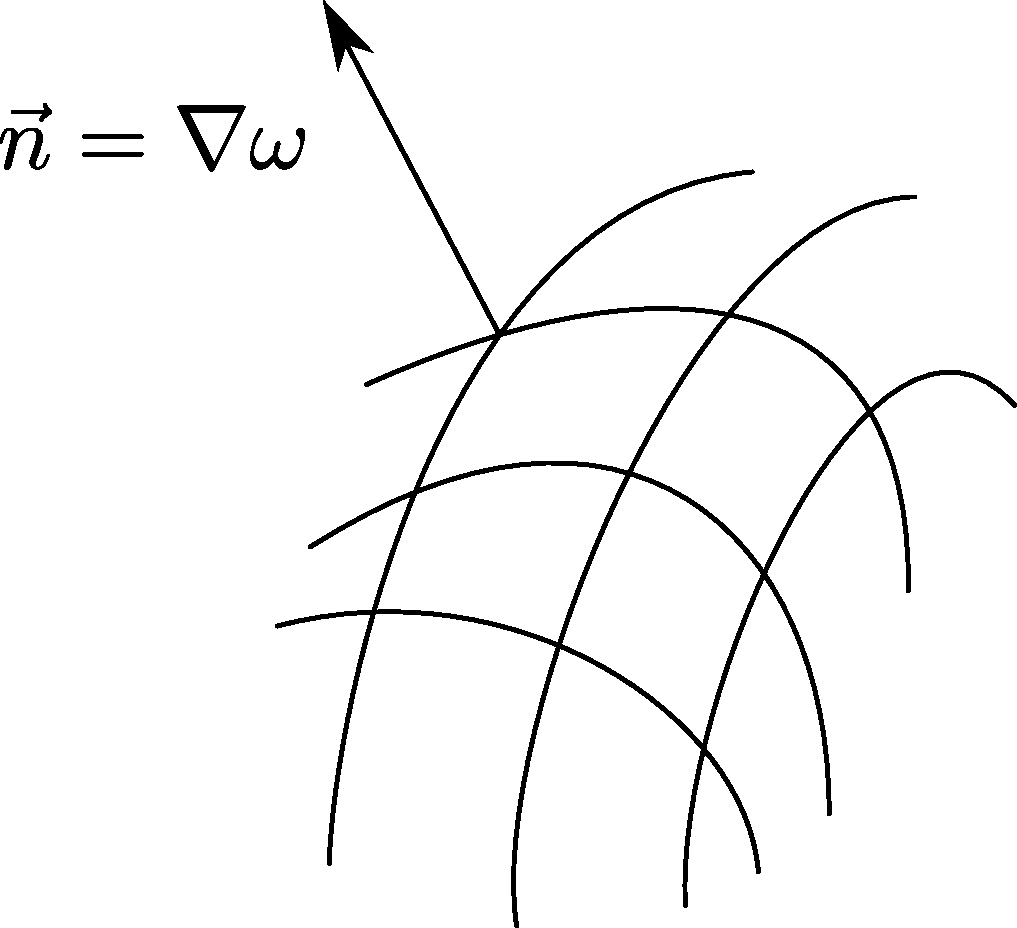
\includegraphics[width=0.34\textwidth]{./pic 2_1.pdf}
\end{center}
\vspace{-0.7em} % Тень на картинке простирается далеко вниз, поэтому кажется, что там есть пустое место. Чтобы его убрать, делаю отрицательное vspace
Дополним $\vec{n}$ до базиса -- получим $\rbrs{\vec{l}_1,\dots,\vec{l}_{n-1},\vec{n}}$. Ортогонализуем -- получим $\rbrs{\vec{e}_1,\dots,\vec{e}_{n-1},\vec{n}}.$ Возьмем такое преобразование:
\[ \vec{y}(\vec{x}) = \begin{cases} y_1 = \brs{\vec{x}-\vec{x}_0} \cdot \vec{e}_1 \\ \vdots \\ y_{n-1} = \brs{\vec{x}-\vec{x}_0} \cdot \vec{e}_{n-1} \\ y_n = \omega(\vec{x}) \end{cases}\]
Проверим, что якобиан не равен 0:

$$
J = \begin{vmatrix} 
\pd{y_1}{x_1} & \cdots & \pd{y_1}{x_n} \\
\cdots &\cdots &\cdots \\
\pd{\omega}{x_1} & \cdots & \pd{\omega}{x_n} \end{vmatrix}
= \begin{vmatrix}
\;(\qquad e_1^T \qquad)\;\\[0.2em]
\cdots\\[0.2em]
\;(\qquad e_n^T \qquad)\;\\[0.6em]
\;(\;\;\: \nabla\omega(x)^T \;\;\:)\;
\end{vmatrix}
\overset{\text{$x = x_0$}}{=\joinrel=}
\begin{vmatrix}
    \;(\qquad e_1^T \qquad)\;\\[0.2em]
    \cdots\\[0.2em]
    \;(\qquad e_n^T \qquad)\;\\[0.6em]
    \;(\qquad n^T \qquad)\;
    \end{vmatrix}
$$

Строки матрицы -- компоненты ОНБ $\Rightarrow J(x_0)\neq 0$.\\
Из соображений непрерывности $J \neq 0$ также в некоторой окрестности точки $x_0$.\\
Значит, это диффеоморфизм класса $C^2$.

В новых переменных: $\displaystyle\sum\limits_{k,l=1}^{n}\hat{a}_{kl}(y)\spd{\hat{u}}{y_k}{y_l} + \hat{F}(y, \hat{u}, \nabla_y \hat{u}) = 0$

Условие характеристичности: \ $\displaystyle 0 = \hat{a}_{nn} = \sum\limits_{i,j=1}^{n} a_{ij}[x(y)]\pd{y_n}{x_i}\pd{y_n}{x_j}$

\begin{definition}[Характеристическая точка]
    Пусть дважды гладкая поверхность $U$ задана уравнением $\omega(x) = 0\quad (\omega \in C^2;$ \ во всех точках $\nabla\omega \neq 0).$\\
    Тогда точка $x_0 \in U$ называется характеристической, если в этой точке $\ \displaystyle\sum\limits_{i,j=1}^{n} a_{ij}\, \omega_{x_i}\, \omega_{x_j} = 0$
\end{definition}

\begin{definition}[Характеристическая поверхность]
    Дважды гладкая поверхность $S$ называется {\bf характеристикой}, если все её точки характеристические.
\end{definition}
\begin{center}
    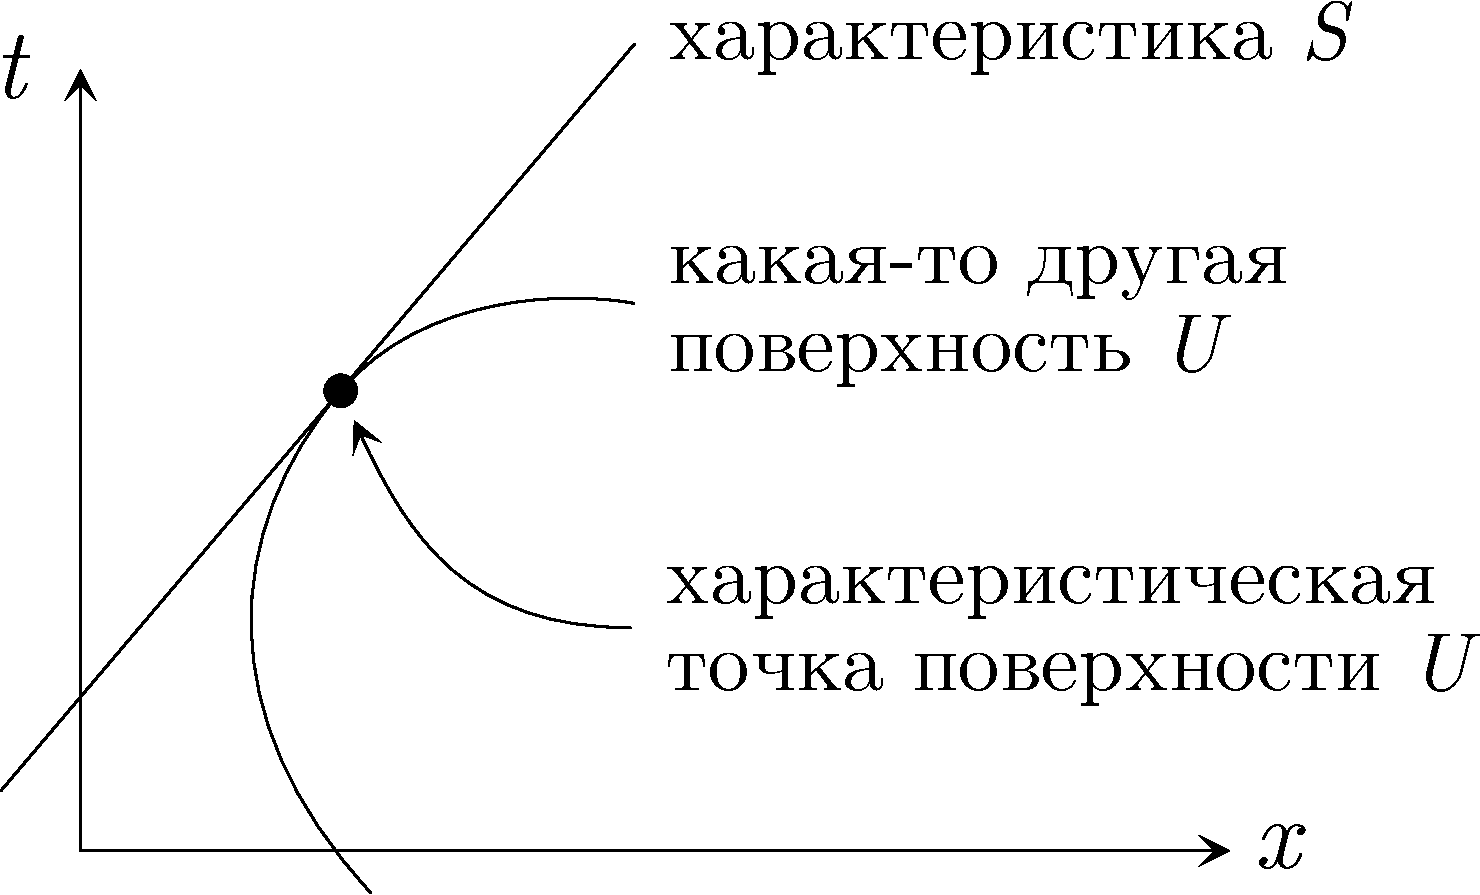
\includegraphics[height=0.22\textwidth]{pic 2_2.pdf}
\end{center}
\begin{example}
$\pdd{u}{x} - \pdd{u}{y} = 0.\quad S$ -- прямая $x=y, \quad \vec{n} = \left(-\dfrac1{\sqrt{2}}, \dfrac1{\sqrt{2}}\right);\quad \pd{u}{\vec{n}} = -\dfrac{u_x}{\sqrt2} + \dfrac{u_y}{\sqrt2} = u_1$

Производная $\dfrac{du_1}{d\vec l} = \left(\vec{l},\; \nabla\,\pd{u}{\vec{n}}\right) = \dfrac1{\sqrt{2}}\pd{}{x}\left[-\dfrac1{\sqrt2}u_x + \dfrac1{\sqrt{2}}u_y\right] + \dfrac1{\sqrt{2}}\pd{}{y}\left[-\dfrac1{\sqrt2}u_x + \dfrac1{\sqrt{2}}u_y\right] = 0.$

Значит, любую функцию на $S$ задать нельзя; прямая $x=y$ -- характеристика.
\end{example}
\vspace{5pt}


\begin{example}
$u_{tt}-a^2\Delta_xu = f(t,x),\ x\in\R^3\ $(волновое уравнение).

Характеристическое уравнение: $\brs{\pd{\omega}{t}}^2 - a^2(\grad \omega)^2 = 0$

Этому уравнению удовлетворяет $\omega(t,x) = \underbrace{a^2t^2 - \vec{x}^2 = 0}_{\text{конус}}$.
\end{example}



\begin{example}
$u_{t}-a^2\Delta_xu = f(t,x)\ $(уравнение теплопроводности).

Характеристическое уравнение: $-a^2[\omega_{x_1}^2 + \dots + \omega_{x_n}^2] = 0\ \Rightarrow \ \omega_{x_i} = 0 \Forall i=\overline{1,n}$

Так как $\nabla \omega \not= 0 $, мы требуем $\omega_t \not=0$. 

Подходит $\omega(t,x) = t-C = 0 \qquad   \Rightarrow \qquad $характеристики --- это гиперплоскости $t=C$
\end{example}



\begin{example}
$\Delta u(x) = f(x)\ \text{(ур-е Пуассона)},\ x\in\R^n;$

Характеристическое уравнение: $\; a^2[\omega_{x_1}^2+\dots+\omega_{x_n}^2] = 0 \ \Rightarrow\ \omega_{x_i} = 0 \Forall i=\overline{1,n}.$

А мы требовали $\nabla \omega \neq 0\ \Rightarrow\ $ у уравнения эллиптического типа нет характеристик.
\end{example}

\bigskip

Функция $u(\vec{x}) = u(x_1,\dots,x_n)$ называется {\bf вещественно-аналитической} в $\vec{x}_0$, если в некоторой $U_{\varepsilon}(\vec{x}_0)$ она представима в виде 
$$u(\vec{x}) = \displaystyle\sum\limits_{|\alpha|>0}u_{\alpha}(\vec{x}-\vec{x}_0)^{\alpha},$$
где $\alpha$ -- мультииндекс, \qquad $u_{\alpha} \in \R, \qquad (\vec{x}-\vec{x}_0)^{\alpha} = (x_1-x_1^0)^{\alpha_1}\cdot\dots\cdot(x-x_n^0)^{\alpha_n}$

\begin{theorem}[Ковалевской]
Пусть в уравнении $\displaystyle\sum\limits_{i,j=1}^{n} a_{ij}(\vec{x})\frac{\partial^2u}{\partial x_i\partial x_j} + F(\vec{x}, u, \nabla u) = 0$:
\begin{itemize}[nolistsep, noitemsep]
\item все $a_{ij}(\vec{x})$ вещественно-аналитические в $\vec{x}_0$ 
\item $F(\vec{x}, u, \nabla u)$ --вещественное-аналитическая в $(\vec{x}_0, u_0(\vec{x}_0), \nabla u(\vec{x}_0))$ соответственно 
\item $\omega(\vec{x})$ вещественно-аналитическая в $\vec{x}_0$
\item $\vec{x}_0$ -- не характеристическая точка $S$
\item $u_0,\ u_1$ -- вещественно-аналитические в $\vec{x}_0$.
\end{itemize}
Тогда: 
\begin{itemize}[nolistsep, noitemsep]
\item $\exists\: U_{\varepsilon}(\vec{x}_0)$ : в ней $\exists$ вещественно-аналитическое решение Задачи Коши (ЗК)
\item оно единственно в классе вещественно-аналитических функций.
\end{itemize}
\end{theorem}

\subsection*{Понятие о корректности}

Рассмотрим абстрактную дифференциальную задачу:

\begin{equation}
\label{eq::2::diff}
\tag{*}
\begin{cases} L(\vec{x}, D)u(\vec{x}) = f(\vec{x}),\ \vec{x} \in \Omega \subseteq \R^n  \\
B_j(\vec{x},D) u(\vec{x}) = g_j(\vec{x}),\ \vec{x}\in \Gamma,\ j\in\overline{1,m},
\end{cases}
\end{equation}
$L$ -- линейный дифференциальный оператор порядка $p$\\
$B_j$ -- конечное семейство линейных дифференциальных операторов в $\Gamma \subset \bar{\Omega}$.

\begin{center}

\includegraphics[width=0.15\textwidth]{pic 2_3.pdf}
\end{center}

\begin{definition}
Пусть $F(\Omega)$ и $U(\Omega)$ -- линейные нормированные пространства функций (ЛНП) на $\Omega$, \; $G_1(\Gamma),\dots G_m(\Gamma)$ -- ЛНП на $\Gamma$.

Тогда если $\ \forall\: f(\vec{x}) \in F(\Omega), \Forall g_j(\vec{x}) \in G_j(\Gamma)$ решение краевой задачи \eqref{eq::2::diff} существует, единственно в $U(\Omega)$ и для него справедлива оценка
\begin{equation}
    \norm{u}_{U(\Omega)} \leq C\norm{f}_{F(\Omega)} + \sum\limits_{j=1}^{m}c_j\norm{g_j}_{G_j(\Gamma)}
\label{eq::2::neq}
\tag{**}
\end{equation}
то {\bf задача корректна по отношению к выбранному набору пространств.}
\end{definition}

\begin{example}[Адамара]
Рассмотрим задачу Коши для уравнения Лапласа:

$\begin{cases} u_{xx}+u_{yy} = 0 \\
u|_{y=0} = u_0(x) = e^{-\sqrt{n}}\cos{nx} \rightrightarrows 0\ \text{вместе со своими производными} \\
u_y|_{y=0} = u_1(x) \equiv 0
\end{cases}$

При $u_0 = 0 \hookrightarrow u\equiv 0$. Если задача корректна, то при увеличении $n$ решения должны $\rightarrow 0$. 

Функции $u_n=e^{-\sqrt{n}}\cos{nx}\ch{ny}$ -- решения.

Но $u_n(0, y^*) = e^{-\sqrt{n}}\ch{ny^*} > \frac1{2}e^{-\sqrt{n}}e^{ny^*} \rightarrow \infty$

Неравенство \eqref{eq::2::neq} не выполнено.
\end{example}
\end{document}
\newpage
\documentclass[../main.tex]{subfiles}
\begin{document}
  
\section{Билет 3. Задача Коши для уравнения колебаний струны. Формула Даламбера. Область зависимости решения от начальных данных. Существование и единственность классического решения. Корректность постановки задачи}
% Затехал: Рязанов Андрей
\textbullet\ Задача $\begin{cases} u_{tt}-a^2u_{xx} = 0\\ \while{u(t,x)}{t=0} = u_0(x)\\ \while{u_t}{t=0} = u_1(x)\end{cases}\quad -l<x<l$

Что понимать под решением задачи?

\begin{definition} \textbf{\emph{Классическое решение}} -- функция класса $C^2$, которая в точках указанной области удовлетворяет уравнению и заданным соотношениям.
\end{definition}

\textbullet\ {\bf Характеристическое уравнение: } $(dx)^2 - a^2(dt)^2 = 0$

$\begin{cases} \xi = x+at \\ \eta = x-at \end{cases} \Leftarrow \begin{cases} x+at = C_1 \\ x-at = C_2 \end{cases}$

В новых координатах $\hat{u}_{\xi\eta}(\xi,\eta) = 0\ \Rightarrow \hat{u} = f(\xi) + g(\eta) $.

Возвращаясь обратно, получим $u(t,x) = f(x+at) + g(x-at)$.
\vspace{0.4em}

\textbullet\ Решим ЗК (поверхности нигде не касаются характеристик -- задача должна быть корректной):
\begin{equation*}
\begin{aligned}
&\while{u}{t=0} = f(x) + g(x) = u_0(x), \quad &-l < x< l&\\
&\while{u_t}{t=0} =  af'(x) - ag'(x) = u_1(x), \quad &-l < x < l& \quad \Rightarrow\ f(x) - g(x) = \frac1{a}\int _{-l}^xu_1(z)dz + C = \frac1{a}V_1(x)
\end{aligned}
\end{equation*}
\begin{center}
$\big\Downarrow$
\end{center}
\begin{equation}
\label{eq::3::dalam}
\tag{*}
\begin{cases} f(x) = \frac1{2}u_0(x) + \frac1{2a}V_1(x) \\ g(x) = \frac1{2}u_0(x) - \frac1{2a}V_1(x) \end{cases} \quad (-l < x< l)
\end{equation}

\[ u(t,x) = \frac1{2}u_0(x+at) + \frac1{2a}V_1(x+at) + \frac1{2}u_0(x-at) - \frac1{2a}V_1(x-at) =\]
\vspace{0.2em}
\[= \boxed{\frac{u_0(x+at) + u_0(x-at)}{2} + \frac1{2a}\int_{x-at}^{x+at}u_1(x)dx} - \text{{\bf формула Даламбера}} \]
\vspace{0.1em}

Решение определяется единственным образом.

Если требуется определить максимальную область, где можно написать решение, то обратимся к формулам \eqref{eq::3::dalam}. Функции $u_0$ и $V$ определены лишь на $(-l;l)\ \Rightarrow\ $искомая область: 

$\begin{cases} -l<x+at<l \\ -l<x-at<l\end{cases}$ -- {\bf характеристический четырехугольник $Q$}.
\bigskip

\begin{wrapfigure}[3]{R}{0.27\textwidth}
\begin{tikzpicture}[scale = 0.5]
  \coordinate (A) at (0, -2);
  \coordinate (B) at (3, 0);
  \coordinate (C) at (0, 2);
  \coordinate (D) at (-3, 0);

  \definecolor{lightGray}{RGB}{216, 216, 216};
  \filldraw[fill = lightGray] (A) -- (B) -- (C) -- (D) -- cycle;


  \draw[->] (-4,0) -- (4,0) node[right] {$x$};
  \draw[->] (0,-3) -- (0,3) node[left] {$y$};

  \coordinate [label = {right: \Large $Q$}] (F) at (0.7, 0);
\end{tikzpicture}
\end{wrapfigure}

Нами доказана теорема:
\begin{theorem}
Пусть $\begin{cases} u_0(x)\in C^2(-l;l) \\ u_1(x) \in C^1(-l;l) \end{cases}$. Тогда ЗК имеет в $Q$\\[0.1em]
единственное решение $u(t,x)\in C^2(Q)$ -- классическое. Оно дается\\[0.1em] 
формулой Даламбера.
\end{theorem}

Корректность задачи для уравнения малых колебаний струны:
\begin{itemize}
\item нами проверены существование и единственность классического решения.
\item покажем непрерывность решения по входным данным $u_0$ и $u_1$.\\Берем две задачи:
\[ 
\begin{cases} 
  \stackrel{\text{\tiny{1}}}{u}_{tt}-a^2\stackrel{\text{\tiny{1}}}{u}_{xx} = 0, \quad (t,x)\in Q\\

  \stackrel{\text{\tiny{1}}}{u}\bigr|_{t=0} = \stackrel{\text{\tiny{1}}}{u}_0(x), \quad \abs{x}<l\\ 
  
  \stackrel{\text{\tiny{1}}}{u}_t\bigr|_{t=0} = \stackrel{\text{\tiny{1}}}{u}_1(x), \quad \abs{x}<l\end{cases} \qquad
\begin{cases} 
  \stackrel{\text{\tiny{2}}}{u}_{tt}-a^2\stackrel{\text{\tiny{2}}}{u}_{xx} = 0, \quad (t,x)\in Q\\

  \stackrel{\text{\tiny{2}}}{u}\bigr|_{t=0} = \stackrel{\text{\tiny{2}}}{u}_0(x), \quad \abs{x}<l\\

  \stackrel{\text{\tiny{2}}}{u}_t\bigr|_{t=0} = \stackrel{\text{\tiny{2}}}{u}_1(x), \quad \abs{x}<l\end{cases}
\]
Пусть $\abs{\stackrel{\text{\tiny{1}}}{u}_0 - \stackrel{\text{\tiny{2}}}{u}_0}<\delta_0,\ \abs{\stackrel{\text{\tiny{1}}}{u}_1 - \stackrel{\text{\tiny{2}}}{u}_1}<\delta_1 \;\Forall x\colon \abs{x}<l.$ \quad Введем 
$\begin{cases}
v_0 = \stackrel{\text{\tiny{1}}}{u}_0 - \stackrel{\text{\tiny{2}}}{u}_0 \\
v_1 = \stackrel{\text{\tiny{1}}}{u}_1 - \stackrel{\text{\tiny{2}}}{u}_1 \\
v = \stackrel{\text{\tiny{1}}}{u} - \stackrel{\text{\tiny{2}}}{u}
\end{cases}$\\
Тогда задача для $v:\ \begin{cases} 
v_{tt}-a^2v_{xx} = 0, \quad (t,x) \in Q\\ 
\while{v}{t=0} = v_0(x),\quad \abs{x}<l,\ \abs{v_0}<\delta_0\\ 
\while{v_t}{t=0} = v_1(x),\quad \abs{x}<l,\ \abs{v_1}<\delta_1
\end{cases}$
\vspace{0.2em}

Согласно формуле Даламбера,
$$\abs{v(t,x)} = \abs{\dfrac{v_0(x+at) + v_0(x-at)}{2} + \dfrac1{2a}\int\limits_{x-at}^{x+at}v_1(y)dy} \leq \delta_0 + \delta_1t \;\; \Forall (t,x) \in Q$$

\begin{itemize}
\item[--] Если $l$ конечно, то $t\le \dfrac{l}{a}$ из вида четырёхугольника $Q$. Устремляя $\delta_0,\, \delta_1 \to 0$, \\
получим $\abs{v}\to 0$.
\item[--] Если $l=\infty$: в любой конечной полосе $t\le T< \infty$ требуемое верно. \\
Так заметаем всю плоскость.


\end{itemize}
\end{itemize}

\end{document}
\newpage
% Сергей Иванычев 
% Затехал Иваныч
\documentclass[../main.tex]{subfiles}
\begin{document}

\section{Билет 4. Смешанная задача для колебаний полубесконечной струны с закрепленным концом. Условия согласования начальных и граничного данных. Существование и единственность классического решения.}

\subsection{Формулировка}

Задача (называется \emph{начально-краевой} или \emph{смешанной})
\begin{equation} \label{4_1}
\begin{cases}
  u_{tt} -a^2u_{xx} = 0 ,\;\;\, t>0,\; x>0 \\
  \begin{aligned}
    \while{u}{t=0}\; &= u_0(x),\quad x\geq 0 \\
    \while{u_t}{t=0} &= u_1(x),\quad x\geq 0  \\
    \while{u}{x=0} &= 0, \;\; \text{по сравнению с задачей Коши это дополнительное граничное условие}
  \end{aligned}
\end{cases}
\end{equation}
\vspace{0pt}  % Почему-то это создаёт дополнительный отступ, которого не хватало

\begin{remark}
    Физический смысл: смотрим, как волна отражается от закрепленного конца  
\end{remark}
Предполагаем, что 
\begin{equation*}
    \begin{cases}
        u_0(x) \in C^2 [0, +\infty) \\
        u_1(x) \in C^1 [0, +\infty) \\
    \end{cases}
\end{equation*}

\subsection{Общее решение}

\begin{align*}
&\ \ u(t,x) = f(x +at) + g(x - at) \\
&\begin{cases}
  \begin{aligned}
    \while{u}{t=0}\; &= f(x) + g(x) = u_0(x), \;\; &x \geq 0\\
    \while{u_t}{t=0} &= af'(x) -ag'(x) = u_1(x), \;\; &x \geq 0  
  \end{aligned}
\end{cases}
\end{align*}
Если ввести обозначение $v_1 = \displaystyle\int_0^x u_1(y)\;dy + C$, то при $x \geq 0$

\begin{wrapfigure}[7]{r}{0.35\textwidth}
    \centering
    
\includegraphics[width=0.35\textwidth]{./pic 4_1.pdf}
\end{wrapfigure}

\begin{align*}
    & f(x) = \frac{1}{2}u_0(x) + \frac{1}{2a}v_1(x) \\
    & g(x) = \frac{1}{2}u_0(x) - \frac{1}{2a}v_1(x) \\
\end{align*}

Граничные условия нужны для определения $u$ в $(x \geq 0)\cap(t \geq 0)$ (в смысле пересечения областей). Их не обязательно ставить на $x=0$, можно на $x + \alpha t = 0, \; -a < \alpha < a$, то есть там, где известна только одна из функций, а не обе.
$$
\while{u}{x=0} = f(at) + g(-at)=0, \;\; t \geq 0
$$
\clearpage % костыль чтобы wrapfigure не думал, что иллюстрация простирается на следующие страницы тоже

\begin{wrapfigure}[7]{r}{0.35\textwidth}
    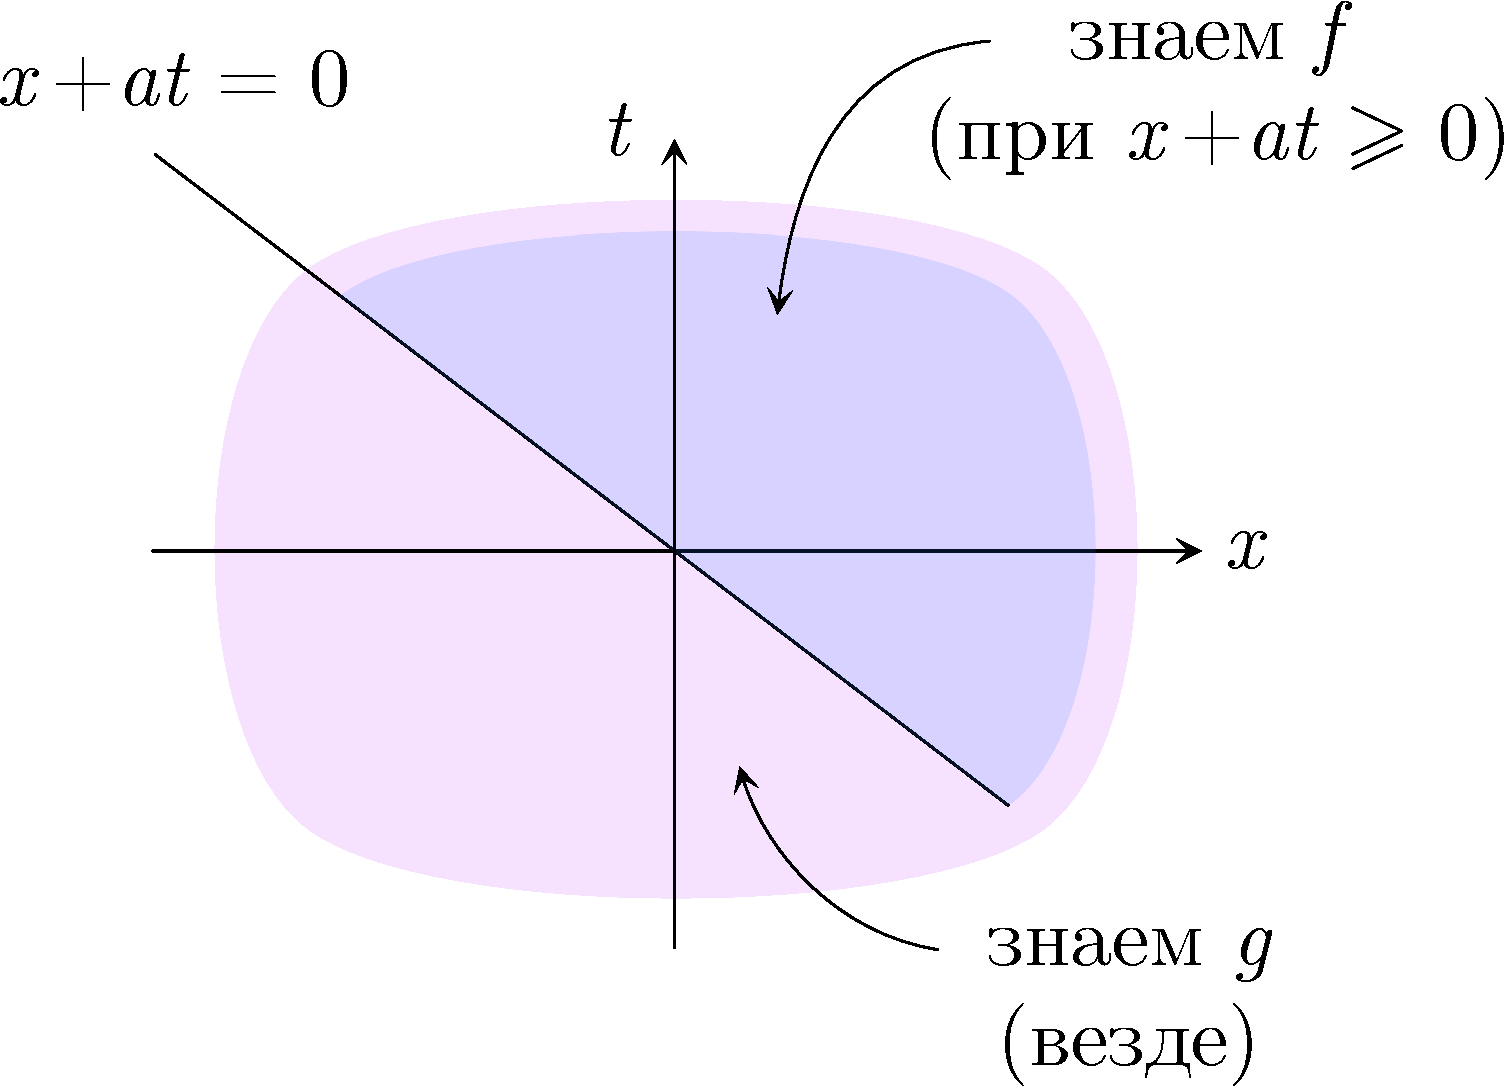
\includegraphics[width=0.35\textwidth]{./pic 4_2.pdf}
\end{wrapfigure}

Введем $\xi = -at, \xi \leq 0$, тогда $g(\xi) = -f(-\xi)$ и суммарно:
\begin{equation*}
    g(\xi) = \begin{cases}
        \frac{1}{2}u_0(\xi)-\frac{1}{2a}v_1(\xi), & \xi \geq 0\\
        -\frac{1}{2}u_0(-\xi)-\frac{1}{2a}v_1(-\xi), & \xi \leq 0\\
    \end{cases}
\end{equation*}

Теперь $g$ известна везде, решение найдено при $x + at > 0$, то есть даже в большей области, чем мы хотели.


\subsection{Сшивка}
Чтобы $g(x) \in C^2(\R)$, решения необходимо <<сшить>>
\begin{align*}
    g(+0) &= g(-0) \\
    g'(+0) &= g'(-0) \\
    g''(+0) &= g''(-0)
\end{align*}
Распишем эти условия:
\begin{align*}
     g(+0) &= g(-0) &\Leftrightarrow&& 
    \frac{1}{2}u_0(0) - \cancel{\frac{1}{2a}v_1(0)} &= -\frac{1}{2}u_0(0) - \cancel{\frac{1}{2a}v_1(0)} &&\Rightarrow& u_0(0) &= 0 \\
     g'(+0) &= g'(-0) &\Leftrightarrow&& \cancel{\frac{1}{2}u'_0(0)} - \frac{1}{2a}u_1(0) &=
    \cancel{\frac{1}{2}u'_0(0)} + \frac{1}{2a}u_1(0) &&\Rightarrow& u_1(0) &= 0 \\
     g''(+0) &= g''(-0) &\Leftrightarrow&& \frac{1}{2} u''_0(0) - \frac{1}{2a} u_1'(0) &= -\frac{1}{2}u_0''(0) - \frac{1}{2a} u_1'(0) &&\Rightarrow& u_0''(0) &= 0
\end{align*}

\begin{definition}[условия согласования]
    Эти условия называются условиями согласования (начальных и граничных условий)
\end{definition}

При их выполнении решение будет классическим. Если $u_0(0) \ne 0$, то даже обобщенного решения не будет.

\subsection{Окончательное решение задачи}

\begin{equation} \label{4_2}
        u(t, x) = \begin{cases}
            \dfrac{u_0(x+at) + u_0(x-at)}{2} + \dfrac{1}{2a}\displaystyle\int_{x-at}^{x+at}u_1(y)\;dy,\quad & \{x\geq -at,\; x\geq at\} \\[1em]

            \dfrac{u_0(at+x) - u_0(at-x)}{2} + \dfrac{1}{2a}\displaystyle\int_{at-x}^{at+x}u_1(y)\;dy,\quad & \{x\geq -at,\; x\leq at\}
        \end{cases}
\end{equation}
\vspace{0pt}

\begin{theorem}
    Пусть в смешанной задаче \ref{4_1} функции $u_0(x)$ и $u_1(x)$ таковы, что 
    \begin{itemize}
        \item Выполнено условие гладкости: $u_0(x)\in C^2[0, +\infty), \; u_1(x) \in C^1[0, +\infty)$
        \item Выполнено условие согласования: $u_0(0) = u_1(0) = u_0''(0) = 0$
    \end{itemize}
    Тогда задача \ref{4_1} имеет единственное классическое решение $u(t,x) \in \C^2(t \geq 0, x\geq 0)$, представленное в \ref{4_2}
\end{theorem}

\begin{proof}
    Используем метод продолжений. Для задачи 
    $$
    \begin{cases}
        u_{tt} -a^2u_{xx} = 0, & t > 0,\; x > 0\\
        \while{u}{t=0} = u_0(x), & x \geq 0\\
        \while{u_t}{t=0} = u_1(x), & x \geq 0\\
        \while{u}{x=0} = 0, & t \geq 0
% у паши тут опечатка
    \end{cases}
    $$  
Введем
$$ \hat u_0(x) = 
\begin{cases}
    u_0(x), & x \geq 0 \\
    -u_0(-x), & x < 0
\end{cases} \qquad \hat u_1(x) = 
\begin{cases}
    u_1(x), & x \geq 0 \\
    -u_1(-x), & x < 0
\end{cases}
$$
Тогда 
$$
\begin{cases}
    \hat u_{tt} -a^2\hat u_{xx} = 0, & t > 0,\; x \in \R^1 \\
    \while{\hat u}{t=0} = \hat u_0(x), & x \in \R^1 \\
    \while{\hat u_t}{t=0} = \hat u_1(x), & x \in \R^1 \\
\end{cases} \; \text{ -- свели к задаче Коши}
$$
\vspace{0pt}

Решение дается формулой Даламбера:
$$
\hat u(t, x) = \frac{\hat u_0(x + at) + \hat u_0(x - at)}{2} +\frac{1}{2a}
\int_{x-at}^{x+at}\hat u_1(y)\;dy
$$

Покажем нечетность по $x$:
\begin{multline*}
\hat u(t, -x) = \frac{\hat u_0(-x + at) + \hat u_0(-x - at)}{2} +\frac{1}{2a}
\int_{-x-at}^{-x+at}\hat u_1(y)\;dy =
\frac{\hat u_0(x - at) + \hat u_0(x + at)}{2} -\\
-\frac{1}{2a}\int_{x-at}^{x+at}\hat u_1(y)\;dy = -\hat u(t, x)
\end{multline*}
\begin{multline*}
\hat u(t, 0) = \underbrace{\frac{\hat u_0(- at) + \hat u_0(at)}{2}}_{=0} + \frac{1}{2a} \int_{-at}^{+at} \hat u_1(y)\;dy = 0\hfill
\end{multline*}
\end{proof}
\end{document}
\newpage
\documentclass[../main.tex]{subfiles}
\begin{document}

\section[Однородное волновое уравнение в \texorpdfstring{$\R^3$}{R\textasciicircum 3}]{Формула Пуассона-Кирхгофа решения задачи Коши для однородного волнового уравнения в $\R^3$. Существование классического решения этой задачи.}
% Затехал: Погодин Роман
\begin{theorem}[Из курса мат. анализа]
Пусть 
$\Omega_x\subset\R^n,\ \Omega_y\subset\R^m$ -- ограниченные области,
$f(x,y)\colon \overline{\Omega}_x \times \overline{\Omega}_y \rightarrow \R,\ 
f \in C \brk*{ \overline{\Omega}_x\times\overline{\Omega}_y }$. 
Тогда 
$J(y) = \displaystyle\int\limits_{\Omega_x} f(x,y)\, dx\ 
\in C \brk*{ \overline{\Omega}_y }$ \\
%
Если к тому же 
$\dfrac{\partial f}{\partial y_k} 
\in C \brk*{ \overline{\Omega}_x\times\overline{\Omega}_y }$, 
то $J(y)$ имеет непрерывную на $\overline{\Omega}_y$ частную производную $\pd{J(y)}{y_k}$, 
которая равна $\displaystyle\int\limits_{\Omega_x} \pd{f}{y_k} (x,y)\, dx.$
\end{theorem}

Обозначим ($\tau$ - вспомогательный параметр)
\[
u_g(t,x,\tau)=\frac{1}{4\pi a^2t}\displaystyle\oiint\limits_{|\xi - x|=at}g(\xi ,\tau )\, dS_{\xi}\, , \qquad a>0,\ t> 0,\ x\in \R^3,\ \tau \geq 0,\ \xi\in\R^3
\]

\begin{lemma}
Пусть $g(\xi, \tau )$ такая, что 
\begin{enumerate}
\item $g \in C\,\{\xi\in\R^3,\ \tau\geq 0 \}$
\item $D_{\xi}^{\alpha}\, g(\xi , \tau )\in C\,\{\xi\in\R^3,\ \tau\geq 0 \} \Forall\alpha\colon |\alpha |\leq p.$
\end{enumerate}

Тогда
\begin{enumerate}

\item $D_{t,x}^{\alpha}\, u_g(t,x,\tau )
      \in C\, \{\mathbf{t\geq 0},\   x\in\R^3,\   \tau \geq 0 \}
      \Forall\alpha\colon |\alpha| \leq p$

\item $\lim\limits_{t\rightarrow +0} u_g(t,x,\tau) = 0$

\item При $p\geq 1$ $\lim\limits_{t\rightarrow +0}\dfrac{\partial u_g}{\partial t}=g(x,\tau)$

\end{enumerate}
\end{lemma}

\begin{proof} Докажем отдельно все три утверждения.
%
\begin{enumerate}
\item Сведем интеграл к интегралу по единичной сфере с центром в нуле с помощью такой замены:
\[
\eta = \frac{\xi - x}{at}
\ \Rightarrow\ 
\xi = x+at\eta,\ |\vec{\eta}|=1.
\]
В таком случае элемент площади $dS_{\xi}=(at)^2dS_{\eta}$. Во введенном выше интеграле получим 
\[
u_g(t,x,\tau) = \frac{(at)^2}{4\pi a^2t}
\oiint\limits_{|\eta|=1}   g(x+at\eta,\,\tau)\,   dS_{\eta} 
= t J_g(t,x,\tau),
\]
где $\displaystyle J_g(t,x,\tau) = \frac{1}{4\pi}
\oiint\limits_{|\eta|=1}   g(x+at\eta,\,\tau)\,   dS_{\eta}$

Теперь интеграл уже по фиксированному множеству. Все выкладки справедливы при $t>0$. Функция
\[
\tilde{g}(t,x,\eta,\tau) = g(x+at\eta,\, \tau)\ 
\in C\, \{t \geq 0,\   x\in\R^3,\   |\eta| = 1,\   \tau \geq 0\}.
\]
Тогда по теореме из начала билета 
$J_g(t,x,\tau) \in C\, \{t\geq 0,\   x\in\R^3,\   \tau \geq 0\}.$

Аналогично будет для производных в силу второй части той же теоремы и наличия соответствующих производных у функции $g$.

\item $\lim\limits_{t\rightarrow +0} U_g(t,x,\tau)
     = \lim\limits_{t\rightarrow +0} t J_g(t,x,\tau)
     = \lim\limits_{t\rightarrow +0} t 
 \cdot \lim\limits_{t\rightarrow +0} J_g(t,x,\tau) = 0$ 
 (последний предел конечен в силу непрерывности).

Можно записать
\[
U_g(t,x,\tau) 
= \begin{cases}
    u_g(t,x, \tau), &t>0\\
    0, &t=0
  \end{cases} \quad 
\in C \brk*{ \overline{\Omega} },
\]
где последнее включение означает непрерывные в области и непрерывно продолжимые на границу функции.

\item При $p\geq 1$ запишем следующее:
\begin{equation*}
\begin{split}
&\lim\limits_{t\rightarrow +0} \pd{}{t} u_g(t,x, \tau) 
=\lim\limits_{t\rightarrow +0} \pd{}{t} \brk[s]*{t J_g(t,x,\tau)}
=\lim\limits_{t\rightarrow +0} J_g(t,x,\tau)
+\cancelto{0}
{\lim\limits_{t\rightarrow +0} t \cdot \pd{}{t} J_g(t,x,\tau)} = \\
%
&= J_g(0, x, \tau) = \frac{1}{4\pi}
\oiint\limits_{|\eta|=1}   g(x+at\eta,\tau)\,   dS_{\eta }
\Biggr|_{t=0}
= g(x,\tau) \frac{1}{4\pi}
\oiint\limits_{|\eta|=1}   dS_{\eta}   =   g(x,\tau).
\end{split}
\end{equation*}
\end{enumerate}
\end{proof}

\imaginarySubsection{Формула Пуассона-Кирхгофа}

Перейдем к решению задачи Коши
\begin{equation}
\begin{cases}
  u_{tt} - a^2\Delta u = 0,   \quad t>0,\   x \in \R^3 \\
  \eval{ u }_{t=0} = 0   \\
  \eval{u_t}_{t=0} = u_1(x)
\end{cases}
\label{eq::5::cauchy}
\end{equation}

\begin{theorem}[Формула Пуассона-Кирхгофа]
Пусть $u_1(x) \in C^2(\R^3)$. Тогда 
\[
u(t,x) = \frac{1}{4\pi a^2t}
\oiint\limits_{|\xi-x|=at}  u_1(\xi)\,  dS_{\xi}   \quad
\in\: C^2\,   \{t\geq 0,\   x \in \R^3 \}
\]
является классическим решением задачи \eqref{eq::5::cauchy}
\end{theorem}

\begin{proof}
В силу леммы имеем 
$\eval{u}_{t=0} = 0;\ \eval{u_t}_{t=0} = u_1$.

Т.к. $u_1 \in C^2(\R^2),\ u \in C^2\,\{t\geq 0, x\in\R^3\}$, то сделаем замену переменной:
\[
u(t,x) = \frac{t}{4\pi}
\oiint\limits_{|\eta|=1}  u_1(x+at\eta)\,  dS_{\eta}.
\]
Осталось только проверить, что $u$ удовлетворяет уравнению
\[
\Delta_x u(x,t) 
= \frac{t}{4\pi}
  \oiint\limits_{|\eta|=1}   \Delta_{\xi} u_1(x+at\eta)\,  dS_{\eta}
= \frac{1}{4\pi a^2t}
  \oiint\limits_{|\xi-x|=at}  \Delta_{\xi} u_1(\xi)\,  dS_{\xi}.
\]
При $t>0$ (использовано $\vec{n} 
     = \dfrac{\xi-x}{|\xi-x|} 
     = \dfrac{\xi-x}{at}   =  \eta$):
\begin{equation*}
\begin{split}
%
&u_t(x,t) = \frac{1}{4\pi}
\oiint\limits_{|\eta|=1}  u_1(x+at\eta)\,  dS_{\eta}
+\frac{ta}{4\pi}
\oiint\limits_{|\eta|=1}
      \sum\limits_{k=1}^3 
      \pd{u_1}{\xi_k} (x+at\eta) \eta_k 
      \cdot dS_{\eta} 
 = \\[0.75em]
%
&=\frac{u(x,t)}{t} + \frac{ta}{4\pi}
\oiint\limits_{|\eta|=1}
       \sum\limits_{k=1}^3 
       \pd{u_1}{\xi_k} (\xi)  n_k(\xi)
       \cdot dS_{\eta}
%
=\frac{u(x,t)}{t} + \frac{1}{4\pi at}
\oiint\limits_{|\xi-x|=at}
       \pd{u_1}{\vec{n}}(\xi) 
       \cdot dS_{\xi}
%
=\frac{u(x,t)}{t} + \frac{1}{4\pi at} I
%
\end{split}
\end{equation*}
Заметим, что
\[
 \iiint\limits_{|\xi-x|<at}  \Delta_{\xi}  u_1(\xi)\,   d\xi 
=\iiint\limits_{|\xi-x|<at}    \div  (\nabla u_1)\,     d\xi 
=\oiint\limits_{|\xi-x|=at}  (\nabla u_1,\, \vec{n})\,  dS_{\xi }
=\oiint\limits_{|\xi-x|=at}     \pd{u_1}{\vec{n}}\,     dS_{\xi }=I
\]
Тогда получим 
$$
u_t = \frac{u}{t} + \frac{1}{4\pi at}
 \iiint\limits_{|\xi-x|<at}  \Delta_{\xi}  u_1(\xi)\,   d\xi \\
%
=\frac{u}{t} + \frac{1}{4\pi at}
\int\limits_0^{at} 
  \left[
    \oiint\limits_{|\xi-x|=\rho}  \Delta_{\xi} u_1(\xi)\,  dS_{\xi}
  \right] d\rho \\
%
=\frac{u}{t} + \frac{1}{4\pi at}
\int\limits_0^{at}  \phi(\rho)\,  d\rho
$$

\begin{equation*}
\begin{split}
&u_{tt}(x,t) = \pd{}{t}
  \left[
    \frac{u}{t} + \frac{I}{4\pi at} 
  \right]
= \frac{u_t}{t} - \frac{u}{t^2}
  - \frac{I}{4\pi at^2} + \frac{I_t}{4\pi at} 
= \frac{u}{t \cdot t} + \frac{I}{4\pi at^2}
  - \frac{u}{t^2} - \frac{I}{4\pi at^2} 
  + \frac{I_t}{4\pi at} = \\
%
&=\frac{I_t}{4\pi at} 
= \frac{1}{4\pi at} \pd{}{t}
  \int\limits_0^{at}  \phi(\rho)\,  d\rho 
= \frac{1}{4\pi at} a \phi(at)
= \frac{1}{4\pi t}
  \oiint\limits_{|\xi-x|=at}  \Delta_{\xi}  u_1(\xi)\,  dS_{\xi}.
\end{split}
\end{equation*}
%
Итак, $u(x, t)$ - классическое решение.
\end{proof}

Рассмотрим
\begin{equation}
\begin{cases}
  u_{tt}-a^2\Delta u=0,\quad t>0,\, x\in \R^3\\
  \eval{u}_{t=0}=u_0(x) \in C^3(\R^3)\\
  \eval{u_t}_{t=0}=0
\end{cases}
\label{eq::5::cauchy2}
\end{equation}

Введем $v(t,x)$:
\[
\begin{cases}
  v_{tt} - a^2 \Delta v=0,  \quad t>0,\ x\in \R^3 \\
  \eval{ v }_{t=0} = 0 \\ 
  \eval{v_t}_{t=0} = u_0(x)
\end{cases}
\]

Эту задачу мы уже решили. Так как $u_0\in C^3(\R^3)$, 
имеем $v\in C^3\, \{t\geq 0,\  x\in\R^3\}$.

\begin{statement}
$u(x,t) \equiv v_t(x, t) \in C^2\, \{t\geq 0,\  x\in\R^3 \}$ 
дает решение задачи \eqref{eq::5::cauchy2}.
\end{statement}

\begin{proof}$\ $
\begin{enumerate}

\item  $u_{tt} - a^2 \Delta u 
= \partial_t (v_{tt} - a^2 \Delta v) 
= \partial_t\: 0 
= 0$

\item $ \eval{u}_{t=0} = \eval{v_t}_{t=0} = u_0(x) $

\item $\eval{u_t}_{t=0} = \eval{v_{tt}}_{t=0} = a^2 \Delta \eval{v}_{t=0} = 0$ 
%
(на гиперплоскости  $t=0  \colon\ 
                 \eval{v}_{t=0} \equiv 0\ \Rightarrow\ 
 \eval*{\pd{v}{x_i}}_{t=0} \equiv 0\ \Rightarrow\ 
\eval*{\pd[2]{v}{x_i}}_{t=0} \equiv 0. $ 
\; При этом $v_t$ может быть ненулевой.)

\end{enumerate}
\end{proof}

Мы доказали следующую теорему:
\begin{theorem}
Функция $u(t,x) = \pd{}{t}
  \left[
    \dfrac{1}{4\pi a^2t}\displaystyle\oiint\limits_{|\xi-x|=at}  u_0(\xi)\,  dS_{\xi } 
  \right],\ 
t \geq 0,\   x\in\R^3$,  где $u_0 \in C^3(\R^3)$, \\[1em]
является классическим решением задачи \eqref{eq::5::cauchy2}. 
\end{theorem}

\end{document}
\newpage
% Сергей Иванычев 
\documentclass[../main.tex]{subfiles}
\begin{document}


\section[Неоднородное волновое уравнение в \texorpdfstring{$\R^3$}{R\textasciicircum 3}]{Формула Кирхгофа решения задачи Коши для неоднородного волнового уравнения в $\R^3$. Метод Дюамеля. Принцип Гюйгенса.}
% Иваныч техал
\subsection*{Формулировка задачи}

\begin{equation} \label{6_1}
    \begin{cases}
        u_{tt} - a^2\Delta u = f(t, x) & t > 0, x \in \R^3 \\
        \eval{u}_{t=0} = 0 & \\
        \eval{u_t}_{t=0} = 0
    \end{cases} \;\;\text{ считаем, что } f(t, x) \in C^{0,2}_{t,x}\, \{t \geq 0,\, x \in \R^3\}
\end{equation}

\Subsection{Метод Дюамеля}

Сведем задачу к задаче Коши для однородного волнового уравнения. Рассмотрим однопараметрическое семейство задач:
\begin{equation} \label{6_2}
\begin{cases}
    w_{tt}(t, x, \tau) - a^2\Delta_x w(t, x, \tau) = 0 & t > \tau;\ x \in \R^3 \\
    \eval{w}_{t=\tau} = 0 & \\
    \eval{w_t}_{t=\tau} = f(\tau, x) &
\end{cases} \;\;\; \tau \geq 0
\end{equation}

Решение задач семейства получаем по формуле Пуассона-Кирхгофа:

\begin{equation*}
    w(t, x, \tau) = \frac{1}{4\pi a^2(t - \tau)}\oiint\limits_{\abs*{\xi - x}=a(t-\tau)}f(\tau, \xi)\,dS_\xi \quad \in \; C^{2,2,0}_{t,x,\tau}\,\{t - \tau \geq 0,\, x \in \R^3\}
\end{equation*}

(Под $C^{2,2,0}_{t,x,\tau}$ подразумевается, что $D^\alpha_{t, x}\: w(t, x, \tau)\in C \Forall \alpha\colon |\alpha| \leq 2$)

\begin{statement}
    $$
    u(t, x) = \int_0^t w(t, x, \tau)d\tau \text{ --- классическое решение исходной задачи.}
    $$
\end{statement}
\begin{proof}\hfill
\begin{itemize}
    \item $u(t,x) \in C^2\, \{x \in \R^3,\; t \geq 0\}$

    \item $\eval{u}_{t=0} = 0$
    
    \item Вычислим $\eval{u_t}_{t=0}$
    
    Интегралы, в которых и пределы, и подынтегральная функция зависят от параметра, дифференциируются по формуле
    $$\pd{}{t} \int_{a(t)}^{b(t)} f(t,x)\,dx = f(t,b(t)) \cdot b' - f(t,a(t)) \cdot a' + \int_{a(t)}^{b(t)} f'_t(t,x)\,dx$$
    В нашем случае $a = 0,\ b = t,\ b' = 1$. Поэтому
    $$\eval{u_t}_{t=0} = 
    \eval*{\brk*{\underbrace{w(t, x, \tau)|_{\tau = t}}_\text{= 0 из нач. усл. в \eqref{6_2}} + \int_0^t \pd{w}{t}d\tau}}_{t=0} = \int_0^0 \pd{w}{t}\, d\tau = 0$$

    \item $\displaystyle \ \Delta_xu = \int_0^t\Delta_x w(t, x, \tau)d\tau$

    \begin{align*}
        u_{tt} &= \pd{}{t}\int_0^t \pd{w}{t}\, d\tau = w_t(t, x, \tau)|_{\tau = t} + \int_0^t w_{tt} (t, x, \tau)\, d\tau
        = f(\tau, x)|_{\tau = t} + a^2 \int_0^t \Delta_x w(t, x, \tau) \, d\tau \\[0.5em]
        &= f(t, x) + a^2\Delta_x u
    \end{align*}
\end{itemize}

Значит, рассматриваемая функция удовлетворяет уравнению.
\end{proof}
Мы доказали следующую теорему:
\begin{theorem}
    Пусть в  задаче \eqref{6_1} функция $f(t,x)$ такова, что $D^\alpha_x\, f \in C\,\{t \geq 0,\; x \in \R^3\}$\\ 
    Тогда функция 
    \begin{equation} \label{6_3}
        u(t, x) = \int\limits_0^t{ \frac{1}{4\pi a^2(t - \tau)}
        \brk[s]*{\oiint\limits_{\;\abs*{\xi - x} = a(t - \tau)}
        f(\tau, \xi)\, dS_\xi} d\tau}
    \end{equation}
    является классическим решением, причем 
    $$
    D^\alpha_{t, x}\, u \in C\,\{t \geq 0, x \in \R^3\}
    $$
\end{theorem}
Суть метода Дюамеля: $f(t, x)$ --- это начальные данные в каждый момент времени.

\Subsection{Запаздывающий потенциал}
Преобразуем формулу \eqref{6_3}: 
\begin{align*}
    &\int\limits_0^t \frac{d\tau}{4\pi a^2(t - \tau)}
    \oiint\limits_{\abs*{\xi - x} = a(t - \tau)} f(\tau, \xi)\, dS_\xi = 
    \begin{bmatrix} 
        \rho = a(t - \tau) \\
        \tau = t -\rho/a \\
        d\tau = -d\rho/a 
    \end{bmatrix} = 
    -\int\limits_{at}^0 \frac{1}{4\pi a \rho} \frac{d\rho}{a} 
    \oiint\limits_{\abs*{\xi - x} = \rho} f \brk*{t - \frac{\rho}{a},\; \xi} dS_\xi = \\[1em]
    &= \frac{1}{4\pi a^2} \int\limits_0^{at} d\rho \oiint\limits_{\abs*{\xi - x} = \rho} \frac{f(t - \frac{\abs*{\xi - x}}{a},\; \xi)}{\abs*{\xi - x}}\, dS_\xi
    = \boxed{\frac{1}{4\pi a^2} \iiint\limits_{\abs*{\xi - x} < at}\frac{f(t - \frac{\abs*{\xi - x}}{a}, \xi)}{\abs*{\xi - x}}\;d\xi}
\end{align*}

Выражение в рамке называется \emph{запаздывающим потенциалом}.

\Subsection[Общая формула Кирхгофа]{Общая задача Коши:}
\vspace{-0.5em}
$$
\begin{cases}
    u_{tt} - a^2\Delta_x u = f(t, x) \\
    \eval{u}_{t=0} = u_0(x) \\
    \eval{u_t}_{t=0} = u_1(x)
\end{cases}
$$
\vspace{0em} % По какой-то причине это добавляет ненулевое vspace именно той величины, которое нужно

\begin{theorem}[формула Кирхгофа]
    Пусть в общей задаче Коши
    $$
    u_0 \in C^3(\R^3) \qquad 
    u_1 \in C^2(\R^3) \qquad 
    f \in C^{0,2}_{t,x}\,\{t \geq 0,\; x \in \R^3\} $$
    Тогда выражение
    \begin{equation*} \label{6_4}
        u(t, x) = \pd{}{t} \frac{1}{4\pi a^2t}\oiint\limits_{\abs*{\xi - x}=at}u_0(\xi)\, dS_\xi
        + \frac{1}{4\pi a^2t} \oiint\limits_{\abs*{\xi - x}=at}u_1(\xi)\, dS_\xi 
        + \frac{1}{4\pi a^2} \iiint\limits_{\abs*{\xi - x} < at} \frac{f(t - \frac{\abs*{\xi - x}}{a}, \xi)}{\abs*{\xi - x}}\, d\xi
    \end{equation*}

    является классическим решением общей задачи Коши; \; $u(t,x) \in C^2\,\{t \geq 0,\ x \in \R^3\}$
\end{theorem}

\Subsection{Принцип Гюйгенса}

\begin{statement}[Принцип Гюйгенса]
    Возмущение, локализованное в пространстве (трёхмерном), приводит к действию, локализованному во времени.
\end{statement}

% Требуется отсутствие источников: $f \equiv 0$ -- и ограниченность носителей функций $u_0$ и $u_1$:
Требуется, чтобы 
источники отсутствовали, т.е.
$f \equiv 0$, а носители функций $u_0$ и $u_1$ были ограничены, откуда
$$\supp u_0 \ \cup\ \supp u_1 = M \text{ --- компакт}$$

Фиксируется произвольная точка $x_0 \in \R^3$.

По \hyperref[6_4]{формуле Кирхгофа} функция $u(t, x_0)$ может быть ненулевой только внутри отрезка времени
$$
\text{от \ } t_\text{start} = \frac{1}{a} \cdot \inf_{y\in M}|y-x_0|
\qquad \text{ \ до \ } t_\text{end} = \frac{1}{a} \cdot \sup_{y \in M}|y-x_0|
$$
(иначе под интегралами тождественный нуль).

У такого конечного возмущения есть передний и задний фронт:
\vspace{0.7em}

\centering
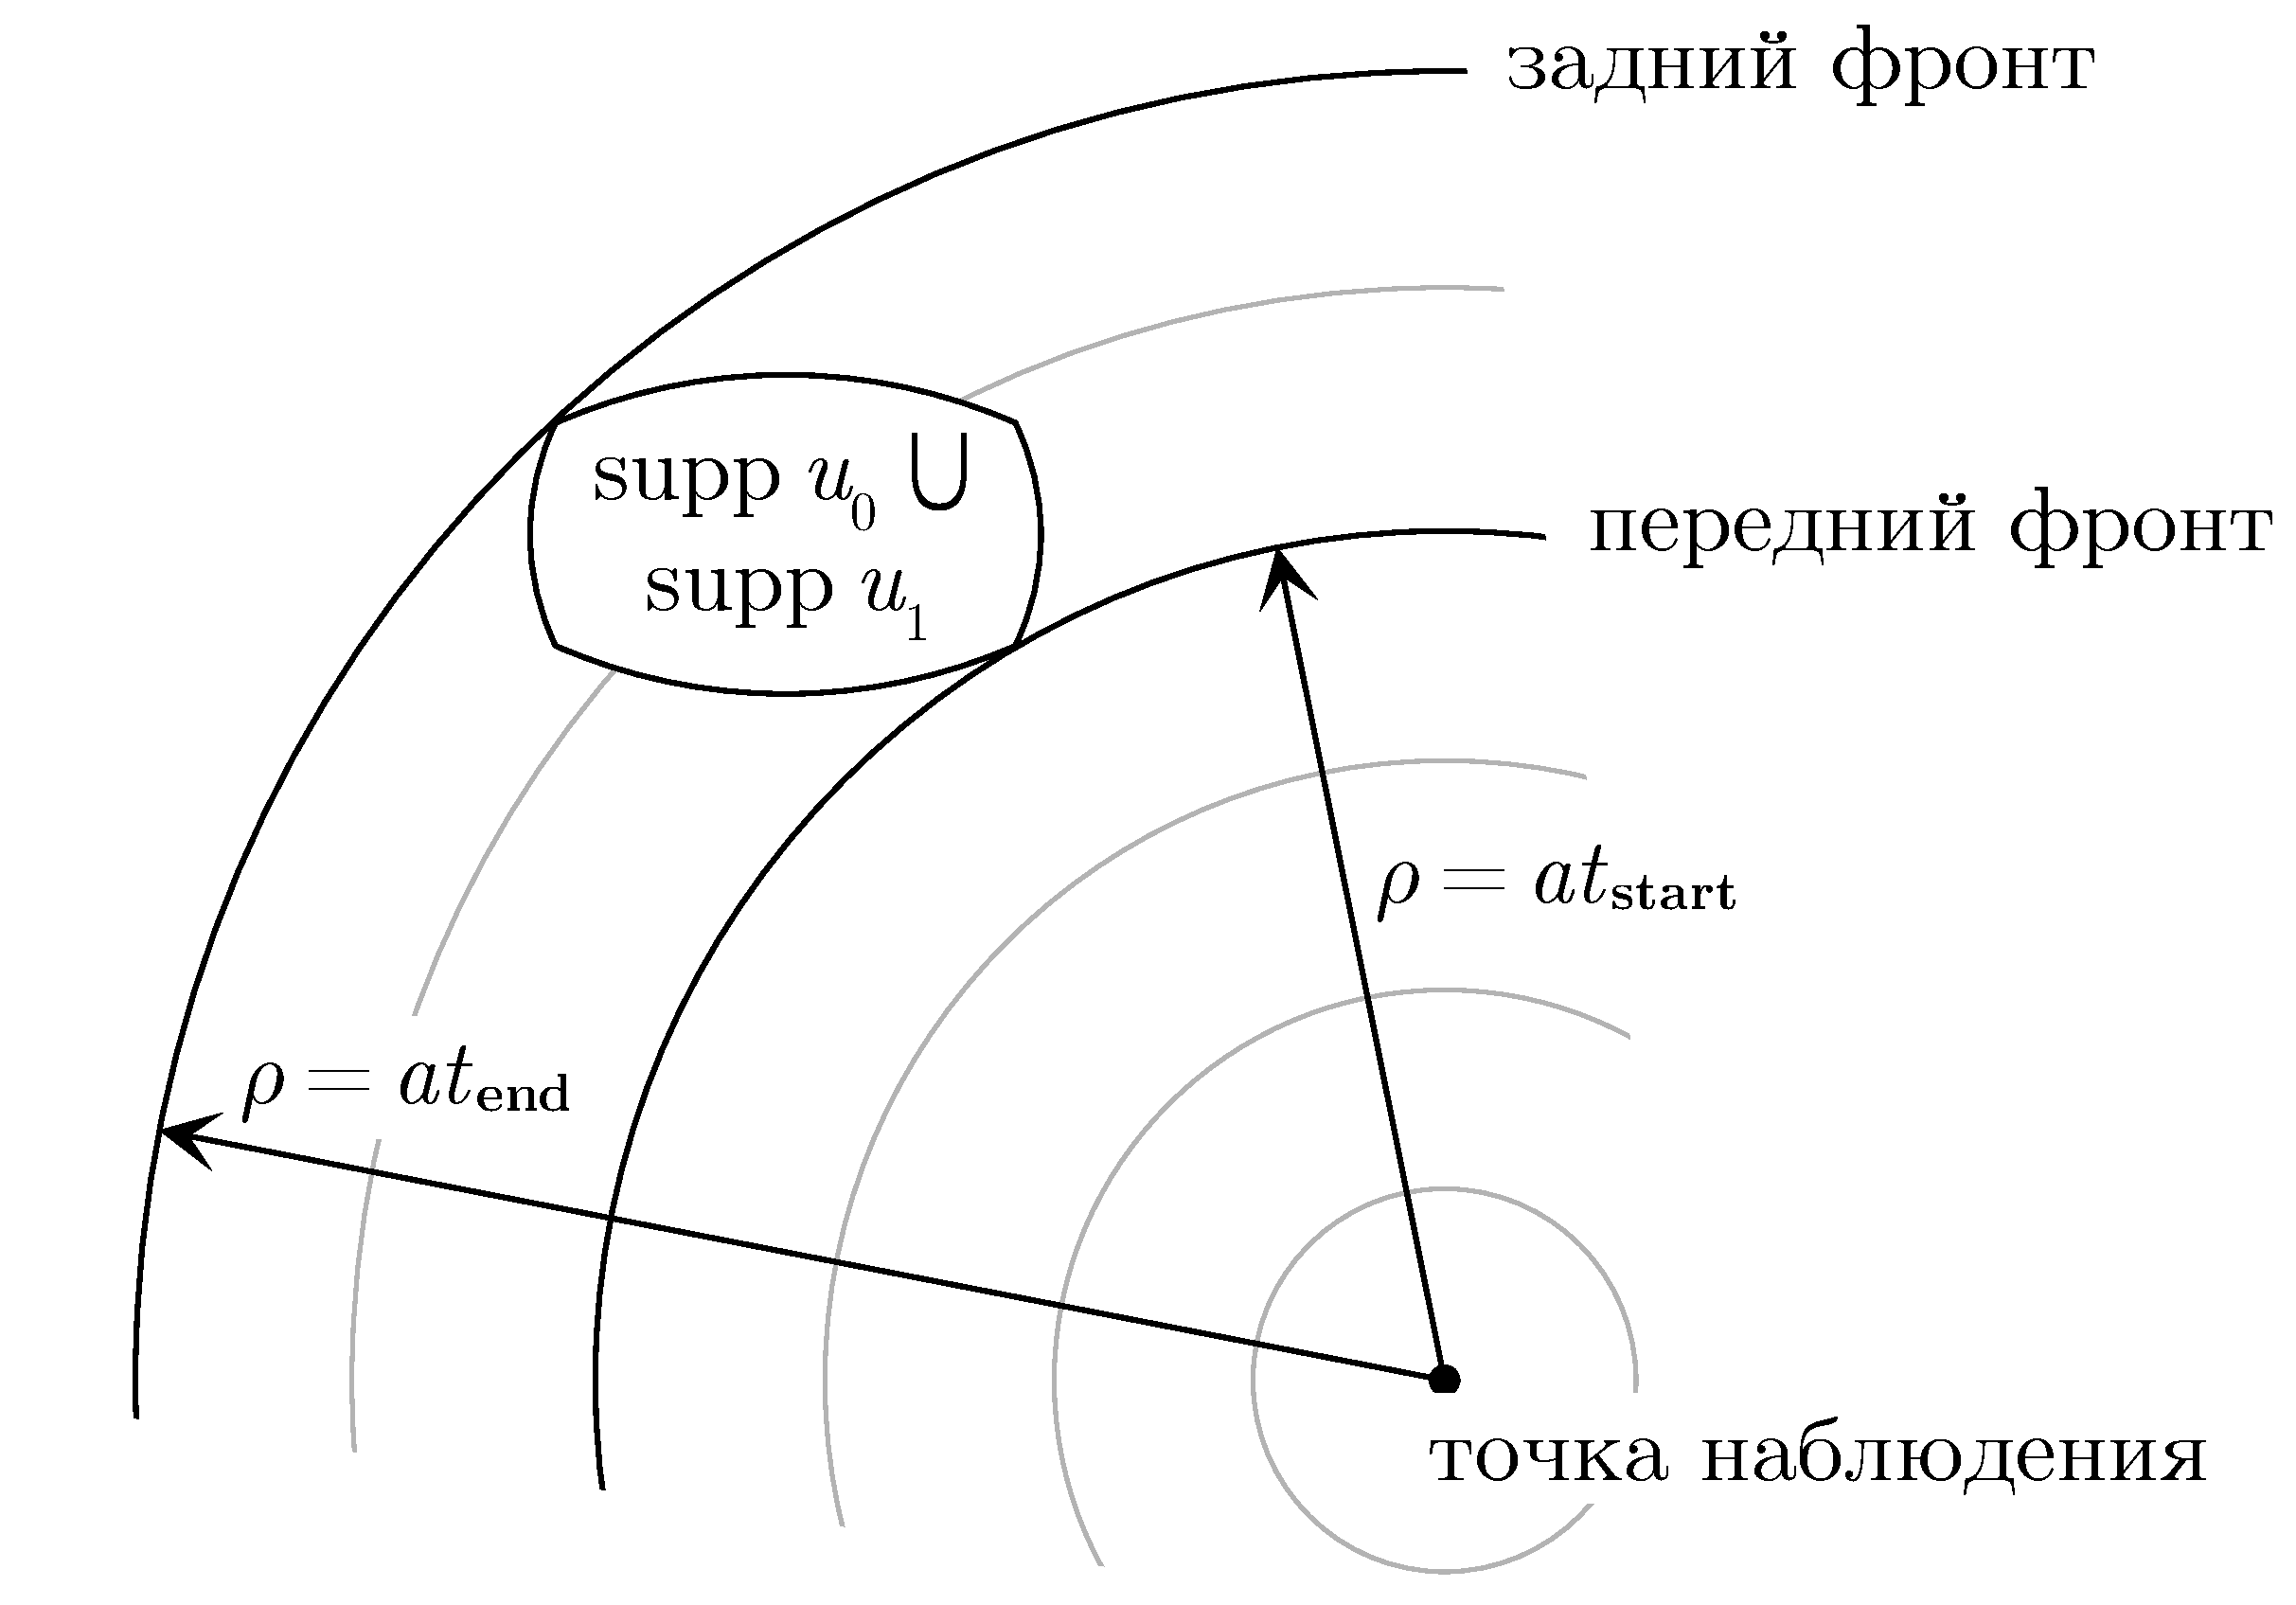
\includegraphics[width=0.45\textwidth]{./pic 6.pdf}

Значение $u(t,x_0)$ \ $\sim$ \ интеграл по сфере радиусом $|x_0 -\xi| = \rho = at$

\end{document}

\newpage
\documentclass[../main.tex]{subfiles}
\begin{document}

\section[Однородное волновое уравнение в \texorpdfstring{$\R^3$}{R\textasciicircum 3}]{Формула Пуассона-Кирхгофа решения задачи Коши для однородного волнового уравнения в $\R^3$. Существование классического решения этой задачи.}
% Затехал: Погодин Роман
\begin{theorem}[Из курса мат. анализа]
Пусть 
$\Omega_x\subset\R^n,\ \Omega_y\subset\R^m$ -- ограниченные области,
$f(x,y)\colon \overline{\Omega}_x \times \overline{\Omega}_y \rightarrow \R,\ 
f \in C \brk*{ \overline{\Omega}_x\times\overline{\Omega}_y }$. 
Тогда 
$J(y) = \displaystyle\int\limits_{\Omega_x} f(x,y)\, dx\ 
\in C \brk*{ \overline{\Omega}_y }$. \\
%
Если к тому же 
$\dfrac{\partial f}{\partial y_k} 
\in C \brk*{ \overline{\Omega}_x\times\overline{\Omega}_y }$, 
то $J(y)$ имеет непрерывную на $\overline{\Omega}_y$ частную производную $\pd{J(y)}{y_k}$, 
которая равна $\displaystyle\int\limits_{\Omega_x} \pd{f}{y_k} (x,y)\, dx.$
\end{theorem}

\begin{lemma}
Пусть $g(\tau, \xi) \in C^{0,\, p}_{\tau,\, \xi} \,\brk[c]!{\tau \geq 0,\ \xi \in \R^3}$. Введём $u_g(t, x, \tau)\colon$
\[
u_g(t,x,\tau) \coloneqq \frac{1}{4\pi a^2t}\oiint\limits_{|\xi - x|=at}g(\tau, \xi)\, dS_{\xi}\, , \qquad a>0,\ t> 0,\ x\in \R^3,\ \tau \geq 0,\ \xi\in\R^3
\]
Тогда
\begin{enumerate}

\item $u_g \in C^{p,\, p,\, 0}_{t,\, x,\, \tau}\, \brk[c]!{\mathbf{t \geq 0},\ x \in \R^3, \tau \geq 0}$

\item $\lim\limits_{t\rightarrow +0} u_g(t,x,\tau) = 0$

\item При $p\geq 1$ $\lim\limits_{t\rightarrow +0}\dfrac{\partial u_g}{\partial t}=g(\tau, x)$

\end{enumerate}
\end{lemma}

(Под $C^{p,\, p,\, 0}_{t,\, x,\, \tau}$ подразумевается, что $D_{t,x}^{\alpha}\, u_g(t,x,\tau) \in C \Forall\alpha\colon |\alpha| \leq p$)
\footnote{Если расписать мультииндексы: \ $\partial^{\alpha_0}_t    \, 
\partial^{\alpha_1}_{x_1} \, 
\partial^{\alpha_2}_{x_2} \,
\partial^{\alpha_3}_{x_3} \; 
u_g(t, x, \tau) 
\in C \;\Forall \alpha_i \colon \sum\limits_{i=0}^{3} \alpha_i \leq p$}

\begin{proof} Докажем отдельно все три утверждения.
%
\begin{enumerate}
\item Сведем интеграл к интегралу по единичной сфере с центром в нуле с помощью такой замены:
\[
\eta = \frac{\xi - x}{at}
\ \Rightarrow\ 
\xi = x+at\eta,\ |\vec{\eta}|=1.
\]
В таком случае элемент площади $dS_{\xi}=(at)^2dS_{\eta}$. Во введенном выше интеграле получим 
\[
u_g(t,x,\tau) = \frac{(at)^2}{4\pi a^2t}
\oiint\limits_{|\eta|=1}   g(\tau,\, x+at\eta)\,   dS_{\eta} 
= t J_g(t,x,\tau),
\]
где $\displaystyle J_g(t,x,\tau) = \frac{1}{4\pi}
\oiint\limits_{|\eta|=1}   g(\tau,\, x+at\eta)\,   dS_{\eta}$

Теперь интеграл уже по фиксированному множеству. Все выкладки справедливы при $t>0$. Функция
\[
\tilde{g}(t,x,\eta,\tau) = g(\tau,\, x+at\eta)\ 
\in C\, \{t \geq 0,\   x\in\R^3,\   |\eta| = 1,\   \tau \geq 0\}.
\]
Тогда по теореме из начала билета 
$J_g(t,x,\tau) \in C\, \{t\geq 0,\   x\in\R^3,\   \tau \geq 0\}.$

Аналогично будет для производных в силу второй части той же теоремы и наличия соответствующих производных у функции $g$.

\item $\lim\limits_{t\rightarrow +0} U_g(t,x,\tau)
     = \lim\limits_{t\rightarrow +0} t J_g(t,x,\tau)
     = \lim\limits_{t\rightarrow +0} t 
 \cdot \lim\limits_{t\rightarrow +0} J_g(t,x,\tau) = 0$ 
 (последний предел конечен в силу непрерывности).

Можно записать
\[
U_g(t,x,\tau) 
= \begin{cases}
    u_g(t,x, \tau), &t>0,\\
    0, &t=0,
  \end{cases} \quad 
\in C \brk*{ \overline{\Omega} },
\]
где последнее включение означает непрерывные в области и непрерывно продолжимые на границу функции.

\item При $p\geq 1$ запишем следующее:
\begin{equation*}
\begin{split}
&\lim\limits_{t\rightarrow +0} \pd{}{t} u_g(t,x, \tau) 
=\lim\limits_{t\rightarrow +0} \pd{}{t} \brk[s]*{t J_g(t,x,\tau)}
=\lim\limits_{t\rightarrow +0} J_g(t,x,\tau)
+\cancelto{0}
{\lim\limits_{t\rightarrow +0} t \cdot \pd{}{t} J_g(t,x,\tau)} = \\
%
&= J_g(0, x, \tau) = \frac{1}{4\pi}
\oiint\limits_{|\eta|=1}   g(\tau, x+at\eta)\,   dS_{\eta }
\Biggr|_{t=0}
= g(\tau, x) \frac{1}{4\pi}
\oiint\limits_{|\eta|=1}   dS_{\eta}   =   g(\tau, x).
\end{split}
\end{equation*}
\end{enumerate}
\end{proof}

\imaginarySubsection{Формула Пуассона-Кирхгофа}

Перейдем к решению задачи Коши
\begin{equation}
\begin{cases}
  u_{tt} - a^2\Delta u = 0,   \quad t>0,\   x \in \R^3, \\
  \eval{ u }_{t=0} = 0,   \\
  \eval{u_t}_{t=0} = u_1(x).
\end{cases}
\label{eq::7::cauchy}
\end{equation}

\begin{theorem}[Формула Пуассона-Кирхгофа]
Пусть $u_1(x) \in C^2(\R^3)$. Тогда 
\[
u(t,x) = \frac{1}{4\pi a^2t}
\oiint\limits_{|\xi-x|=at}  u_1(\xi)\,  dS_{\xi}   \quad
\in\: C^2\,   \{t\geq 0,\   x \in \R^3 \}
\]
является классическим решением задачи \eqref{eq::7::cauchy}.
\end{theorem}

\begin{proof}
В силу леммы имеем 
$\eval{u}_{t=0} = 0;\ \eval{u_t}_{t=0} = u_1$.

Т.к. $u_1 \in C^2(\R^3),\ u \in C^2\,\{t\geq 0, x\in\R^3\}$, то сделаем замену переменной:
\[
u(t,x) = \frac{t}{4\pi}
\oiint\limits_{|\eta|=1}  u_1(x+at\eta)\,  dS_{\eta}.
\]
Осталось только проверить, что $u$ удовлетворяет уравнению
\[
\Delta_x u(x,t) 
= \frac{t}{4\pi}
  \oiint\limits_{|\eta|=1}   \Delta_{\xi} u_1(x+at\eta)\,  dS_{\eta}
= \frac{1}{4\pi a^2t}
  \oiint\limits_{|\xi-x|=at}  \Delta_{\xi} u_1(\xi)\,  dS_{\xi}.
\]
При $t>0$ (использовано $\vec{n} 
     = \dfrac{\xi-x}{|\xi-x|} 
     = \dfrac{\xi-x}{at}   =  \eta$):
\begin{equation*}
\begin{split}
%
&u_t(x,t) = \frac{1}{4\pi}
\oiint\limits_{|\eta|=1}  u_1(x+at\eta)\,  dS_{\eta}
+\frac{ta}{4\pi}
\oiint\limits_{|\eta|=1}
      \sum\limits_{k=1}^3 
      \pd{u_1}{\xi_k} (x+at\eta) \eta_k 
      \cdot dS_{\eta} 
 = \\[0.75em]
%
&=\frac{u(x,t)}{t} + \frac{ta}{4\pi}
\oiint\limits_{|\eta|=1}
       \sum\limits_{k=1}^3 
       \pd{u_1}{\xi_k} (\xi)  n_k(\xi)
       \cdot dS_{\eta}
%
=\frac{u(x,t)}{t} + \frac{1}{4\pi at}
\oiint\limits_{|\xi-x|=at}
       \pd{u_1}{\vec{n}}(\xi) 
       \cdot dS_{\xi}
%
=\frac{u(x,t)}{t} + \frac{1}{4\pi at} I
%
\end{split}
\end{equation*}
Заметим, что
\[
 \iiint\limits_{|\xi-x|<at}  \Delta_{\xi}  u_1(\xi)\,   d\xi 
=\iiint\limits_{|\xi-x|<at}    \div  (\nabla u_1)\,     d\xi 
=\oiint\limits_{|\xi-x|=at}  (\nabla u_1,\, \vec{n})\,  dS_{\xi }
=\oiint\limits_{|\xi-x|=at}     \pd{u_1}{\vec{n}}\,     dS_{\xi }=I
\]
Тогда получим 
$$
u_t = \frac{u}{t} + \frac{1}{4\pi at}
 \iiint\limits_{|\xi-x|<at}  \Delta_{\xi}  u_1(\xi)\,   d\xi \\
%
=\frac{u}{t} + \frac{1}{4\pi at}
\int\limits_0^{at} 
  \left[
    \oiint\limits_{|\xi-x|=\rho}  \Delta_{\xi} u_1(\xi)\,  dS_{\xi}
  \right] d\rho \\
%
=\frac{u}{t} + \frac{1}{4\pi at}
\int\limits_0^{at}  \phi(\rho)\,  d\rho
$$

\begin{equation*}
\begin{split}
&u_{tt}(x,t) = \pd{}{t}
  \left[
    \frac{u}{t} + \frac{I}{4\pi at} 
  \right]
= \frac{u_t}{t} - \frac{u}{t^2}
  - \frac{I}{4\pi at^2} + \frac{I_t}{4\pi at} 
= \frac{1}{t} \cdot \left( \frac{u}{t} + \frac{I}{4\pi at} \right)
  - \frac{u}{t^2} - \frac{I}{4\pi at^2} 
  + \frac{I_t}{4\pi at} = \\
%
&=\frac{I_t}{4\pi at} 
= \frac{1}{4\pi at} \pd{}{t}
  \int\limits_0^{at}  \phi(\rho)\,  d\rho 
= \frac{1}{4\pi at} a \phi(at)
= \frac{1}{4\pi t}
  \oiint\limits_{|\xi-x|=at}  \Delta_{\xi}  u_1(\xi)\,  dS_{\xi}.
\end{split}
\end{equation*}
%
Итак, $u(x, t)$ -- классическое решение.
\end{proof}

Рассмотрим
\begin{equation}
\begin{cases}
  u_{tt}-a^2\Delta u=0,\quad t>0,\, x\in \R^3\\
  \eval{u}_{t=0}=u_0(x) \in C^3(\R^3),\\
  \eval{u_t}_{t=0}=0.
\end{cases}
\label{eq::7::cauchy2}
\end{equation}

Введем $v(t,x)$:
\[
\begin{cases}
  v_{tt} - a^2 \Delta v=0,  \quad t>0,\ x\in \R^3 \\
  \eval{ v }_{t=0} = 0, \\ 
  \eval{v_t}_{t=0} = u_0(x).
\end{cases}
\]

Эту задачу мы уже решили. Так как $u_0\in C^3(\R^3)$, 
имеем $v\in C^3\, \{t\geq 0,\  x\in\R^3\}$.

\begin{statement}
$u(x,t) \equiv v_t(x, t) \in C^2\, \{t\geq 0,\  x\in\R^3 \}$ 
дает решение задачи \eqref{eq::7::cauchy2}.
\end{statement}

\begin{proof}$\ $
\begin{enumerate}

\item  $u_{tt} - a^2 \Delta u 
= \partial_t (v_{tt} - a^2 \Delta v) 
= \partial_t\: 0 
= 0$

\item $ \eval{u}_{t=0} = \eval{v_t}_{t=0} = u_0(x) $

\item $\eval{u_t}_{t=0} = \eval{v_{tt}}_{t=0} = a^2 \Delta \eval{v}_{t=0} = 0$ 
%
(на гиперплоскости  $t=0  \colon\ 
                 \eval{v}_{t=0} \equiv 0\ \Rightarrow\ 
 \eval*{\pd{v}{x_i}}_{t=0} \equiv 0\ \Rightarrow\ 
\eval*{\pd[2]{v}{x_i}}_{t=0} \equiv 0. $ 
\; При этом $v_t$ может быть ненулевой.)

\end{enumerate}
\end{proof}

Мы доказали следующую теорему:
\begin{theorem}
Функция $u(t,x) = \pd{}{t}
  \left[
    \dfrac{1}{4\pi a^2t}\displaystyle\oiint\limits_{|\xi-x|=at}  u_0(\xi)\,  dS_{\xi } 
  \right],\ 
t \geq 0,\   x\in\R^3$,  где $u_0 \in C^3(\R^3)$, \\[1em]
является классическим решением задачи \eqref{eq::7::cauchy2}. 
\end{theorem}


\Subsection{Принцип Гюйгенса}

\begin{statement}[Принцип Гюйгенса]
    Возмущение, локализованное в пространстве (трёхмерном), приводит к действию, локализованному во времени.
\end{statement}

% Требуется отсутствие источников: $f \equiv 0$ -- и ограниченность носителей функций $u_0$ и $u_1$:
Требуется, чтобы 
источники отсутствовали, т.е.
$f \equiv 0$, а носители функций $u_0$ и $u_1$ были ограничены, откуда
$$\supp u_0 \ \cup\ \supp u_1 = M \text{ -- компакт}$$

Фиксируется произвольная точка $x_0 \in \R^3$.

По формуле Кирхгофа функция $u(t, x_0)$ может быть ненулевой только внутри отрезка времени
$$
\text{от \ } t_\text{start} = \frac{1}{a} \cdot \inf_{y\in M}|y-x_0|
\qquad \text{ \ до \ } t_\text{end} = \frac{1}{a} \cdot \sup_{y \in M}|y-x_0|
$$
(иначе под интегралами тождественный нуль).

У такого конечного возмущения есть передний и задний фронт:
\vspace{0.7em}

\centering
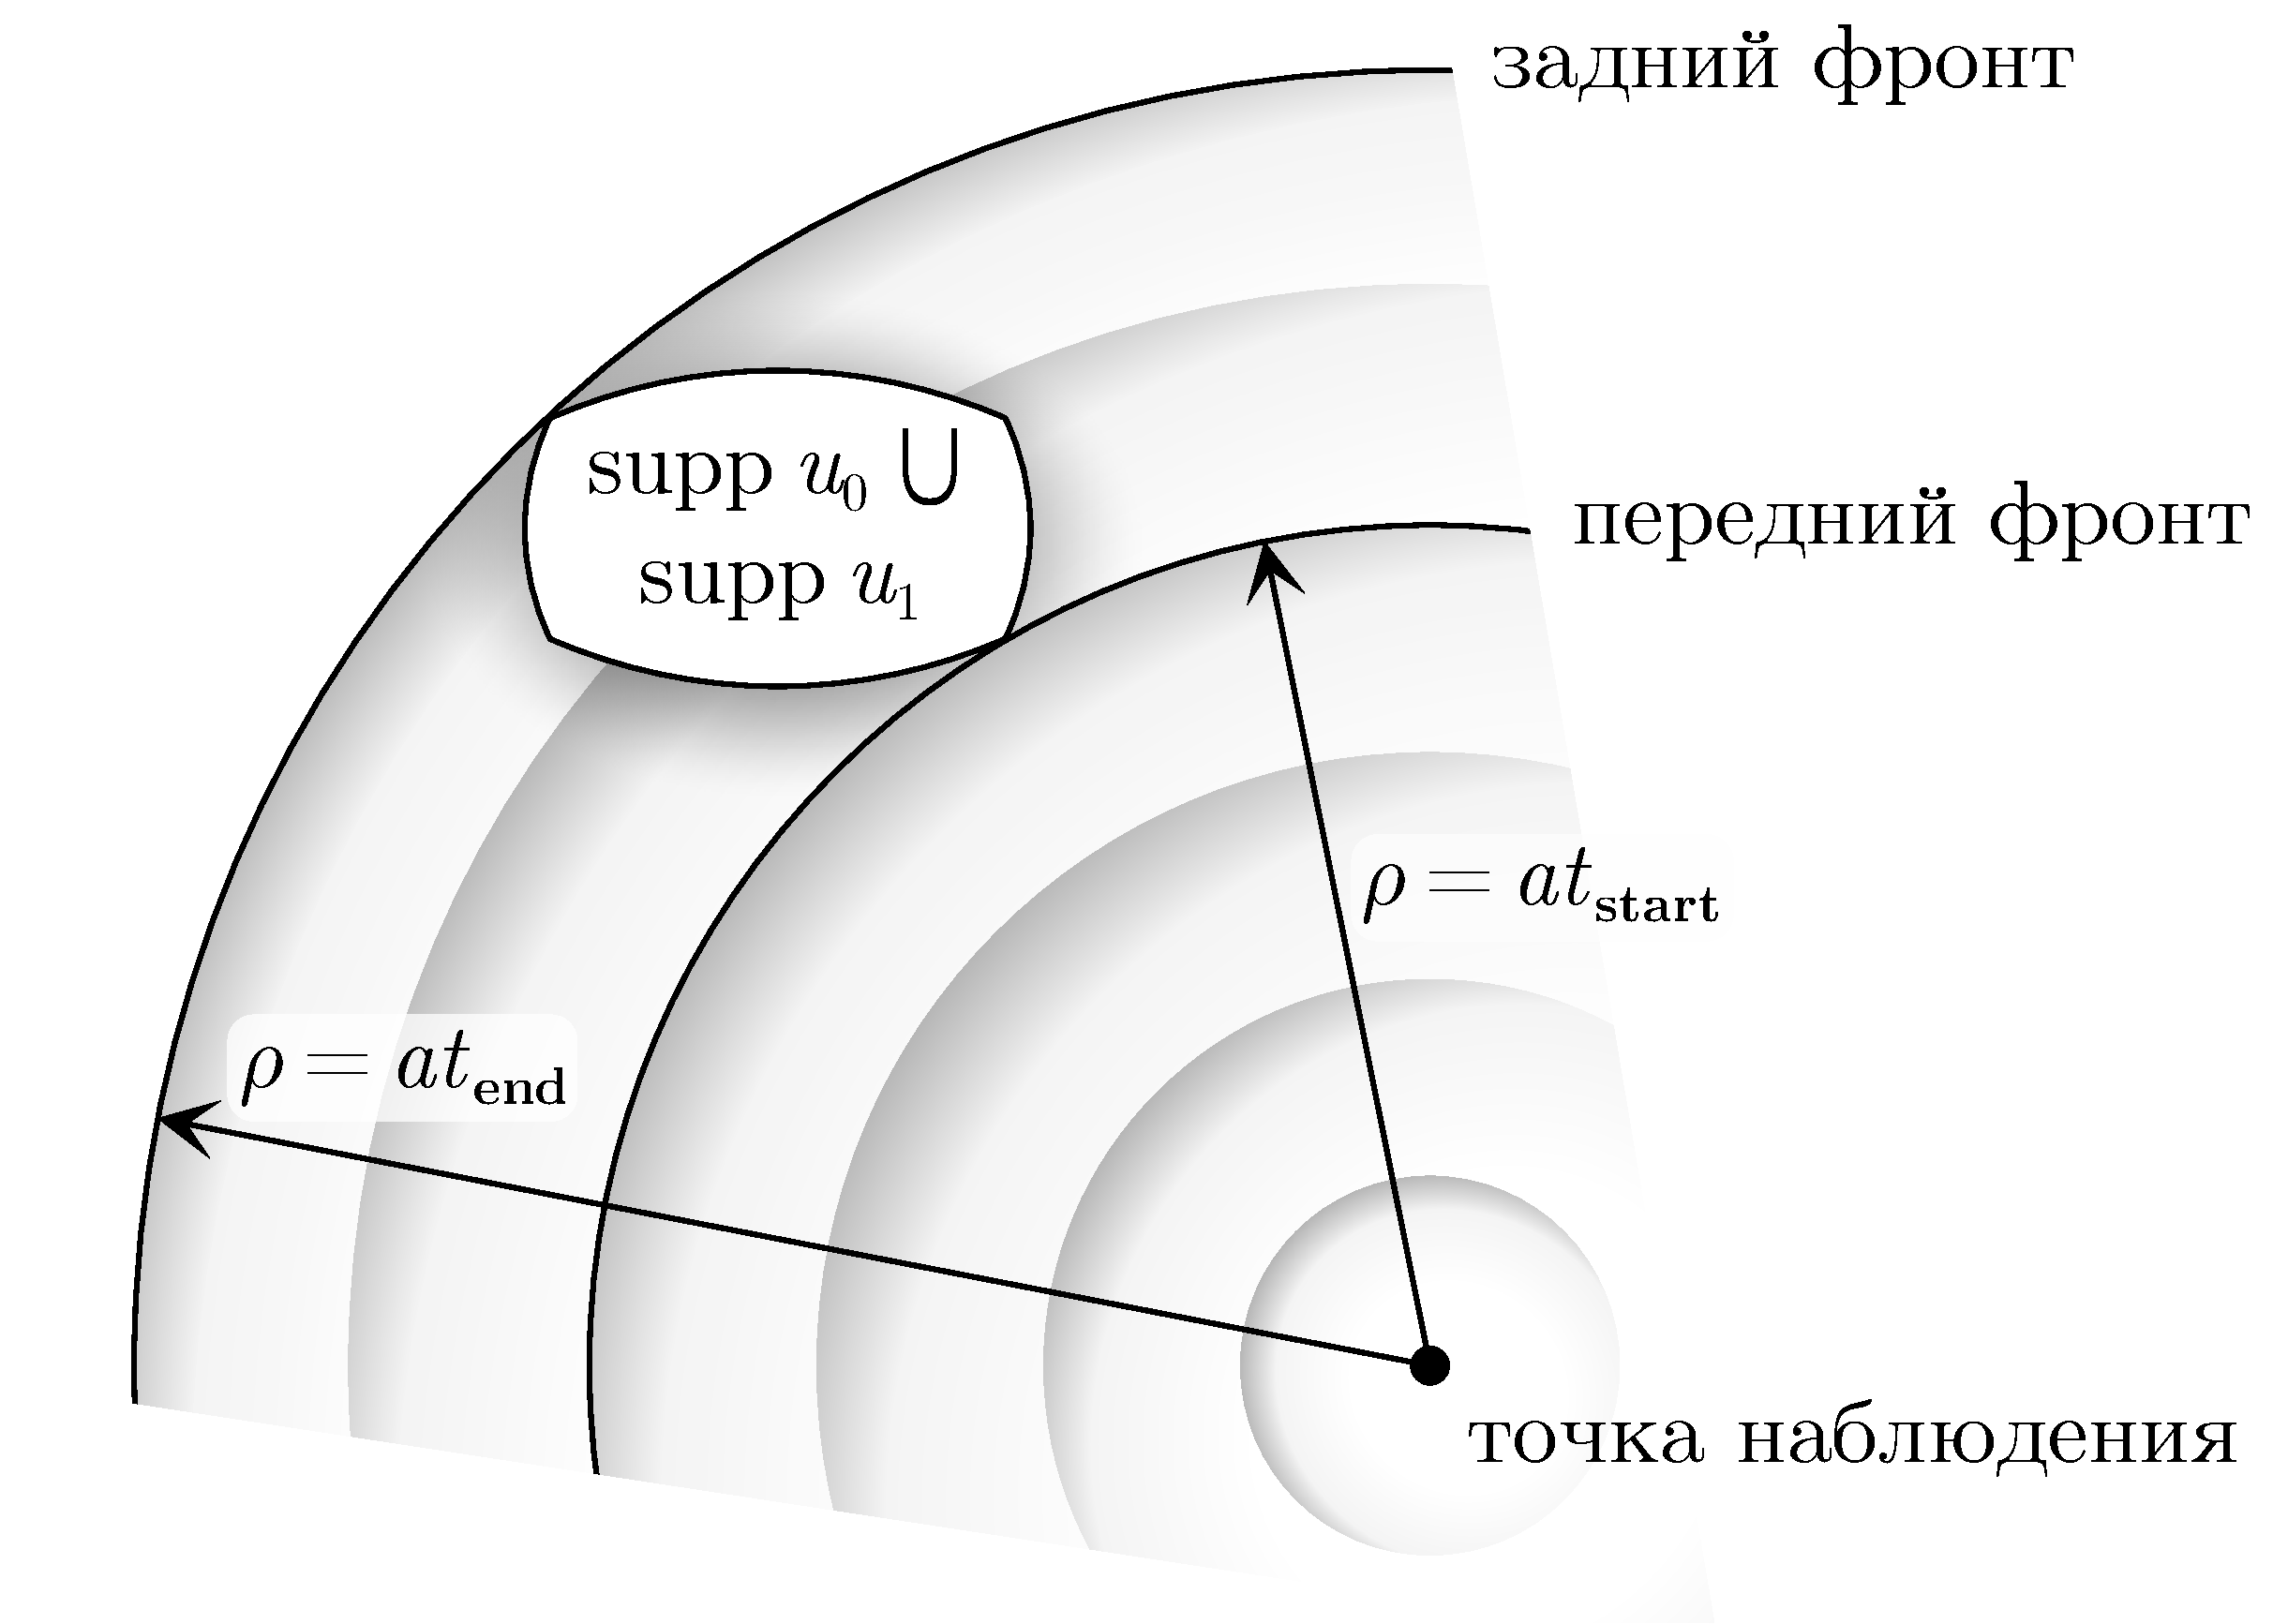
\includegraphics[width=0.45\textwidth]{./pic 7.pdf}

Значение $u(t,x_0)$ \ $\sim$ \ интеграл по сфере радиусом $|x_0 -\xi| = \rho = at$

\end{document}
\newpage
\documentclass[../main.tex]{subfiles}
\begin{document}

\section{Теорема о единственности классического решения задачи Коши для волнового уравнения (на примере случая \texorpdfstring{$\R^2$}{R\textasciicircum 2}). Метод интеграла энергии.}


\begin{theorem} Классическое решение ЗК для волнового уравнения в $\mathbb{R}^n$ единственно.
\end{theorem}
\begin{proof}[Доказательство (для случая $\R^2$)]
Пусть $u_{1}$ и $u_{2}$ - классические решения.

Тогда функция $v(x,y,t) = u_1 - u_2$ удовлетворяет полностью однородной задаче: 
$$
\begin{cases}
  v_{tt} - a^2(v_{xx} + v_{yy}) = 0\\
  v|_{t=0} = v_t|_{t=0} = 0
\end{cases}
$$
Наша цель - показать, что $v\equiv 0 $ при $ t\geq 0,\ (x,y) \in \mathbb{R}^2$.

Возьмем точку $ (x_0, y_0, t_0),\ \ t_0 > 0,\ (x,y) \in \R^2$. \; Выпустим из этой точки характеристическую поверхность --- конус:
$$ 
w(t,x) = a^2(t - t_0)^2 - (x - x_0)^2 - (y - y_0)^2 = 0,\quad t < t_0
$$
Возьмем его часть --- усечённый конус $ V_T $ с нижним основанием $ \Sigma_0 $, верхним основанием $ \Sigma_T $  и боковой поверхностью $ \Gamma_T:$
\begin{center}
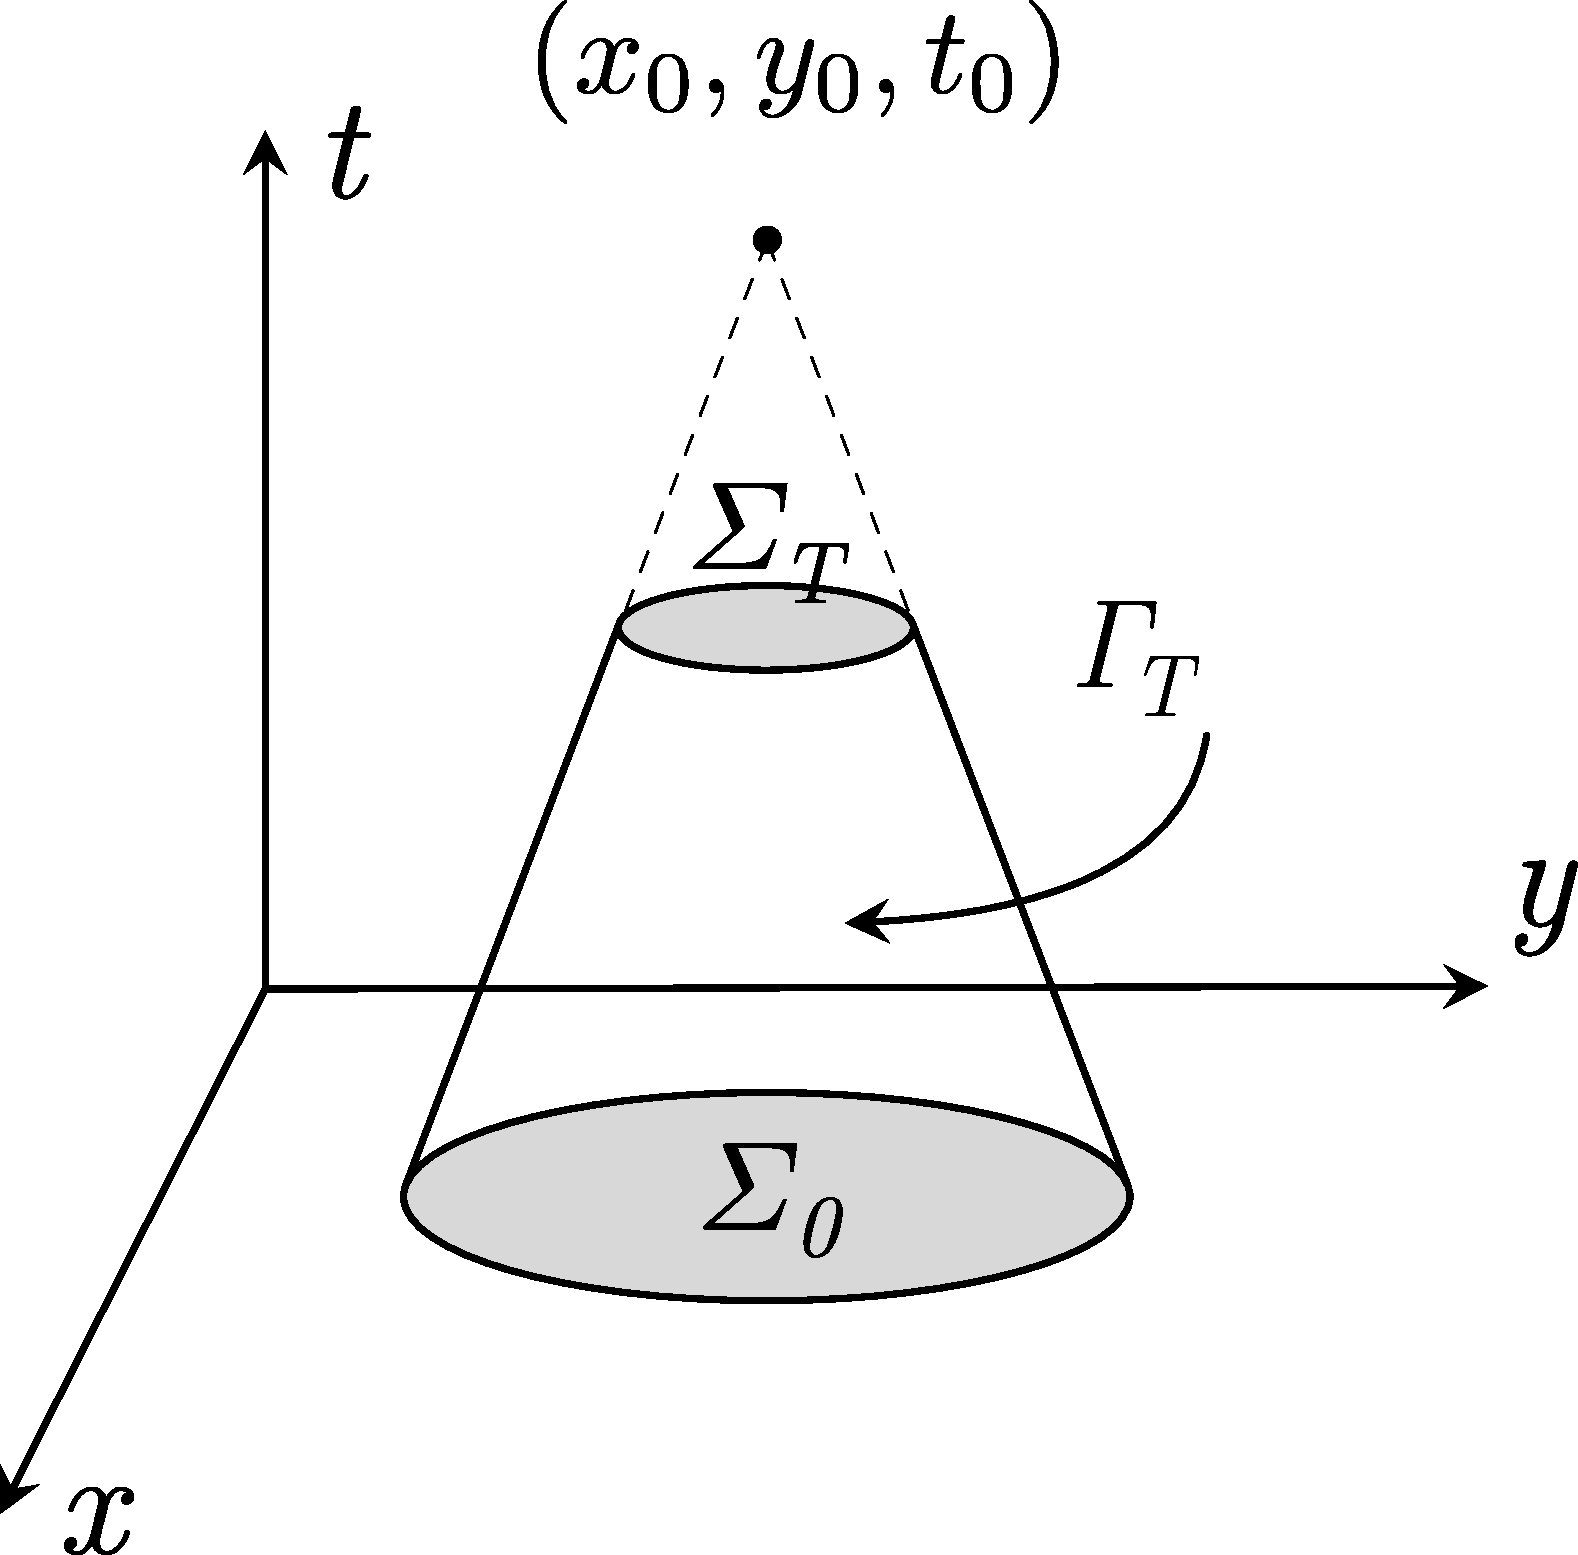
\includegraphics[width=0.28\linewidth]{./pic 8.pdf}
\end{center}
Вектор (внешней) нормали $ \vec{n} $ к этому усеченному конусу:
\begin{itemize}
	\item на $\Sigma_T:\ \vec{n} = \begin{pmatrix}1 & 0 & 0\end{pmatrix}^T $
	
	\item на $\Sigma_0:\ \vec{n} = \begin{pmatrix}-1 & 0 & 0\end{pmatrix}^T $
	
	\item на $\Gamma_T:\ \vec{n}=\dfrac{-1}{\sqrt{w_x^2+w^2_y+w^2_t}}
  \begin{pmatrix} w_x \\ w_y \\ w_t \end{pmatrix} =
  \begin{pmatrix} n_x \\ n_y \\ n_t \end{pmatrix}
  $
  \vspace{0.5em}

  В силу уравнения характеристик $\; w_t^2 - a^2w^2_x - a^2w^2_y = 0 \;$ (задаёт конус) имеем

  $n^2_t = a^2 \roundBr{n^2_x + n^2_y}$\\
  $n^2_t + n^2_x + n^2_y = 1 \quad \Rightarrow \quad n^2_t = \dfrac{a^2}{a^2 +1} \quad \Rightarrow\quad n_t = \dfrac{a}{\sqrt{a^2+1}}.$
\end{itemize}


Функция 
$ \; \psi = v_t(v_{tt}- a^2v_{xx} - a^2v_{yy})\; $ тождественно равна нулю.

Раскроем скобки:
\begin{flalign*}
  \qquad 0\;\; &= v_t v_{tt} - a^2 v_t v_{xx}-a^2 v_t v_{yy}= &&\\
  &=\frac{1}{2}\roundBr{v^2_t}_t + a^2 v_x v_{xt}-\roundBr{a^2 v_t v_x}_x + a^2 v_y v_{yt} - \roundBr{a^2 v_t v_y}_y = &&\\ 
  &=\frac{1}{2}\roundBr{v^2_t}_t - \roundBr{a v_t v_x}_x - \roundBr{a v_t v_y}_y + \roundBr{\frac{1}{2}a^2v^2_x}_t+\roundBr{\frac{1}{2}a^2v^2_y}_t = &&\\ 
  &=\roundBr{\frac{v^2_t+a^2v^2_x+a^2v^2_y}{2}}_t+\roundBr{-a^2 v_t v_x}_x + \roundBr{-a^2 v_t v_y}_y = &&\\
  &= F^{(t)}_t + F^{(x)}_x + F^{(y)}_y = \div\vec{F},
\end{flalign*}
\qquad где введено поле $\vec{F}$.
\vspace{0.7em}
% \begin{multline*}
%   0 = v_t v_{tt} - a^2 v_t v_{xx}-a^2 v_t v_{yy}= \\
%   \begin{aligned}
%   &=\frac{1}{2}(v^2_t)_t + a^2 v_x v_{xt}-(a^2 v_t v_x)_x + a^2 v_y v_{yt} - (a^2 v_t v_y)_y = \\ 
%   &=\frac{1}{2}(v^2_t)_t - (a v_t v_x)_x-(a v_t v_y)_y + \roundBr{\frac{1}{2}a^2v^2_x}_t+\roundBr{\frac{1}{2}a^2v^2_y}_t = \\ 
%   &=\roundBr{\frac{v^2_t+a^2v^2_x+a^2v^2_y}{2}}_t+(-a^2 v_t v_x)_x+(-a^2 v_t v_y)_y =
%   \end{aligned} \\
%   = F^{(t)}_t + F^{(x)}_x + F^{(y)}_y = \div \vec{F}
% \end{multline*}
% Введем в рассмотрение векторное поле $ \vec{F} = \begin{pmatrix}F^{(t)} &F^{(x)}  &F^{(y)} \end{pmatrix}^T $. Тогда то выражение, к которому мы пришли, есть
% $\div \vec{F}$.

Проинтегрируем полученную дивергенцию по объему усеченного конуса:
\begin{multline*}
  0 = \iiint\limits_{V_T}\div\vec{F} =
  \oiint\limits_{\partial V_T}(\vec{F},\vec{n})\, dS 
  =\iint\limits_{\Sigma_T}\frac{v^2_t+a^2v^2_x+a^2v^2_y}{2}\, dS - \iint\limits_{\Sigma_0}\frac{v^2_t+a^2v^2_x+a^2v^2_y}{2}\, dS + \\[0.4em]
  + \frac{1}{2}\iint\limits_{\Gamma_T}\roundBr{(v^2_t+a^2v^2_x+a^2v^2_y)n_t-2a^2v_tv_xn_x - 2a^2v_tv_yn_y}dS
  \ = \ E(\Sigma_T) - E(\Sigma_0) + E(\Gamma_T)
\end{multline*}

В силу условий $ v|_{t=0} = v_t|_{t=0} = 0$ \ имеем \ $ E(\Sigma_0)=0 $ \ (под интегралом тождественный ноль).

Тогда $ E(\Sigma_T)+E(\Gamma_T)=0 $. \ 
Кроме того, \ $ E(\Sigma_T)\geq 0 $ \ (под интегралом сумма квадратов).
\vspace{0.5em}

Покажем, что и $ E(\Gamma_T)\geq 0 $: разделим и домножим её на $ n_t=\dfrac{a}{\sqrt{a^2+1}} $
\begin{multline*}
  \frac{1}{2}\frac{\sqrt{a^2+1}}{a}\iint\limits_{\Gamma_T}\roundBr{(v^2_t+a^2v^2_x+a^2v^2_y)n^2_t \; - \; 2a^2v_tv_xn_tn_x \; - \; 2a^2v_tv_yn_tn_y} dS = \\ \shoveleft{
  =\frac{1}{2}\frac{\sqrt{a^2+1}}{a}\iint\limits_{\Gamma_T} \Bigl( v^2_t \overbrace{a^2(n^2_x + n^2_y)}^\text{= $n_t^2$}\; + \; a^2v^2_xn^2_t \; + \; a^2v^2_yn^2_t\; - \; 2a^2v_tv_xn_tn_x \; - \; 2a^2 v_t v_y n_t n_y \Bigr)\, dS }\\
  = \frac{1}{2} a \sqrt{a^2+1} \iint\limits_{\Gamma_T} \roundBr{(v_tn_x -v_xn_t)^2+(v_tn_y-v_yn_t)^2} dS \;\ \geq\ 0  
\end{multline*}

Значит,\; $ E(\Sigma_0)=E(\Sigma_T)=E(\Gamma_T)\equiv 0.$
\; Из $ E(\Sigma_T)\equiv 0 $ получаем: 
$$ v_t\equiv 0,\ v_x\equiv 0,\ v_y\equiv 0 \quad \Rightarrow \quad v = \text{const} = v|_{t=0} = 0 
$$
Это верно всюду внутри усеченного конуса.
Заметая такими конусами всё пространство, получим, что $ v \equiv 0 $.
\end{proof}
\end{document}
\newpage
\documentclass[../main.tex]{subfiles}
\begin{document}

\section{Билет 9. Формула Пуассона решения задачи Коши для однородного уравнения теплопроводности в \texorpdfstring{$\R^1$}{R}. Фундаментальное решение. Существование классического решения задачи Коши при непрерывной ограниченной начальной функции.}

\paragraph{Задача:}
\begin{equation*}
\begin{cases}
	u_t - a^2u_{xx} = 0, &x \in \R,\ t > 0 \\
	u\bigr|_{t = 0} = u_0(x), &x \in \R
\end{cases}
\end{equation*}

\subsection{Наводящие соображения}

На консультации 2021 года лектор сказал, что эту часть можно не учить. Поэтому можете сразу перейти к \hyperref[sec:FormalProof]{формальному доказательству формулы Пуассона.}
\vspace{0.7em}

Итак, пусть для начала:
\begin{equation*}
u_0(x) = \begin{cases} 
	1, &x \geq 0, \\
	0, &x < 0 
\end{cases} 
\end{equation*}
Сделаем замену: 
\begin{equation*}
\begin{cases}
	\tau = \alpha t, &\alpha > 0, \\
	\xi = \beta x, &\beta > 0.
\end{cases}
\end{equation*}
Пусть $u(t, x)$ - решение задачи. \ Введём $v(\tau, \xi) = u\left(\dfrac{\tau}{\alpha},\ \dfrac{\xi}{\beta}\right)$. \ Тогда
\begin{enumerate}
	\vspace{-0.7em} % Мне показалось, что отступ между текстом и первым элементом слишком большой. Я мог бы использовать \begin{enumerate}[topsep = 0em], но тогда отступ после последнего элемента тоже бы уменьшился
	\item $v\bigr|_{t=0} = \begin{cases} \begin{aligned}
		1, && \frac{\xi}{\beta} \geq 0 &&\Leftrightarrow && \xi \geq 0 \\
		0, && \frac{\xi}{\beta} < 0 && \Leftrightarrow && \xi < 0
	\end{aligned}\end{cases}$

	\item $v_\tau = \dfrac{1}{\alpha}u_t, \quad v_\xi = \dfrac{1}{\beta}\, u_x, \quad v_{\xi \xi} = \dfrac{1}{\beta^2}\, u_{xx} \qquad\Rightarrow\qquad \alpha v_{\tau} = a^2 \beta^2 v_{\xi \xi}$
\end{enumerate}

Функция $v$ в общем случае будет решением другой задачи Коши, но при $\alpha = \beta^2$ --- той же самой задачи Коши. Значит, решение не единственно: если $u(t,x)$ --- решение, то $\,\forall\, \beta > 0$ функция $v(t,x) = u\left(\dfrac{t}{\beta^2},\ \dfrac{x}{\beta}\right)$ --- тоже решение.

\begin{definition} 
Множество преобразований $\{u_{\alpha}\}_{\alpha \in \mathcal{D}}$ --- \emph{однопараметрическая группа преобразований,} если:
\begin{itemize}
	\item Это множество замкнуто относительно операции композиции:
	$$\forall\, \alpha, \beta \in \mathcal{D} \quad \exists!\,\gamma \in \mathcal{D}\colon \quad u_\alpha \circ u_\beta = u_\gamma$$
	
	\item Оно содержит нейтральный элемент --- тождественное преобразование:
	$$\exists!\, o \in \mathcal{D} \quad \bigl(\forall\, \alpha \in \mathcal{D} \quad u_o \circ u_\alpha = u_\alpha \circ u_o = u_\alpha \bigr)$$
	
	\item У каждого элемента есть обратный, и их композиция в любом порядке даёт тождественное преобразование.
\end{itemize}
\end{definition}
	
\begin{definition}
	Функция $I(x)$ --- \textit{инвариант однопараметрической группы преобразовний}, если $\Forall \alpha \in \mathcal{D} \quad I(x) \equiv I(u_{\alpha}(x))$
	\end{definition}
	\begin{definition}
	Говорят, что \textit{уравнение допускает однопараметрическую группу преобразований}, если все преобразования группы переводят решения этого уравнения в решения.\footnote{В прошлых версиях файла определение гласило, что уравнение допускает группу преобразований, если оно инвариантно относительно всех преобразований группы. Но непонятно, что подразумевается под инвариантностью \emph{уравнения}. Новое определение же опирается на инвариантность \emph{функций}. Оно взято с \href{https://matem.anrb.ru/bsuconf/2012/adlerv7.pdf}{этого сайта.}}
\end{definition}

\begin{definition}
Решение уравнения называется \textit{автомодельным}, если оно зависит только от инвариантов некоторой допустимой группы преобразований.
\end{definition}
\begin{example}
Множество преобразований
\begin{equation*}
\begin{cases}
	\tau = \beta^2 t, \\
	\xi = \beta x
\end{cases}
\end{equation*}
есть однопарметрическая группа преобразований, $z = \dfrac{x}{\sqrt{t}} $ --- инвариант группы.
\end{example}
Найдём автомодельное решение $u(t, x) = f\brs{\dfrac{x}{\sqrt{t}}} = f(z)$. \\
В этом случае:
\begin{equation*}
	u_t = f'\brs{\dfrac{x}{\sqrt{t}}} \cdot \brs{\frac{-x}{2t^{3/2}}} 
	\qquad u_x = f'\brs{\frac{x}{\sqrt{t}}} \cdot \frac{1}{\sqrt{t}} 
	\qquad u_{xx} = f''\brs{\frac{x}{\sqrt{t}}} \cdot \frac{1}{t}
\end{equation*}

Подставляем в уравнение:
\vspace{-0.7em}
\begin{align*}
	&-\frac{x}{2t\sqrt{t}} f'(z) = a^2 f''(z) \cdot \frac{1}{t}\\[0.3em]
	&\frac{f''(z)}{f'(z)} = - \frac{1}{a^2} \frac{x}{2\sqrt t} = -\frac{1}{2 a^2} z\\[0.2em]
	&\ln|f'(z)| = -\frac{z^2}{4a^2} + \tilde{C}_1
\end{align*}
Получили, что \ $f(z) = C_1 \displaystyle\int\limits_{-\infty}^z e^{-\frac{\eta^2}{4a^2}}\;d\eta + C_2$
\paragraph{Задача была следующей:} бесконечный стержень разделён на две половины, начальные температуры половин $T_0 = 0$ и $T_1 = 1$. Из физических соображений:
\begin{flalign*}
	& \lim\limits_{z \to - \infty} f(z) = 0 \quad \Rightarrow \quad C_2 = 0 & \\
	& \lim\limits_{z \to + \infty} f(z) = 1 \quad \Rightarrow \quad \int\limits_{-\infty}^{+\infty} e^{-\frac{\eta^2}{4a^2}}\;d \eta = C_1^{-1} = 2a \underbrace{\int\limits_{-\infty}^{+\infty} e^{-\frac{\eta^2}{4a^2}}\;d \frac{\eta}{2a}}_{\sqrt{\pi}} \quad\ \Rightarrow \quad\ C_1 = \frac{1}{\sqrt{4 \pi a^2}} &
\end{flalign*}
Окончательно:
\begin{equation*}
	f(z) = \frac{1}{\sqrt{4 \pi a^2}}\int\limits_{-\infty}^{z} e^{-\frac{\eta^2}{4a^2}}\;d \eta = \frac{2a}{\sqrt{4 \pi a^2}} \int\limits_{-\infty}^{z/2a}e^{-\mu^2}\;d \mu = \frac{1}{\sqrt{\pi}} \int\limits_{-\infty}^{z/2a}e^{-\mu^2}\;d \mu 
\end{equation*}
Введём \textbf{интеграл ошибок}:
\begin{equation*}
	\erf(z) = \frac{2}{\sqrt{\pi}} \int\limits_{0}^{z}e^{-\xi^2}\;d \xi,\; \; \erf(\pm \infty) = \pm 1,\; \; \erf(0) = 0. 
\end{equation*}
Тогда:
\begin{equation*}
	u(t, x) = f\brs{\frac{x}{\sqrt{t}}} = \frac{1}{\sqrt{\pi}} \int\limits_{-\infty}^{\frac{x}{\sqrt{4 t a^2}}} e^{-\mu^2}\;d \mu = \frac{1}{2}\sbrs{1 + \erf\brs{\frac{x}{\sqrt{4 a^2 t}}}}
\end{equation*}
\begin{enumerate}
\item Мы рассмотрим модельную задачу.
\begin{center}
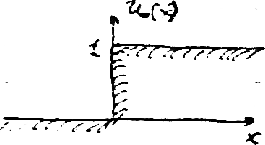
\includegraphics[width=0.2\textwidth]{9_1_new}
\end{center}
\item Увеличим ступеньку в $u_*$ раз и сдвинем.
$$u(t,x) = \frac{u_*}{2}\sbrs{1+\erf \brs{\frac{x-x_0}{\sqrt{4a^2t}}}}$$
\item Можем получить и ступеньку конечной ширины.
$$u(t,x) = \frac{u_*}{2}\sbrs{\erf \brs{\frac{x-x_1}{\sqrt{4a^2t}}}-\erf \brs{\frac{x-x_2}{\sqrt{4a^2t}}}}$$
\item Для системы из $N$ интервалов имеем:
\begin{center}
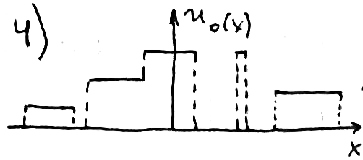
\includegraphics[width=0.2\textwidth]{9_2_new}
\end{center}
$$u(t,x) = \sum_{k=1}^{N}\frac{u_{*k}}{2}\sbrs{\erf \brs{\frac{x-x_{1k}}{\sqrt{4a^2t}}}-\erf \brs{\frac{x-x_{2k}}{\sqrt{4a^2t}}}}$$
Последнее можно переписать в следующем виде:
$$u(t,x) = \sum_{k=1}^{N}\sbrs{\frac{\fbrs{-\frac{1}{2}\erf \brs{\frac{x-x_{2k}}{\sqrt{4a^2t}}}}-\fbrs{-\frac{1}{2}\erf \brs{\frac{x-x_{1k}}{\sqrt{4a^2t}}}}}{x_{2k}-x_{1k}}}u_{*k} (x_{2k} - x_{1k})$$
\item Окончательно, пусть $u_0(x)$ финитна, непрерывна, ограничена. Разбиваем ее носитель $\mathrm{supp}\; u_0(x)$ на отрезки, аппроксимируем кусочно постоянной. Для приближенных решений справедливо:
\begin{align*}
u(t,x) &= \sbrs { \Psi (t,x, \xi) = -\frac{1}{2}\erf \brs{\frac{x - \xi}{\sqrt{4a^2t}}}} = \sum \frac{\Psi(t,x,x_{2k})-\Psi(t,x,x_{1k})}{x_{2k}-x_{1k}} u_0 \brs{\frac{x_{2k}+x_{1k}}{2}} \brs{x_{2k}-x_{1k}} \approx\\
& \approx \sum_{k=1}^N \left. \pd{\Psi}{\xi}\right |_{\xi = \frac{x_{2k}+x_{1k}}{2}} u_0 \brs{\frac{x_{2k}+x_{1k}}{2}}\brs{x_{2k}-x_{1k}} = \sbrs{\pd{\Psi}{\xi} = \frac{1}{\sqrt{4 \pi a^2 t}} e^{-\frac{(x-\xi)^2}{4a^2t}}} = \\
&= \sum_{k=1}^N \frac{1}{\sqrt{4 \pi a^2 t}} \left. e^{-\frac{(x-\xi)^2}{4a^2t}} \right |_{\xi = \frac{x_{2k}+x_{1k}}{2}} u_{*k} \brs{x_{2k} - x_{1k}} - \text{ Интегральная сумма Римана}
\end{align*}
Предположение: решение будет $$u(t,x) = \frac{1}{\sqrt{4\pi a^2 t}} \int_{-\infty}^{\infty}e^{-\frac{(x-\xi)^2}{4a^2t}} u_0(y) dy - \text{ Формула Пуассона} $$
Функция 
$$\mathcal{E}(t,x) =  \frac{1}{\sqrt{4\pi a^2 t}} e^{-\frac{x^2}{4a^2 t}} - \textbf{фундаментальное решение (или функция источника)}$$
\end{enumerate}

\subsection{Строгое доказательство}
\label{sec:FormalProof}

\begin{theorem}
Пусть $u_0\in C(\R^1),\ \abs{u_0(x)}\leq M_0\ \forall x\in \R^1$. Тогда функция $u(t,x) = \dfrac{1}{\sqrt{4\pi a^2 t}} \displaystyle\int_{-\infty}^{\infty}e^{-\dfrac{(x - y)^2}{4a^2t}} u_0(y) dy$
\begin{enumerate}
\item Принадлежит классу $C^{\infty}(t>0, x\in\R^1)\cap C(t\geq 0, x\in\R^1)$
\item Является классическим решением задачи Коши
\begin{equation*}
\begin{cases}
	u_t - a^2u_{xx} = 0, t > 0, \; x \in \R^3, \\
	u\bigr|_{t = 0} = u_0(x), \; x \in \R
\end{cases}
\end{equation*}
\item $\abs{u(t,x)}\leq M\ \forall t \geq 0,x\in\R^1$
\end{enumerate}
\end{theorem}
\begin{proof}
\begin{enumerate}
\item 
В исходном интеграле для $u(t,x)$ сделаем такую замену:
\[
\frac{y-x}{2a\sqrt{t}}=\eta ,\ y=x+2a\sqrt{t}\eta ,\ dy=2a\sqrt{t}d\eta
\]
Тогда получим
\[
u(t,x)=\frac{1}{\sqrt{\pi}}\int_{-\infty}^{\infty}e^{-\eta^2} u_0(x+2a\sqrt{t}\eta) d\eta,\ u_0(x+2a\sqrt{t}\eta)  \in C(t\geq 0, x\in\R^1,\eta\in\R^1)
\]
Оценим $\abs{e^{-\eta^2} u_0(x+2a\sqrt{t}\eta)}\leq M_0e^{-\eta^2}$, причем $\displaystyle\int_{-\infty}^{\infty}M_0e^{-\eta^2}d\eta <\infty\Rightarrow$ этот интеграл сходится абсолютно и равномерно, а значит лежит в $C(t\geq 0, x\in\R^1)$. Отсюда следует третье утверждение теоремы.

Возьмем 
\[
u_x(t, x)\sim \int_{-\infty}^{\infty}\frac{1}{4a^3\sqrt{\pi}t^{3/2}}e^{-\dfrac{(x-y)^2}{4a^2t}} (y-x)u_0(y) dy=J, 
\]
где выражение под интегралом лежит в $C(t\geq 0, x\in\R^1,\eta\in\R^1)$.
Покажем равномерную сходимость этого интеграла серией оценок:

\begin{enumerate}
\item $\abs{y-x}\geq \abs{y}-A,\ \abs{x}<A,\ y \in \R$
\item $\abs{y-x}\leq \abs{y}+A$
\item При $\abs{y}>A$ : $(y-x)^2\geq (\abs{y}-A)^2=y^2+A^2-2\dfrac{\abs{y}}{\sqrt{2}}(\sqrt{2}A)\geq y^2+A^2-\dfrac{y^2}{2}-2A^2=\dfrac{y^2}{2}-A^2$.

При $\abs{y}\leq A\ : (x-y)^2>-\dfrac{A^2}{2}$.
\item Возьмем
\[
\phi_A(y)=\begin{cases}
-\dfrac{y^2}{2}-A^2,\ &\abs{y}\geq A\\
-\dfrac{A^2}{2},\ &\abs{y}<A
\end{cases}
\]
Тогда $(x-y)^2\geq\phi_A(y) \Forall x\leq A,y \in \R$.
\end{enumerate}
Получили следующую оценку:
\[
\abs{\frac{1}{4a^3\sqrt{\pi}t^{3/2}}e^{-\dfrac{(x-y)^2}{4a^2t}} (y-x)u_0(y)}\leq \frac{M_0}{4a^3\sqrt{\pi}t^{3/2}}(\abs{y}+A)e^{-\dfrac{\phi_A(y)}{4a^2t}}
\]
Этот интеграл сходится при ограничения на $t$, т.е. в прямоугольнике $Q=\{t\in (t_1, t_2),x\in (-A, A)\}$, т.е. есть равномерная сходимость $J$ в любом прямоугольнике. Беря в качестве $Q$ всевозможные такие прямоугольники, получим $J\in C(t\geq 0, x\in\R^1)$. Аналогично будет для любой другой производной (будет асимптотика $\abs{P_n(y)}e^{-\alpha y^2}$).
\item $\ $
\[
\begin{split}
&\mathcal{E} (t, x-y)=\frac{1}{\sqrt{4\pi a^2t}}e^{-\frac{(x-y)^2}{4a^2t}}\\[7pt] 
&\mathcal{E}_x (t, x-y)=-\frac{(x-y)}{{2\sqrt{\pi} 2a^3t^{3/2}}}e^{-\frac{(x-y)^2}{4a^2t}}\\[7pt]
&\mathcal{E}_{xx} (t, x-y)=\frac{1}{2\sqrt{\pi}}\left[\frac{-1}{2a^3t^{3/2}}+\frac{(x-y)^2}{4a^5t^{5/2}} \right]e^{-\frac{(x-y)^2}{4a^2t}}\\[7pt] 
&\mathcal{E}_t (t, x-y)=\frac{1}{2\sqrt{\pi}}\left[\frac{-1}{2at^{3/2}}+\frac{(x-y)^2}{4a^3t^{5/2}} \right]e^{-\frac{(x-y)^2}{4a^2t}}
\end{split}
\]
Тогда 
\[
u_t-a^2u_{xx}=\int\limits_{-\infty}^{+\infty}\cancelto{0}{\left[\mathcal{E}_t(t, x-y)-a^2\mathcal{E}_{xx}(t, x-y) \right]}u_0(y)dy=0.
\]
Начальное условие (используя самое начало выкладок)
\[
\while{u}{t=0}=\frac{1}{\sqrt{\pi}}\int\limits_{-\infty}^{+\infty}e^{-\eta^2}u_0(x)d\eta = u_0(x)
\]
\end{enumerate}
Теорема доказана.
\end{proof}




\end{document}
\newpage
\documentclass[../main.tex]{subfiles}
\begin{document}

\section[Теорема единственности для волнового уравнения]{Теорема о единственности классического решения задачи Коши для волнового уравнения (на примере случая $\R^2$). Метод интеграла энергии.}


\begin{theorem} Классическое решение ЗК для волнового уравнения в $\mathbb{R}^n$ единственно.
\end{theorem}
\begin{proof}[Доказательство (для случая $\R^2$)]
Пусть $u_{1}$ и $u_{2}$ -- классические решения.

Тогда функция $v(x,y,t) = u_1 - u_2$ удовлетворяет полностью однородной задаче: 
$$
\begin{cases}
  v_{tt} - a^2(v_{xx} + v_{yy}) = 0\\
  \eval{v}_{t=0} = \eval{v_t}_{t=0} = 0
\end{cases}
$$
Наша цель - показать, что $v\equiv 0 $ при $ t\geq 0,\ (x,y) \in \mathbb{R}^2$.

Возьмем точку $ (x_0, y_0, t_0),\ \ t_0 > 0,\ (x,y) \in \R^2$. \; Выпустим из этой точки характеристическую поверхность -- конус:
$$ 
w(t,x) = a^2(t - t_0)^2 - (x - x_0)^2 - (y - y_0)^2 = 0,\quad t < t_0
$$
Возьмем его часть -- усечённый конус $ V_T $ с нижним основанием $ \Sigma_0 $, верхним основанием $ \Sigma_T $  и боковой поверхностью $ \Gamma_T:$
\begin{center}
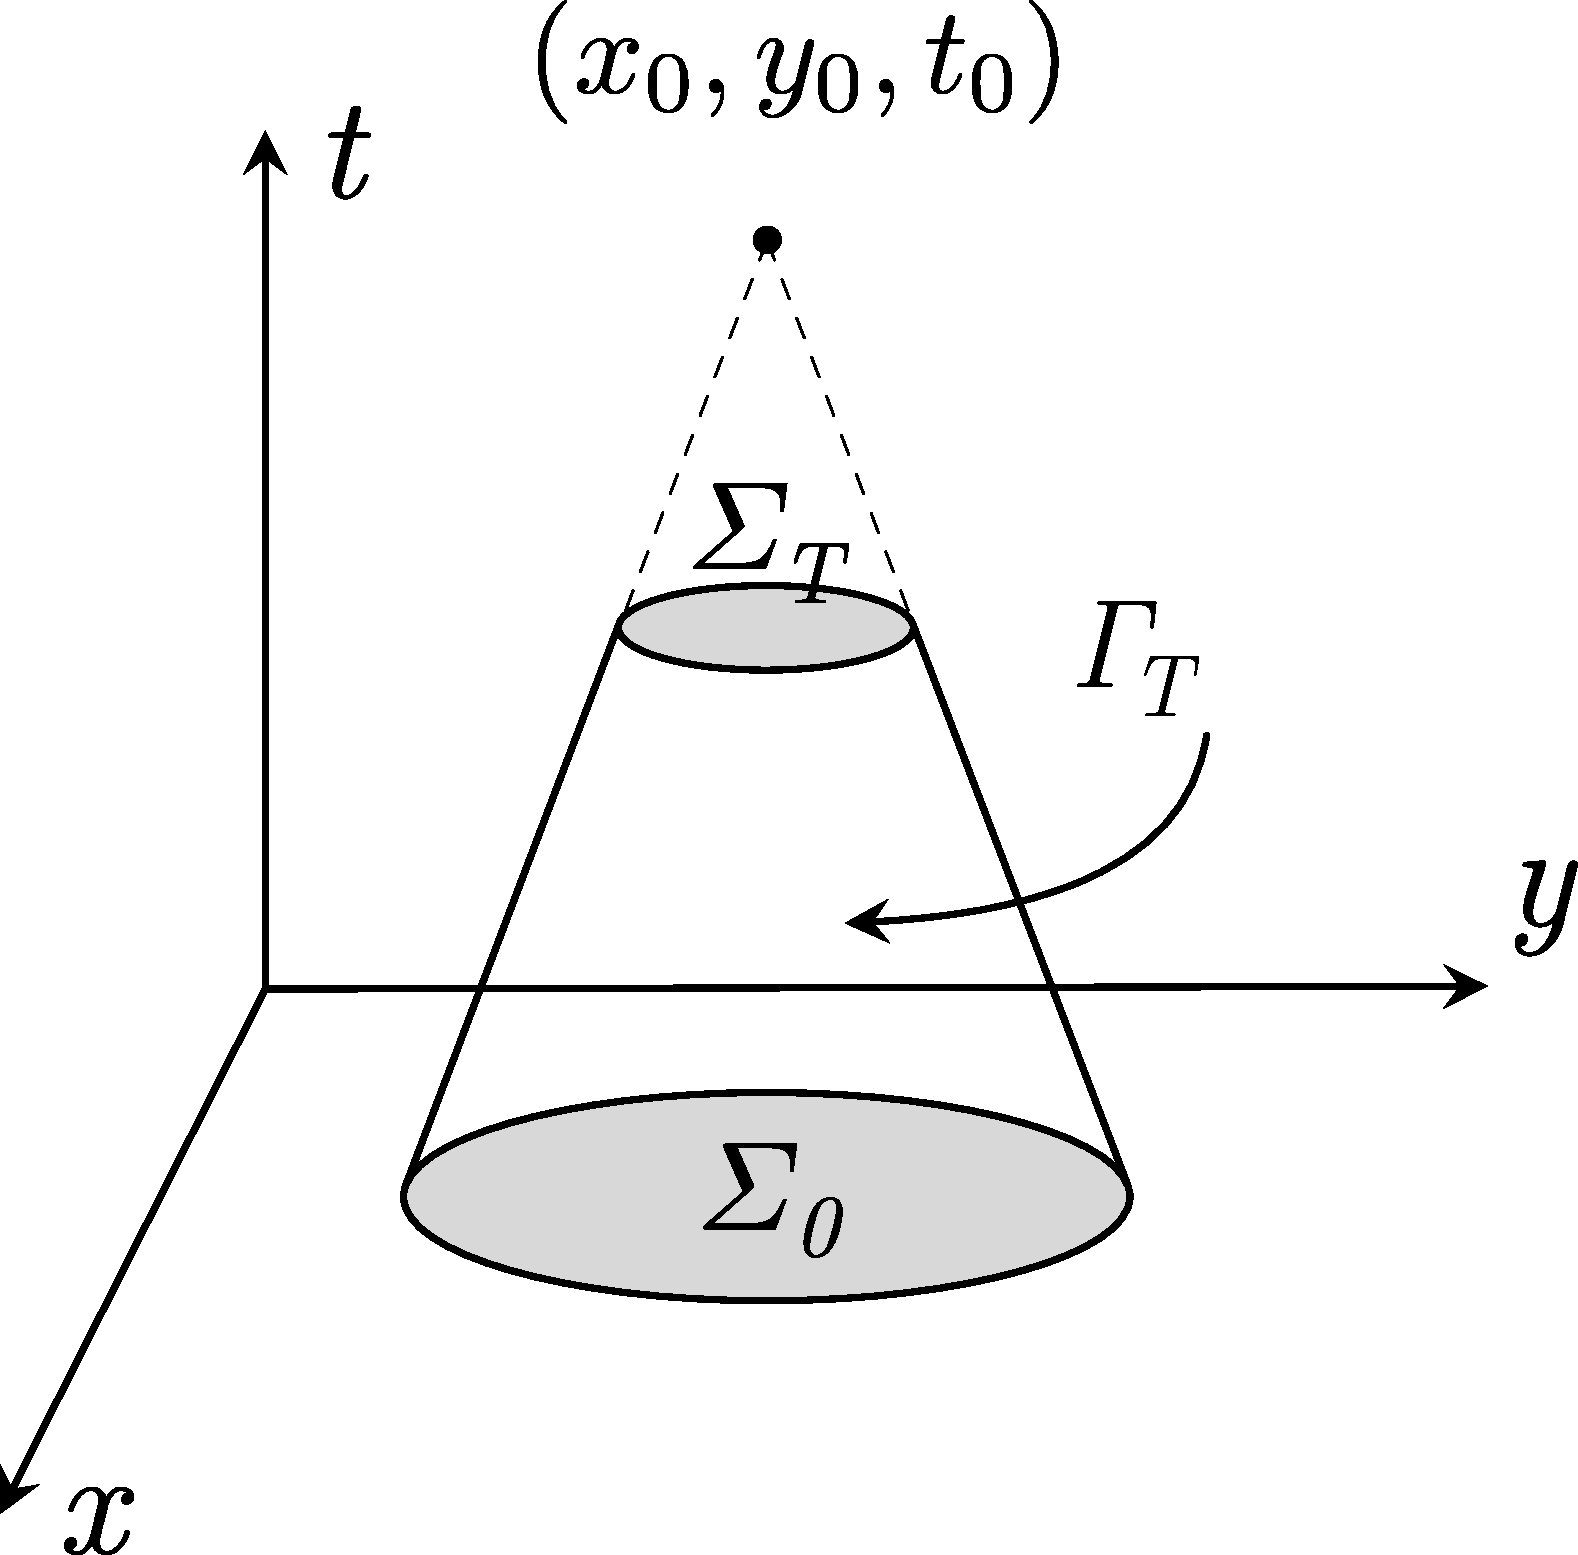
\includegraphics[width=0.28\linewidth]{./pic 10.pdf}
\end{center}
Вектор (внешней) нормали $ \vec{n} $ к этому усеченному конусу:
\begin{itemize}
	\item на $\Sigma_T:\ \vec{n} = \begin{pmatrix}1 & 0 & 0\end{pmatrix}^T $
	
	\item на $\Sigma_0:\ \vec{n} = \begin{pmatrix}-1 & 0 & 0\end{pmatrix}^T $
	
	\item на $\Gamma_T:\ \vec{n}=\dfrac{-1}{\sqrt{w_t^2+w^2_x+w^2_y}}
  \begin{pmatrix} w_t \\ w_x \\ w_y \end{pmatrix} =
  \begin{pmatrix} n_t \\ n_x \\ n_y \end{pmatrix}
  $
  \vspace{0.5em}

  В силу уравнения характеристик $\; w_t^2 - a^2w^2_x - a^2w^2_y = 0 \;$ (задаёт конус) имеем

  $n^2_t = a^2 \brk*{n^2_x + n^2_y}$\\
  $n^2_t + n^2_x + n^2_y = 1 \quad \Rightarrow \quad n^2_t = \dfrac{a^2}{a^2 +1} \quad \Rightarrow\quad n_t = \dfrac{a}{\sqrt{a^2+1}}.$
\end{itemize}


Функция \imaginarySubsection{Интеграл энергии}
$ \psi = v_t(v_{tt}- a^2v_{xx} - a^2v_{yy})\; $ тождественно равна нулю.

Раскроем скобки:
\begin{flalign*}
  \qquad 0\;\; &= v_t v_{tt} - a^2 v_t v_{xx}-a^2 v_t v_{yy}= &&\\
  &=\frac{1}{2}\brk*{v^2_t}_t + a^2 v_x v_{xt}-\brk*{a^2 v_t v_x}_x + a^2 v_y v_{yt} - \brk*{a^2 v_t v_y}_y = &&\\ 
  &=\frac{1}{2}\brk*{v^2_t}_t - \brk*{a^2 v_t v_x}_x - \brk*{a^2 v_t v_y}_y + \brk*{\frac{1}{2}a^2v^2_x}_t+\brk*{\frac{1}{2}a^2v^2_y}_t = &&\\ 
  &=\brk*{\frac{v^2_t+a^2v^2_x+a^2v^2_y}{2}}_t+\brk*{-a^2 v_t v_x}_x + \brk*{-a^2 v_t v_y}_y = &&\\
  &= F^{(t)}_t + F^{(x)}_x + F^{(y)}_y = \div\vec{F},
\end{flalign*}
\qquad где введено поле $\vec{F}$.
\vspace{0.7em}

Проинтегрируем полученную дивергенцию по объему усеченного конуса:
\begin{multline*}
  0 = \iiint\limits_{V_T}\div\vec{F}\, dV =
  \oiint\limits_{\partial V_T}(\vec{F},\vec{n})\, dS 
  =\iint\limits_{\Sigma_T}\frac{v^2_t+a^2v^2_x+a^2v^2_y}{2}\, dS - \iint\limits_{\Sigma_0}\frac{v^2_t+a^2v^2_x+a^2v^2_y}{2}\, dS + \\[0.4em]
  + \frac{1}{2}\iint\limits_{\Gamma_T}\brk*{(v^2_t+a^2v^2_x+a^2v^2_y)n_t-2a^2v_tv_xn_x - 2a^2v_tv_yn_y}dS
  \ = \ E(\Sigma_T) - E(\Sigma_0) + E(\Gamma_T)
\end{multline*}

В силу условий $ \eval{v}_{t=0} = \eval{v_t}_{t=0} = 0$ \ имеем \ $ E(\Sigma_0)=0 $ \ (под интегралом тождественный ноль).

Тогда\, $ E(\Sigma_T)+E(\Gamma_T)=0 $.\: 
Кроме того, \ $ E(\Sigma_T)\geq 0 $ \ (под интегралом сумма квадратов).
\vspace{0.5em}

Покажем, что и $ E(\Gamma_T)\geq 0 $: разделим и домножим её на $ n_t=\dfrac{a}{\sqrt{a^2+1}} $
\begin{multline*}
  \frac{1}{2}\frac{\sqrt{a^2+1}}{a}\iint\limits_{\Gamma_T}\brk*{(v^2_t+a^2v^2_x+a^2v^2_y)n^2_t \; - \; 2a^2v_tv_xn_tn_x \; - \; 2a^2v_tv_yn_tn_y} dS = \\ \shoveleft{
  =\frac{1}{2}\frac{\sqrt{a^2+1}}{a}\iint\limits_{\Gamma_T} \Bigl( v^2_t \overbrace{a^2(n^2_x + n^2_y)}^\text{= $n_t^2$}\; + \; a^2v^2_xn^2_t \; + \; a^2v^2_yn^2_t\; - \; 2a^2v_tv_xn_tn_x \; - \; 2a^2 v_t v_y n_t n_y \Bigr)\, dS }\\
  = \frac{1}{2} a \sqrt{a^2+1} \iint\limits_{\Gamma_T} \brk*{(v_tn_x -v_xn_t)^2+(v_tn_y-v_yn_t)^2} dS \;\ \geq\ 0  
\end{multline*}

Значит,\; $ E(\Sigma_0)=E(\Sigma_T)=E(\Gamma_T)\equiv 0.$
\; Из $ E(\Sigma_T)\equiv 0 $ получаем: 
$$ v_t\equiv 0,\ v_x\equiv 0,\ v_y\equiv 0 \quad \Rightarrow \quad v = \text{const} = \eval{v}_{t=0} = 0 
$$
Это верно всюду внутри усеченного конуса.
Заметая такими конусами всё пространство, получим, что $ v \equiv 0 $.
\end{proof}
\end{document}
\newpage
\documentclass[../main.tex]{subfiles}
\begin{document}

\section[Уравнение теплопроводности в \texorpdfstring{$\R^1$}{R}]{Постановка задачи Коши для уравнения теплопроводности. Формула Пуассона решения задачи Коши для однородного уравнения теплопроводности в $\R^1$. Существование классического решения задачи Коши при непрерывной ограниченной начальной функции и его свойства. Фундаментальное решение уравнения теплопроводности.}

$$\text{Задача: \ }
\begin{cases}
	u_t - a^2u_{xx} = 0, &x \in \R,\ t > 0, \\
	u\bigr|_{t = 0} = u_0(x), &x \in \R.
\end{cases} $$

\Subsection{Наводящие соображения}

На \href{https://drive.google.com/file/d/15t8c9cRmu38MEu2vC06M9binZ6IPNt1k/view?usp=sharing"}{консультации} 2021 года лектор сказал, что эту часть можно не учить. Поэтому можете сразу перейти к \hyperref[sec:FormalProof]{формальному доказательству формулы Пуассона.}
\vspace{0.7em}
% Исходная ссылка Зубова https://drive.google.com/file/d/138e2xKJtS3EVTUY8himJiMg2n9gQu96B/view 

Итак, пусть для начала:
\begin{equation*}
u_0(x) = \begin{cases} 
	1, &x \geq 0, \\
	0, &x < 0 
\end{cases} 
\end{equation*}
Сделаем замену: 
\begin{equation*}
\begin{cases}
	\tau = \alpha t, &\alpha > 0, \\
	\xi = \beta x, &\beta > 0.
\end{cases}
\end{equation*}
Пусть $u(t, x)$ - решение задачи. \ Введём $v(\tau, \xi) = u\left(\dfrac{\tau}{\alpha},\ \dfrac{\xi}{\beta}\right)$. \ Тогда
\begin{enumerate}
	\vspace{-0.7em} % Мне показалось, что отступ между текстом и первым элементом слишком большой. Я мог бы использовать \begin{enumerate}[topsep = 0em], но тогда отступ после последнего элемента тоже бы уменьшился
	\item \qquad $v\bigr|_{\tau=0} = \begin{cases} \begin{aligned}
		1, \quad && \frac{\xi}{\beta} \geq 0 &&\Leftrightarrow && \xi \geq 0 \\
		0, \quad && \frac{\xi}{\beta} < 0 && \Leftrightarrow && \xi < 0
	\end{aligned}\end{cases}$

	\item \qquad $v_\tau = \dfrac{1}{\alpha}u_t, \quad v_\xi = \dfrac{1}{\beta}\, u_x, \quad v_{\xi \xi} = \dfrac{1}{\beta^2}\, u_{xx} \qquad\Rightarrow\qquad \alpha v_{\tau} = a^2 \beta^2 v_{\xi \xi}$
\end{enumerate}

Функция $v$ в общем случае будет решением другой задачи Коши, но при $\alpha = \beta^2$ --- той же самой задачи Коши. Значит, решение не единственно: если $u(t,x)$ --- решение, то $\,\forall\, \beta > 0$ функция $v(t,x) = u\left(\dfrac{t}{\beta^2},\ \dfrac{x}{\beta}\right)$ --- тоже решение.

\begin{definition} 
Множество преобразований $\{u_{\alpha}\}_{\alpha \in \mathcal{D}}$ --- \emph{однопараметрическая группа преобразований,} если:
\begin{itemize}
	\item Это множество замкнуто относительно операции композиции:
	$$\forall\, \alpha, \beta \in \mathcal{D} \quad \exists!\,\gamma \in \mathcal{D}\colon \quad u_\alpha \circ u_\beta = u_\gamma$$
	
	\item Оно содержит нейтральный элемент --- тождественное преобразование:
	$$\exists!\, o \in \mathcal{D} \quad \bigl(\forall\, \alpha \in \mathcal{D} \quad u_o \circ u_\alpha = u_\alpha \circ u_o = u_\alpha \bigr)$$
	
	\item У каждого элемента есть обратный, и их композиция в любом порядке даёт тождественное преобразование.
\end{itemize}
\end{definition}
	
\begin{definition}
	Функция $I(x)$ --- \textit{инвариант однопараметрической группы преобразовний}, если $\Forall \alpha \in \mathcal{D} \quad I(x) \equiv I(u_{\alpha}(x))$
	\end{definition}
	\begin{definition}
	Говорят, что \textit{уравнение допускает однопараметрическую группу преобразований}, если все преобразования группы переводят решения этого уравнения в решения.\footnote{В прошлых версиях файла определение гласило, что уравнение допускает группу преобразований, если оно инвариантно относительно всех преобразований группы. Но непонятно, что подразумевается под инвариантностью \emph{уравнения}. Новое определение же опирается на инвариантность \emph{функций}. Оно взято с \href{https://matem.anrb.ru/bsuconf/2012/adlerv7.pdf}{этого сайта.}}
\end{definition}

\begin{definition}
Решение уравнения называется \textit{автомодельным}, если оно зависит только от инвариантов некоторой допустимой группы преобразований.
\end{definition}
\begin{example}
Множество преобразований
\begin{equation*}
\begin{cases}
	\tau = \beta^2 t, \\
	\xi = \beta x
\end{cases}
\end{equation*}
есть однопарметрическая группа преобразований, $z = \dfrac{x}{\sqrt{t}} $ --- инвариант группы.
\end{example}
Найдём автомодельное решение $u(t, x) = f\brk*{\dfrac{x}{\sqrt{t}}} = f(z)$. \\
В этом случае:
\begin{equation*}
	u_t = f'\brk*{\dfrac{x}{\sqrt{t}}} \cdot \brk*{\frac{-x}{2t^{3/2}}} 
	\qquad u_x = f'\brk*{\frac{x}{\sqrt{t}}} \cdot \frac{1}{\sqrt{t}} 
	\qquad u_{xx} = f''\brk*{\frac{x}{\sqrt{t}}} \cdot \frac{1}{t}
\end{equation*}

Подставляем в уравнение:
\vspace{-0.7em}
\begin{align*}
	&-\frac{x}{2t\sqrt{t}} f'(z) = a^2 f''(z) \cdot \frac{1}{t}\\[0.3em]
	&\frac{f''(z)}{f'(z)} = - \frac{1}{a^2} \frac{x}{2\sqrt t} = -\frac{1}{2 a^2} z\\[0.2em]
	&\ln|f'(z)| = -\frac{z^2}{4a^2} + \tilde{C}_1
\end{align*}
Получили, что \ $f(z) = C_1 \displaystyle \int\limits_{-\infty}^z \expT{-\frac{\eta^2}{4a^2}}\, d\eta + C_2$
\paragraph{Задача была следующей:} бесконечный стержень разделён на две половины, начальные температуры половин $T_0 = 0$ и $T_1 = 1$. Из физических соображений:
\begin{flalign*}
	& \lim\limits_{z \to - \infty} f(z) = 0 \quad \Rightarrow \quad C_2 = 0 & \\
	& \lim\limits_{z \to + \infty} f(z) = 1 \quad \Rightarrow \quad \int\limits_{-\infty}^{+\infty} \expT{-\frac{\eta^2}{4a^2}}\, d \eta = C_1^{-1} = 2a \underbrace{\int\limits_{-\infty}^{+\infty} \expT{-\frac{\eta^2}{4a^2}}\, d \frac{\eta}{2a}}_{\sqrt{\pi}} \quad\ \Rightarrow \quad\ C_1 = \frac{1}{\sqrt{4 \pi a^2}} &
\end{flalign*}
Окончательно:
\begin{equation*}
	f(z) = \frac{1}{\sqrt{4 \pi a^2}}\int\limits_{-\infty}^{z} \expT{-\frac{\eta^2}{4a^2}}\, d \eta = \frac{2a}{\sqrt{4 \pi a^2}} \int\limits_{-\infty}^{z/2a}e^{-\mu^2}\, d \mu = \frac{1}{\sqrt{\pi}} \int\limits_{-\infty}^{z/2a}e^{-\mu^2}\, d \mu 
\end{equation*}
Введём \textbf{интеграл ошибок}:
\begin{equation*}
	\erf(z) = \frac{2}{\sqrt{\pi}} \int\limits_{0}^{z}e^{-\xi^2}\, d \xi\, , \qquad \erf(\pm \infty) = \pm 1,\; \; \erf(0) = 0
\end{equation*}
Тогда:
\begin{equation*}
	u(t, x) = f\brk*{\frac{x}{\sqrt{t}}} = \frac{1}{\sqrt{\pi}} \int\limits_{-\infty}^{\frac{x}{\sqrt{4 t a^2}}} e^{-\mu^2}\, d \mu = \frac{1}{2}\brk[s]*{1 + \erf\brk*{\frac{x}{\sqrt{4 a^2 t}}}}
\end{equation*}
\begin{enumerate}
\item Мы рассмотрели модельную задачу
\begin{center}
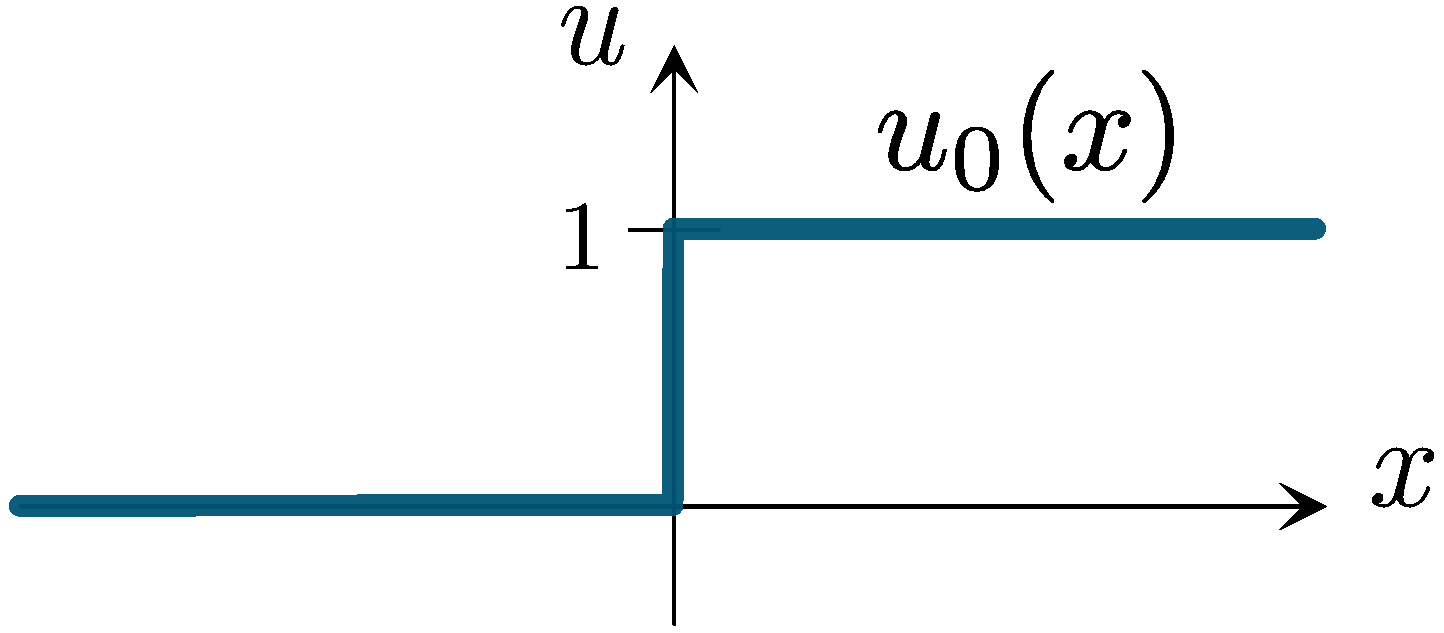
\includegraphics[height=0.11\textwidth]{./pic 11_1.pdf}
\end{center}
\item Увеличим ступеньку в $u_*$ раз и сдвинем
$$u(t,x) = \frac{u_*}{2}\brk[s]*{1+\erf \brk*{\frac{x-x_0}{\sqrt{4a^2t}}}}$$
\item Можем получить и решение для ступеньки конечной ширины:
$$u(t,x) = \frac{u_*}{2}\brk[s]*{\erf \brk*{\frac{x-x_1}{\sqrt{4a^2t}}}-\erf \brk*{\frac{x-x_2}{\sqrt{4a^2t}}}}$$
\item Для системы из $N$ интервалов имеем:
\begin{center}
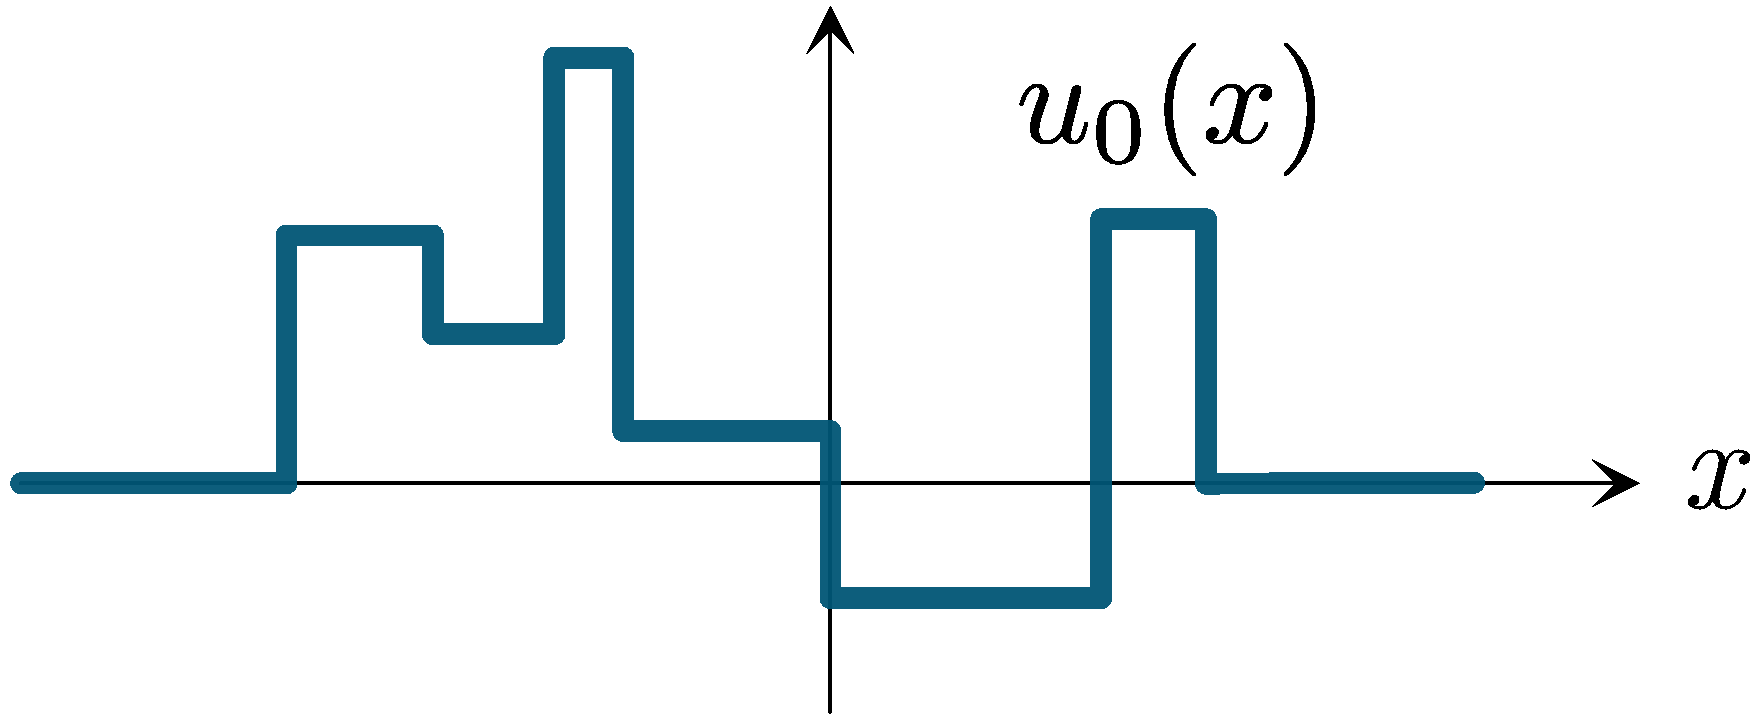
\includegraphics[height=0.125\textwidth]{./pic 11_2.pdf}
\end{center}
$$u(t,x) = \sum_{k=1}^{N}\frac{u_{*k}}{2}\brk[s]*{\erf \brk*{\frac{x-x_{1k}}{\sqrt{4a^2t}}}-\erf \brk*{\frac{x-x_{2k}}{\sqrt{4a^2t}}}}$$

Последнее можно переписать в следующем виде:
$$u(t,x) = \sum_{k=1}^{N}\brk[s]*{\frac{\brk[c]*{-\frac{1}{2}\erf \brk*{\frac{x-x_{2k}}{\sqrt{4a^2t}}}}-\brk[c]*{-\frac{1}{2}\erf \brk*{\frac{x-x_{1k}}{\sqrt{4a^2t}}}}}{x_{2k}-x_{1k}}}u_{*k} \cdot (x_{2k} - x_{1k})$$
\item Окончательно, пусть $u_0(x)$ финитна, непрерывна, ограничена. Разбиваем ее носитель $\supp u_0(x)$ на отрезки, аппроксимируем кусочно постоянной. Для приближенных решений справедливо:
\begin{align*}
u(t,x) &= \brk[s]*{
		\Psi (t,x, \xi) = -\frac{1}{2} \erf\brk*{\frac{x - \xi}{\sqrt{4a^2t}}}
		,\quad \xi_k = \frac{x_{2k} - x_{1k}}{2}
	} = \\[0.7em] 
& = \sum_{k=1}^N \frac{
		\Psi(t,x,x_{2k})-\Psi(t,x,x_{1k})
	}{x_{2k}-x_{1k}} 
	\cdot u_{*k} \cdot
	(x_{2k} - x_{1k}) \approx\\[0.7em]
& \approx \sum_{k=1}^N \eval*{ \pd{\Psi}{\xi} }_{ \xi = \xi_k } 
	u_0(\xi_k) (x_{2k} - x_{1k}) 
	= \brk[s]*{
		\pd{\Psi}{\xi} = \frac{1}{\sqrt{4 \pi a^2 t}}\, \expT{-\frac{(x-\xi)^2}{4a^2t}}
		} = \\[0.7em]
&= \sum_{k=1}^N \frac{1}{\sqrt{4 \pi a^2 t}} \eval*{
		\expT{-\frac{(x-\xi)^2}{4a^2t}}
	}_{\xi = \xi_k}
	u_0(\xi_k) (x_{2k} - x_{1k}) \text{ \ --- \ Интегральная сумма Римана}
\end{align*}

Предположение: решение будет 
$$
u(t,x) = \frac{1}{\sqrt{4\pi a^2 t}} \int_{-\infty}^{\infty} \expT{-\frac{(x-\xi)^2}{4a^2t}} u_0(\xi)\, d\xi 
\text{ \ --- \ Формула Пуассона} $$
Функция \imaginarySubsection{Фундаментальное решение}
$$\mathcal{E}(t,x) =  \frac{1}{\sqrt{4\pi a^2 t}} \expT{-\frac{x^2}{4a^2 t}} \textbf{\, ---\, фундаментальное решение (или функция источника)}$$
\end{enumerate}

\Subsection[Формула Пуассона]{Строгое доказательство} \label{sec:FormalProof} \imaginarySubsection{Свойства решения}


\begin{theorem}
Пусть $u_0\in C(\R^1),\;\; \abs*{u_0(x)}\leq M_0 \;\;\forall\, x\in \R^1.$ \ Тогда функция 
$$u(t,x) = \frac{1}{\sqrt{4\pi a^2 t}} \int_{-\infty}^{\infty} \expT{-\frac{(x - y)^2}{4a^2t}} u_0(y) dy$$
\begin{enumerate}

\item Принадлежит классу $C^{\infty}\, (t>0,\ x\in\R^1) \ \cap\ C(t \geq 0,\ x\in\R^1)$

\item Является классическим решением задачи Коши
\begin{equation*}
\begin{cases}
	u_t - a^2u_{xx} = 0, &x \in \R,\ t > 0, \\
	u\bigr|_{t = 0} = u_0(x), &x \in \R
\end{cases}
\end{equation*}

\item $\abs*{u(t,x)}\leq M \;\; \Forall t \geq 0 \Forall x\in\R^1$
\end{enumerate}
\end{theorem}


\begin{proof}
\hfill
\begin{enumerate}
\item 
В исходном интеграле для $u(t,x)$ сделаем такую замену:
\[
\frac{y-x}{\sqrt{4 a^2 t}}=\eta, 
\quad  y = x + \sqrt{4 a^2 t}\,\eta,
\quad dy = \sqrt{4 a^2 t}\, d\eta
\]
Тогда получим
\begin{multline*}
u(t,x)=\frac{1}{\sqrt{\pi}}\int_{-\infty}^{\infty}e^{-\eta^2} u_0(x+\sqrt{4 a^2 t}\, \eta)\: d\eta \\
u_0(x+\sqrt{4 a^2 t}\,\eta) 
\;\ \in \;\ C(t \geq 0,\ x \in \R^1,\ \eta \in \R^1) \hspace{8.5em}
\end{multline*}
Оценим $\abs*{e^{-\eta^2} u_0(x+\sqrt{4 a^2 t}\, \eta)}\leq M_0e^{-\eta^2}$, причем $\displaystyle\int_{-\infty}^{\infty}M_0e^{-\eta^2}d\eta$ \ сходится $\ \Rightarrow\ $ исходный интеграл сходится равномерно, а значит лежит в $C(t\geq 0,\ x\in\R^1)$. Отсюда следует третье утверждение теоремы.

\item Возьмем 
\begin{equation}
u_x(t, x)\sim \int_{-\infty}^{\infty}\frac{1}{4a^3\sqrt{\pi}t^{3/2}}\expT{-\frac{(x-y)^2}{4a^2t}} (y-x)u_0(y)\, dy
\label{eq:11:u_x}
\end{equation}
Выражение под интегралом лежит в $C(t > 0,\;\: x, y \in \R^1)$. 

Пусть $x \in [-A, A]$. Покажем равномерную сходимость интеграла серией оценок:

\begin{enumerate}

	\item При $|y|>A \colon\ $

	$(y-x)^2 \geq (|y|-A)^2
	=y^2 + A^2 - 2\dfrac{|y|}{\sqrt{2}}\brk*{\sqrt{2}A}.$

	Поскольку $2ab \leq a^2 + b^2$,

	$(y-x)^2 \geq y^2+A^2-\dfrac{y^2}{2}-2A^2=\dfrac{y^2}{2}-A^2$
	\vspace{0.3em}

	\item При $\abs*{y}\leq A \colon\ (x-y)^2 > 0$

	\item При 
	$ \forall\, y \in \R\colon\ (x-y)^2 \geq \phi_A(y) 
	= \begin{cases}
		\dfrac{y^2}{2}-A^2,\   &\abs*{y}\geq A \\
		0,\                    &\abs*{y}  <  A
	\end{cases}
	$

	\item Кроме того, $\abs*{y-x}\leq \abs*{y}+A$.
	\end{enumerate}

Получили следующую оценку (при $|x| < A$):
\[
\abs*{\frac{1}{4a^3\sqrt{\pi}t^{3/2}}\expT{-\frac{(x-y)^2}{4a^2t}} (y-x)u_0(y)}\leq \frac{M_0}{4a^3\sqrt{\pi}t^{3/2}}(\abs*{y}+A)\expT{-\frac{\phi_A(y)}{4a^2t}}
\]
Если $t \in [t_1, t_2] \subset (0, +\infty)$, то это можно ограничить выражением $C \cdot (|y| + A) \cdot \expT{\frac{\phi_A(y)}{B}},$ интеграл от которого сходится, поэтому исходный интеграл сходится равномерно.

Равномерная сходимость (по двум параметрам сразу) есть в любом прямоугольнике 
$$Q = \Bigl\{ |x| < A, \;\ t \in [t_1, t_2] \Bigr\}$$
Беря в качестве $Q$ все возможные такие прямоугольники, получим, что производная $u_x$ на всём множестве $\bigl\{ t > 0,\ x \in \R^1 \bigr\}$ существует, непрерывна и равна интегралу \eqref{eq:11:u_x}.

Аналогично будет для любой другой производной (будет асимптотика $\abs*{P_n(y)}e^{-\alpha y^2}$).
\item%
\[
\begin{split}
&\mathcal{E} (t, x-y)=\frac{1}{\sqrt{4\pi a^2t}}\,\expT{-\frac{(x-y)^2}{4a^2t}} \\[7pt]
& \mathcal{E}_x(t,x-y) = -\frac{(x-y)}{2a^2 t}\cdot \mathcal E(t,x-y) \\[7pt]
& \mathcal{E}_{xx}(t,x-y) = \brk*{-\frac{1}{2a^2 t} + \frac{(x-y)^2}{4a^4 t^2}} \mathcal E(t,x-y) \\[7pt]
& \mathcal{E}_t(t,x-y) = \brk*{-\frac{1}{2}\frac{1}{t} + \frac{(x-y)^2}{4a^2}\frac{1}{t^2}} \mathcal E(t,x-y) \\[7pt]
\end{split}
\]
Тогда 
\[
u_t-a^2u_{xx}=\int\limits_{-\infty}^{+\infty}\cancelto{0}{\left[\mathcal{E}_t(t, x-y)-a^2\mathcal{E}_{xx}(t, x-y) \right]}u_0(y)dy=0.
\]
Начальное условие (используя самое начало выкладок)
\[
\eval{u}_{t=0}=\frac{1}{\sqrt{\pi}}\int\limits_{-\infty}^{+\infty}e^{-\eta^2}u_0(x)d\eta = u_0(x)
\]
\end{enumerate}
Теорема доказана.
\end{proof}




\end{document}
\newpage
\section{Билет 12. Решение методом Фурье смешанной задачи для однородного уравнения теплопроводности на отрезке с однородными краевыми условиями Дирихле. Существование и единственность классического решения.}
% Техал Витяй
Рассмотрим смешанную (начально-краевую) задачу:
\begin{equation} \label{12_1}
	\begin{cases}
		u_t - a^2u_{xx} = f(t,x), \quad &0 < t < T, 0 < x < l, \\
		\while{u}{t=0} = u_0(x), \quad & 0 \leqslant x \leqslant l, \\
		\while{u}{x=0} = \psi_0(t), \quad \while{u}{x=l} = \psi_1(t), \quad & 0 \leqslant t \leqslant T;
	\end{cases}
\end{equation}
Рассматриваем ее классическое решение~--- функцию $u(t,x) \in C^{1,2}_{t,x}(Q_T) \cap C(\overline{Q_T})$, где \\ $Q_T = \fbrs{(t,x) : t \in (0,T); x \in (0,l)}$, удовлетворяющую в $Q_T$ уравнению, начальному и граничным условиям.
\begin{theorem}[Единственности]
	Не может существовать более одного классического решения задачи \ref{12_1}
\end{theorem}
\begin{proof}
	Если $u_1, u_2$~--- классические решения, то $v = u_1 - u_2$~--- классическое решение полностью однородной задачи. На параболической границе $\Gamma_T = \fbrs{t=0, x \in \sbrs{0,l}} \cup \fbrs{x=0, t \in \sbrs{0,T}} \cup \fbrs{x=l, t \in \sbrs{0,T}}$ $\while{v}{\Gamma_T} = 0$. Но на $\Gamma_T$ достигается максимум и минимум $v$ в $Q_T$ в силу принципа максимума $\Rightarrow v \equiv 0$
\end{proof}

Частный случай, указанный в билете:
\begin{equation*}
	\begin{cases}
		u_t - a^2u_{xx} = 0, \quad & 0 < t < T, 0 < x < l, \\
		\while{u}{t=0} = u_0(x), \quad & 0 \leq x \leq l, \\
		\while{u}{x=0} = 0, \quad \while{u}{x=l} = 0, \quad & 0 < t < T;
	\end{cases}
\end{equation*}
Из непрерывности естественно требовать выполнение условий согласования: $u_0(0) = u_0(l) = 0$. Оказывается, в таких условиях решение существует.

{\it Метод Фурье}~--- поиск решения в виде ряда по собственным функциям стационарного оператора.

Придём к этой идее. Будем искать решение $Lu = u_t - a^2u_{xx} = 0$ методом разделения переменных: \\ $u(t,x) = \Theta(t) X(x), \quad u(t,x) \not\equiv 0$.

Подставляем: $\dot{\Theta}(t) X(x) - a^2\Theta(t) X''(x) = 0 \Rightarrow \dfrac{\dot{\Theta}(t)}{a^2\Theta(t)} = \dfrac{X''(x)}{X(x)} = -\lambda = \text{const}$, т.к. равенство выполнено $\forall (t,x) \in Q_T$

Получаем на функции $\Theta$ и $X$ следующие уравнения:
\begin{equation*}
	\begin{cases}
		-X''(x) = \lambda X(x), \quad & 0 \leq x \leq l, \\
		\dot{\Theta}(t) + \lambda a^2 \Theta(t) = 0, \quad & 0 \leq t \leq T;
	\end{cases}
\end{equation*}
Из начального условия $u(t,0) = \Theta(t)X(0) \Forall t \in (0,T) \Rightarrow X(0) = 0$. Аналогично $X(l) = 0$.

Задача для $X$:
\begin{equation}
	\begin{cases}
		-X''(x) = \lambda X(x), \quad x \in (0,l), \\
		X(0) = X(l) = 0, \\
		X(x) \not\equiv 0;
	\end{cases}
\end{equation}
Поставленная задача называется {\it задачей Штурма-Лиувилля}.

Введем оператор $A$:
\begin{itemize}
	\item $\mathrm{D}(A) = \fbrs{X \in C^2[0,l] : X(0) = X(l) = 0}$
	\item $\mathrm{Im}(A) = \fbrs{Y \in C[0,l]}$
	\item $AX = -\Delta X = Y$
\end{itemize}

Задача Штурма-Лиувилля~--- это задача на собственные функции и собственные значения оператора $A$.

Решим ее:
\begin{itemize}
	\item $\lambda < 0$:

		$X(x) = C_1e^{\sqrt{\abs{\lambda}}x} + C_2e^{-\sqrt{\abs{\lambda}}x}$

			$\begin{cases}
				X(0) = C_1 + C_2 = 0, \\
				X(l) = C_1e^{\sqrt{\abs{\lambda}}l} + C_2e^{-\sqrt{\abs{\lambda}}l} = 0;
			\end{cases}$

			$\text{det}\begin{pmatrix} 1 & 1 \\ e^{2\sqrt{\abs{\lambda}}l} & 1 \end{pmatrix} = 1 - e^{2\sqrt{\abs{\lambda}}l} = 0 \Rightarrow \sqrt{\abs{\lambda}}l = 0$, противоречие.

			Итак, <<$-\Delta$>> с граничными условиями Дирихле не имеет отрицательных собственных значений.

	\item $\lambda = 0$:

		$X(x) = C_1x + C_2$

		$\begin{cases}
			X(0) = C_2 = 0, \\
			X(l) = C_1l = 0;
		\end{cases}$

		Нетривиальных решений нет.

	\item $\lambda > 0$:

		$X(x) = C_1\cos\sqrt{\lambda}x + C_2\sin\sqrt{\lambda}x$

		$\begin{cases}
			X(0) = C_1 = 0, \\
			X(l) = C_2\sin\sqrt{\lambda}l = 0;
		\end{cases}$

		$\sqrt{\lambda}l = \pi k \Rightarrow \lambda_k = \brs{\dfrac{\pi k}{l}}^2, k \in \N$

		Функции $X_k(x) = \sin\brs{\dfrac{\pi k}{l}x}$
\end{itemize}
Теперь для найденных $\lambda_k$ решаем $\dot{\Theta}_k(t) + \lambda_k a^2 \Theta_k(t) = 0 \Rightarrow \Theta_k(t) = e^{-a^2\lambda_kt}$

Мы нашли $u_k(t,x) = e^{-a^2\lambda_kt}\sin\brs{\dfrac{\pi k}{l}}$~--- счетное число бесконечно гладких решений: $u_k$ удовлетворяет задаче

\begin{equation*}
	\begin{cases}
		\brs{u_k}_t - a^2\brs{u_k}_{xx} = 0, \\
		u_k(t,0) = u_k(t,l) = 0, \\
		u_k(0,x) = X_k(x) = \sin\lambda_kx;
	\end{cases}
\end{equation*}
Тогда $u_A(t,x) = \displaystyle\sum\limits_{k=1}^N A_k u_k(t,x)$~--- решение для задачи с начальным условием $u(0,x) = \displaystyle\sum\limits_{k=1}^N A_k X_k(x)$.

Обозначим $Ku_0$~--- класс функций $u_0 = \displaystyle\sum\limits_{k=1}^N A_k X_k(x)$~--- тех, для которых умеем выписать явное решение. Пусть $A_k$~--- $k$-мерные векторы. Между $Ku_0$ и $A_k$ есть биекция (по $u_0 = \displaystyle\sum\limits_{k=1}^N A_k X_k(x)$ однозначно восстанавливаем $A_k = \dfrac{2}{l}\displaystyle\int\limits_0^l u_0(x) \sin\brs{\dfrac{\pi k}{l}x}dx$)

Бесконечномерный вектор подойдет уже не всегда. Как минимум ряд $\displaystyle\sum\limits_{k=1}^\infty A_k X_k(x)$ должен сойтись в замыкании области. Функция $\displaystyle\sum\limits_{k=1}^\infty A_k u_k(t,x)$ должна быть нужной гладкости, а также удовлетворять уравнению \ref{12_1}.

\begin{statement}
	$\fbrs{A_k}_{k=1}^{+\infty}: \displaystyle\sum\limits_{k=1}^{+\infty} \abs{A_k} < +\infty$ подойдет
\end{statement}

\begin{proof}
	Пусть $u_0(x) = \displaystyle\sum\limits_{k=1}^{+\infty} A_k\sin\brs{\dfrac{\pi k}{l}x}, \displaystyle\sum\limits_{k=1}^{+\infty} \abs{A_k} < +\infty$. Тогда $\abs{A_k\sin\brs{\dfrac{\pi k}{l}x}} \leqslant \abs{A_k} \Rightarrow$ по теореме Вейерштрасса ряд сходится абсолютно и равномерно $\Rightarrow$ сумма непрерывна.

	Равномерно сходящийся ряд можно почленно интегрировать $\Rightarrow$ по $u_0(x)$ восстанавливаем $A_n$: $\displaystyle\int\limits_0^l u_0(x)\sin\brs{\dfrac{\pi n}{l}x}dx = \displaystyle\sum_{k=1}^{+\infty} A_k \displaystyle\int\limits_0^l \sin\brs{\dfrac{\pi k}{l}x} \sin\brs{\dfrac{\pi n}{l}x} dx \Rightarrow A_n = \dfrac{2}{l} \displaystyle\int\limits_0^l u_0(x) \sin\brs{\dfrac{\pi n}{l}x} dx$

	Теперь рассмотрим ряд $u_A(t,x) \sim \displaystyle\sum\limits_{k=1}^{+\infty} A_k e^{-\brs{\frac{a\pi k}{l}}^2t} \sin\brs{\dfrac{\pi k}{l}x}$

	Пока не можем поставить знак равенства, поскольку еще не выяснили сходимость.

	$\abs{A_k e^{-\brs{\frac{a\pi k}{l}}^2t} \sin\brs{\dfrac{\pi k}{l}x}} \leqslant \abs{A_k} \Rightarrow$ ряд сходится абсолютно и равномерно, и мы можем поставить знак равенства:

	$u_A(t,x) = \displaystyle\sum\limits_{k=1}^{+\infty} A_k e^{-\brs{\frac{a\pi k}{l}}^2t} \sin\brs{\dfrac{\pi k}{l}x}$

	Покажем, что получилась $u_A(t,x) \in C^\infty(t>0, 0 \leqslant x \leqslant l)$. 

	Возьмем прямоугольник $Q_\delta = \fbrs{(t,x) : t \geqslant \delta > 0, 0 \leqslant x \leqslant l}$. 

	Формально $\dfrac{\partial u_A}{\partial t} \sim -\displaystyle\sum\limits_{k=1}^{+\infty} A_k\brs{\dfrac{a\pi k}{l}}^2 e^{-\brs{\frac{a\pi k}{l}}^2t} \sin\brs{\dfrac{\pi k}{l}x} = -\displaystyle\sum\limits_{k=1}^{+\infty} \varphi_k(t,x)$

	Для краткости введём $y = \brs{\dfrac{a\pi k}{l}}^2$.

	Оценка: $\abs{\varphi_k} \leqslant \abs{A_k}ye^{-y\delta} = \abs{A_k} \dfrac{1}{\delta} (y\delta) e^{-y\delta} \leqslant \abs{A_k} \dfrac{1}{\delta e}$

	Последнее неравенство следует из того, что функция $xe^{-x}$ имеет максимум в точке $x = 1$, равный $\dfrac{1}{e}$.

	Итак, по теореме Вейерштрасса, ряд сходится абсолютно и равномерно.

	Варьируя $\delta$, прямоугольниками $Q_\delta$ заметаем всю область $\fbrs{t > 0, 0 \leqslant x \leqslant l}$

	Для остальных производных получим то же самое~--- всегда будет получаться произведение многочлена на экспоненту с отрицательным показателем.

	Мы научились решать задачу для $u_0(x) = \displaystyle\sum\limits_{k=1}^{+\infty} A_k \sin\brs{\dfrac{\pi k}{l}x}$.
\end{proof}
\newpage
Докажем серию лемм.
\begin{lemma}
	Пусть в гильбертовом пространстве $\mathcal{H}$ оператор $A$ симметричный (самосопряжённый), т.е. $(Ax,y) = (x,Ay)$. Тогда:
	\begin{enumerate}
		\item Все собственные значения $A$ вещественны;
		\item Собственные функции, отвечающие различным собственным значениям, ортогональны.
	\end{enumerate}
\end{lemma}
\begin{proof}
	Пусть $x_k$~--- собственный вектор, отвечающий собственному значению $\lambda_k$, а $x_n$~--- собственный вектор, отвечающий собственному значению $\lambda_n$, причем $\lambda_k \not= \lambda_n$. Тогда:
	\begin{enumerate}
		\item $\lambda_k(x_k, x_k) = (Ax_k, x_k) = (x_k, Ax_k) = (x_k, \lambda_kx_k) = \overline{\lambda_k}(x_k, x_k) \Rightarrow \lambda_k = \overline{\lambda_k} \Rightarrow \mathrm{Im} \, \lambda_k = 0$
		\item $\lambda_k(x_k, x_n) = (Ax_k, x_n) = (x_k, Ax_n) = \overline{\lambda_n}(x_k,x_n) \underset{\text{пункт 1}}{=} \lambda_n(x_k,x_n) \Rightarrow \underset{\not= 0}{\underline{(\lambda_k - \lambda_n)}}(x_k,x_n) = 0 \Rightarrow (x_k,x_n) = 0$
	\end{enumerate}
\end{proof}
\begin{lemma}
	Оператор $A = -\dfrac{d^2}{dx^2}$, определенный на $\mathrm{D}(A)$, является симметричным относительно скалярного произведения в $\mathbb{L}_2\brs{[0,l]}: (u,v) = \displaystyle\int\limits_0^l u(x) \overline{v(x)} dx$
\end{lemma}
\begin{proof}
	$(Au,v) = \displaystyle\int\limits_0^l (-u''(x))\overline{v(x)}dx = \underset{= 0, \text{ в силу определения $\mathrm{D}(A)$}}{\underline{\left.-u'(x)\overline{v(x)}\right|_0^l}} + \displaystyle\int\limits_0^l u'(x) \overline{v'(x)} dx = \underset{= 0, \text{ в силу определения $\mathrm{D}(A)$}}{\underline{\left.u(x)\overline{v'(x)}\right|_0^l}} + \displaystyle\int\limits_0^l u(x)\brs{-\overline{v''(x)}}dx = (u, Av)$
\end{proof}
\begin{lemma}
	Пусть $\fbrs{e_k}$~--- не более чем счетная ортогональная система в линейном пространстве со скалярным произведением: $(e_k, e_j) = \delta_{kj} \underset{>0}{\underline{(e_k, e_k)}}$. Тогда $\forall f$ из этого пространства справедливо неравенство Бесселя: $\displaystyle\sum\limits_{k=1}^{+\infty} \abs{c_k}^2 (e_k, e_k) = \displaystyle\sum\limits_{k=1}^{+\infty} \abs{\dfrac{(f,e_k)}{(e_k,e_k)}}^2 (e_k, e_k) \leq (f, f)$
\end{lemma}
\begin{proof}
	$0 \leq \brs{f - \displaystyle\sum\limits_{k=1}^n c_ke_k, f - \displaystyle\sum\limits_{k=1}^n c_ke_k} = (f,f) - \displaystyle\sum\limits_{k=1}^n c_k(e_k,f) - \displaystyle\sum\limits_{j=1}^n \overline{c_j} (f,e_j) + \displaystyle\sum\limits_{k=1}^n \displaystyle\sum\limits_{j=1}^n c_k \overline{c_j} (e_k, e_j) = \\ = (f,f) - \displaystyle\sum\limits_{k=1}^n c_k \overline{c_k} (e_k, e_k) - \displaystyle\sum\limits_{j=1}^n c_j \overline{c_j} (e_j, e_j) + \displaystyle\sum\limits_{i=1}^n c_i \overline{c_i} (e_i, e_i) = (f,f) - \displaystyle\sum\limits_{k=1}^n \abs{c_k}^2 (e_k, e_k)$. Переходя к пределу при $n \to +\infty$, получаем $\displaystyle\sum\limits_{k=1}^{+\infty} \abs{c_k}^2 (e_k, e_k) \leq (f,f)$.
\end{proof}
\begin{lemma}
	Пусть два ряда $\displaystyle\sum\limits_{k=1}^{+\infty} \abs{\alpha_k}^2 = A, \: \displaystyle\sum\limits_{k=1}^{+\infty} \abs{\beta_k}^2 = B$ сходятся. Тогда ряд $\displaystyle\sum\limits_{k=1}^{+\infty} \alpha_k \beta_k$ сходится абсолютно, причем $\displaystyle\sum\limits_{k=1}^{+\infty} \abs{\alpha_k \beta_k} \leq \sqrt{A} \sqrt{B}$
\end{lemma}
\begin{proof}
	$\displaystyle\sum\limits_{k=1}^{n} \abs{\alpha_k \beta_k} \underset{\text{КБШ}}{\leq} \sqrt{\displaystyle\sum\limits_{k=1}^{n} \abs{\alpha_k}^2} \sqrt{\displaystyle\sum\limits_{k=1}^{n} \abs{\beta_k}^2}$. Переходя к пределу при $n \to +\infty$, получаем требуемое.
\end{proof}
\begin{lemma}
	Пусть $v(x) \in C^1\brs{[0,l]}, v(0) = v(l) = 0$. 

	Тогда ряд $\displaystyle\sum\limits_{k=1}^{+\infty} A_k \sin\brs{\dfrac{\pi k}{l}x}$, где $A_k = \dfrac{2}{l}\displaystyle\int\limits_0^l v(y)\sin\brs{\dfrac{\pi k}{l}y}dy$, сходится на $[0,l]$ к $v(x)$ абсолютно и равномерно.
\end{lemma}
\begin{proof}
	\begin{enumerate}
		\item Система $\fbrs{e_k} = \fbrs{\sin\brs{\dfrac{\pi k}{l}x}}$ ортогональна относительно скалярного произведения в $\mathbb{L}_2\brs{[0,l]}$, так как состоит из собственных функций оператора <<$-\Delta$>> с однородными условиями Дирихле~--- симметричного в $\mathbb{L}_2\brs{[0,l]}$ оператора.
		\item $A_k = \dfrac{(v,e_k)}{(e_k,e_k)},$ ряд $\displaystyle\sum\limits_{k=1}^{+\infty} \abs{A_k}^2 < +\infty$ по неравенству Бесселя.
		\item $A_k = \underset{=0}{\underline{-\left.\dfrac{2}{l} \dfrac{l}{\pi k} v(y) \cos\brs{\dfrac{\pi k}{l}y}\right|_0^l}} + \dfrac{2}{l} \dfrac{l}{\pi k} \displaystyle\int\limits_0^l v'(y) \cos\brs{\dfrac{\pi k}{l}y}dy = \dfrac{l}{\pi k} \alpha_k$, где $\alpha_k = \dfrac{2}{l} \displaystyle\int\limits_0^l v'(y) \cos\brs{\dfrac{\pi k}{l}y}dy$.
		\item Ряд $\displaystyle\sum\limits_{k=1}^{+\infty} \abs{\alpha_k}^2 < +\infty$ по неравенству Бесселя, т.к. система $\fbrs{g_k} = \fbrs{\cos\brs{\dfrac{\pi k}{l}x}}$ ортогональна относительно скалярного произведения в $\mathbb{L}_2\brs{[0,l]}$, так как состоит из собственных функций оператора <<$-\Delta$>> с однородными условиями Неймана~--- симметричного в $\mathbb{L}_2\brs{[0,l]}$ оператора.

		Ряд $\displaystyle\sum\limits_{k=1}^{+\infty} \dfrac{1}{k^2} = \dfrac{\pi^2}{6}$ сходится. Тогда сходится абсолютно ряд $\displaystyle\sum\limits_{k=1}^{+\infty} \dfrac{\alpha_k}{k} \Rightarrow \displaystyle\sum\limits_{k=1}^{+\infty} \abs{A_k} < +\infty$. 

		Функция $\varphi(x) = \displaystyle\sum\limits_{k=1}^{n} A_k \sin\brs{\dfrac{\pi k x}{l}}$ непрерывна.
		\item Сходимость к $v(x)$: Построим
			\begin{equation*}
				\tilde{v}(x) = \begin{cases} v(x), & x \in [0,l] \\ -v(-x), & x \in [-l,0] \end{cases}
			\end{equation*}
			Затем продолжим на $\R$, сделав периодической: $\tilde{v}(x+2l) = \tilde{v}(x)$.
			Получаем непрерывную периодическую функцию, а во всех точках $x \in [0,l] \exists \tilde{v}'_-(x), \tilde{v}'_+(x)$. Тогда ряд Фурье этой функции сходится к ней на всей $\R$. В силу нечетности $\tilde{v}$, этот ряд~--- только по синусам, а коэффициенты Фурье равны $A_k$ (для них совпадают формулы). Значит, на $[0,l]$ имеем $v(x) = \displaystyle\sum\limits_{k=1}^{+\infty} A_k \sin\brs{\dfrac{\pi k}{l}x}$
	\end{enumerate}
\end{proof}
Таким образом, доказана теорема:
\begin{theorem}
	Пусть в смешанной задаче
	\begin{equation*}
		\begin{cases}
			u_t - a^2u_{xx} = 0, \quad & 0 < t < T, 0 < x < l, \\
			\while{u}{t=0} = u_0(x), \quad & 0 \leq x \leq l, \\
			\while{u}{x=0} = \while{u}{x=l} = 0, \quad & 0 \leq t \leq T;
		\end{cases}
	\end{equation*}
	функция $u_0(x)$ удовлетворяет условиям гладкости $\brs{u_0 \in C^1\brs{[0,l]}}$ и согласования $\brs{u_0(0) = u_0(l) = 0}$. Тогда ряд $\displaystyle\sum\limits_{k=1}^{+\infty} A_k e^{-\brs{\frac{a\pi k}{l}}^2t} \sin\brs{\dfrac{\pi k}{l}x} = u(t,x)$, где $A_k = \dfrac{2}{l} \displaystyle\int\limits_0^l u_0(x) \sin\brs{\dfrac{\pi k}{l}x} dx$, сходится абсолютно и равномерно в $\overline{Q_T} = [0,T] \times [0,l]$, функция $u(t,x) \in C(\overline{Q_T}) \cap C^{\infty}(Q_T)$ и является классическим решением этой задачи, а любая производная при $t > 0$ от $u(t,x)$ может быть найдена почленным дифференцированием.
\end{theorem}
\newpage
\documentclass[../main.tex]{subfiles}
\begin{document}


\section{Билет 13. Метод Фурье решения смешанной задачи для уравнения колебаний струны с закреплёнными концами. Обоснование метода для случая однородного уравнения.}
% Набрано Шлёнским Владиславом
\subsection{Формулировка задачи}
\textbf{Задача:}
\begin{equation}
\label{eq:13_1}
\begin{cases}
	u_{tt} - a^2u_{xx} = f(x, t),\; (t, x) \in Q_{T} = (0, T) \times (0, l), \\
    u\bigr|_{t = 0} = u_{0}(x);\; u_{t}\bigr|_{t =0} = u_{1}(x),\; x \in [0, l], \\
    u\bigr|_{x = 0} = \psi_{0}(t),\; u\bigr|_{x = l} = \psi_{1}(t);\; t \in [0, T].
\end{cases}
\end{equation}
Рассматриваем её \textit{классическое решение} - функцию $u(t, x) \in C^{2}\bigl(Q_{T}\bigr) \cap C^{1}\bigl(\overline{Q}_{T}\bigr)$, удовлетворяющую уравнению, начальным и граничным условиям. \\
\subsection{Теорема единственности}
\begin{theorem}[Единственности]
Не может существовать более одного классического решения задачи ~\ref{eq:13_1}.
\end{theorem}
\begin{proof}
\paragraph{Единственность решения.}
Для двух решений $\tilde{u}_{1}$ и $\tilde{u}_{2}$  построим $V(t, x) = \tilde{u}_{1} - \tilde{u}_{2} \in C^{2}\bigl(Q_{T}\bigr) \cap C^{1}\bigl(\overline{Q}_{T}\bigr)$.\\$V$ - решение полностью однородной задачи:
\begin{equation*}
\begin{cases}
V_{tt} - a^2V_{xx} = 0, \\
V\bigr|_{t = 0} = V_t\bigr|_{t = 0} = 0, \\
V\bigr|_{x = 0} = V\bigr|_{x = l} = 0.
\end{cases}
\end{equation*}
Докажем, что $V \equiv 0$ с помощью интеграла энергии: рассмотрим функцию $I = V_{t}\bigl[V_{tt} - a^2V_{xx}\bigr],\; (t, x) \in Q_{T}$.
\begin{equation*}
I = V_{t}V_{tt} - a^2V_{t}V_{xx} = \dfrac{1}{2}\bigl(V_{t}^{2}\bigr)_{t} - a^2\bigl(V_{t}V_{x}
\bigr)_{x} + a^2\underbrace{V_{x}V_{xt}}_{\frac{1}{2} \bigl(V_{x}^{2}\bigr)_{t}} = \underbrace{\biggl(\dfrac{V_{t}^2 + a^2V_{x}^{2}}{2}\biggr)_{t}}_{F^1_t}  \underbrace{ - \bigl(a^{2}V_{t}V_{x}\bigr)_{x}}_{F_{x}^{2}}\; \biggr|\; \div\vec{F} = \div \begin{pmatrix}
F^1 \\
F^2
\end{pmatrix}
\end{equation*}
Воспользуемся формулой Грина: $\iint\limits_{\Omega}\bigl(\dfrac{\partial Q}{\partial x} - \dfrac{\partial P}{\partial y}\bigr)\;dxdy = \oint\limits_{\partial \Omega}Q\;dy + P\;dx$.
Для её использования требуется непрерывность производных до границы, поэтому напишем её для области: $Q_{\tau, \varepsilon} = \{(t, x)\colon\; \varepsilon < t < \tau,\; \varepsilon < x < l - \varepsilon\}$.\\
\ \\
\begin{minipage}[c]{0.2\textwidth}
\begin{center}
\begin{tikzpicture}[scale=0.55]
  \tikzstyle{axes}=[]
  \tikzstyle{important line}=[very thick]
  \tikzstyle{information text}=[rounded corners,fill=red!10,inner sep=1ex]

   \begin{scope}[style=axes]
    \draw[->] (-0.2,0) -- (5,0) node[right] {$x$};
    \draw[->] (0,-0.2) -- (0,4) node[left] {$t$};
    \end{scope}

    \coordinate [label = {below: $\varepsilon$}] (A) at (0.5, 0);
    \coordinate [label = {left: $\varepsilon$}] (B) at (0, 0.5);
    \coordinate (C) at (0.5, 0.5);

    \draw [dashed] (A) -- (C) -- (B);

    \coordinate [label = {below: $l-\varepsilon$}] (D) at (3, 0);
    \coordinate (D1) at (3, 0.5);

    \draw [dashed] (D) -- (D1);

    \coordinate (Q) at (0.5, 2.5);
    \coordinate [label = {left: $\tau$}] (Q2) at (0, 2.5);
    \coordinate (Q1) at (3, 2.5);

    \coordinate [label = {below: $l$}] (E) at (4, 0);
    \coordinate [label = {left: $T$}] (F) at (0, 3);
    \coordinate (G) at (4, 3);
    \draw [dashed] (E) -- (G) -- (F);

    \draw [pattern = north east lines, pattern color = blue] (C) -- (D1) -- (Q1) -- (Q) -- cycle;
    \draw [dashed] (Q2) -- (Q); 
    
      \coordinate [label = {below:  \textbf{\LARGE $Q_{\tau, \varepsilon}$}}] (L) at (1.75, 1.95);
\end{tikzpicture}
%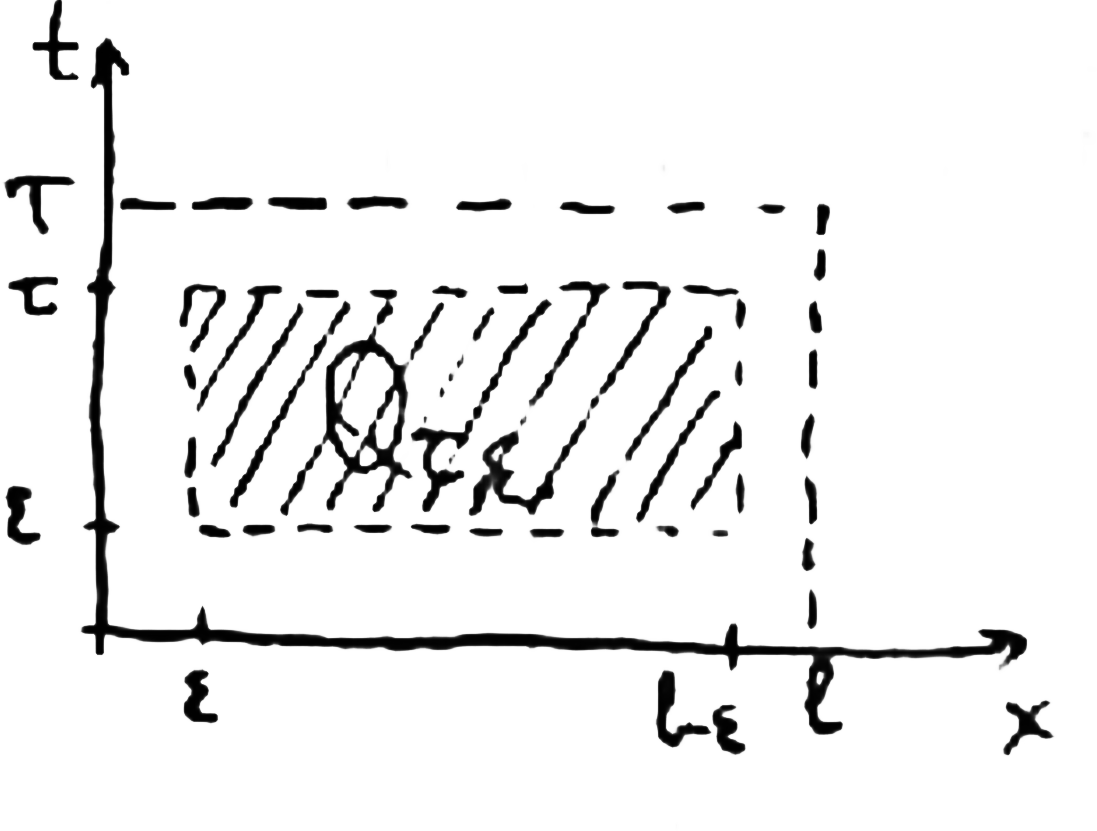
\includegraphics[scale = 0.2]{13_1_new}
\end{center}
\end{minipage}
\begin{minipage}[c]{0.8\textwidth}
$$0 = \iint\limits_{Q_{ \tau, \varepsilon}}I\;dxdt = \iint\limits_{Q_{\tau, \varepsilon}}\div \vec{F}\;dxdt = \oint\limits_{\partial Q_{\tau, \varepsilon}} -\dfrac{V_t^2 + a^2V_{x}^2}{2}\;dx - a^2V_tV_x\;dt$$
\begin{center}
Распишем интеграл по $\partial Q_{\tau, \varepsilon}$:
\end{center}
\end{minipage}
\begin{equation*}
\int\limits_{\varepsilon}^{l - \varepsilon} \biggl( \dfrac{V_t^2 + a^2V_x^2}{2}\biggr)\biggr|_{t = \tau}\;dx - \int\limits_{\varepsilon}^{l - \varepsilon} \biggl( \dfrac{V_t^2 + a^2V_x^2}{2}\biggr)\biggr|_{t = \varepsilon}\;dx - \int\limits_{\varepsilon}^{\tau}\bigl(a^2V_xV_t\bigr)|_{x = l - \varepsilon}\;dt + \int\limits_{\varepsilon}^{\tau}\bigl(a^2V_xV_t\bigr)|_{x = \varepsilon}\;dt = 0
\end{equation*}
В пределе при $\varepsilon \to 0$ получаем :
\begin{align*}
 \because V_t(\varepsilon, x) \to V_t(0, x) = 0\; \; \; \; \; \; \; \because V_x(\varepsilon, x) \to V_x(0, x) = \dfrac{d}{dx}\bigl(V\bigr|_{t = 0} \bigr) = 0 \; \; \; \; \; \; \; \because \int_{\varepsilon}^{l-\varepsilon} \to \int_{0}^{l} {\tiny \text{(по определению несобственного интеграла)}} \\
\because \lim_{\varepsilon \rightarrow +0} V_t(t, l - \varepsilon) = V_t(t, l) = 0 \Rightarrow \cancelto{0}{\int\limits_0^\tau \bigl(a^2V_tV_x\bigr)\;dt}\; \;  \because \int\limits_{\varepsilon}^{l - \varepsilon}
\while{\dfrac{V_t^2 + a^2V_x^2}{2} }{\tau = l}\; dx 
= \cancelto{0}{\int\limits_{0}^l \dfrac{V_t^2(0, x) + a^2V_x^2(0, x)}{2}\;dx\;\;\;\;\;\;}
\end{align*}
Аналогично для $\int\limits_{\varepsilon}^{\tau}(a^2V_tV_x)\bigr|_{x = \varepsilon}\;dt = 0$. Поэтому получаем, что: 
$$\int\limits_{0}^l \dfrac{V_t^2(\tau, x) + a^2V_x^2(\tau, x)}{2}\;dx = 0$$
Тогда $V_t^2(\tau, x) + a^2V_x(\tau, x) = 0 \Forall (x, t) \in (0, l) \times \tau$. \\
В любой точке $(t, x) \in Q_{\tau}\colon\; \vec{\nabla}V(t, x) = \vec{0} \Rightarrow V = \text{const}\Forall(t, x) \in Q_{\tau}$. \\
На замыкании в силу непрерывности $V$ в $\overline{Q}_{\tau}$ также будет $V \equiv \text{const}$, но на границе $V = 0 \Rightarrow V \equiv 0 \Forall (t, x) \in \overline{Q}_{\tau}$, поэтому \textbf{$\tilde{u}_{1} = \tilde{u}_{2}$}.
\paragraph{Существование решения} Будем рассматривать смешанную задачу для однородного уравнения колебаний струны при закреплённых концах.
\begin{equation*}
\label{eq:13_2}
\begin{cases}
	u_{tt} = a^2u_{xx},\; (t, x) \in Q_{\tau}, \\
	u\bigr|_{t = 0} = u_0(x),\; u_t\bigr|_{t = 0} = u_1(x),\; x \in [0, l], \\
	u\bigr|_{x = 0} = u\bigr|_{x = l} = 0,\; t \in [0, \tau].
\end{cases}
\end{equation*}
Рассмотрим дифференциальный оператор $-\Delta_{0}$:
$$\mathcal{D}(-\Delta) =\{X(x) \in C^2[0, l]\colon\; X(0) = X(l) = 0\}$$
У это оператора есть счётное однопараметрическое семейство собственных функий: $\lambda_k = \dfrac{\pi k}{l},\quad X_k = \sin(\lambda_k x),\; k \in \mathbb{N}$. \\
Решение будем искать в виде ряда $u(t, x) = \sum\limits_{k = 1}^{\infty} \Theta_k(t)X_k(x)$. Будем требовать выполнения следующих условий:
\begin{equation}
\begin{cases}
	u_0(x) \in C^3[0, l],\; u_1(x) \in C^2[0, l] - \textbf{условия гладкости}\\
	u_0(0) = u_0(l) = 0 - \text{для непрерывности решения на}\; \overline{Q}_{\tau}, \\
	u_1(0) = u_1(l) = 0 - \text{для принадлежности решения}\; C^1(\overline{Q}_{\tau}), \\
	u^{''}_0(0) = u_0(l)^{''} = 0 - \text{для принадлежности}\; C^2(\overline{Q}_{\tau}).
\end{cases}
\end{equation}

\textit{Последние три условия называются \textbf{условиями согласования}}. \\
Рассматриваемый оператор симметричен относительно скалярного произведения в $\mathbb{L}_2$, значит, собственные функции ортогональны в $\mathbb{L}_2$. Разложим $u_0, u_1$ в ряды Фурье по $X_k$ на $[0, l]$:
\begin{align*}
	u_0(x) = \sum\limits_{k = 1}^{\infty} A_kX_k,\; A_k = \dfrac{2}{l} \int\limits_{0}^l u_0(x)X_k\;dx \\
	u_1(x) = \sum\limits_{k = 1}^{\infty} B_kX_k,\; B_k = \dfrac{2}{l} \int\limits_{0}^l u_1(x)X_k\;dx 
\end{align*}
Формально подставляем в уравнение: $\sum\limits_{k = 1}^{\infty} \Bigl( \ddot{\Theta}_k + a^2 \lambda_k^2\Theta_k \Bigr)X_k = 0$. Из начальных условий: $\Theta_k(0) = A_k,\; \Theta^{\cdotp}_k(0) = B_k$. \\
В силу ортогональности $\{X_k(x)\}_{k = 1}^{\infty}$ получаем счётное число задач Коши:
\begin{equation*}
\begin{cases}
	\Theta^{\cdotp \cdotp}_k + a^2 \lambda_k^2\Theta_k = 0, \\
	\Theta_k(0) = A_k,\; \Theta^{\cdotp}_k(0) = B_k.
\end{cases}
\end{equation*}
Решение: $\Theta_k(t) = A_k\cos \roundBr{\frac{a \pi k}{l}}t + \frac{l}{a \pi k}B_k \sin \roundBr{\frac{a \pi k}{l}}t,\; t \in [0, \tau]$. 
\end{proof}
\subsection{Обоснование метода}
\begin{theorem}
Пусть данные Коши $u_0(x)$ и $u_1(x)$ удовлетворяют условиям гладкости и согласования. Тогда ряд $\sum\limits_{k = 1}^{\infty}\Theta_k(t)X_k(x)$ сходится абсолютно и равномерно в $\overline{Q}_{\tau}$. Его сумма принадлежит классу $C^2(\overline{Q}_{\tau})$ и является классическим решением задачи ~\ref{eq:13_2}. Частные производные по $t$ и $x$ до второго порядка 
включительно можно вычислить почленным дифференцированием ряда.
\end{theorem} 
\begin{proof}
\begin{align*}
	A_k = \dfrac{2}{l}\int\limits_{0}^{l}u_0\sin \roundBr{\dfrac{\pi k}{l}x}\;dx = \cancelto{0}{\dfrac{-2}{l}\dfrac{l}{\pi k}u_0(x)\cos \roundBr{\dfrac{\pi k}{l}x}\biggr|_0^l} + \dfrac{l}{\pi k}\dfrac{2}{l}\int\limits_0^l u_0^{'}\cos \roundBr{\dfrac{\pi k}{l}x}\;dx = \cancelto{0}{\roundBr{\dfrac{l}{\pi k}}^2 \dfrac{2}{l}u_0^{'}(x)\sin \roundBr{\dfrac{\pi k}{l}x}\biggr|_0^l} - \\ - \dfrac{2}{l}\roundBr{\dfrac{l}{\pi k}}^2 \int\limits_0^l u_0^{''}(x)\sin \roundBr{\dfrac{\pi k}{l} x}\;dx = - \roundBr{\dfrac{l}{\pi k}}^3 \underbrace{\dfrac{2}{l} \int\limits_0^l u_0^{'''}(x)\cos \roundBr{\dfrac{\pi k}{l}x}\;dx}_{\alpha_k} + \cancelto{0}{\dfrac{2}{l}\roundBr{\dfrac{l}{\pi k}}^3u_0^{''}(x)\cos \roundBr{\dfrac{\pi k}{l}x}\biggr|_0^l} = - \roundBr{\dfrac{l}{\pi k}}^3 \alpha_k
\end{align*}

\textit{Примечание:} $\alpha_k$ - коэффициенты Фурье функции $u_0^{'''}(x)$ по ортогональной системе функций $\cos \roundBr{\frac{\pi k}{l}}$ --- собственных функций оператора $-\Delta_0$ с граничными условиями Неймана --- тоже симметричного оператора. \\
Аналогично находим коэффициенты $B_k$:
$$B_k = - \roundBr{\dfrac{l}{\pi k}}^2 \beta_k,\; \text{где}\; \beta_k = \dfrac{2}{l} \int\limits_0^l u_1^{''}(x)\sin \roundBr{\dfrac{\pi k}{l} x} \;dx$$
Из того, что
\begin{equation*}
	|u_k(t, x)| = |\Theta_k(t)X_k(k)| = \biggl| A_k \cos (a \lambda_k t) + \dfrac{B_k}{a \lambda_{k}} \sin(a \lambda_{k}) \biggr| \leq \roundBr{\dfrac{l}{\pi k}}^3 |\alpha_k| + \dfrac{1}{a \lambda_k} \roundBr{\dfrac{l}{\pi k}}^2 |\beta_k| \leq \dfrac{c}{k^3}
\end{equation*}
следует абсолютная и равномерная сходимость ряда на $\overline{Q}_{\tau}$
\begin{enumerate}
\item Граничные условия: $u(t, 0) = \sum\limits_{k = 1}^{\infty}(\ldots) \sin(0) = 0, \; \; u(t, l) = \sum\limits_{k = 1}^{\infty}(\ldots)\sin (\pi k) = 0.$ \\
Начальные условия: $u(0, x) = \sum\limits_{k = 1}^{\infty}A_k \sin(\lambda_k x) = u_0(x),\; \; u_t(0, x) = \sum\limits_{k = 1}^{\infty}B_k\sin(\lambda_k x) = u_1(x)$. \\
Итак, ряд порождает непрерывную на $\overline{Q}_{\tau}$ функцию, удовлетворяющую начальным и граничным условиям.
\item Производные: $u_t \displaystyle \sim \sum\limits_{k = 1}^{\infty} \squareBr{-\dfrac{a \pi k}{l}A_k\sin (\lambda_k a t) + B_k\cos (a \lambda_k t)}\sin (\lambda_k x) = \sum\limits_{k = 1}^{\infty} V_k$.
$$|V_k| \leq a \lambda_k |A_k| + |B_k| \leq \dfrac{a \pi k}{l} \roundBr{\dfrac{l}{\pi k}}^3|\alpha_k| + \roundBr{\dfrac{l}{\pi k}}^2 |\beta_k| \leq \dfrac{\tilde{c}}{k^2} \Longrightarrow u_t \in C(\overline{Q}_{\tau})$$   
\end{enumerate}
Значит, $u \in C(\overline{Q}_{\tau})$. \\
$u_{tt} \displaystyle \sim \sum\limits_{k = 1}^\infty \squareBr{-\roundBr{\dfrac{a \pi k}{l}}^2A_k\cos(\lambda_k at) - \dfrac{a \pi k}{l}B_k\sin(\lambda_k at)}\sin(\lambda_k x) = \sum\limits_{k = 1}^{\infty} w_k$.
$$|w_k| = \roundBr{\dfrac{a \pi k}{l}}^2|u_k| \leq \roundBr{\dfrac{a \pi k}{l}}^2\roundBr{\dfrac{l}{\pi k}}^3\roundBr{|\alpha_k| + \dfrac{1}{a}|\beta_k|}$$
Ряд $\sum\limits_{k = 1}^{\infty} w_k$ сходится абсолютно и равномерно, так как: $\sum\limits_{k = 1}^{\infty} |\alpha_k|^2 < \infty, \sum\limits_{k = 1}\dfrac{1}{k^2} < \infty$, а ряд $\sum\limits_{k = 1}^{\infty} \dfrac{\alpha_k}{k}$ сходится абсолютно; поэтому $u(t, x) \in C^2(\overline{Q}_{\tau})$.
\end{proof}
Можно ставить задачу:
\begin{equation*}
	\begin{cases}
	u_{tt} - a^2u_{xx} = f(x), \\
	u\bigr|_{t = 0} = u_0(x), \; u_t\bigr|_{t = 0} = u_1(x), \\
	u\bigr|_{x = 0} = u\bigr|_{x = l} = 0.
	\end{cases}
\end{equation*}
при более широких условиях. \\
При условиях $u_0(x) \in C^2[0, l], \; u_1(x) \in C^1[0, l]$ (гладкости) и $u_0(0) = u_0(l) = u_0^{''}(0) = u_0^{''}(l) = u_1(0) = u_1(l) = 0$ (согласования) и условиях на $f$: $f(t, x), f_x(t, x) \in C(\overline{Q}_{\tau}), f(t, 0) = f(t, l) = 0$ - классическое решение задачи существует и единственно. \\
С помощью метода продолжений делаем $u_0, u_1, f$ нечётными и $2 \pi$ - периодическими, получаем задачу Коши для волнового уравнения. Решение даётся формулой Даламбера.

\end{document}
\newpage
\documentclass[../main.tex]{subfiles}
\begin{document}


\section{Формулы Грина для оператора Лапласа. Постановка краевых задач Дирихле и Неймана для уравнения Пуассона в ограниченной области. Единственность классического решения задачи Дирихле. Неединственность решения задачи Неймана и необходимое условие её разрешимости.}
% Затехал Шлёнский Владос
\Subsection{Формулы Грина}
\begin{definition}
Ограниченная область $\Omega$ называется \textit{областью с гладкой границей}, если $\forall x_0 \in \Gamma = \partial \Omega$ найдутся:
\begin{itemize}
\item такая декартова СК , что начало в $x_0$, $\xi = (\xi_1, \ldots, \xi_n)$ - координаты точек в этой СК
\item Окрестность $U_0(x^0) = \{\xi\colon |\xi^{'}| < r,\; |\xi_n| < h\}$, где $\xi^{'} = (\xi_1, \ldots, \xi_{n - 1})$, такая, что в $U_0(x^0)$ часть границы $\Gamma \bigcap U_0(x^0)$ представляется в виде: $\xi_n = F(\xi^{'}), |\xi^{'}| < r, F(0) = 0,\; F(\xi^{'}) \in C^1(|\xi^{'}| < r),\; \nabla_{\xi^{'}} F(0) = 0$, 
\item Множество $U_{-}(x^0) = U_0(x^0) \bigcap \{x\colon\; \xi_n < F(\xi^{'})\} \in \Omega$, \\
Множество $U_{+}(x^0) = U_0(x^0) \bigcap \{x\colon\; \xi_n \geq F(\xi^{'})\}\colon\; \Omega \bigcap U_{+} = \varnothing$
\item Числа $r > 0$, $h > 0$ можно выбрать независимо от $x^0 \in \Gamma$.
\end{itemize}
\end{definition}
\begin{minipage}{0.3\textwidth}
\begin{center}
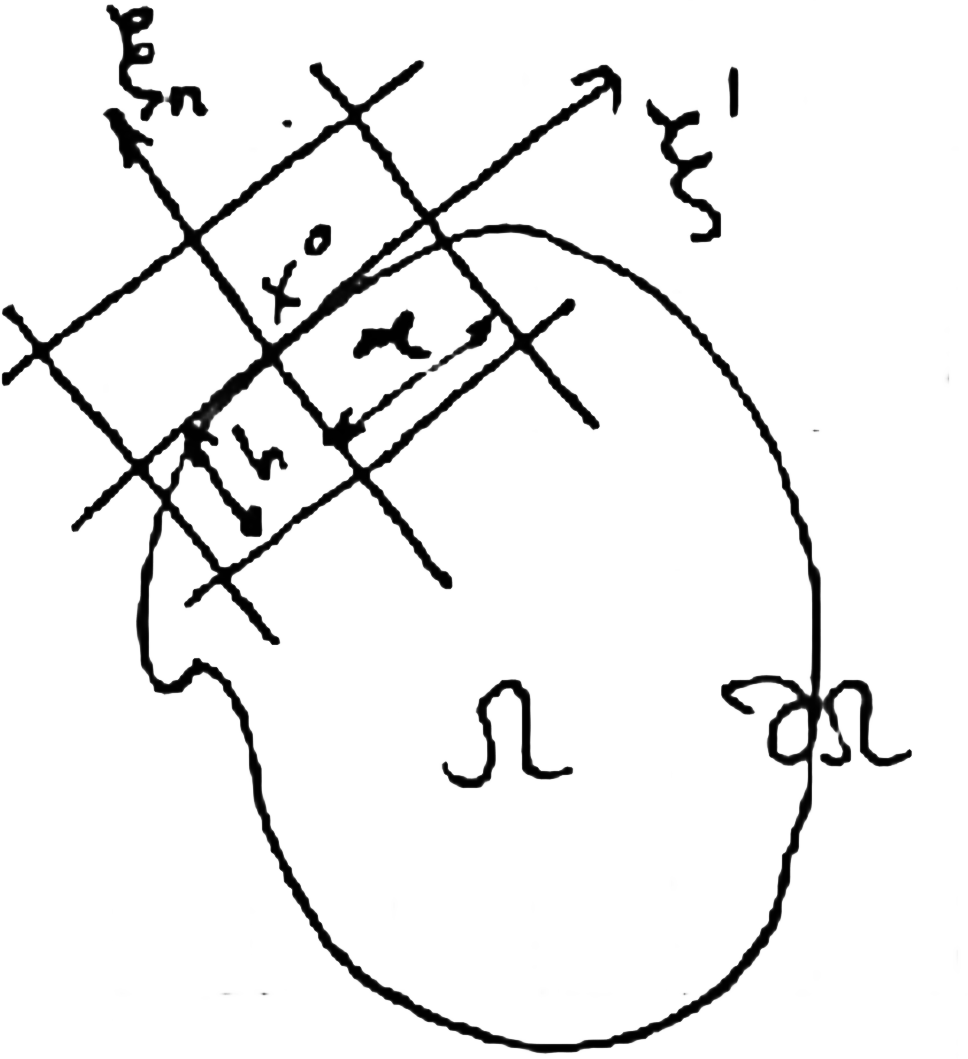
\includegraphics[scale = 0.2]{14_1_new}
\end{center}
\end{minipage}
\begin{minipage}{0.8\textwidth}
Для ограниченных областей с гладкими границами справедлива формула Остроградского-Гаусса ($F$ - непрерывно дифференцируемое векторное поле):
$$\int\limits_{\Omega} \div \vec{F}(x)\;dx = \int\limits_{\partial \Omega} \bigl(\vec{F}(x),\: \vec{n}\bigr)\;dS = \int\limits_{\Gamma} \bigl(\vec{F}(x),\: \vec{n}\bigr)\;dS$$
\end{minipage} \\
\begin{lemma} \ \\
\Subsubsection{Формулы Грина}
Пусть $\Omega$ - ограниченная область с границей класса $C^1$ в $\R^n$, тогда справедливы следующие формулы.
	$$\forall u(x) \in C^2(\Omega)\cap C^1(\overline{\Omega}), v(x) \in C^1(\overline{\Omega}) \to \int\limits_{\Omega} (\Delta u)v\; dx = \oint\limits_{\Gamma} \dfrac{\partial u}{\partial \vec{n}} v\;dS_x - \int\limits_{\Omega}(\nabla u, \nabla v)\;dx $$
$$ \forall u(x) \in C^2(\overline{\Omega}), v(x) \in C^2(\overline{\Omega}) \to \int\limits_{\Omega} (\Delta u)v\; dx - \int\limits_{\Omega} (\Delta v)u\; dx = \oint\limits_{\Gamma} \dfrac{\partial u}{\partial \vec{n}} v\;dS_x - \oint\limits_{\Gamma} \dfrac{\partial v}{\partial \vec{n}} u\;dS_x$$
Полученные формулы называются первой и второй\; \textit{формулами Грина} соответственно.
\end{lemma}
\begin{proof}\ \\
\Subsubsection{Первая формула Грина}
Пусть $\vec{f}(x), v(x)$ - гладкие векторное и скалярное поля соответственно: $\div(\vec{f} \cdot v) = (\nabla, \overset{\shpos}{\vec{f}}v) + (\nabla, \vec{f}\overset{\shpos}{v}) = v\div \vec{f} + (\vec{f}, \grad{v})$. \\
Положим $\vec{f} = \nabla u \in C^1 \Rightarrow \div (v \nabla u) = v \underbrace{\div(\nabla u)}_{\Delta u} + (\nabla u, \nabla v)$. \\
Интегрируем по объёму в $\Omega$:
\begin{equation*}
	\int\limits_{\Omega} v \Delta u\;dx = 	\int\limits_{\Omega} \div(v\nabla u)\;dx -\int\limits_{\Omega} (\nabla u, \nabla v)\;dx = \oint\limits_{\Gamma}(v \nabla u, \vec{n})\;ds - \int\limits_{\Omega}(\nabla u, \nabla v)\;dx
\end{equation*}
Заметим, что:
$$(v\nabla u, \vec{n}) = v \sum\limits_{k = 1}^{\dim \R^n}\dfrac{\partial u(x)}{\partial x_k} n_k = \dfrac{\partial u}{\partial \vec{n}}(x) \cdot v(x)$$
При подстановке данного результата в равенство выше немедленно получим первую формулу Грина.
\Subsubsection{Вторая формула Грина}
Для получения второй формулы Грина необходимо вычесть из первой формулы Грина симметричное ему по $u$ и $v$ равенство:
$$\int\limits_{\Omega} u \Delta v\;dx = \oint\limits_{\Gamma}(u \nabla v, \vec{n})\;ds - \int\limits_{\Omega}(\nabla v, \nabla u)\;dx$$
\end{proof}

\Subsection{Внутрення задача Дирихе для уравнения Пуассона}
Пусть $\Omega$ - ограниченная область с границей $\Gamma$ класса $C^1, u_0(x) \in C(\Gamma), f(x) \in C(\overline{\Omega})$. Требуется найти $u(x)$, удовлетворяющую условиям:
\begin{equation}
\label{eq:14_1}
	\begin{cases}
		\Delta u(x) = f(x), x \in \Omega, \\
		u\bigr|_{\Gamma} = u_0(x).
	\end{cases}
\end{equation}
\textit{Классическим решением задачи Дирихле} ~\ref{eq:14_1} называется $u(x) \in C^1(\overline{\Omega}) \bigcap C^2({\Omega})$, удовлетворяющая уравнению и начальным условиям. \\
\begin{lemma}
Не может существовать более одного классического решения задачи ~\ref{eq:14_1}.
\end{lemma}
\begin{proof}
Если $\exists u_{I}$ и $u_{II}$ - классические решения задачи ~\ref{eq:14_1}, то $v(x) = u_{I} - u_{II}$ есть классическое решение полностью однородной задачи: $\Delta v \equiv 0,\; v\bigr|_{\Gamma} = 0$. \\
По формуле Грина:
\begin{equation*}
	\int\limits_{\Omega} v\cancelto{0}{\Delta v}\; dx = \oint\limits_{\partial \Omega}\dfrac{\partial v}{\partial \vec{n}}\cancelto{0}{v}\;ds - \int\limits_{\Omega}(\nabla v, \nabla v)\;dx \Rightarrow \nabla v \equiv 0 \Forall x \in \Omega \Rightarrow v(x) = \text{const}
\end{equation*}
С учётом того, что $\Delta(x) = 0$ и $v(x)\bigr|_{\Gamma} = 0$, получим, что $v(x) = 0$, а значит, $u_{I} = u_{II}$, и решение единственно.
\end{proof}
\Subsection{Внутренняя задача Неймана для уравнения Пуассона}
Пусть $\Omega$ -ограниченная область с границей класса $C^1, u_1(x) \in C(\Gamma), f(x) \in C(\overline{\Omega})$. Требуется найти $u(x)$ удовлетворяющую условиям:
\begin{equation}
\label{eq:14_2}
	\Delta u(x) = f(x), x \in \Omega, \\
	\dfrac{\partial u}{\partial \vec{n}} = u_1(x), x \in \Gamma.
\end{equation}
\begin{definition}
\textit{Классическое решение задачи Неймана} ~\ref{eq:14_2} есть такая функция $u(x) \in C^1(\overline{\Omega}) \cap C^2({\Omega})$, удовлетворяющая уравнению и граничным условиям.
\end{definition}
\begin{lemma}
Любые два классические решения задачи Неймана отличаются на константу.
\end{lemma}
\begin{proof}
Если $\exists u_{I}$ и $u_{II}$ - классические решения задачи ~\ref{eq:14_2}, то $v(x) = u_{I} - u_{II}$ есть классическое решение полностью однородной задачи: $\Delta v \equiv 0,\; \dfrac{\partial v}{\partial \vec{n}}\bigr|_{\Gamma} = 0$. 
По формуле Грина имеем:
\begin{equation*}
 	\int\limits_{\Omega} \cancelto{0}{\Delta v}v\; dx = \oint\limits_{\Gamma} \cancelto{0}{\dfrac{\partial u}{\partial \vec{n}}}v\;dS - \int\limits_{\Omega} |\nabla v|^2\;dx \Rightarrow v \equiv \text{const}
\end{equation*}
\end{proof}
\begin{lemma}
Необходимым условием существования классического решения задачи Неймана является условие $\int\limits_{\Omega} f(x)\;dx = \oint\limits_{\Gamma}u_1(x)\;dS$
\end{lemma}
\begin{proof}
\begin{equation*}
\int\limits_{\Omega} f(x)\;dx = \int\limits_{\Omega} \Delta u\;dx = \int\limits_{\Omega} \Delta u \cdot 1\; dx = \bigl[\text{1-ая формула Грина}\bigr] = \int\limits_{\partial \Omega} \dfrac{\partial u}{\partial \vec{n}} \cdot 1\;ds - \cancelto{0}{\int\limits_{\Omega} (\nabla u, \nabla 1)\;dx} = \int\limits_{\partial \Omega} u_1(x) \cdot 1\;ds 
\end{equation*}
\end{proof}
\end{document}
\newpage
\section{Решение методом Фурье смешанной задачи для уравнения теплопроводности на отрезке с однородными краевыми условиями Дирихле. Существование и единственность классического решения.}
% Техал Витяй
Рассмотрим смешанную (начально-краевую) задачу:
\begin{equation} \label{15_1}
	\begin{cases}
		u_t - a^2u_{xx} = f(t,x), \quad &0 < t < T, \quad 0 < x < l, \\
		\eval{u}_{t=0} = u_0(x), \quad & 0 \leqslant x \leqslant l, \\
		\eval{u}_{x=0} = \psi_0(t), \quad \eval{u}_{x=l} = \psi_1(t), \quad & 0 \leqslant t \leqslant T.
	\end{cases}
\end{equation}
Рассматриваем ее классическое решение~-- функцию $u(t,x) \in C^{1,2}_{t,x}(Q_T) \cap C(\overline{Q_T})$, где \\ $Q_T = \brk[c]*{(t,x) : t \in (0,T), \, x \in (0,l)}$, удовлетворяющую в $Q_T$ уравнению, начальному и граничным условиям.
\begin{theorem}[Единственности]
	Не может существовать более одного классического решения задачи (\ref{15_1}).
\end{theorem}
\begin{proof}
	Если $u_1, u_2$~-- классические решения, то $v = u_1 - u_2$~-- классическое решение полностью однородной задачи. На параболической границе $\Gamma_T = \brk[c]*{t=0, x \in \brk[s]*{0,l}} \cup \brk[c]*{x=0, t \in \brk[s]*{0,T}} \cup \brk[c]*{x=l, t \in \brk[s]*{0,T}}$ $\eval{v}_{\Gamma_T} = 0$. Но на $\Gamma_T$ достигается максимум и минимум $v$ в $Q_T$ в силу принципа максимума $\Rightarrow v \equiv 0$
\end{proof}

Частный случай, указанный в билете:
\begin{equation*}
	\begin{cases}
		u_t - a^2u_{xx} = 0, \quad & 0 < t < T, \quad 0 < x < l, \\
		\eval{u}_{t=0} = u_0(x), \quad & 0 \leq x \leq l, \\
		\eval{u}_{x=0} = 0, \quad \eval{u}_{x=l} = 0, \quad & 0 \leqslant t \leqslant T.
	\end{cases}
\end{equation*}
Из непрерывности естественно требовать выполнение условий согласования: $u_0(0) = u_0(l) = 0$. Оказывается, в таких условиях решение существует.

{\it Метод Фурье}~-- поиск решения в виде ряда по собственным функциям стационарного оператора.

Придём к этой идее. Будем искать решение $Lu = u_t - a^2u_{xx} = 0$ методом разделения переменных: \\ $u(t,x) = \Theta(t) X(x), \quad u(t,x) \not\equiv 0$.

Подставляем: $\dot{\Theta}(t) X(x) - a^2\Theta(t) X''(x) = 0 \Rightarrow \dfrac{\dot{\Theta}(t)}{a^2\Theta(t)} = \dfrac{X''(x)}{X(x)} = -\lambda = \text{const}$, т.к. равенство выполнено $\forall (t,x) \in Q_T$

Получаем на функции $\Theta$ и $X$ следующие уравнения:
\begin{equation*}
	\begin{cases}
		-X''(x) = \lambda X(x), \quad & 0 \leq x \leq l, \\
		\dot{\Theta}(t) + \lambda a^2 \Theta(t) = 0, \quad & 0 \leq t \leq T.
	\end{cases}
\end{equation*}
Из начального условия $u(t,0) = \Theta(t)X(0) \Forall t \in (0,T) \Rightarrow X(0) = 0$. Аналогично $X(l) = 0$.

Задача для $X$:
\begin{equation}
	\begin{cases}
		-X''(x) = \lambda X(x), \quad x \in (0,l), \\
		X(0) = X(l) = 0, \\
		X(x) \not\equiv 0.
	\end{cases}
\end{equation}
Поставленная задача называется {\it задачей Штурма-Лиувилля}.

Введем оператор $A$:
\begin{itemize}
	\item $\mathrm{D}(A) = \brk[c]*{X \in C^2[0,l] : X(0) = X(l) = 0}$
	\item $\mathrm{Im}(A) = \brk[c]*{Y \in C[0,l]}$
	\item $AX = -\Delta X = Y$
\end{itemize}

Задача Штурма-Лиувилля~-- это задача на собственные функции и собственные значения оператора $A$.

Решим ее:
\begin{itemize}
	\item $\lambda < 0$:

		$X(x) = C_1e^{\sqrt{\abs*{\lambda}}x} + C_2e^{-\sqrt{\abs*{\lambda}}x}$

			$\begin{cases}
				X(0) = C_1 + C_2 = 0, \\
				X(l) = C_1e^{\sqrt{\abs*{\lambda}}l} + C_2e^{-\sqrt{\abs*{\lambda}}l} = 0.
			\end{cases}$

			$\text{det}\begin{pmatrix} 1 & 1 \\ e^{2\sqrt{\abs*{\lambda}}l} & 1 \end{pmatrix} = 1 - e^{2\sqrt{\abs*{\lambda}}l} = 0 \Rightarrow \sqrt{\abs*{\lambda}}l = 0$, противоречие.

			Итак, <<$-\Delta$>> с граничными условиями Дирихле не имеет отрицательных собственных значений.

	\item $\lambda = 0$:

		$X(x) = C_1x + C_2$

		$\begin{cases}
			X(0) = C_2 = 0, \\
			X(l) = C_1l = 0.
		\end{cases}$

		Нетривиальных решений нет.

	\item $\lambda > 0$:

		$X(x) = C_1\cos\sqrt{\lambda}x + C_2\sin\sqrt{\lambda}x$

		$\begin{cases}
			X(0) = C_1 = 0, \\
			X(l) = C_2\sin\sqrt{\lambda}l = 0.
		\end{cases}$

		$\sqrt{\lambda}l = \pi k \Rightarrow \lambda_k = \brk*{\dfrac{\pi k}{l}}^2, k \in \N$

		Функции $X_k(x) = \sin\brk*{\dfrac{\pi k}{l}x}$
\end{itemize}
Теперь для найденных $\lambda_k$ решаем $\dot{\Theta}_k(t) + \lambda_k a^2 \Theta_k(t) = 0 \Rightarrow \Theta_k(t) = e^{-a^2\lambda_kt}$

Мы нашли $u_k(t,x) = e^{-a^2\lambda_kt}\sin\brk*{\dfrac{\pi k}{l}}$~-- счетное число бесконечно гладких решений: $u_k$ удовлетворяет задаче

\begin{equation*}
	\begin{cases}
		\brk*{u_k}_t - a^2\brk*{u_k}_{xx} = 0, \\
		u_k(t,0) = u_k(t,l) = 0, \\
		u_k(0,x) = X_k(x) = \sin\lambda_kx.
	\end{cases}
\end{equation*}
Тогда $u_A(t,x) = \displaystyle\sum\limits_{k=1}^N A_k u_k(t,x)$~-- решение для задачи с начальным условием $u(0,x) = \displaystyle\sum\limits_{k=1}^N A_k X_k(x)$.

Обозначим $Ku_0$~-- класс функций $u_0 = \displaystyle\sum\limits_{k=1}^N A_k X_k(x)$~-- тех, для которых умеем выписать явное решение. Пусть $A_k$~-- $k$-мерные векторы. Между $Ku_0$ и $A_k$ есть биекция (по $u_0 = \displaystyle\sum\limits_{k=1}^N A_k X_k(x)$ однозначно восстанавливаем $A_k = \dfrac{2}{l}\displaystyle\int\limits_0^l u_0(x) \sin\brk*{\dfrac{\pi k}{l}x}dx$)

Бесконечномерный вектор подойдет уже не всегда. Как минимум ряд $\displaystyle\sum\limits_{k=1}^\infty A_k X_k(x)$ должен сойтись в замыкании области. Функция $\displaystyle\sum\limits_{k=1}^\infty A_k u_k(t,x)$ должна быть нужной гладкости, а также удовлетворять уравнению (\ref{15_1}).

\begin{statement}
	$\brk[c]*{A_k}_{k=1}^{\infty}: \displaystyle\sum\limits_{k=1}^{\infty} \abs*{A_k} < \infty$ подойдет.
\end{statement}

\begin{proof}
	Пусть $u_0(x) = \displaystyle\sum\limits_{k=1}^{\infty} A_k\sin\brk*{\dfrac{\pi k}{l}x}, \displaystyle\sum\limits_{k=1}^{\infty} \abs*{A_k} < \infty$. Тогда $\abs*{A_k\sin\brk*{\dfrac{\pi k}{l}x}} \leqslant \abs*{A_k} \Rightarrow$ по теореме Вейерштрасса ряд сходится абсолютно и равномерно $\Rightarrow$ сумма непрерывна.

	Равномерно сходящийся ряд можно почленно интегрировать $\Rightarrow$ по $u_0(x)$ восстанавливаем $A_n$: $\displaystyle\int\limits_0^l u_0(x)\sin\brk*{\dfrac{\pi n}{l}x}dx = \displaystyle\sum_{k=1}^{\infty} A_k \displaystyle\int\limits_0^l \sin\brk*{\dfrac{\pi k}{l}x} \sin\brk*{\dfrac{\pi n}{l}x} dx \Rightarrow A_n = \dfrac{2}{l} \displaystyle\int\limits_0^l u_0(x) \sin\brk*{\dfrac{\pi n}{l}x} dx$

	Теперь рассмотрим ряд $u_A(t,x) \sim \displaystyle\sum\limits_{k=1}^{\infty} A_k e^{-\brk*{\frac{a\pi k}{l}}^2t} \sin\brk*{\dfrac{\pi k}{l}x}$

	Пока не можем поставить знак равенства, поскольку еще не выяснили сходимость.

	$\abs*{A_k e^{-\brk*{\frac{a\pi k}{l}}^2t} \sin\brk*{\dfrac{\pi k}{l}x}} \leqslant \abs*{A_k} \Rightarrow$ ряд сходится абсолютно и равномерно, и мы можем поставить знак равенства:

	$u_A(t,x) = \displaystyle\sum\limits_{k=1}^{\infty} A_k e^{-\brk*{\frac{a\pi k}{l}}^2t} \sin\brk*{\dfrac{\pi k}{l}x}$

	Покажем, что получилась $u_A(t,x) \in C^\infty(t>0, \, 0 \leqslant x \leqslant l)$. 

	Возьмем прямоугольник $Q_\delta = \brk[c]*{(t,x) : t \geqslant \delta > 0, \, 0 \leqslant x \leqslant l}$. 

	Формально $\dfrac{\partial u_A}{\partial t} \sim -\displaystyle\sum\limits_{k=1}^{\infty} A_k\brk*{\dfrac{a\pi k}{l}}^2 e^{-\brk*{\frac{a\pi k}{l}}^2t} \sin\brk*{\dfrac{\pi k}{l}x} = -\displaystyle\sum\limits_{k=1}^{\infty} \varphi_k(t,x)$

	Для краткости введём $y = \brk*{\dfrac{a\pi k}{l}}^2$.

	Оценка: $\abs*{\varphi_k} \leqslant \abs*{A_k}ye^{-y\delta} = \abs*{A_k} \dfrac{1}{\delta} (y\delta) e^{-y\delta} \leqslant \abs*{A_k} \dfrac{1}{\delta e}$

	Последнее неравенство следует из того, что функция $xe^{-x}$ имеет максимум в точке $x = 1$, равный $\dfrac{1}{e}$.

	Итак, по теореме Вейерштрасса, ряд сходится абсолютно и равномерно.

	Варьируя $\delta$, прямоугольниками $Q_\delta$ заметаем всю область $\brk[c]*{t > 0, 0 \leqslant x \leqslant l}$

	Для остальных производных получим то же самое~-- всегда будет получаться произведение многочлена на экспоненту с отрицательным показателем.

	Мы научились решать задачу для $u_0(x) = \displaystyle\sum\limits_{k=1}^{\infty} A_k \sin\brk*{\dfrac{\pi k}{l}x}$.
\end{proof}

Докажем серию лемм.
\begin{lemma}
	Пусть в гильбертовом пространстве $\mathcal{H}$ оператор $A$ симметричный (самосопряжённый), т.е. $(Ax,y) = (x,Ay)$. Тогда:
	\begin{enumerate}
		\item Все собственные значения $A$ вещественны;
		\item Собственные функции, отвечающие различным собственным значениям, ортогональны.
	\end{enumerate}
\end{lemma}
\begin{proof}
	Пусть $x_k$~-- собственный вектор, отвечающий собственному значению $\lambda_k$, а $x_n$~-- собственный вектор, отвечающий собственному значению $\lambda_n$, причем $\lambda_k \not= \lambda_n$. Тогда:
	\begin{enumerate}
		\item $\lambda_k(x_k, x_k) = (Ax_k, x_k) = (x_k, Ax_k) = (x_k, \lambda_kx_k) = \overline{\lambda_k}(x_k, x_k) \Rightarrow \lambda_k = \overline{\lambda_k} \Rightarrow \mathrm{Im} \, \lambda_k = 0$
		\item $\lambda_k(x_k, x_n) = (Ax_k, x_n) = (x_k, Ax_n) = \overline{\lambda_n}(x_k,x_n) \underset{\text{пункт 1}}{=} \lambda_n(x_k,x_n) \Rightarrow \underset{\not= 0}{\underline{(\lambda_k - \lambda_n)}}(x_k,x_n) = 0 \Rightarrow (x_k,x_n) = 0$
	\end{enumerate}
\end{proof}
\begin{lemma}
	Оператор $A = -\dfrac{d^2}{dx^2}$, определенный на $\mathrm{D}(A)$, является симметричным относительно скалярного произведения в $L_2[0,l]: (u,v) = \displaystyle\int\limits_0^l u(x) \overline{v(x)} dx$.
\end{lemma}
\begin{proof}
	$(Au,v) = \displaystyle\int\limits_0^l (-u''(x))\overline{v(x)}dx = \underset{= 0, \text{ в силу определения $\mathrm{D}(A)$}}{\underline{\left.-u'(x)\overline{v(x)}\right|_0^l}} + \displaystyle\int\limits_0^l u'(x) \overline{v'(x)} dx = \underset{= 0, \text{ в силу определения $\mathrm{D}(A)$}}{\underline{\left.u(x)\overline{v'(x)}\right|_0^l}} + \displaystyle\int\limits_0^l u(x)\brk*{-\overline{v''(x)}}dx = (u, Av)$
\end{proof}
\begin{lemma}
	Пусть $\brk[c]*{e_k}$~-- не более чем счетная ортогональная система в линейном пространстве со скалярным произведением: $(e_k, e_j) = \delta_{kj} \underset{>0}{\underline{(e_k, e_k)}}$. Тогда $\forall f$ из этого пространства справедливо неравенство Бесселя: $\displaystyle\sum\limits_{k=1}^{\infty} \abs*{c_k}^2 (e_k, e_k) = \displaystyle\sum\limits_{k=1}^{\infty} \abs*{\dfrac{(f,e_k)}{(e_k,e_k)}}^2 (e_k, e_k) \leq (f, f)$.
\end{lemma}
\begin{proof}
	$0 \leq \brk*{f - \displaystyle\sum\limits_{k=1}^n c_ke_k, f - \displaystyle\sum\limits_{k=1}^n c_ke_k} = (f,f) - \displaystyle\sum\limits_{k=1}^n c_k(e_k,f) - \displaystyle\sum\limits_{j=1}^n \overline{c_j} (f,e_j) + \\ + \displaystyle\sum\limits_{k=1}^n \displaystyle\sum\limits_{j=1}^n c_k \overline{c_j} (e_k, e_j) = (f,f) - \displaystyle\sum\limits_{k=1}^n c_k \overline{c_k} (e_k, e_k) - \displaystyle\sum\limits_{j=1}^n c_j \overline{c_j} (e_j, e_j) + \displaystyle\sum\limits_{i=1}^n c_i \overline{c_i} (e_i, e_i) = \\ = (f,f) - \displaystyle\sum\limits_{k=1}^n \abs*{c_k}^2 (e_k, e_k)$. 
    
    Переходя к пределу при $n \to \infty$, получаем $\displaystyle\sum\limits_{k=1}^{\infty} \abs*{c_k}^2 (e_k, e_k) \leq (f,f)$.
\end{proof}
\begin{lemma}
	Пусть два ряда $\displaystyle\sum\limits_{k=1}^{\infty} \abs*{\alpha_k}^2 = A, \: \displaystyle\sum\limits_{k=1}^{\infty} \abs*{\beta_k}^2 = B$ сходятся. Тогда ряд $\displaystyle\sum\limits_{k=1}^{\infty} \alpha_k \beta_k$ сходится абсолютно, причем $\displaystyle\sum\limits_{k=1}^{\infty} \abs*{\alpha_k \beta_k} \leq \sqrt{A} \sqrt{B}$.
\end{lemma}
\begin{proof}
	$\displaystyle\sum\limits_{k=1}^{n} \abs*{\alpha_k \beta_k} \underset{\text{КБШ}}{\leq} \sqrt{\displaystyle\sum\limits_{k=1}^{n} \abs*{\alpha_k}^2} \sqrt{\displaystyle\sum\limits_{k=1}^{n} \abs*{\beta_k}^2}$. Переходя к пределу при $n \to \infty$, получаем требуемое.
\end{proof}
\begin{lemma}
	Пусть $v(x) \in C^1[0,l], \, v(0) = v(l) = 0$. 

	Тогда ряд $\displaystyle\sum\limits_{k=1}^{\infty} A_k \sin\brk*{\dfrac{\pi k}{l}x}$, где $A_k = \dfrac{2}{l}\displaystyle\int\limits_0^l v(y)\sin\brk*{\dfrac{\pi k}{l}y}dy$, сходится на $[0,l]$ к $v(x)$ абсолютно и равномерно.
\end{lemma}
\begin{proof}
	\begin{enumerate}
		\item Система $\brk[c]*{e_k} = \brk[c]*{\sin\brk*{\dfrac{\pi k}{l}x}}$ ортогональна относительно скалярного произведения в $L_2 [0,l]$, так как состоит из собственных функций оператора <<$-\Delta$>> с однородными условиями Дирихле~-- симметричного в $L_2 [0,l]$ оператора.
		\item $A_k = \dfrac{(v,e_k)}{(e_k,e_k)},$ ряд $\displaystyle\sum\limits_{k=1}^{\infty} \abs*{A_k}^2 < \infty$ по неравенству Бесселя.
		\item $A_k = \underset{=0}{\underline{-\left.\dfrac{2}{l} \dfrac{l}{\pi k} v(y) \cos\brk*{\dfrac{\pi k}{l}y}\right|_0^l}} + \dfrac{2}{l} \dfrac{l}{\pi k} \displaystyle\int\limits_0^l v'(y) \cos\brk*{\dfrac{\pi k}{l}y}dy = \dfrac{l}{\pi k} \alpha_k$, где $\alpha_k = \dfrac{2}{l} \displaystyle\int\limits_0^l v'(y) \cos\brk*{\dfrac{\pi k}{l}y}dy$.
		\item Ряд $\displaystyle\sum\limits_{k=1}^{\infty} \abs*{\alpha_k}^2 < \infty$ по неравенству Бесселя, т.к. система $\brk[c]*{g_k} = \brk[c]*{\cos\brk*{\dfrac{\pi k}{l}x}}$ ортогональна относительно скалярного произведения в $L_2 [0,l]$, так как состоит из собственных функций оператора <<$-\Delta$>> с однородными условиями Неймана~-- симметричного в $L_2 [0,l]$ оператора.

		Ряд $\displaystyle\sum\limits_{k=1}^{\infty} \dfrac{1}{k^2} = \dfrac{\pi^2}{6}$ сходится. Тогда сходится абсолютно ряд $\displaystyle\sum\limits_{k=1}^{\infty} \dfrac{\alpha_k}{k} \Rightarrow \displaystyle\sum\limits_{k=1}^{\infty} \abs*{A_k} < \infty$. 

		Функция $\varphi(x) = \displaystyle\sum\limits_{k=1}^{n} A_k \sin\brk*{\dfrac{\pi k x}{l}}$ непрерывна.
		\item Сходимость к $v(x)$: Построим
			\begin{equation*}
				\tilde{v}(x) = \begin{cases} v(x), & x \in [0,l] \\ -v(-x), & x \in [-l,0] \end{cases}
			\end{equation*}
			Затем продолжим на $\R$, сделав периодической: $\tilde{v}(x+2l) = \tilde{v}(x)$.
			Получаем непрерывную периодическую функцию, а во всех точках $x \in [0,l] \Exists \tilde{v}'_-(x), \tilde{v}'_+(x)$. Тогда ряд Фурье этой функции сходится к ней на всей $\R$. В силу нечетности $\tilde{v}$, этот ряд~-- только по синусам, а коэффициенты Фурье равны $A_k$ (для них совпадают формулы). Значит, на $[0,l]$ имеем $v(x) = \displaystyle\sum\limits_{k=1}^{\infty} A_k \sin\brk*{\dfrac{\pi k}{l}x}$
	\end{enumerate}
\end{proof}
Таким образом, доказана теорема:
\begin{theorem}
	Пусть в смешанной задаче
	\begin{equation*}
		\begin{cases}
			u_t - a^2u_{xx} = 0, \quad & 0 < t < T, \quad 0 < x < l, \\
			\eval{u}_{t=0} = u_0(x), \quad & 0 \leq x \leq l, \\
			\eval{u}_{x=0} = \eval{u}_{x=l} = 0, \quad & 0 \leq t \leq T.
		\end{cases}
	\end{equation*}
	функция $u_0(x)$ удовлетворяет условиям гладкости $\brk*{u_0 \in C^1[0,l]}$ и согласования $\brk*{u_0(0) = u_0(l) = 0}$. Тогда ряд $\displaystyle\sum\limits_{k=1}^{\infty} A_k e^{-\brk*{\frac{a\pi k}{l}}^2t} \sin\brk*{\dfrac{\pi k}{l}x} = u(t,x)$, где $A_k = \dfrac{2}{l} \displaystyle\int\limits_0^l u_0(x) \sin\brk*{\dfrac{\pi k}{l}x} dx$, сходится абсолютно и равномерно в $\overline{Q_T} = [0,T] \times [0,l]$, функция $u(t,x) \in C(\overline{Q_T}) \cap C^{\infty}(Q_T)$ и является классическим решением этой задачи, а любая производная при $t > 0$ от $u(t,x)$ может быть найдена почленным дифференцированием.
\end{theorem}

\newpage
% Затехал Хасянов Расул
\section{Решение методом Фурье задачи Дирихле для уравнения Лапласа в круге. Представление решения в виде ряда по однородным гармоническим многочленам и в виде интеграла Пуассона. Существование классического решения при непрерывной граничной функции.} 
\Subsection{Решение методом Фурье задачи Дирихле для уравнения Лапласа в круге.}
Задача: в круге $D = \brk[c]*{x| \abs*{x} < R}$ и на границе $\Gamma =\partial D$ рассматриваем задачу:
\begin{equation} \label{16_1}
\begin{cases}
&\Delta u(x) = f(x), x \in D \longleftarrow \text{уравнение Пуассона}\\
&\eval{u}_\Gamma = u_0(x), x \in \partial D
\end{cases}
\end{equation}
Сделаем замену: 
$x_1 = \rho \cos \varphi, x_2 = \rho \sin \varphi$.\\ Функция $\hat u(\rho,\varphi) = u(\rho \cos \varphi, \rho \sin \varphi)$. \\Аналогично $\hat u_0(\rho, \varphi) = u_0(\rho \cos \varphi, \rho \sin \varphi), \hat f(\rho, \varphi) = f(\rho \cos \varphi, \rho \sin \varphi).$\\
Задача перепишется в виде: 
\[
\begin{cases}
&\hat u_{\rho \rho} + \frac{1}{\rho} \hat u_\rho + \frac{1}{\rho^2} \hat u_{\varphi \varphi} = \hat f(\rho, \varphi), 0 < \rho < R, 0 \leq \varphi \leq 2\pi\\
&\hat u (R,\varphi) = \hat u_0(R, \varphi)\\
&\hat u(\rho,\varphi) = \hat u(\rho, \varphi + 2\pi)
\end{cases}
\]
Далее считаем $\hat f = 0$, то есть решаем уравнение Лапласа.\\
Предположение: $u_0(x) \in C^1(\Gamma)$. Предполагаем, что решение принадлежит классу $C^2(D) \cap C^1(\bar D)$. При этом $\hat u$ -- $2\pi$-периодическая по $\varphi \Rightarrow$ можно разложить $\hat u_0, \hat u$ в ряды Фурье. [Если был было уравнение Пуассона -- требовали бы  $f \in C^1(\bar D)$.]
\begin{align*}
\brk[c]*{\begin{matrix} \hat u(\rho,\varphi) \\ \hat u_0(R,\varphi) \end{matrix}} &= \frac{1}{2} \brk[c]*{\begin{matrix} a_0(\rho) \\ A_0 \end{matrix}} + \sum_{k=1}^{\infty} \brk[s]*{\brk[c]*{\begin{matrix} a_k(\rho) \\ A_k \end{matrix}} \cos k \varphi + \brk[c]*{\begin{matrix} b_k(\rho) \\ B_k \end{matrix}} \sin k \varphi}, \text{где}\\
\brk[c]*{\begin{matrix} a_k(\rho)\\ A_k \end{matrix}} &= \frac{1}{\pi} \int_0^{2\pi} \brk[c]*{\begin{matrix} \hat u(\rho,\psi) \\ \hat u_0(R,\psi) \end{matrix}} \cos k \psi d \psi, k \in \N_0,\\ 
\brk[c]*{\begin{matrix} b_k(\rho)\\ B_k \end{matrix}} &= \frac{1}{\pi} \int_0^{2\pi} \brk[c]*{\begin{matrix} \hat u(\rho,\psi) \\ \hat u_0(R,\psi) \end{matrix}} \sin k \psi d \psi, k \in \N.
\end{align*}
Формально подставляем в уравнение(аргументы функций опускаем -- они все уже определены).
\[
\frac{1}{2}\brk*{a''+\frac{1}{\rho}a_0'} + \sum_{k=1}^\infty \brk[c]*{\brk[s]*{a_k''+\frac{1}{\rho}a_k'-\frac{k^2}{\rho^2}a_k} \cos k \varphi + \brk[s]*{b_k''+\frac{1}{\rho}b_k'-\frac{k^2}{\rho^2}b_k} \sin k \varphi} = 0
\]
Из граничного условия: 
\[
\frac{1}{2}a_0(R) + \sum_k \brk[s]*{a_k(R) \cos k \varphi + b_k(R) \sin k \varphi} = \frac{1}{2} A_0 + \sum_k \brk[s]*{A_k \cos k \varphi + B_k \sin k \varphi}
\]
В силу ортогональности тригонометрической системы в $L_2[0,2\pi]$ имеем на $a_k$ и $b_k$ следующие задачи:
\[
\begin{cases}
&a_k''(\rho)+ \frac{1}{\rho} a_k'(\rho) - \frac{k^2}{\rho^2} a_k(\rho) = 0, 0 \leq \rho \leq R\\
&a_k(R) = A_k, \ k \in \N_0\\
\end{cases} \qquad \begin{cases}
&b_k''(\rho)+ \frac{1}{\rho} b_k'(\rho) - \frac{k^2}{\rho^2} b_k(\rho) = 0, 0 \leq \rho \leq R\\
&b_k(R) = B_k, \ k \in \N\\
\end{cases}
\]
Будем искать только ограниченные решения -- для этого одного граничного условия окажется достаточно.\\
Решения данных уравнений Эйлера ищем в виде $\alpha \rho^\mu$:\\
Для первой серии задачи: $\alpha[\mu(\mu-1)+\mu - k^2] \rho^{\mu-2} = 0 \Rightarrow \mu = \pm k$.\\
Общее решение:
$$ a_k(\rho) = C_{1k}\rho^k+C_{2k}\rho^{-k} $$
$$a_0(\rho) = C_{10} \cdot 1 + C_{20} \cdot \ln \rho$$
Для ограниченности в круге берем $C_{2k} = C_{20} = 0 \Rightarrow a_k = C_{1k} \rho^k, C_{1k} = \frac{A_k}{R^k}, k \in \N_0$.\\
Итак, 
\begin{equation}\label{16_2}
\brk[c]*{\begin{matrix} a_k(\rho)\\ b_k(\rho) \end{matrix}} = \brk[c]*{\begin{matrix} A_k\\ B_k \end{matrix}}\brk*{\frac{\rho}{R}}^k \Rightarrow \hat u(\rho, \varphi) = \frac{A_0}{2} + \sum_{k=1}^{\infty}\brk*{A_k \cos k \varphi + B_k \sin k \varphi} \brk*{\frac{\rho}{R}}^k  
\end{equation}
Вернемся в исходные переменные. Заметим, что если ввести $z = x_1+ix_2 = \rho e^{i \varphi}$, то $\rho^k \cos k \varphi = \mathrm{Re} \ z^k,\\ \rho^k \sin k \varphi = \mathrm{Im} \ z^k$.\\ Обозначим $\mathrm{Re} \ z^k = p_k(x_1,x_2), \mathrm{Im} \ z^k = q_k(x_1,x_2)$.
\begin{equation} \label{16_3}
\Rightarrow u(x_1,x_2) = \frac{A_0}{2}+ \sum_{k=1}^{\infty}\brk[s]*{\frac{A_k}{R^k} p_k(x_1,x_2) + \frac{B_k}{R^k} q_k(x_1,x_2)} 
\end{equation}
\Subsection{Представление решения в виде ряда по однородным гармоническим многочленам и в виде интеграла Пуассона. Существование классического решения при непрерывной граничной функции.}
\begin{theorem}
Пусть $u_0 \in C(\Gamma)$. Тогда:
\begin{enumerate}
\item Существует и единственно классическое решение $u(x) \in C^\infty(D) \cap C(\bar D)$ задачи \ref{16_1} с $f \equiv 0$.
\item В $D$ это решение представимо рядами \ref{16_2} и \ref{16_3}, сходящимися в $|x| \leq R_1 < R$ равномерно.
\item Классическое решение представимо формулой Пуассона: \[u(x) = \frac{1}{2\pi R} \oint_{\partial D} \frac{R^2 - |x|^2}{|x- \xi|^2}u_0(\xi) dS_\xi\]
\item Любые частные производные по $x_1$ и $x_2$ вычисляются почленным дифференцированием ряда.
\end{enumerate}
\end{theorem}
\begin{proof}
\begin{enumerate}
\item Единственность докажем позднее (в этом билете ее нет).
\item Пусть $|u_0| < M$ на $\Gamma$. Тогда: 
\[
\abs*{A_k} \leq \frac{1}{\pi}\int_0^{2\pi} \abs*{u_0} \abs*{\cos k \psi} d \psi \leq 2M, \; \abs*{B_k} \leq 2M
\]
Запишем 
\[u(x_1,x_2) = \frac{A_0}{2}+ \sum_{k=1}^{\infty}\brk[s]*{\frac{A_k}{R^k} p_k(x_1,x_2) + \frac{B_k}{R^k} q_k(x_1,x_2)}  = \mathrm{Re}\, w_1 + \mathrm{Im}\, w_2, \text{где}\]
\[
w_1 = \frac{A_0}{2}+ \sum_{k=1}^{\infty} \frac{A_k}{R_k}z^k,\; w_2 = \sum_{k=1}^{\infty} \frac{B_k}{R_k}z^k
\]
Оба ряда сходятся абсолютно и равномерно в круге $|z| \leq R_1 < R \Rightarrow$ порождают в круге радиуса $R_1$ регулярные функции, что и требовалось.
\item Докажем формулу Пуассона: 
\begin{align*}
\hat u(\rho, \varphi) &= \frac{1}{2}\cdot \frac{1}{\pi} \int_0^{2\pi} \hat u_0(R,\psi) d \psi + \sum_{k=1}^{\infty} \frac{1}{\pi} \int_0^{2\pi} \hat u_0(\psi)\brk*{\cos k \psi \cdot \cos k \varphi + \sin k \psi \sin k \varphi}d\psi \brk*{\frac{\rho}{R}}^k =  \\
&= \brk*{\text{сходимость равномерная}} = \frac{1}{2\pi}\int_0^{2\pi} \brk[s]*{1+ \sum_{k=1}^\infty 2\cos k(\psi - \varphi) \brk*{\frac{\rho}{R}}^k}\hat u_0(\psi) d \psi = \\
& = \frac{1}{2\pi}\int_0^{2\pi} \brk[s]*{\sum_{k=0}^{\infty} e^{-ik(\psi-\varphi)}\brk*{\frac{\rho}{R}}^k + \sum_{k=1}^{\infty} e^{ik(\psi-\varphi)}\brk*{\frac{\rho}{R}}^k} \hat u_0(\psi) d \psi = \frac{1}{2\pi}\int_0^{2\pi} \brk[s]*{\sum_{k=0}^{\infty} p^k + \sum_{k=1}^{\infty} \bar p^k} \hat u_0(\psi) d \psi 
\end{align*}
Под интегралом ($|p| = |\bar p| = \frac{\rho}{R} < 1$): 
\begin{align*}
\sum_{k=1}^{\infty} p^k + \sum_{k=1}^{\infty} \bar p^k &= \frac{1}{1-p} + \frac{1}{1-\bar p} - 1 = \frac{1 - p + 1 - \bar p -1 +p + \bar p - p \bar p}{(1-p)(1-\bar p)} = \frac{1- \abs*{p}^2}{1-(p+\bar p) + p\bar p} = \\
&=\frac{1- \abs*{p}^2}{1-2 \mathrm{Re}\, p + \abs*{p}^2} = \frac{1- \brk*{\frac{\rho}{R}}^2}{1-2\frac{\rho}{R} \cos(\psi - \varphi) + \frac{\rho^2}{R^2}} = \frac{R^2 -\rho^2}{R^2 + \rho^2 -2R\rho\cos(\varphi - \psi)} = \\
&=\frac{R^2 - \abs*{x}^2}{\abs*{x-\xi}^2},\; \begin{matrix} x = (\rho, \varphi)\\ \xi = (R, \psi) \end{matrix}
\end{align*}
Итак, 
\begin{align*}
\hat{u}(\rho, \varphi) &= \frac{1}{2\pi R} \int_0^{2\pi} \frac{R^2 -\rho^2}{R^2 + \rho^2 -2R\rho\cos(\varphi - \psi)} \hat u_0(\psi) d \psi\\
\Longleftrightarrow u(x) &= \frac{1}{2\pi R}\oint_{\Gamma} \frac{R^2 - |x|^2}{|x - \xi|^2}u_0(\xi) dS_\xi
\end{align*}
Заметим, что при $u_0 \equiv 1$ мы получим ядро Пуассона:
\[
1 \equiv \frac{1}{2\pi R}\oint_{\Gamma} \frac{R^2 - |x|^2}{|x - \xi|^2} dS_\xi
\]
Покажем, что $u(x) \in C (\bar D)$.\\
Пусть $x \in D \cap \brk[c]*{x : \abs*{x-x^0} < \delta_{n_0}}$, где $x_0 \in \Gamma$, а $\delta_{n_0}$ выбрано так, чтобы $\abs*{u_0(x) - u_0(x^0)} \leq \varepsilon$.
\begin{align*}
u(x) - u(x^0) &= \frac{1}{2\pi R}\oint_{\Gamma} \frac{R^2 - |x|^2}{|x - \xi|^2}\brk*{u_0(\xi)-u_0(x^0)} dS_\xi = \\
&= \frac{1}{2\pi R} \brk*{\int_{\brk[c]*{\xi \in \Gamma: \abs*{\xi - x^0} < \delta_{n_0}}} +  \int_{\brk[c]*{\xi \in \Gamma: \abs*{\xi - x^0} \geq \delta_{n_0}}}} \frac{R^2 - |x|^2}{|x - \xi|^2}\brk*{u_0(\xi)-u_0(x^0)} dS_\xi = I_< + I_\geq
\end{align*}
\begin{align*}
\abs*{I_<} \leq & \frac{1}{2 \pi R} \int_{(<)}  \frac{\abs*{R^2 - |x|^2}}{|x - \xi|^2}\abs*{u_0(\xi)-u_0(x^0)} dS_\xi \leq \varepsilon \cdot \brk[c]*{\text{ядро Пуассона}} = \varepsilon\\
\abs*{I_\geq} \leq & \frac{1}{2\pi R}\frac{(R - \abs*{x})(R+\abs*{x})}{\min \abs*{\xi - x}^2} \cdot 2M \cdot \int_{(\geq)} dS_\xi \leq 4MR \frac{R - \abs(x) }{\min \abs*{\xi - x}^2}, \text{где}\; R+|x| \leq 2R \text{ и} \int_{(\geq)} dS_\xi \leq 2 \pi R\\
& \abs*{\xi - x} = \abs*{\xi -x^0 + x^0 -x} \geq \abs*{\xi - x^0} - \abs*{x^0 -x} > \delta_{n_0} - \frac{\delta_{n_0}}{2} = \frac{\delta}{2} \Rightarrow \abs*{I_\geq} \leq 16MR\frac{R - |x|}{\delta^2_{n_0}}\\
& \text{Возьмем } \delta_n = \min \brk[c]*{\frac{\delta_{n_0}}{2}, \varepsilon \delta^2_{n_0}}. \text{ Тогда при } \abs*{x-x^0} < \delta_n \text{ будем иметь } R- |x| \leq \abs*{x^0 - x} < \delta_n  \Rightarrow \abs*{I_\geq} \leq 16MR\varepsilon\;\;\;\;\;
\end{align*}
Итак, при $\abs*{x^0 - x} < \delta_n: \abs*{u(x) - u(x^0)} \leq \abs*{I_<} + \abs*{I_\geq} \leq \varepsilon + 16MR \varepsilon$. \\
Непрерывность доказана.
\item Дифференцируемость:\\ 
$u = \mathrm{Re}\, w_1 + \mathrm{Im}\, w_2$.\\
Вспомогательный факт: $\tilde{w}(z) = \tilde{u}(z) + i \tilde{v}(z) \Rightarrow \frac{d \tilde{w}}{d z} = \tilde{u}_{x_1} + i \tilde{v}_{x_1} \Rightarrow  \tilde{u}_{x_1} = (\mathrm{Re}\, \tilde{w})_{x_1} = \mathrm{Re}\, (\tilde{w}_z)$\\
В нашем случае: 
\[
\pd{}{x_1} \mathrm{Re}\, w_1(z) = \mathrm{Re}\, \frac{dw}{dz} = \mathrm{Re}\, \sum_{k=0}^{\infty} \frac{A_k}{R^k}\brk*{z^k}'_z = \sum_{k=0}^{\infty} \frac{A_k}{R^k}\mathrm{Re}\, \frac{dz^k}{dz} = \sum_{k=0}^{\infty} \frac{A_k}{R^k}\pd{}{x_1}\mathrm{Re}\,z^k = \sum_{k=0}^{\infty} \frac{A_k}{R^k}\brk*{p_k}'_{x_1}(x_1,x_2)
\]
Аналогично для $B_k$ и для производного любого порядка.
\end{enumerate}
\end{proof}
\newpage
% Затехал Хасянов Расул
\section{Интегральное представление решений уравнений Лапласа и Пуассона в ограниченной области. Фундаментальное решение уравнения Лапласа.}
\Subsection{Интегральное представление решений уравнений Лапласа и Пуассона в ограниченной области.}
Рассматривается уравнение Пуассона в $\R^3$: $\Delta u(x) = \roundBr{\pdd{}{x_1}+ \pdd{}{x_2}+\pdd{}{x_3}}u(x) = f(x), x \in \Omega \subset \R^3$, где $\Omega$ -- область.
\begin{definition}[Гармоническая функция]
Функция $u(x)$ называется гармонической в $\Omega \in R^3$, если \\ $u(x) \in C^2(\Omega)$ и $\Delta u(x) \equiv 0 \text{ на } \Omega.$ 
\end{definition}
Удобно перейти в сферическую систему координат: 
\[
\begin{cases}
x_1 = r \sin \theta \cos \varphi\\
x_2 = r \sin \theta \sin \varphi\\
x_3 = r \cos \theta.
\end{cases}
\]
Уравнение примет вид:
$$ 0 = \Delta \hat u (r, \theta, \varphi) = \hat u_{rr} + \frac{2}{r} \hat u_r + \frac{1}{r^2} \squareBr{\frac{1}{\sin \theta} \pd{}{\theta}\roundBr{\sin \theta \pd{\hat u}{\theta}}+ \frac{1}{\sin^2 \theta} \pdd{\hat u}{\varphi}}$$
В квадратных скобках написан оператор Лапласа-Бельтрани от функции $\hat u$.\\
Решение зависящее от $r$, удовлетворяет уравнению Эйлера: 
$$
\hat u_{rr}+ \frac{1}{r^2}\hat u_r = 0 \Rightarrow \hat u(r) = r^\mu \Rightarrow \mu(\mu-1) +2\mu =0 \Rightarrow \hat u(r) = C_1 + \frac{C_2}{r}$$
Функция $\hat u(r) = \frac{1}{r}$ -- гармоническая всюду кроме 0.
\begin{lemma}[Интегральное представление решения уравнения Пуассона]
Пусть $\Omega$ -- область с кусочно-гладкой границей $\Gamma$. Пусть $u(x) \in C^2(\Omega) \cap C^1(\bar \Omega), \Delta u \in C(\bar \Omega)$. Тогда для $\forall x \in \Omega\; u(x)$ представима в виде суммы трех потенциалов (объемного Ньютонова, простого слоя, двойного слоя): $$u(x) = \underbrace{\int_\Omega \roundBr{-\frac{1}{4\pi\abs{x-y}}}\Delta u(y) dy}_{\text{объёмный Ньютоновый потенциал}} - \underbrace{\oint_\Gamma \roundBr{-\frac{1}{4\pi\abs{x-y}}} \pd{u(y)}{\vec{n_y}}dS_y}_{\text{потенциал простого слоя}}+\underbrace{\oint_\Gamma \pd{}{\vec{n_y}}\roundBr{-\frac{1}{4\pi\abs{x-y}}}u(y)dS_y}_{\text{потенциал двойного слоя}}$$
\end{lemma}
\begin{proof}
Берем $x \in G, \varepsilon >0$ такое, что $\bar B(x,\varepsilon) \subset \Omega$ ($B$ -- открытый шар в $\R^3$). Строим область $\Omega_x^\varepsilon = \Omega \backslash \bar B(x, \varepsilon), \partial \Omega_x^\varepsilon = \Gamma \cup \gamma$, где $\gamma = \partial B(x,\varepsilon)$.\\
\begin{center}
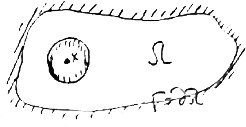
\includegraphics[width=0.2\textwidth]{17_1_new}
\end{center}
В $\Omega_x^\varepsilon$ ядро $K_3(x,y) = - \frac{1}{4\pi \abs{x-y}} \in C^\infty$ ($\Delta K_3(x,y) \equiv 0$). Используем 2 формулу Грина:
\begin{multline*}
\int_{\Omega_x^\varepsilon} \Delta u(y) K_3(x,y)dy - \int_{\Omega_x^\varepsilon} u(y) \Delta K_3(x,y)dy = {}\\
{}=\oint_\Gamma \pd{u(y)}{\vec{n_y}} K_3(x,y)dS_y + \oint_\gamma \pd{u(y)}{\vec{n_y}} K_3(x,y)dS_y - \oint_\Gamma u(y)\pd{}{\vec{n_y}} K_3(x,y) dS_y - \oint_\gamma u(y)\pd{}{\vec{n_y}} K_3(x,y) dS_y
\end{multline*}
\begin{multline*}
\Longleftrightarrow \int_{\Omega_x^\varepsilon} f(y) K_3(x,y)dy + \oint_\Gamma u(y)\pd{}{\vec{n_y}} K_3(x,y) dS_y - \oint_\Gamma \pd{u(y)}{\vec{n_y}} K_3(x,y)dS_y = {}\\
{} = \oint_\gamma \pd{u(y)}{\vec{n_y}} K_3(x,y)dS_y - \oint_\gamma u(y)\pd{}{\vec{n_y}} K_3(x,y) dS_y
\end{multline*}
\begin{offtop}
интеграл от $\frac{1}{\abs{x}^\alpha}$ сходится при $\alpha < n = \mathrm{dim}\, \R^n$. У нас $n=3, \alpha =1$.
\end{offtop}
Устремляем $\varepsilon \rightarrow 0$:
\begin{enumerate}
\item $\int_{\Omega_x^\varepsilon} \rightarrow \int_\Omega$ в силу последнего замечания.
\item
$
\oint_\gamma u(y) \pd{}{\vec{n_y}} \roundBr{-\frac{1}{4\pi} \cdot \frac{1}{|x-y|}}dS_y  = \frac{1}{4\pi \varepsilon^2} \oint \roundBr{u(y) - u(x) + u(x)}dS_y = \frac{1}{4\pi \varepsilon^2} \oint_\gamma \roundBr{u(y) - u(x)}dS_y + u(x)$\\
$\pd{}{\vec{n_y}} \roundBr{-\frac{1}{4\pi} \cdot \frac{1}{|x-y|}} \rightarrow \left.\frac{1}{4\pi}\roundBr{-\pd{}{\rho}\frac{1}{\rho}}\right|_{\rho = \varepsilon}$\\
$\frac{1}{4\pi \varepsilon^2} \abs{ \oint_\gamma \roundBr{u(y) - u(x)}dS_y} \leq \frac{1}{4\pi \varepsilon^2} \cdot \max\limits_{|y-x| \leq R} \abs{u(y)-u(x)} \cdot \oint_\gamma dS_y \rightarrow 0
$
\item
\begin{align*}
&\abs{\oint_\Gamma \pd{u(y)}{\vec{n_y}} K_3(x,y)dS_y} \leq \frac{1}{4\pi \varepsilon} M \int_\gamma dS_y = M \varepsilon \rightarrow 0\\
& \abs{\pd{u}{\vec{n_y}}} = \abs{(\nabla u, \vec n)} \leq \abs{\nabla u} \cdot \abs{n} \leq M, \text{ так как } \nabla u \in C\roundBr{\overline{\Omega}}
\end{align*}
\end{enumerate}
Итак, после предельного перехода получим требуемое соотношение
\end{proof}
\Subsection{Фундаментальное решение уравнения Лапласа.}
Экскурс в обобщенные функции
\begin{definition}
$\mathcal{D}(\R^n)$ -- пространство пробных (основных) функций:\\ $\varphi(x) \in \mathcal{D}(\R^n) \Longleftrightarrow \varphi(x) \in C^\infty(\R^n),\; \mathrm{supp}\, \varphi(x)$ -- компакт. 
\end{definition}
\begin{definition}
В $\mathcal{D}(\R^n)$ вводится сходимость по следующему правилу: $\curlyBr{\varphi_k(x)}_{k=1}^{\infty} \rightarrow \varphi(x) \in \mathcal{D}(\R^n) \Longleftrightarrow$
\begin{itemize}
\item $\forall \alpha = (\alpha_1, \ldots, \alpha_n)\; \mathcal{D}^\alpha \varphi_k \rightrightarrows \mathcal{D}^\alpha \varphi$
\item $\exists A > 0: \varphi_k (x) \equiv 0$ при $|x| > A \Forall k \in \N$ (у всех функций общий носитель)
\end{itemize}
\end{definition}
Пример функции из $\mathcal{D}(\R^n)$: 
$$\omega_\varepsilon(x) = \begin{cases}\frac{1}{\varepsilon^n}e^{-\frac{1}{1-\roundBr{x/\varepsilon}^2}}, |x| \leq \varepsilon \\ 0, |x| > \varepsilon \end{cases} \Rightarrow \mathcal{D}(\R^n) \neq \varnothing$$
\begin{definition}
Обобщенная функция $f$ над $\mathcal{D}(\R^n)$ -- всякий линейный непрерывный функционал над $\mathcal{D}(\R^n)$
\end{definition}
\begin{definition}
Линейный функционал: $(f, \alpha \varphi + \mu \psi) = \alpha (f, \varphi) + \mu (f, \psi)$
\end{definition}
\begin{definition}
Непрерывный функционал: $\forall \curlyBr{\varphi_k} \rightarrow \varphi$ в  $\mathcal{D}(\R^n) \Rightarrow f(\varphi_k)\rightarrow f(\varphi)$
\end{definition}
По определению $\forall \lambda, \mu \text{ -чисел}, \Forall f, g \in \mathcal{D}'(\R^n)$ обобщенная функция $F = \lambda f + \mu g \in \mathcal{D}'(\R^n), \;\\(F, \varphi)  \stackrel{\mathrm{def}}{=} \lambda (f, \varphi) + \mu (g, \varphi)$
\begin{definition}[сходимость в $\mathcal{D}'(\R^n)$]
$\curlyBr{f_n}_{n=1}^\infty \rightarrow f \in \mathcal{D}'(\R^n) \stackrel{\mathrm{def}} {\Longleftrightarrow} (f_k, \varphi) \rightarrow (f, \varphi), \Forall \varphi \in \mathcal{D}(\R^n)$ (слабая$^*$ сходимость). 
\end{definition}
\begin{definition}
Функция $f(x)$ называется локально интегрируемой, если 
$$\forall\: B > 0 \quad \exists \displaystyle\int\limits_{|x| < B} \abs{f(x)}dx < \infty$$
\end{definition}
Каждая такая $f(x)$ порождает обобщенную функцию $(f,\varphi) = \int_{\R^n} f(x) \varphi(x) dx$.\\
Если существует локально интегрируемая $f(x)$ такая, что обобщенная функция $f$ представляется в виде $(f,\varphi) = \int_{\R^n} f(x) \varphi(x) dx$, то $f \in \mathcal{D}'(\R^n) $ называется регулярной.
\begin{lemma}[Дюбуа-Реймон]
Если $f$ и $g$ непрерывны и порождают одну обобщенную функцию, то $f \equiv g$. Если $f$ и $g$ разрывны, то они совпадают почти всюду.
\end{lemma}
\begin{definition}[$\delta$-функция]
$(\delta, \varphi) \stackrel{\mathrm{def}}{=} \varphi(0)$
\end{definition}
$\delta$-функция не является регулярной. \\
Обобщенные функции бесконечно дифференцируемы.\\
Правило дифференцирования: $(\mathcal{D}^\alpha f, \varphi) = (-1)^{|\alpha|} (f, \mathcal{D}^\alpha \varphi)$.\\
В частном случае $(\Delta f, \varphi) = (f, \Delta \varphi)$
\begin{theorem}
Функция $E(x) = \frac{-1}{4\pi |x|}$ является решением в обобщенных функциях уравнения $\Delta E(x) = \delta(x)$.
\end{theorem}
\begin{proof}
Пусть $\varphi \in \mathcal{D}(\R^n), \mathrm{supp} \varphi \subset B(0, A)$. Возьмем $\Omega = B(0, A +1)$. По теореме об интегральном представлении
\begin{align*}
\varphi(0) &= \int_{|y| < A +1} E(y) \Delta_y \varphi(y) dy + \cancel{\oint_{|y| = A+1} \varphi(y)\pd{E(y)}{\vec{n_y}} dS_y} - \cancel{\oint_{|y| = A+1} \pd{\varphi(y)}{\vec{n_y}} E(y)dS_y} = \\
&= (E, \Delta_x \varphi(x)) = (\Delta E, \varphi(x))
\end{align*}
Что и требовалось.
\end{proof}
\begin{definition}
Функция $E(x)$ называется фундаментальным решением оператора Лапласа.
\end{definition}
\newpage
\section{Свойства гармонических функций в $\R^3$: бесконечная дифференцируемость, теорема о среднем. Обратная теорема о среднем.}
% Затехала Ермолова Марина
\begin{definition} Функция $u(x)$ гармоническая в $\Omega \in \R^3$, если 
\begin{enumerate}
\item $u(x) \in C^2 (\Omega)$
\item $\Delta u(x) = 0 \Forall x \in \Omega$ 
\end{enumerate}
\end{definition}
\begin{theorem}
Всякая функция $u(x)$, гармоническая в области $\Omega$, является в $\Omega$ бесконечно дифференцируемой, т.е. $u(x) \in C^{\infty}(\Omega).$
\end{theorem}
\begin{proof}
Возьмем $x_0 \in \Omega$ и $\overline{B}_r(x_0) \subset \Omega$. Представим $u(x)$ суммой: $$u(x)= - \oint\limits_{|y-x_0|=r} \bigg( \frac{-1}{4\pi |x-y|} \bigg) \frac{\partial u(y)}{\partial \vec{n_y}} dS_y + \oint\limits_{|y-x_0|=r} u(y) \frac{\partial}{\partial \vec{n_y}} \bigg(\frac{-1}{4\pi |x-y|}\bigg) dS_y $$
\begin{center}
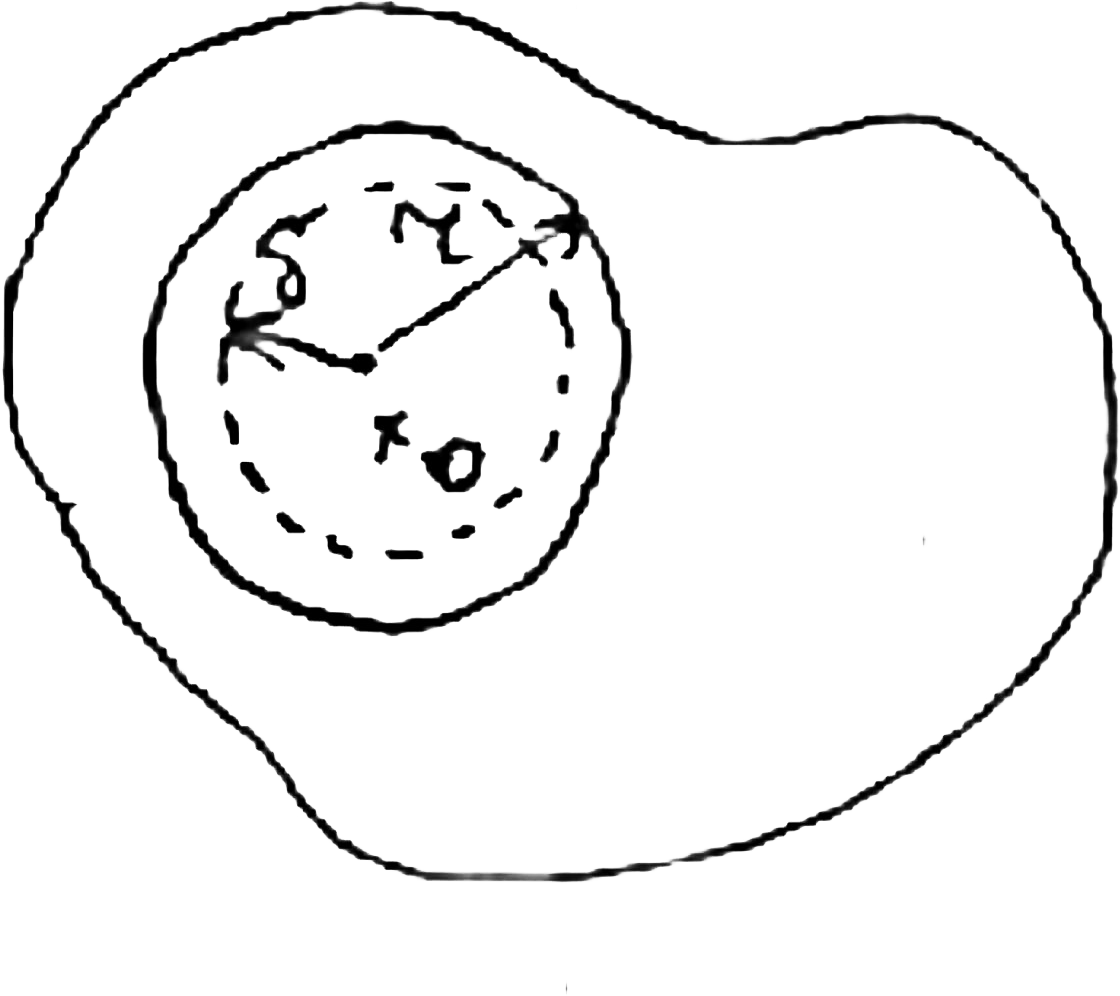
\includegraphics[width=0.2\textwidth]{17_2_new}
\end{center}
Теперь берем $B_{\delta}(x_0) \subsetneq B_{r}(x_0).$ Будем обозначать $S(x_0,r)$ сферу $\partial B_r(x_0).$ Если $x \in \overline{B}_{\delta}(x_0), y \in S(x_0,r)$, то $|x-y| \geq r - \delta > 0.$\\
Рассмотрим в $\overline{B}_{\delta}(x_0)$ $$u_0(x)= \oint\limits_{|y-x_0|=r} \bigg( \frac{-1}{4\pi |x-y|} \bigg) \frac{\partial u(y)}{\partial \vec{n_y}} dS_y.$$
Напишем $$\tilde{u_0}(x) = \oint\limits_{|y-x_0|=r} D_x^\alpha \bigg( \frac{-1}{4\pi |x-y|} \bigg) \frac{\partial u(y)}{\partial \vec{n_y}} dS_y$$
Заметим, что $\frac{-1}{4\pi |x-y|} \in C^{\infty}( \overline{B}_{\delta}(x_0) \times S(x_0,r)) \Rightarrow$ записанные частные производные непрерывны, интеграл $\tilde{u_0}$ существует $\Rightarrow \tilde{u_0}(x) = D_x^\alpha u_o(x).$\\
Теперь берем $$u_2(x) = \oint\limits_{|y-x_0|=r} u(y) \frac{\partial}{\partial \vec{n_y}} \bigg(\frac{-1}{4\pi |x-y|}\bigg) dS_y$$ 
$$\frac{\partial}{\partial \vec{n_y}} \bigg(\frac{-1}{4\pi |x-y|}\bigg) = \sum_1^n n_k \frac{\partial}{\partial \vec{y_k}} \bigg(\frac{-1}{4\pi |x-y|}\bigg)$$ В $\overline{B}_{\delta}(x_0)$ запишем 
$$\tilde{u_2}(x)=\sum_1^3 \oint u_0(y) n_k (y) D_x^\alpha \bigg(\frac{\partial}{\partial \vec{y_k}} \bigg(\frac{-1}{4\pi |x-y|}\bigg)dS_y$$
Записанные частные производные непрерывны, интеграл $\tilde{u_2}(x)$ существует $\Rightarrow \tilde{u_2}(x)=D_x^\alpha u_2(x).$\\
Итак, для $u_0(x)$ и $u_2(x)$ существуют частные производные любого порядка. Значит, $u(x) \in  C^{\infty}( \overline{B}_{\delta}(x_0)),$ где\\ $x_0$ - произвольная точка из $\Omega. \Rightarrow u(x) \in C^{\infty}(\Omega)$
\end{proof}
\begin{theorem}[Теорема о среднем]
Пусть $u(x)$, гармоническая в шаре $B_r(x_0)$ и $u(x) \in C^1(\overline{B}_r(x_0))$. Тогда $u(x_0)= \frac{1}{4\pi r^2} \int \limits_{|y-x_0|=r}u(y)dS_y.$ (в центре - среднее по значениям на сфере)
\end{theorem}
\begin{proof}
$$u(x_0)= -\oint\limits_{|y-x_0|=r} \bigg( \frac{-1}{4\pi |x_0-y|} \bigg) \frac{\partial u}{\partial \vec{n_y}} dS_y + \oint\limits_{|y-x_0|=r} u(y) \frac{\partial}{\partial \vec{n_y}} \bigg(\frac{-1}{4\pi |x_0-y|}\bigg) dS_y $$
$$\frac{\partial}{\partial \vec{n_y}} \bigg(\frac{-1}{4\pi |x_0-y|}\bigg)\stackrel{\rho = |x_0 - y|}{=} \frac{-1}{4\pi}\frac{\partial}{\partial \rho}\frac{1}{\rho} = \frac{1}{4 \pi r^2},$$ тогда $$\oint\limits_{|y-x_0|=r} u(y) \frac{\partial}{\partial \vec{n_y}} \bigg(\frac{-1}{4\pi |x_0-y|}\bigg) dS_y = \frac{1}{4 \pi r^2} \oint\limits_{|y-x_0|=r} u(y) dS_y.$$
Покажем, что потенциал простого слоя равен нулю.
\[ -\oint\limits_{|y-x_0|=r} \bigg( \frac{-1}{4\pi |x_0-y|} \bigg) \frac{\partial u(y)}{\partial \vec{n_y}} dS_y = \frac{1}{4\pi} \frac{1}{r} \oint\limits_{|y-x_0|=r}  \frac{\partial u(y)}{\partial \vec{n_y}} dS_y = \frac{1}{4\pi r} \oint\limits_{|y-x_0|=r} (\nabla u(y), \vec{n}(y)) dS_y \stackrel{\text{ф-ла Остр.-Гаусса}}{=}
\]
\[
 = \frac{1}{4\pi r} \oint\limits_{|y-x_0|<r} \div(\nabla u) dy = \frac{1}{4\pi r} \oint\limits_{|y-x_0|<r} \Delta u dy  = 0
 \]
\end{proof}
\begin{theorem}[Обратная теорема о среднем]
Пусть $u(x) \in C(\Omega)$ и $u(x)$ обладает свойством среднего $\forall x \in \Omega$, где $\Omega \in \R^3$ - произвольная область. Тогда $u(x)$ - гармоническая функция на $\Omega$. 
\end{theorem}
\begin{proof}
$\forall x_0\in\Omega\Exists r > 0: \overline{B(x_0, r)}\subset\Omega.$ 
Рассмотрим решение $$v(x) = \frac{1}{4\pi R}\oint\limits_{|y|=r}\frac{r^2-|x|^2}{|y-x|^3}u(y)dS_y $$ 
$$\text{для задачи} \begin{cases}
\Delta u(x) = 0, |x| < r \\
\eval{v}_{|x| = r} = \eval{u}_{|x| = r}
\end{cases} $$
Введем $w(x) = u(x) - v(x)$, $w(x) \in C(|x| \leq r)$, получим что $w(x)$ удовлетворяет свойству среднего. Тогда по принципу максимума (для функции, удовлетворяющей свойству среднего, будет доказан в следующем билете) $|w(x)| \leq \max\limits_{|y-x| = r}|w(y)| = 0  \Rightarrow u(x) = v(x) \Forall x\colon |x| < r$
\end{proof}
\newpage

\section{Билет 19.Принцип максимума и минимума для гармонических функций. Единственность классического решения задачи Дирихле для уравнения Пуассона при непрерывной граничной функции}
%Никитушка отмочил красоту
\subsection{Теорема (принцип максимума)}
\begin{theorem}
{\bf(Принцип максимума)} Если $u(x)$ - гармоническая в
области $\Omega$ и достигает $max$ или $min$ значения в
точке $a \in \Omega$, то $u(x) \equiv u(a) \Forall x \in \Omega$ 

\begin{offtop}
Теорема справедлива в $\R^n$
\end{offtop}

\begin{proof}

\begin{itemize}
\item
\item 
Докажем вспомогательное локальное 
\begin{statement}
\label{statement_19.1}
Пусть $u(x) \in C^2(\Omega)$ достигает максимума в точке $a$, а так же удовлетворяет {\bf свойству среднего}:

\[
u(a) = \dfrac{1}{4\pi r^2}\oint\limits_{\abs{y-a} = r}u(y
)\;dS_y \Forall r: 0 < r < d_a = dist(a, \R^3 \backslash
 \Omega)
\]

Тогда $u(x) \equiv u(a) \Forall x \in B(a, d_a)$  

\end{statement}
\begin{proof}
$
u(a) = \dfrac{1}{4\pi r^2}\oint\limits_{\abs{y-a} = r}u(y
)\;dS_y  =
\dfrac{u(a)}{4\pi r^2}\oint\limits_{\abs{y-a} = r} \;dS_y  +
 		\dfrac{1}{4\pi r^2}\oint\limits_{\abs{y-a} = r}\roundBr{u(y
)-u(a)}\;dS_y =
	u(a) + \dfrac{1}{4\pi r^2}\oint\limits_{\abs{y-a} = r}\roundBr{u(y
)-u(a)}\;dS_y \Rightarrow 
	\oint\limits_{\abs{y-a} = r}\underbrace{\roundBr{u(y)-u(a)}}_{\le 0,\ \text{непрерывна}}\;dS_y = 0
	 \Leftrightarrow
	\quad u(y) = u(a) \Forall y: |y-a|=r < d_a
 $
\end{proof}

\item
{\bf Докажем саму теорему}
\begin{center}
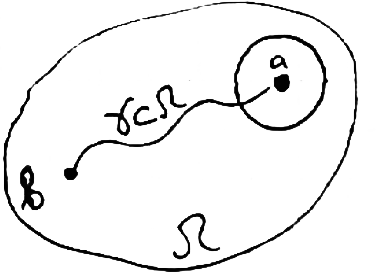
\includegraphics[scale=0.5]{19_1_new}
\end{center}
Соединим $a$ и $b$ кусочно-гладкой кривой. Эту кривую параметризуем натуральным параметром(параметризация кривой длиной её дуги): 
$x = x(s), x(0) = a, x(L) = b$.
{\bf Обозначим}
$d = dist\curlyBr{\gamma = x; \partial{\Omega}} > 0$
($d$ действительно $> 0$ : если $d = 0$, то 
$\exists\{x_n\}_{n=1}^\infty \subset \gamma: \rho\roundBr{x_n, \partial\Omega}\to 0$.
 Выделим из $\{x_n\}$ сходящуюся $\{x_{n_k}\}=\{y_k\}$($\gamma$ - ограничено). Пусть $y_k \to y_0$. Тогда $y_0$ - предельная для
 $\partial \Omega$ в силу замкнутости 
 $y_0 \in \gamma \cup \partial \Omega \Rightarrow$ противоречие)\\
 Разобьем $[0,L]$ на части размера $\Delta S = \dfrac{L}{N}$\\
 Пусть $\curlyBr{S_k = k\Delta S, x_k = x(S_k)}$. 
 Число N выберем так, чтобы $\Delta S = \dfrac{L}{N} < d$\\
 \begin{center}
 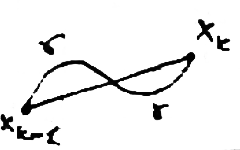
\includegraphics[scale=0.5]{19_2_new}
 \end{center}
 Заметим, что $\abs{x_k - x_{k-1}} \boxed{\leq} s_k - s_{k-1} < d$($\boxed{\cdot}$ - кратчайшее расстояние между точками это отрезок).
 \begin{center}
 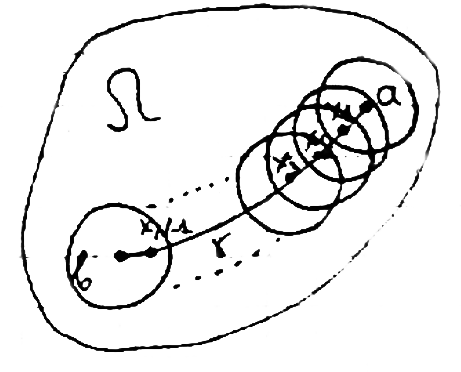
\includegraphics[scale=0.5]{19_3_new}
\end{center}
 Рассмотрим шары ${B_d(x_k)}_{k=0}^N$. В силу
 $\abs{x_k - x_{k-1}}) < d$ верно $x_{k+1} \in B_d(x_k)$. 
  Примем утверждение \ref{statement_19.1} к первому шару. 
  Как следствие $u(x_1) = u(a)\Rightarrow$ утверждение \ref{statement_19.1} применимо уже ко второму шару.
   В цепочке шаров конечное число 
  $\Rightarrow$ добираемся до точки $b$ - теорема доказана.  
\end{itemize}
\end{proof}
\end{theorem}

$\bullet$ Заметим, что достаточно было потребовать
свойство среднего и непрерывность, вместо гармоничности.


\begin{conseq}
\label{conseq19.1}
Пусть $\Omega$ - ограниченная область, а $u(x)$ - гармоническая в $\Omega$ и непрерывная на $\overline{\Omega}$.
Тогда $u(x)$ достигает $max$ и $min$ на $\partial \Omega$, т.е.
$\min\limits_{y \in \partial \Omega}u(y) \leq u(x) \leq \max\limits_{y \in \partial \Omega}u(y)$
	\begin{proof}
	Либо максимум/минимум на границе, либо $u(x)\equiv const$ в $\Omega$
	\end{proof}
\end{conseq}


\begin{conseq}
Для указанной в следствии \ref{conseq19.1} $u(x) \hookrightarrow \abs{u(x)} \leq \max\limits_{y \in \partial \Omega} \abs{u(y)}$
\begin{proof}

\begin{equation}
  \begin{cases}
  & u(x) \leq \max\limits_{\partial \Omega}u(y) \leq \max\limits_{\partial \Omega}\abs{u(y)}\\  
  &-u(x) \leq \max\limits_{\partial \Omega}(-u(y)) \leq \max\limits_{\partial \Omega}\abs{u(y)}\\
  \end{cases}
  \end{equation}  
  
  $\Rightarrow \abs{u(x)} \leq \max\limits_{\partial \Omega}\abs{u(y)}$
\end{proof}
\end{conseq}


\subsection{Новая постановка задачи Дирихле для уравнения Пуассона}
$\Omega$ - ограниченная область 

\begin{equation}
  \begin{cases}\label{equatation19.1}
  & \Delta u(x) = f(x), x \in \Omega\\ 
  & \while{u(x)}{\partial \Omega} = u_0(x), x \in \partial \Omega\\
  \end{cases}
\end{equation} 
  
 \begin{definition}
 Классическое решение задачи Дирихле - функция
  $u(x) \in C^2(\Omega) \cap C(\overline{\Omega})$,
  удовлетворяющая уравнению и граничному условию.(раньше было $u(x) \in C^2(\Omega) \cap C^{\boxed{1}}(\overline{\Omega})$, единица была нужна для формул Грина, теперь убираем ее)
 \end{definition}
 \subsection{Теорема единственности}
 \begin{theorem}
 (единственности) Не может существовать более 1 классического решения задачи Дирихле(\ref{equatation19.1}).
 
 \begin{proof}
 Пусть $u_1$ и $u_2$ - классические решения (\ref{equatation19.1}). Тогда $v(x) = u_1 - u_2$ - классическое решение полностью однородной задачи:
 
 \begin{equation}
  \begin{cases}\label{equatation19.2}
  & \Delta v(x) \equiv 0, x \in \Omega\\ 
  & \while{v(x)}{\partial \Omega} = 0, x \in \partial \Omega\\
  \end{cases}
\end{equation}
 
 Согласно принципу максимума, $\abs{v(x)} \leq \max\limits_{\partial\Omega} \abs{v(x)} = 0 \Rightarrow v(x) \equiv 0$
 \end{proof}
 \end{theorem}
\newpage
\section{Функция Грина для задачи Дирихле (случай $\R^3$). Функция Грина для шара. Формула Пуассона решения задачи Дирихле для уравнения Лапласа в шаре}
% Затехал: Дмитрий Федоряка

\Subsection{Функция Грина}
Пусть $\Omega \subset \R^3$ - ограниченная область с кусочно-гладкой границей.

Пусть $u(x) \in C^2(\Omega) \cap C^1(\overline{\Omega})$ --- некоторое классическое решение задачи:

\[\begin{cases}
   \triangle u = f(x), & x\in \Omega \\
   \while{u}{\partial \Omega} = u_0(x), & x \in \partial \Omega  
\end{cases}\]  

Запишем интегральное представление:

$$ u = \int_{\Omega}{\roundBr{\frac{-1}{4 \pi |x-y|}}  {\triangle u(y)} dy} - \oint_{\partial \Omega}{\roundBr{\frac{-1}{4 \pi |x-y|}} \frac{\partial u(y)}{\partial \overrightarrow{n}_y} d S_y} + 
\oint_{\partial \Omega}{ {u(y)} \frac{\partial}{\partial \overrightarrow{n}_y}\roundBr{\frac{-1}{4 \pi |x-y|}}d S_y}
$$

Рассмотрим задачу при фиксированном $x \in \Omega$:

\[\begin{cases}
   \triangle_y g(x,y) = 0, & \Forall y \in \Omega \\
   g(x,y)|_{\partial \Omega} = \frac{1}{4 \pi |x-y|}  
\end{cases}\] 

Если $\partial \Omega \in C^2$, то решение существует (пока не можем это доказать).

Используем вторую формулу Грина:

$$ \int_{\Omega}{\triangle_y u(y) g(x,y)dy} - 
{\underset{=0}{\int_{\Omega}{u(y) \triangle_y g(x,y) dy}}}=$$

$$=\oint_{\partial \Omega} {\frac{\partial u(y)}{\partial \overrightarrow{n}_y} g(x,y) dS_y} - \oint_{\partial \Omega} {\frac{\partial g(x,y)}{\partial \overrightarrow{n}_y} u(y) dS_y} $$

Отсюда получаем

$$\int_{\Omega}{g(x,y) f(y) dy} + \underset{wanted~to~find}{\oint_{\partial \Omega}{\roundBr{\frac{-1}{4 \pi |x-y|}} \frac{\partial u(y)}{\partial \overrightarrow{n}_y} d S_y}}+ \oint_{\partial \Omega}
{\frac{\partial g(x,y)}{\partial \overrightarrow{n}_y}u(y) dS_y} = 0
$$

Тогда

$$u(x) = \int_{\Omega} {\roundBr{\frac{-1}{4 \pi |x-y|} +g(x,y)} f(y) dy} + \oint_{\partial \Omega} {u_0(y) \frac{\partial}{\partial \overrightarrow{n}_y} \roundBr{\frac{-1}{4 \pi |x-y|}+g(x,y)}dS_y}
$$

\textbf{Функция Грина}, по определению:

$$G(x,y) \triangleq  \frac{-1}{4 \pi |x-y|} + g(x,y) $$

Она симметрична и имеет ту же особенность, что и $\frac{-1}{4 \pi |x-y|}$





\Subsection{Функция Грина для шара}


Получим функцию Грина для шара:
\[\begin{cases}
   \triangle_y g(x,y) = 0, y \in \Omega \\
   g(x,y)|_{|y|=R} = \frac{1}{4 \pi |x-y|}& 
\end{cases}\]  

Будем обозначать $x^*$ точку, инверсную точке $x$ относительно окружности $|y|=R$.
$$x^* = x \frac{R^2}{|x|^2}$$
\begin{center}
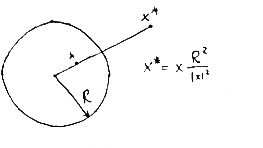
\includegraphics{20_1_new}
\end{center}
Покажем, что решением является функция:

\[g(x,y) = \begin{cases}
   \frac{R}{4 \pi |x| |y-x^*|},   & x \ne 0 \\
   \frac{1}{4 \pi R},& x=0
\end{cases}\]

Функция $g(x,y)$ - гармоническая по $y$ в шаре $|y|<R$ (особенность $y=x^*$ лежит вне шара, т.к. $x*$ лежит внутри него).

Посмотрим значение функции $g$ на границе:
\begin{center}
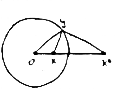
\includegraphics{20_2_new}
\end{center}
Заметим, что $\triangle OXY \sim \triangle OYX*$, т.к. $\angle XOY$- общий, и $\frac{|x|}{|y|}  =\frac{|y|}{|x^*|}$.

Из подобия $\frac{|y-x|}{|y-x^*} = \frac{|x|}{|y|} = \frac{|x|}{R}$.

Значит, $\left.\frac{R}{4 \pi |x| |y-x^*|} \right|_{|y|=R} = \frac{1}{4 \pi y}$, что и требовалось.

\Subsection{Формула Пуассона в шаре}

Получим формулу Пуассона решения задачи Дирихле в шаре:

$$u(x) = \int_{\Omega}{G(x,y) \underset{=0}{f(y)} dy} +
\oint_{\partial \Omega}{u_0(y) \frac{\partial G(x,y)}
{\partial \overrightarrow{n}_y}dS_y}
$$
Преобразуем последний интеграл:\\

$
\frac{\partial G(x,y)}{\partial \overrightarrow{n}_y}=
\sum_{k=1}^{3}{n_k(y) \left. \frac{\partial G}{\partial y_k} \right|_{|y|=R}}=
\sum_{k=1}^{3}{n_k(y)\frac{\partial}{\partial y_k}\left[
-\frac{1}{4\pi}\left(\frac{1}{|y-x|}-\frac{R}{|x|}\frac{1}{|y-x^*|}\right)
\right]} 
=
\frac{1}{4 \pi}  \sum_{k=1}^{3}\underset{=n_k(y)}{\frac{y_k}{R}}\left[ \frac{y_k-x_k}{|y-x|^3} - \frac{R}{|x|}  \frac{y_k-x_k^*}{|y-x^*|^3} \right]
$\\

Вспомним, что $\left.\frac{R}{|x|\cdot|y-x^*|}\right|_{|y|=R} =
\frac{1}{|x-y|}$:

$$
\left. \frac{\partial G(x,y)}{\partial \overrightarrow{n}_y} \right|_{|y|=R} 
=
\sum_{k=1}^{3}{\frac{1}{4 \pi} \frac{y_k}{R}
\left[ \frac{y_k-x_k}{|y-x|^3} -\frac{R}{|x|}\roundBr{\frac{|x|}{R}}^3
\frac{y_k - x_k^*}{|y-x|^3} \right] }
=
\frac{1}{4 \pi R |y-x|^3} \sum_{k=1}^{3}{y_k \squareBr{y_k-x_k-\frac{|x|^2}{R^2}(y_k - x_k^*)}}
=
$$

$$
=
\frac{1}{4 \pi R |y-x|^3} \squareBr{\angleBr{y,y-x} - \frac{|x|^2}{R^2}
\angleBr{y,y-x^*}}
=
\frac{1}{4 \pi R |y-x|^3} \squareBr{\underset{=R^2}{\angleBr{y,y}} - \angleBr{y,x}
-\frac{|x|^2}{R^2}\underset{=R^2}{\angleBr{y,y}}+ \underset{=\angleBr{y,x}}{\frac{|x|^2}{R^2} \angleBr{y,x^*}}  }
= $$ 
$$
=\frac{R^2 - |x|^2}{4 \pi R |y-x|^3}
$$

Итак, \textbf{формула Пуассона для решения задачи Дирихле для уравнения Лапласа в шаре}:

$$
u(x) = \frac{1}{4 \pi R} \oint_{|y|=R}{\frac{R^2-|x|^2}{|y-x|^3}u_0(y) dS_y}
$$



\newpage
\section{Билет 21. Теорема Лиувилля для гармонических функций (случай $\R^3$)}
% Затехал: Дмитрий Федоряка

\subsection{Формулировка теоремы} 

\begin{theorem}

{\bf (Теорема Лиувилля)} Функция $u(x)$, гармоническая в $\R^3$ ($\Delta u = 0$)  и имеющая на бесконечности рост не выше степенного (т.е. $|u(x)| \le C (1+|x|)^{\mu}$), является многочленом от $x_1,x_2,x_3$ степени не выше $\mu$.

\end{theorem}

\subsection{Доказательство при $\mu \ge 0$}

Общая идея - доказать, что все производные степени выше $\mu$ равны нулю.


\begin{enumerate}



\item{

Выберем $x \in \R^3, R>0$ так, чтобы $R > 2|x|$:
\begin{center}
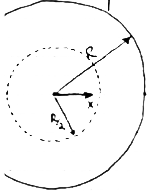
\includegraphics{21_1_new}
\end{center}
В области $|x|<R$ $u(x)$ - гармоническая, а $\left. u(x) \right|_{\partial \Omega} \in C(\partial \Omega)$.

Тогда применима формула Пуассона для шара:

$$u(x) = \frac{1}{4 \pi R} \oint_{|y|=R}{\frac{R^2-|x|^2}{|y-x|^3} u(y) dS_y }
$$

В силу выбора $R$ имеем $|y-x| \ge |y|- |x| \ge \frac{R}{2} >0$.

Можем записать:

$$\mathcal{D}_{x}^{\alpha} u(x) = \frac{1}{4 \pi R} 
\oint_{|y|=R}{\mathcal{D}_{x}^{\alpha}\brs{\frac{R^2-|x|^2}{|y-x|^3}}u(y) dS_y}$$

}





\item{

Докажем по индукции, что
 
$$\forall \alpha = (\alpha_1,\alpha_2,\alpha_3)~~~ \mathcal{D}_{x}^{\alpha}\sbrs{\frac{R^2-|x|^2}{|x-y|^3}} = \frac{P_{\alpha}(R,x,y)}{|x-y|^{3+2|\alpha|}},$$

где $P_\alpha$ - однородный многочлен степени $|a|+2$ от $R, x_1,x_2,x_3,y_1,y_2,y_3$.


\begin{itemize}
	\item {База:}
	
	$$\mathcal{D}_{x}^{(0,0,0)}\sbrs{\frac{R^2-|x|^2}{|x-y|^3}} = \frac{R^2-x_1^2-x_2^2-x_3^2}{|x-y|^3}$$
	
	\item {Переход. 
Пусть требуемое верно $\forall \alpha: |a|\le k$. Возьмём $\hat{\alpha}=(\alpha_1+1, \alpha_2, \alpha_3)$:}

$$
\mathcal{D}_{x}^{\hat{\alpha}}\sbrs{\frac{R^2-|x|^2}{|x-y|^3}} = \frac{\partial}{\partial x_1}
\sbrs{\frac{P_{\alpha}(R,x,y)}{|x-y|^{3+2|\alpha|}}}
=
\frac{
\frac{\partial P_{\alpha}}{\partial x_1} \cdot |x-y|^2 - (3+2|\alpha|)\cdot P_\alpha \cdot (x_1-y_1)
}
{|x-y|^{3+2(|\alpha|+1)}}
=
\frac{P_{\hat{\alpha}}(R,x,y)}{|x-y|^{3+2|\hat{\alpha}|}}
$$ 
	
\end{itemize}
}



\item{
Покажем теперь, что $\forall |x| \le \frac{R}{2}, \forall |y|=R, \forall \alpha =(\alpha_1,\alpha_2,\alpha_3)$ справедлива оценка:

$$\left| \mathcal{D}_{x}^{\alpha}\brs{\frac{R^2-|x|^2}{|x-y|^3}} \right| \le \frac{C_\alpha}{R^{1+|\alpha|}}.
$$

Действительно, $|P_\alpha| \le \tilde{C}_\alpha R^{|a|+2}$, а $|x-y|^{3+2|\alpha|} \ge \brs{\frac{R}{2}}^{3+2|\alpha|} = \hat{C_\alpha}R^{3+2|\alpha|}$. Отсюда следует требуемая оценка.
}

\item{

Теперь докажем, что $\mathcal{D}_x^\alpha u(x) = 0 ~~ \forall \alpha: |\alpha|>\mu$.

$$
\left| \mathcal{D}_x^{\alpha} u(x) \right| = \frac{1}{4 \pi R} 
\left|
\oint_{|y|=R}{\mathcal{D}_x^{\alpha}\brs{\frac{R^2-|x|^2}{|y-x|^3}}u(y)dS_y}
\right|
\le
\frac{1}{4 \pi R} \cdot C \cdot (1+ |x|)^\mu \cdot 
\frac{C_\alpha}{R^{1+|a|}} \cdot 4 \pi R^2 
\le$$ 
$$
\le
\frac{C \cdot C_\alpha \cdot (1+R)^\mu}{R^{|\alpha|}} 
\underset{R \to \infty}{\longrightarrow}
0 ~~
\text{Значит,}~~ \mathcal{D}_x^{\alpha} u(x)=0~ \forall x \in \R^3, |\alpha|>\mu .$$

} 


\item{

Для гармонической в $\R^3$ функции $u(x)$ справедливо представление:

$$
u(x) = u(0) + \sum_{k=1}^{m} \sum_{|\alpha|=k} \frac{1}
{\alpha_1! \alpha_2! \alpha_3!} \mathcal{D}_x^{\alpha} u(0) 
x_1^{\alpha_1}x_2^{\alpha_2}x_3^{\alpha_3}
+
\sum_{k=m+1}^{\infty} \sum_{|\alpha|=k} \frac{1}
{\alpha_1! \alpha_2! \alpha_3!} \underset{=0}{\mathcal{D}_x^{\alpha} u(0)}
x_1^{\alpha_1}x_2^{\alpha_2}x_3^{\alpha_3}
=
$$

$$
=
u(0) + \sum_{k=1}^{m} \sum_{|\alpha|=k} \frac{1}
{\alpha !} \mathcal{D}_x^{\alpha} u(0) 
x^{\alpha},
$$

где $m = [\mu], \alpha ! \triangleq \alpha_1!\alpha_2!\alpha_3!, x^\alpha \triangleq x_1^{\alpha_1}x_2^{\alpha_2}x_3^{\alpha_3}$.



}

\end{enumerate}






\subsection{Доказательство при $\mu < 0$}

Пусть $\mu<0$. Тогда т.к. $|u(x)|\le C(1+|x|)^\mu, \mu<0$, то
$|u(x)| \le C (1+|x|)^0 \equiv C_1$. 

По предыдущему пункту, $u(x)$ - полином степени 0, т.е. константа.

Но $|u(x)| \le \frac{C}{(1+|x|)^{|\mu|}} \Rightarrow u(x) 
\underset{|x| \to \infty}{\longrightarrow}
0   \Rightarrow u(x) \equiv 0$.
 

\newpage
\section{Теорема об устранимой особой точке для гармонических функций (случай $\R^3$)}
% Затехал: Дмитрий Федоряка
 

\begin{theorem}

{\bf (об  устранимой особой точке).} 
Пусть $u(x)$ - гармоническая в $\mathring{B}_\rho(a) \subset 
\R^3$ и $u(x)=o(E(x-a))$ при $x \to a$, где $E(x) = -\frac{1}{4 \pi |x|}$. Тогда $u(x)$ можно так доопределить в точке $a$, что она будет гармонической в $B_\rho(a) = \{x: |x-a|<\rho \}$.

\end{theorem}

\textbf{Доказательство.}


\begin{enumerate}
\item{ 
	
	$u(x) = o \roundBr{\frac{1}{|x|}} \Leftrightarrow |x| \cdot u(x) 
	\underset{x \to 0}{\longrightarrow} 0$
}

\item{
Возьмём $r<\rho$. 
\begin{center}
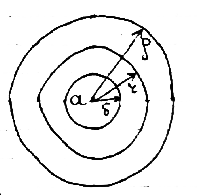
\includegraphics{22_1_new}
\end{center}
Функция $u(x)$ непрерывна на $\partial B_r (a)$.

Построим гармоническую функцию:

$$\hat{u}(x) = \frac{1}{4 \pi r} 
\oint_{|y|=r}\frac{r^2 - |x|^2}{|y-x|^3} u(y) dS_y \in 
C(|x| \le r)$$.

}


\item{

Считаем $a=0$. Покажем, что $u(x) \equiv \hat{u}(x)$ при $0<|x|\le r$. Строим $v(x) = u(x) - \hat{u}(x)$. Эта функция гармоническая в $\mathring{B}_r(a)$, непрерывная на $(0<|x| \le r)$, а также 
$v(x) \equiv 0 \Forall x: |x|=r$ и $|x| \cdot v(x) \underset{x \to 0}{\longrightarrow} 0$. 
 
}

\item{

Фиксируем $\varepsilon >0$ и рассмотрим функции $W_\eps^{\pm} =
\frac{\varepsilon}{|x|} \mp v(x)$.

Функции $W_\eps^{\pm}$ также гармонические в $(0<|x|<r)$, непрерывны на $(0<|x| \le r)$, а 
$\left.W_\eps^{\pm}(x) \right|_{|x|=r} =\frac{\eps}{|x|} >0$.
}

\item{

Выберем $\delta > 0 $ так, чтобы $\forall x:~~ |x| \le \delta \to |x| \cdot |v(x)| < \frac{\varepsilon}{2}$.

При $|x|\le \delta$: 

$$
W_\varepsilon^{\pm} = \frac{\eps}{|x|} \mp v(x) \ge 
\frac{\eps}{|x|} - |v(x)|
\ge 
\frac{\eps}{|x|}\squareBr{1 - \frac{|x|\cdot |v(x)|}{\varepsilon}}
\ge
\frac{\eps}{|x|}\squareBr{1-\frac{1}{2}}
=
\frac{\varepsilon}{2|x|} >0
$$
}



\item{

При $\delta \le |x| \le r$  функции $W_\eps^{\pm}(x)$
 --- гармонические в $(\delta < |x| < r)$ и непрерывны на замыкании 
этой ограниченной области $\Rightarrow$ по принципу максимума 
максимум и минимум достигаются на границе.

Значит, $W_\varepsilon^{\pm} (x) > 0$ при $\delta \le |x| \le r$.

Итак, $W_\varepsilon^\pm(x)$ положительна в $(0<|x| \le r)$
$\Rightarrow$  $|v(x)| < \frac{\varepsilon}{|x|}$ в $(0<|x|\le r)$.

Значит, $v(x) \equiv 0$ при $0<|x|\le r$ $\Rightarrow$ $v(x)$ можно продолжить на $|x|\le r$, положив $v(0)=0$, ч.т.д. 

}

\end{enumerate}



\newpage
\section{Преобразование Кельвина и его свойства. Регулярность поведения гармонических функций на бесконечности. Единственность решения внешних задач Неймана и Дирихле для уравнения Лапласа (случай $\R^3$).}
% Затехал: Ермолова Марина, Иваныч
Пусть $x$ лежит в окрестности $\infty$, т.е. $|x|>R>0$, а $y$ лежит в окрестность нуля. Считаем $y \neq 0.$ Тогда между этими окрестностями есть биекция - инверсия:
$x^*=x \frac{R^2}{|x|^2},x=x^* \frac{R^2}{|x^*|^2}; |x||x^*|=R^2 $
\begin{lemma}
Если функция $u(x)$ гармоническая в окрестности $\infty: \ |x|>R$ в $\R^n$, то функция $u^*(y)= \big(\frac{R}{|y|}\big)^{n-2}\cdot u(\frac{R^2}{|y|^2} y\big)$ будет гармонической в проколотой окрестности нуля. Если $u^*(y)$ гармоническая в проколотой окрестности нуля, то $u(x)= \big(\frac{R}{|x|}\big)^{n-2}\cdot u^*(\frac{R^2}{|x|^2} x\big)$-гармоническая в окрестности $\infty$.
\end{lemma}
\begin{definition}
Преобразование $u(x) \longmapsto u^*(y)$ и $u^*(y) \longmapsto u(x)$ называется \textbf{преобразованием} Кельвина.
\end{definition}
\begin{proof}
Пусть $x \in U_\varepsilon(\infty), y \in U_\delta(0), |x|=\rho, |y|=r, x=y \frac{R^2}{|y|^2}.$\\
Перейдем в сферическую систему. Лемму докажем в одну сторону.\\
$x=(x_1,x_2,x_3)\\
y=(y_1, y_2, y_3).$
\[
\begin{cases}
x_1 = \rho \sin \theta \cos \varphi\\
x_2 = \rho \sin \theta \sin \varphi\\
x_3 = \rho \cos \theta
\end{cases}, 
\begin{cases}
y_1 = r \sin \theta \cos \varphi\\
y_2 = r \sin \theta \sin \varphi\\
y_3 = r \cos \theta
\end{cases}
\]


Тогда $\hat u^*(r, \theta, \phi) = \frac{R}{r}\hat u(\frac{R^2}{r}, \theta, \phi)$:
$$
\widehat{\Delta_y u^*}(r, \theta, \phi) = \brk[s]*{\frac{1}{r}\pdd{}{r}(r\hat u^*(r, \theta, \phi)) + \frac{1}{r}\underbrace{\Delta'_{\theta, \phi}}_{\substack{\text{оп-р Лапласа}\\\text{-Бельтрани}}}\hat u^*(r, \theta, \phi)} = \frac{R}{r} \pdd{}{r}\brk[s]*{\hat u(\underbrace{\frac{R^2}{r}}_{\rho}, \theta, \phi)} + \frac{R}{r^3}\Delta'_{\theta, \phi} \hat u(\underbrace{\frac{R^2}{r}}_{\rho}, \theta, \phi)
$$

Вспомогательная выкладка:

\begin{align*}
    & \pd{}{r} \hat u(\rho, \theta, \phi) = \pd{\hat u}{\rho}\pd{\rho}{r} = -\frac{\rho^2}{R^2}\pd{}{\rho} \hat u(\rho, \theta, \phi) \\
    & \pd{}{r} \hat u(\rho, \theta, \phi) = \pd{}{r} \brk[s]*{-\frac{\rho^2}{R^2}\pd{}{\rho}\hat u(\rho, \theta, \phi)} =
    \frac{\rho^2}{R^4} \pd{}{\rho}\brk[s]*{\rho^2 \pd{}{\rho}\hat u(\rho, \theta, \phi)}
\end{align*}

С учетом выкладки имеем:
$$
\widehat{\Delta_y u^*}(r, \theta, \phi) = \frac{\rho^3}{R^5}\pd{}{\rho} \brk[s]*{\rho^2 \pd{}{\rho}\hat u(\rho, \theta, \phi)} +
\frac{\rho^3}{R^5}\Delta'_{\theta, \phi}\hat u(\rho, \theta, \phi)=\frac{\rho^5}{R^5} \Delta_x \hat u(\rho, \theta, \phi) = 0
$$

\end{proof}

\begin{theorem}
Пусть $u(x)$ -- гармоническая функция в окрестности бесконечности $|x| > R$ и $u(x) \rightarrow 0, x \rightarrow \infty$. Тогда $u(x) = O\roundBr{\frac{1}{|x|}}$ и $D^\alpha u(x) = O\roundBr{\frac{1}{|x|^{1+|\alpha|}}}$ при $x\rightarrow \infty$
\end{theorem}
\begin{proof}
Применим к нашей функции прямое преобразование Кельвина: $u^*(y) = \frac{R}{|y|}u\roundBr{\frac{R^2}{|y|^2}y}$. Эта функция гармоническая в проколотой окрестности нуля: $0 < |y| < R$.\\
Далее, $|y|u^*(y) = R u\roundBr{\frac{R^2}{|y|^2}y} \rightarrow 0, y \rightarrow 0$ (аргумент $\rightarrow \infty$) $\Rightarrow u^*(y) = o \roundBr{\frac{1}{|y|}}, y \rightarrow 0$. 
\begin{itemize}
\item Воспользуемся теоремой об устранимой точке и доопределим $u^*(y)$ в нуле. Теперь $u^*(y)$ -- гармоническая в $|y| < R \Rightarrow$ в $|y| \leq \frac{R}{2}$ есть непрерывность вплоть до границы любых производных $\Rightarrow \Forall \alpha \Exists M_\alpha\colon \abs{D^\alpha u^*(y)} \leq M_\alpha \Forall y\colon |y| \leq \frac{R}{2}$
\item Пусть $|x| \geq 2R, y = x^* \Rightarrow |x^*| = |y| \leq \frac{R}{2}$. Тогда $u(x) = u\roundBr{\frac{R^2}{|y|^2}y} = \frac{R}{|x||y|} u\roundBr{\frac{R^2}{|y|^2}y}  = \frac{R}{|x|} u^*(y)$. Можем оценить: $|u(x)| \leq \frac{R}{|x|} M_0 \Rightarrow u(x) = O\roundBr{\frac{1}{|x|}}, x \rightarrow \infty$.
\item Возьмем теперь $\alpha = (1,0,0)$: 
\begin{align*}
\pd{u(x)}{x_1} &= D^\alpha u(x) = \pd{}{x_1} \roundBr{\frac{R}{|x|} u^*(y)} = - \frac{R}{|x|^3} x_1 u^*(y) + \frac{R}{|x|} \sum_{k=1}^3 \pd{u^*(y)}{y_k} \pd{y_k}{x_1} =\\ 
&=- \frac{R}{|x|^3} x_1 u^*(y) + \frac{R^3}{|x|^3} \sum_{k=1}^3 \pd{u^*(y)}{y_k} \squareBr{\delta_k^1 - 2 \frac{x_1 x_k}{|x|^2}}
\end{align*}
Оценка: $$\abs{\pd{u(x)}{x_1}} \leq R \frac{x_1}{|x|} \frac{1}{|x|^2} \underbrace{\abs{u^*(y)}}_{\leq M_0} + \frac{R^3}{|x|^3}\sum_{k=1}^3 \underbrace{\abs{\pd{u^*(y)}{y_k}}}_{\leq M_{(1,0,0)}} \squareBr{\delta_k^1 + 2 \frac{|x_1| \cdot |x_k|}{|x|^2}} \leq \frac{C}{|x|^2}$$
Итак, $\pd{u(x)}{x_1} = O \roundBr{\frac{1}{|x|^2}}$. Аналогично, по индукции, и для других производных.
\end{itemize}
\end{proof}
Постановка внешних задач.
\begin{definition}
Область $\Omega \subset \R^3$ называется внешней, если $\R^3 \backslash \overline{\Omega} = \Omega_1$ -- ограниченная область в $\R^3$ 
\end{definition}
\begin{definition}
Внешнюю область в $\Omega$ будем называть внешней областью с гладкой (кусочно-гладкой) границей, если $\Omega_1 = \R^3 \backslash \overline{\Omega}$ -- область с (кусочно-гладкой) границей.
\end{definition}
\begin{minipage}{0.4\textwidth}
{\bf Внешняя задача Дирихле}
% Затехал: Цветкова Ольга
Найти $u(x) \in C^2(\Omega) \cap C(\Omega \cup \text{Г})$, удовлетворяющую условиям:
\[
\begin{cases}
\Delta u(x) = 0, \forall x \in \Omega \\
u|_\text{Г} = u_0(x),\ x \in \text{Г} \\
u(x) \rightarrow_{|x|\rightarrow \infty} 0
\end{cases}
\]

Такое решение называется {\bf классическим}

\end{minipage}
\hfill
\begin{minipage}{0.4\textwidth}
{\bf Внешнаяя задача Неймана}

Найти $u(x) \in C^2(\Omega) \cap C(\Omega \cup \text{Г})$, удовлетворяющую условиям:
\[
\begin{cases}
\Delta u(x) = 0, \forall x \in \Omega \\
\cfrac{\partial v}{\partial \bar{\vec n}}|_{\text{Г}} = u_1(x),\ x \in \text{Г} \\
u(x) \rightarrow_{|x|\rightarrow \infty} 0
\end{cases}
\]

Такое решение называется {\bf классическим}

\end{minipage}




Отличие постановок внешних и внутренних задач - $u(x) \rightarrow 0$ во внешних задачах. Для внутренней задачи Неймана - даже при выполнении условий разрешимости $\oint u_1(x) dS_x = 0$ решение не единственно

\begin{theorem}
Не может существовать более 1 классического решения внешней задачи Дирихле
\end{theorem}
\begin{proof}
Если $u_1,\  u_2$ - классические решения, то $v(x) = u_1 - u_2$ -удовлетворяет полностью однородной задаче 
\[
\begin{cases}
v(x)|_{\text{Г}} = 0\\
v(x) \rightarrow_{|x|\rightarrow \infty} 0 \ (\forall \eps > 0 \exists \widetilde{R}(\eps) : \forall x : |x| > \widetilde{R}(\eps) \rightarrow |v(x)|<\eps)
\end{cases}
\]

\begin{center}
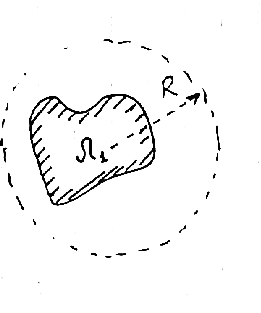
\includegraphics[scale = 0.4]{23_1_new}
\end{center}

Строим сферу радиуса $R \geqslant \widetilde{R}(\eps), \Omega_1 \subset B_R(o)$.
По следствию из принципа максимума $|v(x)|\leqslant~\max\limits_{\partial\Omega_1 \cup \partial B_R(0)} |v(y)|\leqslant ~\eps$

Т.к. $\eps > 0$ было выбрано произвольно, имеем $v(x) \equiv 0 \text{ в } \Omega \cup \text{Г}$
\end{proof}

\begin{theorem}
Не может существовать более 1 классического решения внешней задачи Неймана
\end{theorem}
\begin{proof}
Если $u_1,\  u_2$ - классические решения, то $\underbrace{v(x) = u_1 - u_2}_{\text{гармоническая в }\Omega\text{ и }C^2(\Omega)\cap C^2(\Omega \cup \text{Г})}$ -удовлетворяет полностью однородной задаче 
\[
\begin{cases}
\cfrac{\partial v}{\partial \bar{\vec n}}|_{\text{Г}} = 0\\
v(x) \rightarrow_{|x|\rightarrow \infty} 0 \ (\forall \eps > 0 \exists \widetilde{R}(\eps) : \forall x : |x| > \widetilde{R}(\eps) \rightarrow |v(x)|<\eps)
\end{cases}
\]
\begin{center}
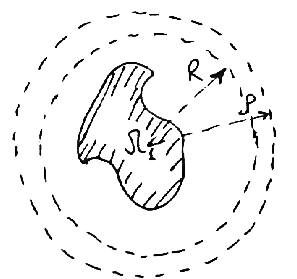
\includegraphics[scale = 0.4]{23_2_new}
\end{center}

Возьмем $R:\ \Omega_1 \subset B_R(0),\ \rho > R$. По I-ф-лу Грина для v
\[
\cancelto{0}{\int\limits_{B_R(0) \backslash \Omega_1} \Delta v \cdot v \cdot dx} = 
\cancelto{0}{\oint\limits_{\text{Г}} \cfrac{\partial v}{\partial \bar{\vec n}} v(x) dS_x} + \oint\limits_{\partial B_R(0)} \cfrac{\partial v}{\partial \bar{\vec n}} v(x) dS_x - \int\limits_{B_R(0) \backslash \Omega_1} |\nabla v(x)|^2 dx
\]

Получили $\int\limits_{B_R(0) \backslash \Omega_1} |\nabla v(x)|^2 dx = \oint\limits_{\partial B_R(0)} \cfrac{\partial v}{\partial \bar{\vec n}} v(x) dS_x$. Далее $\int\limits_{B_R(0) \backslash \Omega_1} |\nabla v(x)|^2 dx \leqslant \int\limits_{B_\rho(0) \backslash \Omega_1} |\nabla v(x)|^2 dx = \oint\limits_{\partial B_\rho(0)} \bigl|\cfrac{\partial v}{\partial \bar{\vec n}}\bigr| |v(x)| dS_x \leqslant (\text{ теорема об асимптотике гармонических функций }) \leqslant \cfrac{C_1}{\rho^2}\cdot \cfrac{C_2}{\rho}\cdot 4\pi\rho^2 \rightarrow 0 \text{ при }\rho \rightarrow \infty$.

Итак, $\nabla v(x) \equiv 0 \Rightarrow v(x) \equiv const = 0$, ч.т.д.
\end{proof}
\newpage
\section{Билет 24. Интегральные операторы с непрерывными и полярными ядрами в ограниченной области, их непрерывность в пространстве $C(\bar G)$. Приближение операторов с полярными ядрами операторами с непрерывными ядрами.}
% Затехал: Игорь Молибог
 
\begin{definition}[Интегральное уравнение Фредгольма второго рода]
Уравнение вида $$u(x) = \lambda \int_{G}K(x,y)u(y)dy + f(x)$$ называется интегральным уравнением Фредгольма 2-го рода.

Здесь:
\begin{itemize}
\item $x \in \bar G$, $G$ --- ограниченная область в $\R^3$;
\item $f(x) \in C(\bar G)$ --- задана;
\item $K(x, y): (\bar G \times \bar G) \to \R$.
\item $\lambda$ --- числовой параметр;
\item $u(x) \in C(\bar G)$ --- искомая функция.
\end{itemize} 
\end{definition}

\begin{definition}[Интегральный оператор]
Оператор $K$ такой, что $$(Ku)(x) = \int_{G}K(x,y)u(y)dy,$$ называется интегральным оператором с ядром $K(x,y).$
\end{definition}

\begin{theorem}
Если ядро $K(x,y) \in C(\bar G \times \bar G),$ то оператор $K$ ограничен в $C(\bar G)$ и имеет место оценка $$\|K\| \le \max_{x\in G}\int_G|K(x,y)|dy \le \max_{x,y \in \bar G}|K(x,y)|mes G$$

\end{theorem}

\begin{proof}

Если $K(x,y)\in C(\bar G \times \bar G),$ то $K:C(G) \to C(G)$.

$\|Ku\|_{C(\bar G)} = \max\limits_{\bar G} |(Ku)(x)| = \max\limits_{\bar G} |\int_G K(x,y)u(y)dy| \le  \max\limits_{\bar G} \int_G |K(x,y)||u(y)|dy \le \max_{x \in \bar G} \max\limits_{y \in \bar G} |u(y)|\int_G|K(x,y)|dy = \|u\|_{C(\bar G)}\max\limits_{x \in \bar G}\int_G|K(x,y)|dy \Rightarrow \|K\| = \sup\limits_{\|u\|_{C(\bar G)}=1}\frac{\|Ku\|_{C(\bar G)}}{\|u\|_{C(\bar G)}} \le \max_{x \in \bar G}\int_G |K(x,y)|dy$

\end{proof}


\begin{definition}[Полярное ядро]
Ядро $K(x,y)$ называется полярным, если его можно представить в виде $K(x,y) = \frac{\kappa(x,y)}{|x-y|^\alpha} \Forall x,y \in \bar G,\ x\ne y,$ где $\kappa \in C(\bar G \times \bar G),$ $\alpha < n$ --- размерность пространства.
\end{definition}

\begin{lemma}[Признак полярного ядра]
Ядро $K$ является полярным $\Leftrightarrow K(x,y) \in C((\bar G \times \bar G)\backslash\{x=y\})$ и $|K(x,y)| \le \frac{B}{|x-y|^\beta} \Forall x, y \in \bar G, x \ne y, B>0, \beta < n.$
\end{lemma}

\begin{proof}
($\Rightarrow$): Пусть ядро полярное. Тогда $\exists B: |\kappa| \le B$ на $\bar G \times \bar G$ и $|K| \le \frac{B}{|x-y|^\alpha}.$
\\
($\Leftarrow$): Пусть $\beta < n \Rightarrow \exists \eps > 0: \beta+\eps < n.$ Рассмотрим $\kappa =  \begin{cases}
   K(x,y)|x-y|^{\beta+\eps}, &x,y\in G, x\ne y;\\
   0, & x=y\in G.
 \end{cases}
$

Построенная $\kappa$ непрерывна в $(\bar G \times \bar G)\backslash\{x=y\}.$

Возьмем $x^0,y^0 \in G, x^0 \ne y^0:$
$|\kappa(x,y) - \kappa(x^0, x^0)| = |\kappa(x,y)| \le |K||x-y|^{\beta+\eps} \le \frac{B}{|x-y|^\beta}|x-y|^{\beta+\eps}\le B|x-y|^\eps = B|(x-x^0)-(y-y^0)|^\eps \le B(|x-x^0|+|y-y^0|)^\eps \Rightarrow \kappa$ непрерывна всюду в $\bar G \times \bar G.$

Очевидно из определения $\kappa,$ что можем записать $K(x,y) = \frac{\kappa(x,y)}{|x-y|^{\beta+\eps}},$ т.е. это ядро -- полярное по определению.
\end{proof}


\begin{definition}[Транспонированное ядро]
Ядром, транспонированным к ядру $K(x,y),$ называется ядро $K'(x,y) = K(y,x).$ Соответствующий оператор $K'$ так же называют транспонированным.
\end{definition}

\begin{theorem}
Интегральный оператор $K$ с полярным ядром является ограниченным оператором в $C(\bar G).$ Справедлива оценка: $\|K\| \le \sup_{x\in G}\int_G|K(x,y)|dy.$ $\Forall \eps > 0$ оператор $K$ можно представить в виде суммы $K = K_\eps^{cont}+K_\eps^{pol},$ где $\|K_\eps^{pol}\| \le \eps,$ $\|(K_\eps^{pol})'\| \le \eps,$ $K_\eps^{cont}$ --- и.о. с непрерывным ядром, $K_\eps^{pol}$ --- и.о. с полярным ядром.
\end{theorem}

\begin{proof} $\ $
\begin{enumerate}
\item{
Пусть $\psi(y) = K(x,y)u(y).$ Функция $\psi$ непрерывна при $y \ne x.$

В особенности: $|\psi(y)| = |K(x,y)||u(y)| \le \frac{B}{|x-y|^\alpha} \|u\|_{C(\bar G)}$ -- интегрируема, т.к. $\alpha < n.$

Значит, порождается функция $\phi(x) = \int_G\psi(y)dy = \int_G K(x,y)u(y)dy$ --- этот интеграл существует $\forall x \in \bar G.$
}

\item{Определим $\delta-$срезку функции $\frac{1}{|x-y|^\alpha}:$ $$\left(\frac{1}{|x-y|^\alpha}\right)_\delta = \begin{cases}
   \frac{1}{|x-y|^\alpha}, &|x-y|\ge \delta;\\
   \frac{1}{\delta^\alpha}, & |x-y|<\delta.
 \end{cases} \in C (\R^n \times \R^n)$$
}
\begin{center}
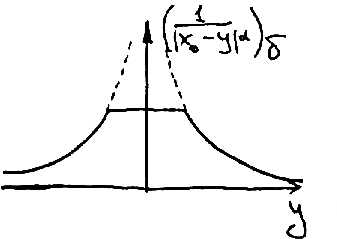
\includegraphics[width=0.2\textwidth]{24_1_new}
\end{center}

\item{Представим $K(x,y) = K^1_\delta (x,y) + K^2_\delta(x,y),$ где $K^1_\delta (x,y) = \kappa(x,y)(\frac{1}{|x-y|^\alpha})_\delta,$ $$K^2_\delta(x,y) = \begin{cases}
   0, &|x-y|\ge \delta;\\
   \kappa(x,y)(\frac{1}{|x-y|^\alpha}-\frac{1}{\delta^\alpha}), & |x-y|<\delta.
 \end{cases}$$
}

\item{ Выберем произвольно $u(x) \in C(\bar G)$ и рассмотрим $\|K^2_\delta u\|_{C(\bar G)}$: 

$\|K^2_\delta u\| = \max_{x \in G} |\int_{|y-x|<\delta}\kappa(x,y)(\frac{1}{|x-y|^\alpha}-\frac{1}{\delta^\alpha})u(y)dy| \le B\|u\|_{C(\bar G)}\int_{|y-x|<\delta}\frac{dy}{|x-y|^\alpha} = B \|u\|_{C(\bar G)}\int_{|z|<\delta}\frac{dz}{|z|^\alpha}.
$

Замена $\begin{cases}
   x_k = r\sin\phi_1...\sin\phi_{k-1}\cos\phi_k, &k = 1, \dots, n-1;\\
   x_n = r\sin\phi_1...\sin\phi_{n-1},
 \end{cases}$ где $\phi_k \in [0, \Pi], \phi_n \in [0, 2\Pi]$
 
Якобиан $J = \frac{D(x_1, \dots, x_n)}{D(r, \phi_1, \dots, \phi_{n-1})} = r^{n-1}\sin^{n-2}\phi_1\sin^{n-3}\phi_2\dots\sin\phi_{n-1}.$ Получили:

$$\|K^2_\delta a\| \le C_1\|u\|_{C(G)}\int_0^\delta\frac{r^{n-1}}{r^\alpha}dr = C\|u\|_{C(G)}\delta^{n-\alpha} \to 0 \text{ при } \delta \to 0.$$

Получили $K^2_\delta u \to Ku$ по норме $\Rightarrow Ku \in C(\bar G).$
 
}

\item{$\|K\| \le \|K^1_\delta\| + \|K^2_\delta\|\le C\delta^{n-\alpha} + \|K^1_\delta\| < \infty$ $\Rightarrow K$ --- ограничен.

Для транспонированного ядра все рассуждения аналогичны, т.к. полярное ядро $K = \frac{\kappa(x,y)}{|x-y|^\alpha}$ при замене $x$ на $y$ изменяет только непрерывный числитель $\kappa$.
}

\end{enumerate}
\end{proof}











\newpage
\section{Билет 25. Интегральное уравнение Фредгольма второго рода с малым по норме интегральным оператором $K$. Представление решения рядом Неймана. Ограниченность оператора $(I-\lambda K)^{-1}.$}
% Затехал: Багно Богдан
Рассмотрим уравнение
$$u(x) = \lambda \int_{G}K(x,y)u(y)dy + f(x), \; x \in \overline{G} \eqno(1)$$
\begin{theorem}
Пусть в интегральном уравнении (1) ядро K полярное и выполнено $\abs{\lambda}\cdot\norm{K} < 1$, тогда:
  \begin{itemize}
    \item $\forall f \in C(G)$ (1) имеет единственное решение $u(x) \in C(\overline{G})$.  Это решение при фиксированном $\lambda_{fix}$ представимо абсолютно сходящимся в $C(\overline{G})$ рядом Неймана:
    $$u(x) = f(x) + \sum_{i=1}^{\infty}\lambda^{i}K^{i}f(x),\; x \in G$$
    \item Оператор $I - \lambda K$ отображает всё $C(\overline{G})$ на всё $C(\overline{G})$ и имеет на $C(\overline{G})$ непрерывный обратный оператор $(I - \lambda K)^{-1}$, причём $\norm{(I - \lambda K)^{-1}} \leq (1 - \abs{\lambda}\cdot\norm{K})^{-1}$
  \end{itemize}
\end{theorem}

\begin{proof}
  \begin{enumerate} 
  	\item Отметим, что оператор $\lambda K$ сжимающий: $\norm{\lambda K} = \abs{\lambda}\cdot\norm{K} < 1$. \\Построим итерационный процесс:
    $$u_{0} = f(x)$$
    $$u_{1} = f(x) + \lambda K u_{0}(x) = f(x) + \lambda K f(x)$$
    $$\cdots$$
    $$u_{n} = f(x) + \sum_{i=1}^{n}\lambda^{i}K^{i}f(x)$$
    $$\cdots$$
    Все $u_{k}(x) \in C(\overline{G})$, причем $u_{k} = S_{k}$ -- k-я частичная сумма ряда Неймана.
    Далее, $$\norm{\lambda^{i}K^{i}f(x)}_{C(\overline{G})} \leq \abs{\lambda^{i}}\cdot\norm{K}^{i}\cdot\norm{f}_{C(\overline{G})}=(\abs{\lambda}\cdot\norm{K})^{i}\norm{f}_{C(\overline{G})}\Longrightarrow$$ 
    $$\Longrightarrow \sum_{i=0}^{\infty}\norm{\lambda^{i}K^{i}f(x)}_{C(\overline{G})} \leq \sum_{i=0}^{\infty}(\abs{\lambda}\cdot\norm{K})^{i}\norm{f} = \frac{\norm{f}}{1 - \abs{\lambda}\cdot\norm{K}}.$$
    Указанный в условии ряд сходится абсолютно в банаховом пространстве $C(\overline{G})$ $\Longrightarrow$ он сходится $\Longrightarrow$ \\ $\Longrightarrow \exists u(x) \in C(\overline{G}): \norm{U - U_{n}}_{C(\overline{G})} \xrightarrow[n \longrightarrow \infty]{} 0 \Longrightarrow U_{n} \xrightarrow{\norm{\cdot}_{C(\overline{G})}} U$
    \begin{itemize}
	  \item Покажем что U -- решение: $U_{n} = f + \lambda K U_{n-1}$, при этом $U_{n} \longrightarrow U$ а $\lambda K U_{n-1} \longrightarrow \lambda K U$ в силу непрерывности оператора $K$.
      \item Единственность: пусть $U_{I}$, $U_{II}$ -- решения, обозначим $V = U_{I} - U_{II} \in \overline{G}$. При этом $V$ удовлетворяет однородному уравнению $V = \lambda K V, \; x \in C(\overline{G})$. Тогда $$\|V\| \leq \abs{\lambda}\cdot\norm{K}\cdot\norm{V} \longrightarrow (1 - \abs{\lambda}\cdot\norm{K})\cdot\norm{V} \leq 0 \longrightarrow \norm{V} = 0 \longrightarrow V \equiv 0$$
	\end{itemize}
    \item $u = \lambda Ku + f \longleftrightarrow (I - \lambda  K)u = f$. То, что $I - \lambda K$ отображает всё $C(\overline{G}),$ -- ясно. Согласно пункту 1 $\forall f \in C(\overline{G}) \exists ! u(x)$ -- решение, значит оператор отображает всё $C(\overline{G})$ на всё $C(\overline{G})$. Значит, существует обратный оператор $(I - \lambda K)^{-1}$. Он ограничен т.к. $$\norm{(I - \lambda K)^{-1}f}_{C(\overline{G})} = \norm{U}_{C(\overline{G})} \leq \sum_{i = 0}^{\infty}\norm{\lambda^{i}K^{i}f}_{C(\overline{G})} \leq \frac{\norm{f}_{C(\overline{G})}}{1 - \abs{\lambda}\cdot\norm{K}} < \infty$$
  \end{enumerate}
\end{proof}

\newpage

\section{Интегральное уравнение Фредгольма второго рода с малым по норме интегральным оператором $\lambda K$. Представление решения интегрального уравнения рядом Неймана. Ограниченность оператора $(I-\lambda K)^{-1}.$}
% Затехал: Багно Богдан

\begin{definition}[Интегральное уравнение Фредгольма второго рода]
Уравнение вида $$u(x) = \lambda \int_{G} \mathcal{K}(x,y)u(y)dy + f(x)$$ называется интегральным уравнением Фредгольма 2-го рода.

Здесь:
\begin{itemize}
\item $x \in \overline{G}$, $G$ -- ограниченная область в $\R^3$;
\item $f(x) \in C(\overline{G})$ -- задана;
\item $ \mathcal{K}(x, y): \overline{G} \times \overline{G} \to \R$;
\item $\lambda$ -- числовой параметр;
\item $u(x) \in C(\overline{G})$ -- искомая функция.
\end{itemize} 
\end{definition}

\begin{definition}[Интегральный оператор]
Оператор $K$ такой, что $$(Ku)(x) = \int_{G} \mathcal{K}(x,y)u(y)dy,$$ называется интегральным оператором с ядром $ \mathcal{K}(x,y).$
\end{definition}

\begin{theorem}
Если ядро $ \mathcal{K}(x,y) \in C(\overline{G} \times \overline{G}),$ то оператор $K$ ограничен в $C(\overline{G})$ и имеет место оценка $$\|K\| \le \max_{x \in G}\int_G |\mathcal{K}(x,y)|dy \le \max_{x,y \in \overline{G}} |\mathcal{K}(x,y)| \cdot mes (G)$$

\end{theorem}

\begin{proof}

Если $\mathcal{K}(x,y)\in C(\overline{G} \times \overline{G}),$ то $K:C(G) \to C(G)$.

$\|Ku\|_{C(\overline{G})} = \max\limits_{x \in \overline{G}} |(Ku)(x)| = \max\limits_{x \in \overline{G}} |\int_G \mathcal{K}(x,y)u(y)dy| \le  \max\limits_{x \in \overline{G}} \int_G |\mathcal{K}(x,y)||u(y)|dy \le \max\limits_{x \in \overline{G}} \max\limits_{y \in \overline{G}} |u(y)|\int_G|\mathcal{K}(x,y)|dy = \|u\|_{C(\overline{G})}\max\limits_{x \in \overline{G}}\int_G|\mathcal{K}(x,y)|dy \Rightarrow \|K\| = \sup\limits_{\|u\|_{C(\overline{G})}=1}\frac{\|Ku\|_{C(\overline{G})}}{\|u\|_{C(\overline{G})}} \le \max\limits_{x \in \overline{G}}\int_G |\mathcal{K}(x,y)|dy$

\end{proof}


\begin{definition}[Полярное ядро]
Ядро $\mathcal{K}(x,y)$ называется полярным, если его можно представить в виде $\mathcal{K}(x,y) = \frac{\kappa(x,y)}{|x-y|^\alpha} \Forall x,y \in \overline{G},\ x\ne y,$ где $\kappa \in C(\overline{G} \times \overline{G}),$ $\alpha < n$ -- размерность пространства.
\end{definition}

\begin{lemma}[Признак полярного ядра]
Ядро $\mathcal{K}$ является полярным $\Leftrightarrow \mathcal{K}(x,y) \in C((\overline{G} \times \overline{G})\backslash\{x=y\})$ и $|\mathcal{K}(x,y)| \le \frac{B}{|x-y|^\beta} \, \Forall x, y \in \overline{G}, \, x \ne y, \, B>0, \, \beta < n.$
\end{lemma}

\begin{proof}
($\Rightarrow$): Пусть ядро полярное. Тогда $\exists B: |\kappa| \le B$ на $\overline{G} \times \overline{G}$ и $|\mathcal{K}| \le \frac{B}{|x-y|^\alpha}.$
\\
($\Leftarrow$): Пусть $\beta < n \Rightarrow \Exists \eps > 0: \beta+\eps < n.$ Рассмотрим $\kappa =  \begin{cases}
   \mathcal{K}(x,y)|x-y|^{\beta+\eps}, &x,y\in G, x\ne y;\\
   0, & x=y\in G.
 \end{cases}
$

Построенная $\kappa$ непрерывна в $(\overline{G} \times \overline{G})\backslash\{x=y\}.$

Возьмем $x^0,y^0 \in G, x^0 \ne y^0:$
$|\kappa(x,y) - \kappa(x^0, x^0)| = |\kappa(x,y)| \le |\mathcal{K}||x-y|^{\beta+\eps} \le \frac{B}{|x-y|^\beta}|x-y|^{\beta+\eps}\le B|x-y|^\eps = B|(x-x^0)-(y-y^0)|^\eps \le B(|x-x^0|+|y-y^0|)^\eps \Rightarrow \kappa$ непрерывна всюду в $\overline{G} \times \overline{G}.$

Очевидно из определения $\kappa,$ что можем записать $\mathcal{K}(x,y) = \frac{\kappa(x,y)}{|x-y|^{\beta+\eps}},$ т.е. это ядро -- полярное по определению.
\end{proof}


\begin{definition}[Транспонированное ядро]
Ядром, транспонированным к ядру $\mathcal{K}(x,y),$ называется ядро $\mathcal{K}'(x,y) = \mathcal{K}(y,x).$ Соответствующий оператор $K'$ так же называют транспонированным.
\end{definition}

\begin{theorem}
Интегральный оператор $K$ с полярным ядром является ограниченным оператором в $C(\overline{G}).$ Справедлива оценка: $\|K\| \le \sup_{x\in G}\int_G|\mathcal{K}(x,y)|dy.$ $\Forall \eps > 0$ оператор $K$ можно представить в виде суммы $K = K_\eps^{cont}+K_\eps^{pol},$ где $\|K_\eps^{pol}\| \le \eps,$ $\|(K_\eps^{pol})'\| \le \eps,$ $K_\eps^{cont}$ -- и.о. с непрерывным ядром, $K_\eps^{pol}$ -- и.о. с полярным ядром.
\end{theorem}

\begin{proof} $\ $
\begin{enumerate}
\item{
Пусть $\psi(y) = \mathcal{K}(x,y)u(y).$ Функция $\psi$ непрерывна при $y \ne x.$

В особенности: $|\psi(y)| = |\mathcal{K}(x,y)||u(y)| \le \frac{B}{|x-y|^\alpha} \|u\|_{C(\overline{G})}$ -- интегрируема, т.к. $\alpha < n.$

Значит, порождается функция $\phi(x) = \int_G\psi(y)dy = \int_G \mathcal{K}(x,y)u(y)dy$ -- этот интеграл существует $\forall x \in \overline{G}.$
}

\item{Определим $\delta-$срезку функции $\frac{1}{|x-y|^\alpha}:$ $$\left(\frac{1}{|x-y|^\alpha}\right)_\delta = \begin{cases}
   \frac{1}{|x-y|^\alpha}, &|x-y|\ge \delta;\\
   \frac{1}{\delta^\alpha}, & |x-y|<\delta.
 \end{cases} \in C (\R^n \times \R^n)$$
}
\begin{center}
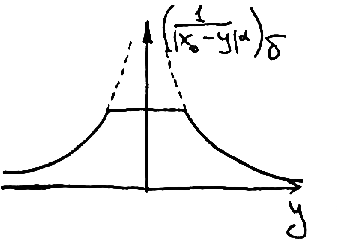
\includegraphics[width=0.2\textwidth]{26_1_new}
\end{center}

\item{Представим $\mathcal{K}(x,y) = \mathcal{K}^1_\delta (x,y) + \mathcal{K}^2_\delta(x,y),$ где $\mathcal{K}^1_\delta (x,y) = \kappa(x,y)(\frac{1}{|x-y|^\alpha})_\delta,$ $$\mathcal{K}^2_\delta(x,y) = \begin{cases}
   0, &|x-y|\ge \delta;\\
   \kappa(x,y)(\frac{1}{|x-y|^\alpha}-\frac{1}{\delta^\alpha}), & |x-y|<\delta.
 \end{cases}$$
}

\item{ Выберем произвольно $u(x) \in C(\overline{G})$ и рассмотрим $\|K^2_\delta u\|_{C(\overline{G})}$: 

$\|K^2_\delta u\| = \max\limits_{x \in G} |\int_{|y-x|<\delta}\kappa(x,y)(\frac{1}{|x-y|^\alpha}-\frac{1}{\delta^\alpha})u(y)dy| \le B\|u\|_{C(\overline{G})}\int_{|y-x|<\delta}\frac{dy}{|x-y|^\alpha} = B \|u\|_{C(\overline{G})}\int_{|z|<\delta}\frac{dz}{|z|^\alpha}.
$

Замена $\begin{cases}
   x_k = r\sin\phi_1...\sin\phi_{k-1}\cos\phi_k, &k = 1, \dots, n-1;\\
   x_n = r\sin\phi_1...\sin\phi_{n-1},
 \end{cases}$ где $\phi_k \in [0, \Pi], \phi_n \in [0, 2\Pi]$
 
Якобиан $J = \frac{D(x_1, \dots, x_n)}{D(r, \phi_1, \dots, \phi_{n-1})} = r^{n-1}\sin^{n-2}\phi_1\sin^{n-3}\phi_2\dots\sin\phi_{n-1}.$ Получили:

$$\|K^2_\delta a\| \le C_1\|u\|_{C(G)}\int_0^\delta\frac{r^{n-1}}{r^\alpha}dr = C\|u\|_{C(G)}\delta^{n-\alpha} \to 0 \text{ при } \delta \to 0.$$

Получили $K^2_\delta u \to Ku$ по норме $\Rightarrow Ku \in C(\overline{G}).$
 
}

\item{$\|K\| \le \|K^1_\delta\| + \|K^2_\delta\|\le C\delta^{n-\alpha} + \|K^1_\delta\| < \infty$ $\Rightarrow K$ -- ограничен.

Для транспонированного ядра все рассуждения аналогичны, т.к. полярное ядро $K = \frac{\kappa(x,y)}{|x-y|^\alpha}$ при замене $x$ на $y$ изменяет только непрерывный числитель $\kappa$.
}

\end{enumerate}
\end{proof}





Рассмотрим уравнение
$$u(x) = \lambda \int_{G}\mathcal{K}(x,y)u(y)dy + f(x), \; x \in \overline{G} \eqno(1)$$
\begin{theorem}
Пусть в интегральном уравнении (1) ядро $\mathcal{K}$ полярное и выполнено $\abs*{\lambda}\cdot\norm*{K} < 1$, тогда:
  \begin{itemize}
    \item $\forall f \in C(\overline{G})$ (1) имеет единственное решение $u(x) \in C(\overline{G})$.  Это решение при фиксированном $\lambda_{\mathrm{fix}}$ представимо абсолютно сходящимся в $C(\overline{G})$ рядом Неймана:
    $$u(x) = f(x) + \sum_{i=1}^{\infty}\lambda^{i}K^{i}f(x),\; x \in G$$
    \item Оператор $I - \lambda K$ отображает всё $C(\overline{G})$ на всё $C(\overline{G})$ и имеет на $C(\overline{G})$ непрерывный обратный оператор $(I - \lambda K)^{-1}$, причём $\norm*{(I - \lambda K)^{-1}} \leq (1 - \abs*{\lambda}\cdot\norm*{K})^{-1}$
  \end{itemize}
\end{theorem}

\begin{proof}
  \begin{enumerate} 
  	\item Отметим, что оператор $\lambda K$ сжимающий: $\norm*{\lambda K} = \abs*{\lambda}\cdot\norm*{K} < 1$. \\Построим итерационный процесс:
    $$u_{0} = f(x)$$
    $$u_{1} = f(x) + \lambda K u_{0}(x) = f(x) + \lambda K f(x)$$
    $$\cdots$$
    $$u_{n} = f(x) + \sum_{i=1}^{n}\lambda^{i}K^{i}f(x)$$
    $$\cdots$$
    Все $u_{k}(x) \in C(\overline{G})$, причем $u_{k} = S_{k}$ -- k-я частичная сумма ряда Неймана.
    Далее, $$\norm*{\lambda^{i}K^{i}f(x)}_{C(\overline{G})} \leq \abs*{\lambda^{i}}\cdot\norm*{K}^{i}\cdot\norm*{f}_{C(\overline{G})}=(\abs*{\lambda}\cdot\norm*{K})^{i}\norm*{f}_{C(\overline{G})}\Longrightarrow$$ 
    $$\Longrightarrow \sum_{i=0}^{\infty}\norm*{\lambda^{i}K^{i}f(x)}_{C(\overline{G})} \leq \sum_{i=0}^{\infty}(\abs*{\lambda}\cdot\norm*{K})^{i}\norm*{f} = \frac{\norm*{f}}{1 - \abs*{\lambda}\cdot\norm*{K}}.$$
    Указанный в условии ряд сходится абсолютно в банаховом пространстве $C(\overline{G})$ $\Longrightarrow$ он сходится $\Longrightarrow$ \\ $\Longrightarrow \Exists u(x) \in C(\overline{G}): \norm*{u - u_{n}}_{C(\overline{G})} \xrightarrow[n \longrightarrow \infty]{} 0 \Longrightarrow u_{n} \xrightarrow{\norm*{\cdot}_{C(\overline{G})}} u$
    \begin{itemize}
	  \item Покажем что $u$ -- решение: $u_{n} = f + \lambda K u_{n-1}$, при этом $u_{n} \longrightarrow u$ а $\lambda K u_{n-1} \longrightarrow \lambda K u$ в силу непрерывности оператора $K$.
      \item Единственность: пусть $u_{I}$, $u_{II}$ -- решения, обозначим $v = u_{I} - u_{II} \in \overline{G}$. При этом $v$ удовлетворяет однородному уравнению $v = \lambda K v, \; x \in C(\overline{G})$. Тогда $$\|v\| \leq \abs*{\lambda}\cdot\norm*{K}\cdot\norm*{v} \longrightarrow (1 - \abs*{\lambda}\cdot\norm*{K})\cdot\norm*{v} \leq 0 \longrightarrow \norm*{v} = 0 \longrightarrow v \equiv 0$$
	\end{itemize}
    \item $u = \lambda Ku + f \longleftrightarrow (I - \lambda  K)u = f$. То, что $I - \lambda K$ отображает всё $C(\overline{G}),$ -- ясно. Согласно пункту 1 $\forall f \in C(\overline{G}) \;\;\exists!\ u(x)$ -- решение, значит оператор отображает всё $C(\overline{G})$ на всё $C(\overline{G})$. Значит, существует обратный оператор $(I - \lambda K)^{-1}$. Он ограничен т.к. $$\norm*{(I - \lambda K)^{-1}f}_{C(\overline{G})} = \norm*{u}_{C(\overline{G})} \leq \sum_{i = 0}^{\infty}\norm*{\lambda^{i}K^{i}f}_{C(\overline{G})} \leq \frac{\norm*{f}_{C(\overline{G})}}{1 - \abs*{\lambda}\cdot\norm*{K}} < \infty$$
  \end{enumerate}
\end{proof}

\newpage
	\section{Интегральное уравнение Фредгольма второго рода с непрерывными и полярными ядрами. Теоремы Фредгольма. Дискретность множества характеристических чисел.}
% Затехал: Багно Богдан
Рассмотрим уравнение
$$u(x) = \lambda \int_{G}K(x,y)u(y)dy + f(x), \; x \in \overline{G} \eqno(1)$$
и ему союзное
$$v(x) = \lambda \int_{G}K'(x,y)v(y)dy + g(x), \; x \in \overline{G}, K'(x,y) = K(y,x) \eqno(2)$$

\begin{theorem}[Первая теорема Фредгольма (Теорема Фредгольма об альтернативах)]
  Либо интегральное уравнение (1) однозначно разрешимо в $C(\overline{G})$ для каждой функции $f(x)$ из $C(\overline{G})$ либо соответствующее однородное уравнение имеет по крайней мере одно нетривиальное решение.
\end{theorem}
\begin{theorem}[Вторая теорема Фредгольма]
  Если для уравнения (1) имеет место первый случай альтернативы, то он же имеет место и для уравнения (2). Как однородное уравнение соответствующее (1) так и однородное уравнение соответствующее (2) имеют конечные числа линейно независимых собственных функций, причем эти числа совпадают.
\end{theorem}
\begin{theorem}[Третья теорема Фредгольма]
  Если для уравнения (1) имеет место второй случай альтернативы, то неоднородное уравнение (1) разрешимо в $C(\overline{G})$ тогда и только тогда, когда выполнено условие "ортогональности":
   $$\int_{G}f(y)v(y)dy = 0$$
\end{theorem}
\begin{theorem}
  В любом круге $\abs*{\lambda} < R$ на $\C$ у ядра уравнения (1) имеется не более чем конечное количество характеристических чисел. Единственная возможная точка накопления характеристических чисел -- бесконечно удаленная точка.
\end{theorem}

Билет посвящен доказательству этих теорем.

\begin{theorem}[Апроксимационная теорема Вейерштрасса]
  Пусть $\Omega$ -- ограниченная область в $\R^{n}$, а $W(x) \in C(\overline{G})$. Тогда $\forall \varepsilon > 0 \Exists P_{\varepsilon}(x)$ -- многочлен от $x_{1}..x_{n}$ такой, что $\norm*{h(x) - P_{\varepsilon}(x)}_{C(\overline{G})} < \varepsilon$.
\end{theorem}

Будем использовать данный факт из анализа.

\begin{lemma}
  Пусть $K$ -- интегральный оператор с непрерывным ядром $K(x,y)$ $K(x,y) \in \brk[a]*{C(\overline{G});C(\overline{G})}$. Тогда $\forall \varepsilon > 0$ этот оператор можно представить в виде $K = \overset{B}{\Phi_{\varepsilon}} + \overset{H}{K_{\varepsilon}}, \; \norm*{\overset{H}{K_{\varepsilon}}} < \varepsilon, \; \norm*{\overset{H}{K_{\varepsilon}^{'}}} < \varepsilon$
\end{lemma}
\begin{proof}
  По $\varepsilon > 0$ найдем $P_{\varepsilon}(x,y)$ от $x_{1}..x_{n},y_{1}..y_{n} : \norm*{K(x,y) - P_{\varepsilon}(x,y)}_{C(\overline{G})} < \varepsilon$. Тогда $\norm*{\overset{H}{K_{\varepsilon}}} \leq \norm*{K(x,y) - P_{\varepsilon}(x,y)}_{C(\overline{G})}\cdot mes G = \varepsilon\cdot mes G$. При этом оператор $\overset{B}{\Phi_{\varepsilon}}$ имеет вырожденное ядро $P_{\varepsilon}$.
\end{proof}

\begin{lemma}
  Пусть $K$ -- интегральный оператор с полярным ядром $K(x,y)$ $K(x,y) \in \brk[a]*{C(\overline{G});C(\overline{G})}$. Тогда $\forall \varepsilon > 0$ этот оператор можно представить в виде $K = \overset{B}{\Phi_{\varepsilon}} + \overset{\Pi}{Q_{\varepsilon}}, \; \norm*{\overset{\Pi}{Q_{\varepsilon}}} < \varepsilon, \; \norm*{\overset{\Pi}{Q_{\varepsilon}^{'}}} < \varepsilon$
\end{lemma}
\begin{proof}
Представим $K$ в виде суммы $\overset{H}{K_{\varepsilon}} + \overset{\Pi}{K_{\frac{\varepsilon}{2}}}$. По предыдущей лемме $\overset{H}{K} = \Phi+ \overset{H}{K_{\frac{\varepsilon}{2}}}$. Значит, $K = \Phi+ \overset{H}{K_{\frac{\varepsilon}{2}}} + \overset{\Pi}{K_{\frac{\varepsilon}{2}}} = \Phi + \overset{\Pi}{Q_{\varepsilon}}, \; \norm*{\overset{\Pi}{Q_{\varepsilon}}} \leq \frac{\varepsilon}{2} + \frac{\varepsilon}{2} = \varepsilon$
\end{proof}

Перейдем к теоремам Фредгольма.

Пусть $R > 0, \overline{D_{R}} = \brk[c]*{\lambda \in \C: \abs*{\lambda} < R}$.

\begin{itemize}
  \item Возьмем $\varepsilon = \frac{1}{2R}, \; K = \Phi + Q, \; P = P(x,y)=\sum_{j = 1}^{N} a_{j}(x)b_{j}(y), \; \norm*{Q}, \norm*{Q^{'}} < \varepsilon$
  \item Представим уравнение $u = \lambda Ku +f$ в виде $(I -\lambda K)u = \lambda \Phi u + f$, аналогично, его союзное уравнение $v = \lambda K^{'}v +g$ представим в виде $(I -\lambda K^{'})v = \lambda \Phi^{'} v + g$. Далее представим эти уравнения в следующей форме:
  $$ (I - \lambda Q)u = \lambda \sum_{j = 1}^{N}a_{j}(x)\int_{G}b_{j}(y)u(y)dy + f(x)$$
  $$ (I - \lambda Q^{'})v = \lambda \sum_{j = 1}^{N}b_{j}(x)\int_{G}a_{j}(y)v(y)dy + g(x)$$
  \item $Q$ -- оператор с малой нормой: $\abs*{\lambda}\cdot\norm*{Q} \leq \frac{\abs*{\lambda}}{2R} < 1$. Аналогичные рассуждения верны и для оператора $Q^{'}$, а значит операторы $(I - \lambda Q), (I - \lambda Q^{'})$ непрерывно обратимы. Перепишем уравнения:
  $$u(x) = \lambda \sum_{j = 1}^{N}\underbrace{(I - \lambda Q)^{-1}a(x)}_{\hat{a}_{j}(x,\lambda)}\int_{G}b_{j}(y)u(y)dy + \underbrace{(I - \lambda Q)^{-1}f(x)}_{\hat{f}(x)} = \lambda \sum_{j = 1}^{N}\hat{a}_{j}(x,\lambda)\int_{G}b_{j}(y)u(y)dy + \hat{f}(x,\lambda)$$
  $$v(x) = ... = \lambda \sum_{j = 1}^{N}\hat{b}_{j}(x,\lambda)\int_{G}a_{j}(y)u(y)dy + \hat{g}(x,\lambda)$$
  
  Это уравнения с вырожденными ядрами, их решение эквивалентно решению систем:
  $$(E - \lambda \hat{A})\vec{c} = \vec{\varphi}; \; \hat{A}(\lambda) = \norm*{\mu_{ij}}_{i,j=1}^{N}; \; \mu_{i,j} = \brk[a]*{b_{i}; \hat{a}_{j}}; \; \varphi_{i} = \brk[a]*{b_{i}; \hat{f}}$$
  $$(E - \lambda \hat{A^{'}})\vec{d} = \vec{\phi}; \; \hat{A}^{'}(\lambda) = \norm*{\mu^{'}_{ij}}_{i,j=1}^{N}; \; \mu^{'}_{i,j} = \brk[a]*{a_{i}; \hat{b}_{j}}; \; \phi_{i} = \brk[a]*{a_{i}; \hat{g}}$$
  
  \begin{lemma}
    Пусть $K$ -- полярное ядро такое, что $\norm*{\lambda K} < 1$. Тогда $\forall a, b \in C(\overline{G}) \longrightarrow \brk[a]*{(I - \lambda K)^{-1}a; b} = \int_{G}(I - \lambda K)^{-1}a(x)b(x)dx$ -- регулярная функция при $\abs*{\lambda} < \norm*{K}^{-1}$. Если дополнительно выполнено $\abs*{\lambda}\cdot\norm*{K^{'}} < 1$, то $\brk[s]*{(I - \lambda K)^{-1}a; b} = \brk[s]*{a; (I - \lambda K^{'})^{-1}b}$.
  \end{lemma}
  \begin{proof}
    $$ (I - \lambda K)^{-1}a(x) = \sum_{j = 0}^{\infty}\lambda^{j}K^{j}a(x) \Longrightarrow \int_{G}(I - \lambda K)^{-1}a(x)b(x)dx = \int_{G} \underbrace{\sum_{j = 0}^{\infty}\lambda^{j}K^{j}(a(x))b(x)}_{\text{сход. равномерно}}dx = \sum_{j = 0}^{\infty}\lambda^{j}\brk[s]*{\int_{G}K^{j}(a(x))b(x)dx}$$
    Полученный ряд сходится абсолютно т.к. справедлива оценка
    $$ \abs*{\lambda^{j}\int_{G}K^{j}(a(x))b(x)dx} \leq \norm*{a}\cdot\norm*{b}\cdot mes G \cdot \underbrace{\abs*{\lambda^{j}\cdot\norm*{K}^{j}}}_{q_{j}; \; q < 1}$$
    Докажем теперь вторую часть:
     $$\norm*{\lambda K^{'}} < 1 \Longrightarrow \Exists (I - \lambda K^{'})^{-1} \in \mathcal{L}(C(\overline{G})) \Longrightarrow (I - \lambda K^{'})^{-1}b = \sum_{j = 0}^{inf}\lambda^{j}(K^{'})^{j}b(x)$$
     Тогда:
     $$\brk[a]*{(I - \lambda K)^{-1}a; b} \overset{*}{=} \sum_{j=0}^{\infty}\lambda^{j}\brk[a]*{K^{j}a; b} = \sum_{j=0}^{\infty}\lambda^{j}\brk[a]*{a; (K^{'})^{j}b} = \brk[a]*{a; \sum_{j=0}^{\infty}\lambda^{j}(K^{'})^{j}b} = \brk[a]*{a; (I - \lambda K^{'})^{-1}b}$$
      Докажем (*):
     $$ \brk[a]*{Ku; v} = \int_{G}\int{G}K(x,y)u(y)dyv(x)dx =$$
     $$=  \int_{G}u(y)\brk[s]*{\int{G}K(x,y)v(x)d(x)}dy = \brk[s]*{x \rightarrow y; y \rightarrow x; (**)} =$$
     $$= \int_{G}u(x)\brk[s]*{\int{G}\underbrace{K(y,x)}_{K^{'}(x,y)}v(y)dy}dx = \brk[a]*{u; K^{'}v}$$
     Где переход (**) верен по т. Фубини-Тонелли.
  \end{proof}
  \begin{lemma}
    Матрица $\hat{A}^{'}(\lambda)$ является транспонированной к матрице $\hat{A}(\lambda)$. Элементы $\hat{mu}_{ij}$ матрицы $\hat{A}$ -- регулярные в круге $\abs*{\lambda} < 2R$ функции $\lambda$.
  \end{lemma}
  \begin{proof}
    $$\abs*{\lambda} < 2R \Longrightarrow \abs*{\lambda}\cdot\norm*{Q} < 1, \; \abs*{\lambda}\cdot\norm*{Q^{'}} < 1$$
    $$\hat{\mu}^{'}_{ij} = \brk[a]*{a_{i}; (I - \lambda Q^{'})^{-1}b_{j}} = \brk[a]*{(I - \lambda Q)^{-1}a_{i}; b_{j}} = \hat{\mu}_{ji}$$
    Регулярность следует из предыдущей леммы.
  \end{proof}
  \item Рассмотрим $D(\lambda) = det(E - \lambda\hat{A}(\lambda)) = det(E - \lambda\hat{A}^{'}(\lambda))$. Это регулярная в круге $\abs*{\lambda} < 2R$ функция, $D(0) = 1 \Longrightarrow D(\lambda) \not \equiv 0$.
  
  В круге $\abs*{\lambda} < R$ может быть только конечное число нулей $\lambda_{k}$ иначе по теореме о единственности имели бы $D(\lambda) \equiv 0$.
  
  Если $\lambda$ не корень $D(\lambda) = 0$ то оба уравнения однозначно разрешимы.
  
  Если же $\lambda$ -- корень $D(\lambda) = 0$, то оба уравнения имеют конечномерные пространства решений одной размерности.
  
  Таким образом, мы доказали следующие эквивалентности:
  \begin{itemize}
    \item разрешимость исходного уравнения
    \item разрешимость системы
    $$u(x) = \lambda \sum_{j = 1}^{N}\hat{a}_{j}(x,\lambda)\int_{G}b_{j}(y)u(y)dy + \hat{f}(x,\lambda)$$
    \item разрешимость $(E - \lambda \hat{A^{'}})\vec{d} = \vec{\phi}$
  \end{itemize}
\end{itemize}
  
  Осталась третья теорема: условие разрешимости: $\vec{\varphi} \perp \vec{d}_{\text{одн}}$ -- любому решению $\brk[s]*{E - \lambda\hat{A}^{'}(\lambda)} = \vec{0}$ т.е.
  $$ \underbrace{\sum_{j=1}^{N}\hat{\varphi}d_{j}}_{0} = \sum_{j=1}^{N}\brk[a]*{b_{j}; \hat{f}}d_{j} = \sum_{j=1}^{N}\brk[a]*{b_{j}; (I - \lambda Q)^{-1}f}_{j}=$$
  $$= \sum_{j=1}^{N}\brk[a]*{f; (I - \lambda Q^{'})^{-1}b_{j}}_{j} = \brk[a]*{f, \sum_{j=1}^{N}\underbrace{(I - \lambda Q^{'})^{-1}b_{j}}_{\hat{b_{j}}}d_{j}} = \brk[a]*{f; v} = \int_{G}fvdx = 0$$
\newpage
\section{Билет 28. Объемный ньютонов потенциал и его свойства. Убывание на бесконечности. Результат
действия оператора Лапласа на объемный потенциал.}

\begin{itemize}
	\item Функция $E(x) = \frac{-1}{4\pi|x|}$ является решением в обобщенных функциях уравнения $\triangle E(x) = \delta (x)$. Эту запись нужно понимать следующим образом:
    $$
    \int\limits_{\mathbb{R}^3}\brs{\frac{-1}{4\pi|y|}}\Delta_y \varphi (y) \mathrm{d}y = \varphi(0),\; \varphi \in D(\mathbb{R}^n)
    $$
\end{itemize}

\begin{definition}
	Функция $\vartheta (x)$ вида $\vartheta (x) = \int\limits_{\mathbb{R}^3}\frac{\rho (y)}{|x-y|}\mathrm{d}y$ называется \underline{\it \text{объемным ньютоновым потенциалом}}.
\end{definition}

\begin{remark} 
Это свёртка фундаментального решения с функцией $-4\pi\rho (x)$
\end{remark}

\begin{theorem}

	\begin{enumerate}
		\item Пусть $\rho (x)$ \text{---} кусочно-непрерывная, ограниченная, финитная. Тогда $\vartheta (x) \in C^1(\R^3)$ и $\qquad \qquad \vartheta (x) = O\brs{\frac{1}{|x|}}$ при $x\rightarrow \infty $.
        \item Если $\exists$ область $\Omega \subset \R^3: \;\rho (x) \in C^1(\Omega)$, то $\vartheta (x) \in C^2 (\Omega)$ и $\triangle \vartheta (x) = -4\pi \rho (x), \;x \in \Omega$.
	\end{enumerate}
\end{theorem}

\begin{proof}

Доказательство проведем в менее общей постановке: считаем $\rho \in C^\infty$ и $supp \;\rho$ компактом.

	\begin{itemize}
		\item $\exists C: |\rho (x)|\leq C \Forall  x \in \R^3$. Считаем, что $supp \;\rho  \subset B_A(0)$. Берем $x: |x| > 2A$. Тогда если $|y| \leq A$, то $|y| < \frac{|x|}{2}$.
        \item Оценка:
        	\begin{multline*}
				\ |\vartheta (x)| = \Bigl | \int\limits_{\R^3} \frac{\rho (y)}{|x-y|}\mathrm{d}y \Bigr | = {}\\
                {} = \Bigl | \int\limits_{|y|<A} \frac{\rho (y)}{|x-y|}\mathrm{d}y \Bigr | \;\leq\; \int\limits_{|y|<A} \frac{|\rho (y)|}{|x-y|}\mathrm{d}y \;\leq\; \frac{c}{\frac{|x|}{2}}\int\limits_{|y|<A}\frac{\mathrm{d}y}{1} = \frac{8}{3}\frac{\pi c A^3}{|x|} \;\Rightarrow {}\\
                {} \Rightarrow \vartheta (x) = O \brs{\frac{1}{|x|}}.
			\end{multline*}
        \item Пользуемся утверждением из анализа: {\it Пусть $F(x,y)$ и $\frac{\partial F}{\partial x_j}(x,y), \; j= \overline{1,n}$ непрерывны на $\Omega \times G$, где $\Omega \subset  \R^n, G \subset \R^m$. Пусть $g(x)$ абсолютно интегрируема: $\int\limits_G |g(x)| \mathrm{d}x < \infty|$. Тогда $\int\limits_G F(x,y)g(y) \mathrm{d}y \in C^1(\overline{\Omega})$ и
        $$
        \frac{\partial}{\partial x_j}\int\limits_G F(x,y)g(y)\mathrm{d}y = \int\limits_G \frac{\partial F}{\partial x_j}(x,y)g(y)\mathrm{d}y 
        $$.}
        \item Пусть $\rho (x) \in C^\infty (\R^3)$ и $\exists A: \rho (x) \equiv 0 \Forall x: |x| > A$. Пусть 
        $$\Omega = \fbrs{x: |x| < R};\quad F(x,y) = \rho (x+y)$$
        $$G = \fbrs{y: |y| < R+A};\quad g(y) = \frac{1}{|y|}.$$
        При $|x| < R,\; |y| > A+R \; \hookrightarrow |x+y| \;\geq\; |y| - |x| \;\geq\; A+R -R = A \;\Rightarrow \; \rho (x+y) \equiv 0. $
        \item 
        $$
        \vartheta (x) = \int\limits_{\R^3}\frac{\rho (x+y)}{|y|}\mathrm{d} y = \int\limits_{|y| < R+A}\frac{\rho (x+y)}{|y|}\mathrm{d} y \quad \Rightarrow\quad \frac{\partial \vartheta}{\partial x_j} = \int\limits_{|y| < R+A}\frac{\partial \rho (x+y)}{\partial x_j}\frac{1}{|y|}\mathrm{d} y
        ;$$ Также для остальных производных.
        \item 
        $$
        \begin{CD}
          \Delta \vartheta (x) = \int\limits_{\R^3}\frac{\Delta_x \rho (x+y)}{|y|}\mathrm{d}y = -4\pi \int\limits_{\R^3}\brs{\frac{-1}{4\pi |y|}} @. \underbrace{\Delta_y \rho (x+y)} @.\mathrm{d}y = -4\pi \rbrs{\delta(y),\; \rho (x+y)} = -4\pi \rho (x) \\
          @.   @|   @.\\
          @.   {\Delta_x \rho (x+y)}   @.
        \end{CD}
        .$$
	\end{itemize}

\end{proof}
\newpage
\section{Понятие области с границей $C^2$. Потенциал просто слоя. Его свойства. Непрерывность в $\R^3$}
% Затехал: Цветкова Ольга
\begin{definition}
{\bf Область с границей Г класса $C^2$} - ограниченная область ($\Omega \subset \R^3$), удовлетворяющая условиям :
\begin{itemize}
\item $\forall x^0 \in \text{Г} \Exists \text{ декартова с.к.} (\xi_1, \xi_2, \xi_3) \text{ с началом в } x^0 \text{ и функция } F_{x^0}(\xi'), \text{ где } \xi'~=~(\xi_1, \xi_2),\\ |\xi'|~\leqslant~r \ \text{ т.что }$
	\begin{itemize}
	\item $F_{x^0}(\xi') \in C^2(|\xi'| \leqslant r);\ F_{x^0}(0,0) = 0,\;\frac{\partial F_x}{\partial \xi_i}(0,0)=0,\ i=1,2  $
	\item Множество $\sum_{x^0} = \{x:\ \xi_3 = F_{x^0}(\xi'), |\xi'|\leqslant r\} \subset \text{Г}$
	\item Множество $\text{U}_{x^0}^{-}= \{x:\ F_{x^0}(\xi') - h < \xi_3 <F_{x^0}(\xi'),\ |\xi'|< r \} \subset \Omega$
	\item Множество $\text{U}_{x^0}^{+}= \{x:\ F_{x^0}(\xi') < \xi_3 <F_{x^0}(\xi')+h,\ |\xi'|< r \} \text{ не пересекается с } \Omega$
	\end{itemize}
	\item $F_{x^0}(\xi') \in C^2(|\xi'| \leqslant r) \Rightarrow \abs*{\pd{F_x}{\xi_i}} \leqslant M_1; \abs*{\cfrac{\partial^2F_x}{\partial\xi_i\partial\xi_j}} \leqslant M_2, |\xi'|\leqslant r$
	\item Постоянные $r > 0,\ h>0 \text{ и } M_1, M_2$ можно выбрать не зависящими от $x^0 \in \text{Г}$ и от с.к. $\xi$
\end{itemize}
\end{definition}
\begin{definition}
Указанную с.к. и окрестность $U_{x^0} = \text{U}_{x^0}^{-} \cup \text{U}_{x^0}^{+}$ назовем {\bf подходящим для $X^0$}, а $\xi'$ - {\bf локальными координатами} на куске $\sum_{x^0} \text{ границы } \text{Г}.$
\end{definition}

\begin{definition}
Неограниченная область называется {\bf внешней областью с границей Г$\in C^2$}, если  $\R^3 \backslash \bar{\Omega}$ есть ограниченная область с границей $\in C^2.$
\end{definition}

\begin{definition}
Пусть $\Omega \subset \R^3 $- область с границей Г класса $C^2$. Функция  вида $V^{(0)}(x) = \int_{\text{Г}} \cfrac{\mu(y)}{|x-y|} dS_y$ называется {\bf потенциалом простого слоя}.
\end{definition}

\begin{theorem}
 Пусть $\mu(x) \in \C(\text{Г})$. Тогда:
 	\begin{enumerate}
 	\item $V^0(x) \in C(\R^3)$
 	\item $V^0(x) \text{ гармоническая в } \R^3 \backslash$Г
 	\item $V^0(x) = O\big( \cfrac1x \big)$ при $x \rightarrow \infty$
 	\end{enumerate}
\end{theorem}
\begin{proof}

\begin{enumerate}
\item[2.] Пусть $x^1 \in \R^3 \backslash \text{Г},\ \delta_1 = \text{dist}\{x^1,\text{Г}\}> 0$

\begin{center}
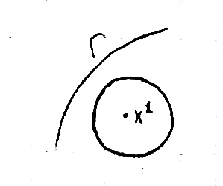
\includegraphics[scale = 0.7]{29_1_new}
\end{center}

Возьмем шар $B(x^1, \cfrac{\delta_1}{2}) = \{ x \in \R^3 : |x - x^1| < \cfrac{\delta_1}{2}\}$. Тогда расстояние от произвольной точки $x \in \overline{B(x^1, \cfrac{\delta_1}{2})} \text{ до } \forall y \in \text{Г} \text{ не меньше } \cfrac{\delta_1}{2} : |x-y| \geqslant |x^1-y|-|x-x^1| \geqslant \delta_1 - \cfrac{\delta_1}{2} = \cfrac{\delta_1}{2} $

Поэтому $\cfrac{1}{|x-y|} \in C^\infty(\underbrace{\overline{B(x^1, \cfrac{\delta_1}{2})}}_x \times \underbrace{\text{Г}}_y)\Rightarrow \mathcal{D}_x^\alpha\cfrac{1}{|x-y|} \in C(\overline{B(x^1, \cfrac{\delta_1}{2})} \times \text{Г})$

По теореме о дифференцировании интеграла по параметру (формулировка в билете 5) имеем
\[
\mathcal{D}_x^\alpha V^{(0)}(x) = \int_{\text{Г}} \mathcal{D}_x^\alpha\cfrac{\mu(y)}{|x-y|} dS_y \in C(\overline{B(x^1, \cfrac{\delta_1}{2})} \times \text{Г})\Forall\alpha\text{-мультииндекса}
\]
В частности, $\bigtriangleup_x V^{(0)}(x) = \int_{\text{Г}} \bigtriangleup_x(\cfrac{1}{|x-y|})\mu(y) dS_y = 0$, что и требовалось.
\item[1.] Если $x \in \text{Г, то } \cfrac{1}{|x-y|}$ - полярное ядро, следовательно, интегральный оператор с полярным ядром переводит непрерывную функцию $\mu(y)$ в непрерывную $\Rightarrow V^{(0)}(x) \in C(\text{Г})$.

Мы уже доказали, что $V^{(0)}(x) \in C(\R^3 \backslash \text{Г}) \Rightarrow$ осталось показать непрерывность в областях $\Omega$ следующего вида:

\begin{center}
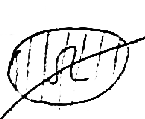
\includegraphics[scale = 0.6]{29_2_new}
\end{center}



Построим для этого последовательность функций, равномерно сходящихся к $V^{(0)}(x)$:

Пусть $\biggl(\cfrac{1}{|x-y|}\biggr)_\delta - \delta\text{-срезка функции } \cfrac{1}{|x-y|}: $
\[
\biggl(\cfrac{1}{|x-y|}\biggr)_\delta=\begin{cases}
\cfrac{1}{|x-y|},&\text{если $|x-y|\geqslant \delta$;}\\
\cfrac{1}{\delta},&\text{если $|x-y|<\delta$.}
\end{cases}
\]
$V^{(0)}_\delta(x) = \int_{\text{Г}} \biggl(\cfrac{1}{|x-y|}\biggr)_\delta\mu(y) dS_y \in C(\overline{\Omega})$

Будем выбирать $0 < \delta < \cfrac{d}{2} (d - \text{из свойств области с границей класса }C^2) - \text{ такое число, что }\forall x^0 \in \text{Г} \rightarrow B(x^0, d) \subset U_{x^0}$
\[
\biggl| V^{(0)}(x) - V_\delta^{(0)}(x) \biggr| = \biggl| \int_{\text{Г}} \Biggl(\cfrac{1}{|x-y|} - \biggl(\cfrac{1}{|x-y|}\biggr)_\delta\Biggr)\mu(y) dS_y \biggr|
\]

Если $x : |x-y| \geqslant \delta$, то $ \Biggl(\cfrac{1}{|x-y|} - \biggl(\cfrac{1}{|x-y|}\biggr)_\delta\Biggr)= 0 $

В противном случае она равна $\biggl|\int_\text{Г}\underbrace{(\cfrac{1}{|x-y|} - \cfrac{1}{\delta})}_{>0}\underbrace{\mu(y)}_{|\mu(y)| \leqslant  ||\mu||_{C(\text{Г})} = C} dS_y \biggr| \geqslant C\int\limits_{\substack{y \in \text{Г} \\ |x-y|<\delta}}\cfrac{dS_y}{|x-y|}$


Нам осталось оценить интеграл $\int\limits_{\substack{y \in \text{Г} \\ |x-y|<\delta}}\cfrac{dS_y}{|x-y|}$

\begin{center}
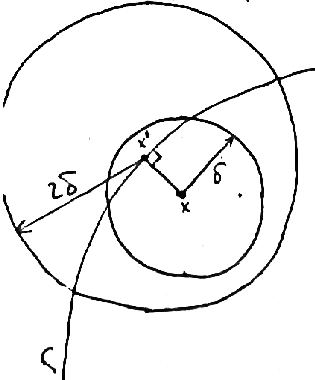
\includegraphics[scale = 0.25]{29_3_new}
\end{center}

Пусть $x^* = \pi_\text{Г}(x)$. Построим $B(x,\delta)$ и $B(x^*, 2\delta)$.

Ясно, что т.к. $|x - x^*| < \delta \Rightarrow B(x, \delta) \subset B(x^*, 2\delta)$.

Увеличивая область интегрирования, запишем:


\[
\int_{\substack{y \in \text{Г} \\ |x-y|<\delta}}\cfrac{dS_y}{|x-y|} \leqslant \int\limits_{\substack{y \in \text{Г} \\ |x^*-y|<2\delta}}\cfrac{dS_y}{|x^*-y|}
\]
По определению числа d имеем $B(x^*, 2\delta \subset U_{x^*})$. 
\begin{center}
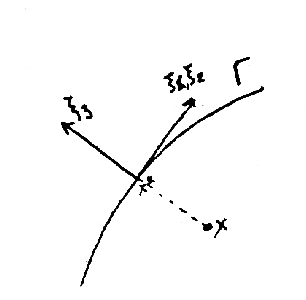
\includegraphics[width=0.2\linewidth]{29_4_new} 
\end{center}

Свяжем с $x^*$ локальную систему координат и функцию $F_{x^*} (\xi_1, \xi_2)$


Т.к. $y \in \text{Г}, y = (\xi_1, \xi_2, F_{x^*}(\xi_1, \xi_2))$

Т.к. $x^* = \pi_\text{Г}(x)$, точка x имеет ненулевую компоненту только по $\xi_3\ :\ x = (0,0,x_3)$


Оценки: $|x-y|^2 = \xi_1^2 + \xi_2^2 + (x_3 - F_{x^*}(\xi_1, \xi_2))^2 \leqslant \xi_1^2 + \xi_2^2$ \\ 
$|x^*-y|^2 = \xi_1^2 + \xi_2^2 + (F_{x^*}(\xi_1, \xi_2))^2 \leqslant \xi_1^2 + \xi_2^2 \Rightarrow$ расширяем область интегрирования до $\sqrt{\xi_1^2 + \xi_2^2} < 2\delta$
\[
\biggl| V^{(0)}(x) - V_\delta^{(0)}(x) \biggr| \geqslant C \int\limits_{\sqrt{\xi_1^2 + \xi_2^2} < 2\delta} \cfrac{\sqrt{1 + (\pd{F_{x^*}}{\xi_1}(\xi_1, \xi_2))^2 +  (\pd{F_{x^*}}{\xi_2}(\xi_1, \xi_2))^2}}{\sqrt{\xi_1^2 + \xi_2^2}}d\xi_1d\xi_2 \leq
\] 
\[C \sqrt{1 + 2M_1^2} \int\limits_{\sqrt{\xi_1^2 + \xi_2^2} < 2\delta} \cfrac{d\xi_1d\xi_2}{\sqrt{\xi_1^2 + \xi_2^2}}
\]

В полярной системе координат $\bigl(\begin{smallmatrix}
\xi_1 \\ \xi_2
\end{smallmatrix}\bigr) = r \bigl(\begin{smallmatrix}
\cos \varphi \\ \sin \varphi
\end{smallmatrix}\bigr)$ последний интеграл примет вид $\int\limits_{0}^{2\pi}d\varphi \int\limits_{0}^{2\delta}\cfrac{rdr}{r} = 4\pi\delta \rightarrow 0 \text{ при } \delta \rightarrow 0.$

Итак, $\underbrace{V_\delta^{(0)}(x)}_{\in C(\overline{\Omega})}\rightrightarrows_{\delta \rightarrow 0} V^{(0)}(x) \Rightarrow V^{(0)}(x) \in C(\overline{\Omega})\Rightarrow V^{(0)}(x) \in C(\R^3)$.

\item[3.] $\mu(x) \in \text{Г}\Rightarrow |\mu(x)|\leqslant ||\mu||_{\text{Г}} = C \Forall x \in \text{Г}$

Возьмем сферу радиуса R такую, что Г лежит внутри этой сферы. Тогда $\forall y \in \text{Г} \rightarrow |y| \leqslant R.$

При $x \rightarrow \infty\  \rightarrow |x|\geqslant 2R\ \Rightarrow y \leqslant \cfrac{|x|}{2} \ \Rightarrow |V^0(x)| \leqslant \int_{\text{Г}}\cfrac{|\mu(y)|}{|x-y|}dS_y \leqslant \cfrac{2C}{|x|}\underbrace{\int_\text{Г}dS_y}_{\mathbf{\vec C}} \Rightarrow V^0(x) = O(\cfrac{1}{|x|}) \text{ при } x \rightarrow \infty.$
\end{enumerate}
\end{proof}
\newpage
\section{Потенциал двойного слоя. Интеграл Гаусса. Скачок потенциала двойного слоя при переходе через границу, на которой задаётся плотность}
% Затехал: Леонтьев Семён 377 группа

Пусть $\Gamma$ - граница класса $C^2$ ограниченной области $\Omega \subset \R^3$.

\begin{definition}
Функция вида
$V^{(2)}(x) = \int\limits_{\Gamma} \, \frac{\partial}{\partial \bar{n}_y}\brk*{\frac{1}{\abs*{x-y}}}\nu(y) dS_y $
называется \textit{\text{потенциалом двойного слоя}}
\end{definition}

Сразу будет удобно переписать определение в иной форме:
$$ \frac{\partial}{\partial \bar{n}_y}\brk*{\frac{1}{\abs*{x-y}}} = \sum_{k=1}^3 n_k(y)\frac{\partial}{\partial y_k}\frac{1}{\abs*{x-y}} = \sum_{k=1}^3 \frac{n_k(y)(x_k - y_k)}{\abs*{x-y}^3} = \frac{(x-y, \bar{n}_y)}{\abs*{x-y}^3} \Rightarrow $$
$$ \Rightarrow V^{(2)}(x) = \int\limits_{\Gamma} \, \frac{(x-y, \bar{n}_y)}{\abs*{x-y}^3}\nu(y) dS_y $$

\begin{lemma} Пусть $\nu(x) \in C(\Gamma)$. Тогда:

\
а) $V^{(2)}(x)$ - гармоническая функция в в $x\in \R^3\backslash \Gamma$;

\
б) $\displaystyle V^{(2)}(x) = O\brk*{\frac{1}{\abs*{x}^2}}$ при $\abs*{x} \rightarrow \infty$
\end{lemma}

\begin{proof}
\

а) $$ V^{(2)}(x) = \sum_{k=1}^3\int\limits_{\Gamma} 
\
\underbrace{n_k(y)}_{\substack{\in C(\Gamma)\\ \text{т.к.} \Gamma \in C^2}}
\underbrace{\nu(y)}_{\substack{\in C(\Gamma)\\ \text{по}\\ \text{условию}}} 
\
\underbrace{\frac{\partial}{\partial y_k} \frac{1}{\abs*{x-y}}}_{\substack{-\frac{\partial}{\partial x_k} \frac{1}{\abs*{x-y}}\\ \in C\brk*{(\R^3\backslash\Gamma)\times\Gamma}}}dS_y
\
=
\
-\sum_{k=1}^3\frac{\partial}{\partial x_k} \int\limits_{\Gamma}
\
\underbrace{n_x(y)\nu(y)\frac{1}{\abs*{x-y}}dS_y}_{\substack{\text{потенциал простого слоя с}\\  \mu = n_k\cdot\nu\in C(\Gamma)\\ \Downarrow\\ \text{является гармонической}\\ \text{функцией в } R^3\backslash\Gamma}} 
 $$
 Остаётся воспользоваться тем, что производная гармонической функции - гармоническая.
\

б) Возьмём сразу сферу радиуса $R$ такую, что $\Gamma$ лежит внутри сферы. При $$\abs*{x} \rightarrow \infty \Rightarrow \abs*{x}>2R \Rightarrow
\abs*{y} \leq \frac{\abs*{x}}{2} \Rightarrow \abs*{x-y}^2\geq \brk*{\abs*{x} - \abs*{y}}^2 \geq \frac{\abs*{x}}{4}  $$
$$\abs*{\frac{\partial}{\partial\bar{n}_y} \frac{1}{\abs*{x-y}}} \leq \frac{\abs*{x-y}\cdot\abs*{\bar{n}_y}}{\abs*{x-y}^3} = \frac{1}{\abs*{x-y}^2} \Rightarrow$$
$$\Rightarrow\abs*{V^{(2)}(x)} = \abs*{\int\limits_{\Gamma} \, \frac{\partial}{\partial \bar{n}_y}\brk*{\frac{1}{\abs*{x-y}}}\nu(y) dS_y}\leq\frac{4}{\abs*{x}^2}\int\limits_{\Gamma} \, \abs*{\nu(y)}dS_y\leq4\norm*{\nu(y)}_{C(\Gamma)}\int\limits_{\Gamma} dS_y\cdot\frac{1}{\abs*{x}^2 \Rightarrow}$$
$$\Rightarrow V^{(2)}(x) = O\brk*{\frac{1}{\abs*{x}^2}} \text{при} x\rightarrow \infty$$
\end{proof}

\begin{lemma}
Если $\Omega$ ограниченная область с границей $\Gamma \in C^2$, то $\forall x,y\in\Gamma, x\neq y$, справедлива оценка $$\abs*{\frac{(x-y,n(y))}{\abs*{x-y}^2}}\leq\frac{M}{\abs*{x-y}}$$
\end{lemma}
\begin{proof}
Пусть $d$ - число из определения поверхности с границей $\Gamma \in C^2$:
\begin{itemize}[noitemsep]
\item если $\displaystyle  \abs*{x-y}\geq d$, то $\displaystyle \frac{\abs*{(x-y,\bar{n}_y)}}{\abs*{x-y}^3} \leq \frac{1}{\abs*{x-y}^2} \leq \frac{1}{d}\frac{1}{\abs*{x-y}}$
\item если $\abs*{x-y} < d$, то свяжем $y$ с локальной системой координат. В этой системе: 
\

$\displaystyle y=(0,0,0)$, $x = (\xi_1,\xi_2, F(\xi_1, \xi_2))$, $\bar{n}_y = (0,0,1) \Rightarrow$
\

 $\displaystyle \abs*{x-y, \bar{n}_y)} = \abs*{F_y(\xi_1, \xi_2)} \leq M_2(\xi_1^2+\xi_2^2)\leq M_2(\xi_1^2+\xi_2^2 + F_y^2(\xi_1, \xi_2) = M_2\abs*{x-y}^2$, что и требовалось.
\end{itemize}
\end{proof}
\begin{lemma}
Пусть $\nu(x) \in C(\Gamma)$. Тогда потенциал двойного слоя $V^{(2)} \in C(\Gamma)$
\end{lemma}

\begin{proof}
Используем признак полярного ядра (билет №24). В силу леммы $\abs*{K(x,y)} \leq \frac{M}{\abs*{x-y}}$ и 
\
$K(x,y) = \displaystyle \frac{(x-y, \bar{n}_y)}{\abs*{x-y}^2}\in C\brk*{(\Gamma\times\Gamma)\backslash \brk[c]*{x=y}}$
Оператор с полярным ядром переводит непрерывные функции в непрерывные, а $\nu \in C(\Gamma) \Rightarrow V^{(2)}(x)\in C(\Gamma)$

\end{proof}
Наша цель - описать скачок $V^{(2)}(x)$ при переходе через границу. Для этого потребуется несколько вспомогательных утверждений.
\begin{lemma}
Пусть $\Omega$ - ограниченная область с границей $\Gamma\in C^2$. Тогда интеграл $\displaystyle V^{(2)}_{GAUSS}(x) = 
\int\limits_{\Gamma} \frac{\partial}{\partial\bar{n}_y}\brk*{\frac{1}{\abs*{x-y}}}\nu(y) \cdot 1 \cdot dS_y = \dfrac{(x-y, \bar{n}_y)}{\abs*{x-y}^3} dS_y$ - (интеграл Гаусса) равен 

$\begin{cases} -4\pi, x\in \Omega \\
-2\pi, x\in \Gamma \\ 0, x\in\R^3\backslash \overline{\Omega}
\end{cases}$
\end{lemma}

\begin{proof}
1) Пусть $x \in \Omega$. Возьмём $u(x)\equiv 1$ и запишем представление этой функции в виде суммы трёх потенциалов:
$$u(x) \equiv 1 = \int\limits_{\Omega} \brk*{\frac{-1}{4\pi\abs*{x-y}}}\underbrace{\Delta 1}_{\substack{ = 0}} dy + \int\limits_{\Gamma}\frac{\partial}{\partial \bar{n}_y}\brk*{\frac{-1}{4\pi\abs*{x-y}}}u(y)dS_y - \int\limits_{\Gamma}\brk*{\frac{-1}{4\pi\abs*{x-y}}}
\
\underbrace{\frac{\partial u(y)}{\bar{n}_y}}_{\substack{ = 0}}
\
=
\
-\frac{1}{4\pi}V_{GAUSS}^{(2)}(x)
$$
2) Пусть $x \in \R^3\backslash \overline{\Omega}$ 
Возьмём $u(y) \equiv 1$ и $v(y) = \frac{1}{\abs*{x-y}}$ и воспользуемся для этих функций первой формулой Грина:
$$\int\limits_{\Omega} \underbrace{\Delta_y v(y)}_{\substack{ = 0}} \cdot u(y)dy = \underbrace{\int\limits_{\Gamma}\frac{\partial}{\partial \bar{n}_y}v(y)u(y)dS_y}_{\substack{ = V_{GAUSS}^{(2)}(x)}}
-
\underbrace{\int\limits_{\Omega}\brk*{\nabla_y v(y), \nabla 1}dy}_{\substack{ = 0}}
\Rightarrow
V_{GAUSS}^{(2)}(x) = 0
$$
3) Пусть $x\in \Gamma$. Введём $B = B(x,\varepsilon), \Omega_\varepsilon = \Omega\backslash\bar{B}, \Gamma_\varepsilon = \Gamma\backslash B, \sigma_\varepsilon = \partial B\cap \bar{\Omega} $
Тогда $\partial \Omega_\varepsilon = \Gamma_\varepsilon \cup\sigma_\varepsilon \Rightarrow x\in \R^3 \backslash \bar{\Omega}_\varepsilon$
\begin{center}
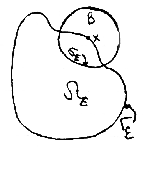
\includegraphics[width=0.2\textwidth]{30_1_new}
\end{center}
Согласно второму пункту можем написать $\displaystyle\int\limits_{\partial \Omega_\varepsilon}\dfrac{\partial}{\partial \bar{n}_y}\brk*{\dfrac{1}{\abs*{x-y}}} dS_y = 0$
Значит $$\underbrace{\int\limits_{\Gamma_\varepsilon} \frac{\partial}{\partial \bar{n}_y}\brk*{\frac{1}{\abs*{x-y}}} dS_y}_{\substack{\rightarrow \int\limits_{\Gamma} \text{при } \varepsilon \rightarrow 0}}
+
 \int\limits_{\sigma_\varepsilon} \frac{\partial}{\partial \bar{n}_y}\brk*{\frac{1}{\abs*{x-y}}} dS_y = 0 $$
 Покажем, что $$\displaystyle\int\limits_{\sigma_\varepsilon} \dfrac{\partial}{\partial \bar{n}_y}\brk*{\dfrac{1}{\abs*{x-y}}} dS_y \rightarrow 2\pi \text{ при } \varepsilon \rightarrow 0 \text{ } \dfrac{\partial}{\partial \bar{n}_y}\brk*{\dfrac{1}{\abs*{x-y}}} = \dfrac{(x-y, \bar{n}_y)}{\abs*{x-y}^3} = \dfrac{\abs*{x-y}\abs*{\bar{n}_y}}{\abs*{x-y}^3} 
=
\dfrac{1}{\abs*{x-y}^2} = \dfrac{1}{\eps^2} $$
Поэтому $\displaystyle\int\limits_{\sigma_\varepsilon} \dfrac{\partial}{\partial \bar{n}_y}\brk*{\dfrac{1}{\abs*{x-y}}} dS_y = \dfrac{1}{\varepsilon^2}\int\limits_{\sigma_\varepsilon}dS_y$
\

При малых $\varepsilon$ кусок границы $\Gamma$ внутри $\rightarrow$ к полуплоскости $\Rightarrow \sigma_\varepsilon \rightarrow$ к полусфере.
\

Поэтому  $\int\limits_{\sigma_\varepsilon}dS_y = 2\pi\varepsilon^2\brk*{1+O(1)}$, что и требовалось
\end{proof}

$\bf{Offtop:}$ Геометрический смысл интеграла Гаусса: 
$\dfrac{(y-x, \bar{n}_y)}{\abs*{x-y}^3}dS_y = \dfrac{dS_ycos\beta}{\abs*{x-y}^2} = d\Omega$
\begin{center}
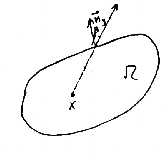
\includegraphics[width=0.2\textwidth]{30_2_new}
\end{center}

-- телесный угол, под которым из точки $x$ видна часть $dS_y$. Интеграл Гаусса есть сумма всех таких углов со знаком $"\text{минус}"$. Поэтому геометрически последняя лемма очевидна.


\begin{lemma}
Пусть $\Omega$ - ограниченная область в $\R^3$  с границей $\Gamma \in C^2$. Пусть $x^o \in \Gamma$. Тогда
\

 $\forall x: (x\in \R^3)\cap\brk*{\abs*{x-x^o}<\dfrac{d_*}{2}} $ верно $\displaystyle\int\limits_{\abs*{y-x^o}<d_*}\dfrac{(x-y, \bar{n}_y)}{\abs*{x-y}^3}dS_y <K, d_* = \dfrac{1}{2}min\brk*{d, \dfrac{2}{M_2}}
$
\

Без доказательства
\end{lemma}
\begin{lemma}
Пусть $\Omega$ - ограниченная область в $\R^3$ с границей $\Gamma \in C^2$. Пусть $x^o\in \Gamma$. Тогда 
$\displaystyle\lim_{x \to x^o} W(x, x^o) = W(x^o, x^o)$, где $W(x, x^o) = \displaystyle\int\limits_{\abs*{y-x^o}<d_*}\dfrac{(x-y, \bar{n}_y)}{\abs*{x-y}^3}\brk*{\nu(y) - \nu(x^o)}dS_y$,  а $\nu(x)\in C(\Gamma)$
\end{lemma}

\begin{proof}
Требуется показать, что $ \forall \varepsilon>0 \Exists \delta_\varepsilon>0: \Forall x: \abs*{x-x^o} < \delta_\varepsilon \rightarrow \abs*{W(x,x^o) - W(x^o, x^o)} < \varepsilon.
$
Функция $\nu(x)$ непрерывна на компакте, следовательно она и равномерно непрерывна на нём. Значит 
$\exists \beta = \beta(\varepsilon): \Forall y \in \Gamma: \abs*{y-x^o}<\delta \rightarrow \abs*{\nu(y) - \nu(x^o)} <\varepsilon
$
. Выберем $\beta \leq \dfrac{d_*}{2}$
$$
\abs*{W(x,x^o) - W(x^o,x^o)} = \abs*{\displaystyle\int\limits_{\Gamma}\brk*{\dfrac{(x-y, \bar{n}_y)}{\abs*{x-y}^3} 
-
\dfrac{(x^o-y, \bar{n}_y)}{\abs*{x^o-y}^3} }\brk*{\nu(y) - \nu(x^o)}dS_y} 
\leq
$$
$$
\leq
\displaystyle\int\limits_{\abs*{y-x^o}<\beta}\underbrace{\brk*{\dfrac{(x-y, \bar{n}_y)}{\abs*{x-y}^3} 
-
\dfrac{(x^o-y, \bar{n}_y)}{\abs*{x^o-y}^3} }}_{\substack{\leq K+K}}
\underbrace{\brk*{\nu(y) - \nu(x^o)}}_{\substack{\leq \varepsilon}}dS_y 
\
+$$ $$
\
\displaystyle\int\limits_{\Gamma\backslash\brk*{\abs*{y-x^o}<\beta}}\underbrace{\brk*{\dfrac{(x-y, \bar{n}_y)}{\abs*{x-y}^3} 
-
\dfrac{(x^o-y, \bar{n}_y)}{\abs*{x^o-y}^3} }}_{\substack{\leq \psi(x); \psi(x^o) = 0 \\ 
\Downarrow \\
\exists \delta_1: \norm*{\psi(x)}< \varepsilon,\\
\text{если} \abs*{x-x^o} < \delta_1 
}}
\underbrace{\brk*{\nu(y) - \nu(x^o)}}_{\substack{\leq 2\norm*{\nu}_{C(\Gamma)}}}dS_y 
$$

Значит, при $\abs*{x-x^o}\leq max \brk*{\dfrac{d_*}{2}, \delta_1(\varepsilon)}$
имеет место оценка 
$\abs*{W(x, x^o) - W(x^o, x^o)} \leq 2K\varepsilon + 2\varepsilon\norm*{\nu}_{C(\Gamma)}
$
\end{proof}

Теперь можно перейти к описанию скачка потенциала.
\begin{theorem}
Пусть $\Omega$ - ограниченная область в $\R^3$ с границей $\Gamma \in C^2$, а $\nu(x) \in C(\Gamma)$. Тогда потенциал двойного слоя $V^{(2)}(x) \in C(\bar{\Omega})$ и $V^{(2)}(x) \in C(\R^3\backslash\bar{\Omega})$ (можно непрерывно продолжить на замыкания). Обозначим $\forall x^o\in \Gamma: V^{(2)}_+(x^o) = \displaystyle \lim_{x\in \Omega,  x\to x^o} V^{(2)}(x);
V^{(2)}_-(x^o) = \displaystyle \lim_{x\in \R \backslash \bar{\Omega},  x\to x^o} V^{(2)}(x) $ 
Тогда $V^{(2)}_\pm(x^o) = V^{(2)}(x^o) \mp 2\pi\nu(x^o)$
\end{theorem}

\begin{proof}
$$V^{(2)}(x) = W(x, x^o) + \nu(x^o) \int\limits_{\Gamma} \, \frac{(x-y, \bar{n}_y)}{\abs*{x-y}^3}\nu(y) dS_y$$
$$ V^{(2)}_+(x^o) = \displaystyle \lim_{x\in \Omega,  x\to x^o} V^{(2)}(x) =
\underbrace{\displaystyle \lim_{x\in \Omega,  x\to x^o} 
W(x, x^o)}_{\substack{W(x^o,x^o) \\ \text{в силу леммы}}} 
+
 \nu(x^o)\lim_{x\in \Omega,  x\to x^o} \underbrace{\int\limits_{\Gamma} \, \frac{(x-y, \bar{n}_y)}{\abs*{x-y}^3}\nu(y) dS_y}_{\substack{\text{при } x\in \Omega \text{ это }4\pi}}
 = 
 W(x^o, x^o) -4\pi\nu(x^o)
$$
Далее, если $x^o \in \Gamma$, то  $\displaystyle V^{(2)}(x^o) = W(x^o, x^o) + \nu(x^o) \int\limits_{\Gamma} \, \frac{(x^o-y, \bar{n}_y)}{\abs*{x^o-y}^3}\nu(y) dS_y = W(x^o, x^o) -2\pi\nu(x^o)$
\

Поэтому $V^{(2)}_+(x^o) = V^{(2)}_(x^o) -2\pi\nu(x^o)$
Это, в частности, означает, что $V^{(2)}(x)$ можно непрерывно продолжить до $\bar{\Omega}$.
\
Для стремления $x \to x^o$ извне доказательство аналогично:
 $$
 V^{(2)}_-(x^o) = 
\underbrace{\displaystyle \lim_{x\in \R^3 \backslash\Omega,  x\to x^o} 
W(x, x^o)}_{\substack{W(x^o,x^o) \\ \text{в силу леммы}}} 
+
 \lim_{x\in \R^3 \backslash\Omega,\  x\to x^o}\nu(x^o) \underbrace{\int\limits_{\Gamma} \, \frac{(x-y, \bar{n}_y)}{\abs*{x-y}^3}\nu(y) dS_y}_{\substack{\text{при } x\in \R^3 \backslash\Omega \text{ это }0}} = W(x^o, x^o) = V^{(2)}(x^o) + 2\pi\nu(x^o)
$$
Это, в частности, означает, что $V^{(2)}$ можно непрерывно продолжить до $\R^3 \backslash \Omega$ 
\end{proof}

\newpage
\section{ Понятие правильной нормальной производной. Существование правильной нормальной производной у потенциала простого слоя с непрерывной плотностью Формула скачка для нормальной производной}
Мотивация: во внутренней задаче Неймана (билет 14) ищется решение $u(x) \in C^2(\Omega) \cap C^1(\bar{\Omega})$ уравнения $$\Delta u = f(x), x \in \Omega$$ при условии $$\frac{\partial u}{\partial \vec{n}}|_r = u_1(x),$$ где $u_1 \in C(\Gamma)$.

Но существуют примеры гармонических в области функций, градиент которых нельзя продолжить по непрерывности на замыкание этой области. Можно расширить понятие классического решения.

Пусть $u(x) \in C^1(\Omega) \cap C(\bar{\Omega}), \Omega$ - ограниченная область в $\R^3$ с границей $\Gamma \in C^2$
\begin{center}
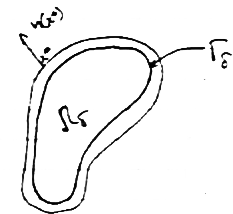
\includegraphics[width=0.2\textwidth]{31_1_new}
\end{center}
Пусть $x^o \in \Gamma$, а $\vec{n(x^o)}$ - нормаль к $\Gamma$ в $x^o$ Т.к. $\Gamma \in C^2$, $\vec{n(x^o)}$ - непрерывная функция по $x^o$. Проведем через $x^o$ прямую $x = x^o + \vec{n(x^o)}t, t \in \mathbb{R}$

Распишем произведенеие $$(\vec{n}(x^o), \triangledown u) = \sum_{k=1}^{3} n_x(x^o)\frac{\partial u}{\partial x_k}(x) = \frac{du(x^o + \vec{n}(x^o)t)}{dt} = \frac{\partial u}{\partial \vec{n}(x^o)}$$

\begin{definition}
Говорят, что $u(x)$ имеет \textbf{правильную нормальную производную} по направлению внешней нормали на $\Gamma$ из $\Omega$, если  
\begin{enumerate}
\item $\forall x^o \in \Gamma$ существует конечный предел 
$$\frac{\partial u}{\partial \vec{n}}(x^o) \equiv \lim_{x = x^o + \vec{n}(x^o)t,\\ x \in \Omega, \\ x \to x^o} \frac{\partial u}{\partial \vec{n}(x^o)}(x)$$

\item Этот предел равномерный по $x^o \in \Gamma$
\end{enumerate}
\end{definition}
\begin{lemma}
Если u(x) имеет ПНП по нормали $\vec{n}(x^o)$ из $\Omega$ на $\Gamma$, то 
\begin{enumerate}
\item u(x) имеет обычную производную по нормали $\vec{n}(x^o)$ в точке $x^o \in \Gamma$, и эта производная совпадает с ПНП 

\item ПНП $\in C(\Gamma)$
\end{enumerate}
\end{lemma}
\begin{proof} Обычная производная по нормали $$\lim_{x \to x^o, x = x^o + \vec{n}(x^o)t} \frac{u(x^o) - u(x)}{|x^o - x|} = \lim_{t < 0, t \to 0} \frac{u(x^o - u(x^o + \vec{n}(x^o)t))}{-t} = \lim_{t < 0. t \to 0} \frac{du(x^o + \vec{n}(x^o)t)}{dt} = \frac{\partial u}{\partial \vec{n}(x^o)}$$ - этот предел существует по условию.

Покажем непрерывность: Пусть $\delta$ мало, $0 < \delta < \delta_o, x = x^o - \delta n(x^o)$

Пусть $V_{\delta}(x^o) = \frac{\partial u}{\partial \vec{n}}(x^o - \delta \vec{n}(x^o))= $

$$=\sum_{k=1}^{3} n_k(x^o)\frac{\partial u}{\partial x_n}(x^o - \delta \vec{n}(x^o)) => V_{\delta}(x^*) \in C(\Gamma) $$

$n_k(x^o)$ непрерывна, т.к. $\Gamma \in C^2$

По определению ПНП: $V_{\delta} \rightrightarrows $ ПНП => она также непрерывная на $\Gamma$. 
\end{proof}
$\bullet$ После расширения определения классического решения встает вопрос о единственности решения. При исследовании этого вопроса мы использовали формулы Грина. Дли них требовалось гладкость $C^2(\Omega) \cap C^1(\bar{\Omega})$. Покажем, как обобщить эти факты с помощью ПНП.

$\bullet$ Пусть $\Omega$ - ограниченная область с границей $\R^3$, граница $G \in C^2, 0 < \delta < \delta_{\mu}$

$\Gamma_{\delta} = {x: x = x^o - \delta \vec{n}(x^o)}$ - граница класса уже $C^1$, т.к. $\vec{n} \ in C^1$
\begin{center}
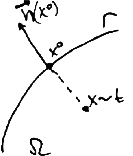
\includegraphics[width=0.2\textwidth]{31_2_new}
\end{center}
\begin{lemma}
Пусть $\Omega$ - ограниченная область с границей $G \in C^2, u(x) \in C^2(\Omega) \cap C(\bar{\Omega})$, а у $u(x) \Exists $ ПНП по направлению внешней нормали $\vec{n}(x^o), \Delta u \in C(\Omega)$. Тогда $$\int_{\Omega} (\Delta u)udx = \oint_{\Gamma} \frac{\partial u}{\partial \vec{n}}(x) u(x)dS - \int_{\Omega} |\triangledown|^2 dx $$
\end{lemma}
\begin{proof}
$u(x) \in C^2(\Omega) \cap C(\bar{\Omega}) => u(x) \in C^2(\Omega_{\delta}) \cap C^1(\Omega_{\delta}) => $

$$\int_{\Omega_{\delta}}(\Delta u(x))u(x)dx (1) = \oint_{G_{\delta}} \frac{\partial u}{\partial \vec{n}}u(x)dS (2) - \int_{\Omega_{\delta}}|\triangledown u(x)|^2dx (3)$$

$\lim_{\delta \to 0}(1) = \int_{\Omega} \Delta udx$, т.к. $\Delta u(x)$ и $u(x) \in C(\bar{\Omega})$

$\lim_{\delta \to 0}(2) = \int_{G_{\delta}} \frac{\partial u}{\partial \vec{n}}u(x)dS $

$\lim_{\delta \to 0}(3) = \lim_{x = x^o - \delta \vec{n}x^o} \int_{\Omega_{\delta}} |\triangledown u(x)|^2dx$

$\bullet$ С учетом сделанного обобщения все сделанные ранее рассуждения о внутренних и внешних задачах верны и для расширенного понятия классического решения.
\end{proof}
\begin{theorem}[Кореектная постановка внутренней задачи Неймана для уравнения Лапласа]
$\Omega$ - ограниченная область, граница $G \in C^2$. Найти функцию $u(x) \in C^2(\Omega) \cap C(\bar{\Omega})$, имеющую ПНП и удовлетворяющую 

\begin{equation}
\begin{cases}
\Delta u(x) = 0, x \in \Omega
\\
\frac{\partial u}{\partial \vec{n}}|_G = u_1(x) \in C(G)
\end{cases}
\end{equation}
\end{theorem}
\begin{theorem}[Корректная постановка внешней задачи Неймана для уравнения Лапласа]
$\Omega$ - внешняя область, граница $G \in C^2$. Найти функцию $u(x) \in C^2(\Omega) \cap C(\bar{\Omega})$ имеющую ПНП и удовлетворяющую 
\begin{equation}
\begin{cases}
\Delta u(x) = 0, x \in \Omega
\\
\frac{\partial u}{\partial \vec{n}}|_{\Gamma} = u_1(x) \in C(\Gamma)
\\
u(x)_{x \to \infty} \to 0
\end{cases}
\end{equation}
\end{theorem}
$\bullet$ Рассмотрим потенциал простого слоя

$\Omega$ - ограниченная область с границей $\Gamma \in C^2; x = x^o - \delta \vec{n}(x^o); 0 < \delta < \delta^*$
  $$V^* = \int_{\Gamma} \frac{\mu(x)}{|x - y|}dS_y$$

$$\frac{\partial u}{\partial \vec{n}}(x) = \sum_{k = 1}^3 n_k(x^o) \frac{\partial}{\partial x_k}\oint_{\Gamma} \frac{\mu(x)}{|x - y|}dS_y = \sum_{k = 1}^3 n_k(x^o) \frac{\partial}{\partial x_k}\oint_G \frac{1}{|x - y|}\mu(y)dS_y$$

$$\sum_{k = 1}^3 n_k(x^o) \frac{\partial}{\partial x_k} \frac{1}{|x - y|}\mu(y)dS_y = \oint_{\Gamma} \sum_{k = 1}^3 n_k(x^o) \frac{y_k - x_k}{|x - y|^3}\mu(y)dS_y = \oint_{\Gamma} \frac{(y - x, \vec{n}(x^o))}{|x - y|^3}\mu(y)dS_y$$

Обозначим $\left( \frac{\partial V^o}{\partial \vec{n}} \right)_{\pm}(x^o) = \lim_{x = x^o \mp \delta \vec{n}(x)}, \delta \to +0 \frac{\partial V^o}{\partial \vec{n}(x^o)} (x)$

$\frac{\partial V^o)}{\partial \vec{n}}(x^o)(1) = \int_{\Gamma} \frac{(y - x^o, \vec{n}(x^o))}{|x^o - y|^3}\mu(y)dS_y, x^o \in G(2)$

(1) - прямое значение нормальной производной

(2) - полярное ядро => $\forall \mu(x) \in C(G), \Forall x^o \in \Gamma$ этот интеграл существует, и более того $(1) \in C(\Gamma)$

\begin{theorem}
У потенциала простого слоя $V^o(x)$ с плотностью $\mu(x) \in C(\Gamma)$ существует ПНП на $\Gamma$: $$\left( \frac{\partial V^o}{\partial \vec{n}}_+(x^o)\right)
\text{и} \left(\frac{\partial V^o}{\partial \vec{n}}_-(x^o) \right),$$
причем имеет место формула скачка 

$$\left(\frac{\partial V^o}{\partial \vec{n}}_{\pm}(x^o) \right) = \frac{\partial V^o}{\partial \vec{n}}(x^o) \pm 2\pi \mu(x^o) $$
\end{theorem}
\begin{conseq}
$\left(\frac{\partial V^o}{\partial \vec{n}} \right)_+(x^o) - \left(\frac{\partial V^o}{\partial \vec{n}} \right)_-(x^o) = 4\pi \mu(x^o), x^o \in \Gamma$

$\frac{\partial V^o}{\partial \vec{n}}(x^o) = \frac{1}{2} \left[ \left(\frac{\partial V^o}{\partial \vec{n}} \right)_+(x^o) + \left(\frac{\partial V^o}{\partial \vec{n}} \right)_=(x^o)\right], x \in \Gamma$
\end{conseq}

\newpage
\section{Билет 32. Сведение с помощью потенциалов внутренней задачи Дирихле и внешней задачи Неймана для уравнения Лапласа к интегральным уравнениям на границе. Существование и единственность решения этих задач}

\subsection{Внешняя задача Неймана для уравнения Лапласа}

Найти функцию $u(x) \in C^2(\R^3 \ \Omega) \cap C(\R^3 \ \Omega)$ имеющую ПНП по направлению внешней нормали, и такую, что 

\begin{equation}
 \begin{cases}
 \Delta u(x) = 0, x \in R^3 \ \Omega
  \\
   (\frac{\partial u}{\partial \vec{n}})_{-}|_r = u_1(x), x \in G; u_1(x) \in C(G)
   \\
   u(x) \to 0, x \to \infty
 \end{cases}
\end{equation}
Решение этой задачи ищем в виде потенциала простого слоя: 

$u(x) = \int_G \frac{\mu(x)}{|x - y|} dS_y$. Свойства $\Delta u(x) = 0$ и $\lim_{x \to \infty} u(x) \to 0$ выполнены.

Кроме того, $u(x) \in C^2(\R^3 | \Omega) \cap C(R^3 | \Omega)$ и имеет ПНП. Нужно проверить $(\frac{\partial u}{\partial \vec{n}})_-|_r = u_1(x), x \in G$. 

$\bullet$ Пусть $$x^o \in G \Rightarrow (\frac{\partial u}{\partial \vec{n}})_{-}(x^o) = -2\pi \mu(x^o) + \int_x \frac{(y - x, \vec{n}(x^o))}{|x^o - y|^3}\mu(y)dS_y = u_1(x^o)$$

$\mu(x^o) = \frac{1}{2\pi}\int_x \frac{(y - x, \vec{n}(x^o))}{|x^o - y|^2}\mu(y)dS_y - \frac{1}{2\pi}u_1(x^o), x^o \in G $ - Интегральное уравнение Фредгольма 2-го рода с интегральным оператором и полярным ядром.

Уравнение однозначно разрешимо $\Leftrightarrow$ уравнение $\mu_*(x^o) = \frac{1}{2\pi}\int_x \frac{(y - x, \vec{n}(x^o))}{|x^o - y|^3}\mu(y)dS_y \equiv 0 $ имеет только тривиальное решение. 

Для этого покажем, что $V_*(x) = \int_G \frac{\mu(x)}{|x - y|}dS_y \equiv 0$

Ясно, что уравнение на $\mu_*$ получается таким же образом как и уравнение на $\mu$, но из задачи Неймана 
\begin{equation}
 \begin{cases}
 \Delta v(x) = 0, x \in R^3 | \Omega
  \\
   (\frac{\partial u}{\partial \vec{n}})|_r = 0, x \in G; u_1(x) \in C(G)
   \\
   u(x) \to 0
 \end{cases}
\end{equation}
В силу единственности решение этой задачи $V_* = 0 (x \in \R^3 | \Omega)$ . Но $V_* \in C(\R^3) \Rightarrow X_* \equiv 0$ на $X \in \R^3 | \Omega$ Функция $V_*$ удовлетворяет внутренней задаче Дирихле

\begin{equation}
 \begin{cases}
 \Delta V_* = 0 \forall x \in \Omega
  \\
  V_*(x) = 0 \forall x \in G
 \end{cases}
\end{equation}

$\Rightarrow V_* \equiv 0 \forall x \in \Omega$

Итак, $V_*(x) \equiv 0 \forall \in R^3$. 

Но $(\frac{\partial u}{\partial \vec{n}})|_+(x^o) - (\frac{\partial u}{\partial \vec{n}})|_-(x^o) = 4\pi \mu_*(x^o), x^o \in G \Rightarrow \mu_*(x^o) \equiv 0 \forall x^o \in G$

Итак, по теореме Фредгольма об альтернативе уравнение 

(*) $\mu(x^o) = \frac{1}{2\pi}\int_x \frac{(y - x, \vec{n}(x^o))}{|x^o - y|^3}\mu(y)dS_y - \frac{1}{2\pi}u_1(x^o), x \in G$ однозначно разрешимо

\subsection{Внутренняя задача Дирихле для уравнения Лапласа}

Найти функцию $u(x) \in C^2(\Omega) \cap C(\bar{\Omega})$ такую, что:

1)$\Delta u(x) = 0, x \in \Omega$

2)$u|_r = u_0(x), x \in G (u_o(x) \in C(G))$ 

Решение этой задачи ищем в виде потенциала двойного слоя 

$u(x) = \frac{1}{2\pi}\int_x \frac{(y - x, \vec{n}(x^o))}{|x^o - y|^3}\nu(y)dS_y, \nu(x) \in C(G)$

Условия $\Delta u = 0 \in \Omega$ и $u(x) \in C^2(G) \cap C(\bar{\Omega})$ уже выполнены. Осталось проверить $u|_r = u_0(x), x \in G$

$\bullet$ Для потенциала двойного слоя справедлива формула скачка: $u_+(x^o) = u(x^o) - 2\pi\nu(x^o) \Rightarrow u_0(x^o) = \int_x \frac{(y - x, \vec{n}(x^o))}{|x^o - y|^3}\nu(y)dS_y - 2\pi\nu(x^o)$

$\Rightarrow \nu(x^o) = \int_x \frac{(y - x, \vec{n}(x^o))}{|x^o - y|^3}\nu(y)dS_y - \frac{u_0(x^o)}{2\pi}, x^o \in G$ Ядро, транспонированное к тому, что стоит в (*) 

Т.к. (*) однозначно разрешмимо, это уравнение тоже имеет единственное решение

\begin{theorem} Пусть $\Omega$ - ограниченная область в $\R^3$ с границей $G \in C^2$. Тогда у внутренней задачи Дирихле $\forall u_1 \in C(G)$, а также у внешней задачи Неймана $\forall u_0 \in C(G)$ существует единственное классическое решение
\end{theorem} 




\end{document}
